% UCL Thesis LaTeX Template
%  (c) Ian Kirker, 2014
% 
% This is a template/skeleton for PhD/MPhil/MRes theses.
%
% It uses a rather split-up file structure because this tends to
%  work well for large, complex documents.
% We suggest using one file per chapter, but you may wish to use more
%  or fewer separate files than that.
% We've also separated out various bits of configuration into their
%  own files, to keep everything neat.
% Note that the \input command just streams in whatever file you give
%  it, while the \include command adds a page break, and does some
%  extra organisation to make compilation faster. Note that you can't
%  use \include inside an \include-d file.
% We suggest using \input for settings and configuration files that
%  you always want to use, and \include for each section of content.
% If you do that, it also means you can use the \includeonly statement
%  to only compile up the section you're currently interested in.
% You might also want to put figures into their own files to be \input.

% For more information on \input and \include, see:
%  http://tex.stackexchange.com/questions/246/when-should-i-use-input-vs-include


% Formatting rules for theses are here: 
%  http://www.ucl.ac.uk/current-students/research_degrees/thesis_formatting
% Binding and submitting guidelines are here:
%  http://www.ucl.ac.uk/current-students/research_degrees/thesis_binding_submission

% This package goes first and foremost, because it checks all 
%  your syntax for mistakes and some old-fashioned LaTeX commands.
% Note that normally you should load your documentclass before 
%  packages, because some packages change behaviour based on
%  your document settings.
% Also, for those confused by the RequirePackage here vs usepackage
%  elsewhere, usepackage cannot be used before the documentclass
%  command, while RequirePackage can. That's the only functional
%  difference as far as I'm aware.
\RequirePackage[l2tabu, orthodox]{nag}


% ------ Main document class specification ------
% The draft option here prevents images being inserted,
%  and adds chunky black bars to boxes that are exceeding 
%  the page width (to show that they are).
% The oneside option can optionally be replaced by twoside if
%  you intend to print double-sided. Note that this is
%  *specifically permitted* by the UCL thesis formatting
%  guidelines.
%
% Valid options in terms of type are:
%  phd
%  mres
%  mphil
%\documentclass[12pt,phd,draft,a4paper,oneside]{ucl_thesis}
\documentclass[12pt,phd,a4paper,oneside]{ucl_thesis}


% Package configuration:
%  LaTeX uses "packages" to add extra commands and features.
%  There are quite a few useful ones, so we've put them in a 
%   separate file.
% -------- Packages --------

% This package just gives you a quick way to dump in some sample text.
% You can remove it -- it's just here for the examples.
\usepackage{blindtext}

% This package means empty pages (pages with no text) won't get stuff
%  like chapter names at the top of the page. It's mostly cosmetic.
\usepackage{emptypage}

% The graphicx package adds the \includegraphics command,
%  which is your basic command for adding a picture.
\usepackage{graphicx}
% Use this command to keep your images in a separate
%  'images' folder.
\graphicspath{ {images/} }

% The float package improves LaTeX's handling of floats,
%  and also adds the option to *force* LaTeX to put the float
%  HERE, with the [H] option to the float environment.
\usepackage{float}

% The amsmath package enhances the various ways of including
%  maths, including adding the align environment for aligned
%  equations.
\usepackage{amsmath}
\usepackage{amsfonts}

% Use these two packages together -- they define symbols
%  for e.g. units that you can use in both text and math mode.
\usepackage{gensymb}
\usepackage{textcomp}
% You may also want the units package for making little
%  fractions for unit specifications.
%\usepackage{units}


% The setspace package lets you use 1.5-sized or double line spacing.
\usepackage{setspace}
\setstretch{1.5}

% That just does body text -- if you want to expand *everything*,
%  including footnotes and tables, use this instead:
%\renewcommand{\baselinestretch}{1.5}


% PGFPlots is either a really clunky or really good way to add graphs
%  into your document, depending on your point of view.
% There's waaaaay too much information on using this to cover here,
%  so, you might want to start here:
%   http://pgfplots.sourceforge.net/
%  or here:
%   http://pgfplots.sourceforge.net/pgfplots.pdf
%\usepackage{pgfplots}
%\pgfplotsset{compat=1.3} % <- this fixed axis labels in the version I was using

% PGFPlotsTable can help you make tables a little more easily than
%  usual in LaTeX.
% If you're going to have to paste data in a lot, I'd suggest using it.
%  You might want to start with the manual, here:
%  http://pgfplots.sourceforge.net/pgfplotstable.pdf
%\usepackage{pgfplotstable}

% These settings are also recommended for using with pgfplotstable.
%\pgfplotstableset{
%	% these columns/<colname>/.style={<options>} things define a style
%	% which applies to <colname> only.
%	empty cells with={--}, % replace empty cells with '--'
%	every head row/.style={before row=\toprule,after row=\midrule},
%	every last row/.style={after row=\bottomrule}
%}

\usepackage{pdflscape}
\usepackage{afterpage}
\usepackage{capt-of}

% The mhchem package provides chemistry formula typesetting commands
%  e.g. \ce{H2O}
%\usepackage[version=3]{mhchem}

% And the chemfig package gives a weird command for adding Lewis 
%  diagrams, for e.g. organic molecules
%\usepackage{chemfig}

% The linenumbers command from the lineno package adds line numbers
%  alongside your text that can be useful for discussing edits 
%  in drafts.
% Remove or comment out the command for proper versions.
%\usepackage[modulo]{lineno}
% \linenumbers 


% Alternatively, you can use the ifdraft package to let you add
%  commands that will only be used in draft versions
%\usepackage{ifdraft}

% For example, the following adds a watermark if the draft mode is on.
%\ifdraft{
%  \usepackage{draftwatermark}
%  \SetWatermarkText{\shortstack{\textsc{Draft Mode}\\ \strut \\ \strut \\ \strut}}
%  \SetWatermarkScale{0.5}
%  \SetWatermarkAngle{90}
%}


% The multirow package adds the option to make cells span 
%  rows in tables.
\usepackage{multirow}


% Subfig allows you to create figures within figures, to, for example,
%  make a single figure with 4 individually labeled and referenceable
%  sub-figures.
% It's quite fiddly to use, so check the documentation.
%\usepackage{subfig}

% The natbib package allows book-type citations commonly used in
%  longer works, and less commonly in science articles (IME).
% e.g. (Saucer et al., 1993) rather than [1]
% More details are here: http://merkel.zoneo.net/Latex/natbib.php
%\usepackage{natbib}

% The bibentry package (along with the \nobibliography* command)
%  allows putting full reference lines inline.
%  See: 
%   http://tex.stackexchange.com/questions/2905/how-can-i-list-references-from-bibtex-file-in-line-with-commentary
\usepackage{bibentry} 

% The isorot package allows you to put things sideways 
%  (or indeed, at any angle) on a page.
% This can be useful for wide graphs or other figures.
%\usepackage{isorot}

% The caption package adds more options for caption formatting.
% This set-up makes hanging labels, makes the caption text smaller
%  than the body text, and makes the label bold.
% Highly recommended.
\usepackage[format=hang,font=small,labelfont=bf]{caption}

% If you're getting into defining your own commands, you might want
%  to check out the etoolbox package -- it defines a few commands
%  that can make it easier to make commands robust.
\usepackage{etoolbox}

\usepackage{algorithm,algorithmicx}

\usepackage{amssymb}

\usepackage{tikz}

\usepackage{amsxtra}
\usepackage{bm}
\usepackage{mathrsfs} 

\usepackage{paralist}
\usepackage{graphicx}
\usepackage{url} 
%\usepackage[usenames,dvipsnames]{xcolor}
\usetikzlibrary{positioning}
\usepackage{multirow}
\usepackage{breakcites}
\usepackage{microtype}
\usepackage{color}
%\usepackage{hyperref}
\usepackage{epstopdf}

\newtheorem{defn}{Definition}
\newtheorem{definition}{Definition}
\newtheorem{thm}{Theorem}
\newtheorem{theorem}{Theorem}
\newtheorem{claim}{Claim}
\newtheorem{cor}[thm]{Corollary}
\newtheorem{lemma}[thm]{Lemma}
\newtheorem{prp}{Proposition}

%==========================Commands===========================

%===Editorial========

\newcommand{\red}[1]{{\textcolor{red}{#1}}}

%===Computational Complexity========

\newcommand{\sep}{\ensuremath{\lambda}}
\newcommand{\bigo}{\ensuremath{\mathcal{O}}}
\newcommand{\instancegen}{\ensuremath{\mathcal{G}}}
\newcommand{\instance}{\ensuremath{\mathsf{gk}}}

%===Relations and Languages========

\newcommand{\relation}{\ensuremath{\mathsf{R}}}
\newcommand{\lang}{\ensuremath{\mathsf{L}}}
\newcommand{\statement}{\ensuremath{\mathsf{u}}}
\newcommand{\witness}{\ensuremath{\mathsf{w}}}

%===Pseudocode========
\newcommand{\Function}[2]{\textbf{#1}({#2})}
\newcommand{\If}{\textbf{If }}
\newcommand{\Else}{\textbf{Else }}
\newcommand{\While}{\textbf{While }}
\newcommand{\Return}{\textbf{Return }}

%===Zero-Knowledge========

%=Algorithms

\newcommand{\crsgen}{\ensuremath{\mathcal{G}}}
\newcommand{\prover}{\ensuremath{\mathcal{P}}}
\newcommand{\verifier}{\ensuremath{\mathcal{V}}}
\newcommand{\extractor}{\ensuremath{\mathcal{X}}}
\newcommand{\simulator}{\ensuremath{\mathcal{S}}}
\newcommand{\adversary}{\ensuremath{\mathcal{A}}}

%=Objects
\newcommand{\crs}{\ensuremath{\mathsf{\sigma}}}
\newcommand{\Proof}{\ensuremath{\mathsf{\pi}}}
\newcommand{\transcript}{\ensuremath{\mathsf{tr}}}
\newcommand{\provstate}{\ensuremath{\mathsf{s}}}
\newcommand{\verifstate}{\ensuremath{\mathsf{t}}}

%===Commitment Schemes========
\newcommand{\ck}{\ensuremath{\mathsf{ck}}}
\newcommand{\mlen}{\ensuremath{n}}
\newcommand{\ckgen}[2]{\textbf{KeyGen} \left( #1 , #2 \right)}
\newcommand{\commit}[2]{\textbf{Commit}_\ck \left( #1 ; #2 \right)}
\newcommand{\decommit}[2]{\textbf{Decommit}_\ck \left( #1 ; #2 \right)}
\newcommand{\verify}[2]{\textbf{Verify}_\ck \left( #1 ; #2 \right)}

%===Maths========

\newcommand{\N}{\ensuremath{\mathbb{N}}}
\newcommand{\Z}{\ensuremath{\mathbb{Z}}}
\newcommand{\F}{\ensuremath{\mathbb{F}}}
\newcommand{\G}{\ensuremath{\mathbb{G}}}
\newcommand{\R}{\ensuremath{\mathcal{R}}}
\renewcommand{\vec}[1]{\mathbf{#1}}
\newcommand\norm[2]{\ensuremath{\left\lVert#2\right\rVert_{#1}}}
\newcommand\abs[1]{|#1|}
\newcommand*{\qed}{\hfill\ensuremath{\blacksquare}}%
\newcommand*{\qeda}{\hfill\ensuremath{\square}}%

%=DLOG Parameters

\newcommand{\DLOGprime}{\ensuremath{p}}

%=Lattice Cryptography

\newcommand{\SISmodulus}{\ensuremath{q}}
\newcommand{\SISnrows}{\ensuremath{n}}
\newcommand{\SISncols}{\ensuremath{m}}
\newcommand{\SISnormbound}{\ensuremath{\beta}}

%=SRSA Parameters

\newcommand{\RSAmodulus}{\ensuremath{N}}
\newcommand{\RSAexponent}{\ensuremath{e}}
\newcommand{\RSAp}{\ensuremath{p}}
\newcommand{\RSAq}{\ensuremath{q}}
\newcommand{\RSAC}{\ensuremath{C}}
\newcommand{\RSAM}{\ensuremath{M}}

%=CRHF Parameters

\newcommand{\HashFunction}{\ensuremath{h}}
\newcommand{\HashInLen}{\ensuremath{m}}
\newcommand{\HashOutLen}{\ensuremath{l}}

%===ILC Model========

\newcommand{\ilc}{\ensuremath{\overset{\mathsf{ILC}}{\longleftrightarrow}}}
\newcommand{\ILC}{\ensuremath{\mathsf{ILC}}}
\newcommand{\ILCcommit}{\texttt{commit}}
\newcommand{\ILCsend}{\texttt{send}}
\newcommand{\ILCopen}{\texttt{open}}
\newcommand{\ILCcheck}{\texttt{check}}
\newcommand{\ILCveclen}{n}

%===Arithmetic Circuits========
\newcommand{\ACnumgates}{N}
\newcommand{\ACveclen}{n}
\newcommand{\ACnumvec}{m}
\newcommand{\ACprime}{p}

%===Non-ILC Optimisations========
\newcommand{\extdeg}{k}

%========================Miscellaneous Commands to Sort========================
\newcommand{\Gr}{\G}
\newcommand{\Grp}{\mathbb{G}}
\newcommand{\order}{\mathbb{p}}
\newcommand{\negl}{\nu}
\newcommand{\prim}[2]{#1.#2}    

\newcommand{\zo}{\ensuremath{\{0,1\}}}

\newcommand{\mat}[1]{\mathbf{#1}}
\newcommand{\COMMENT}[1]{}


%\makeatletter
%\DeclarePairedDelimiter{\ceil}{\lceil}{\rceil}
%\DeclarePairedDelimiter{\floor}{\lfloor}{\rfloor}

\let\CapLet\MakeUppercase
\let\LowLet\MakeLowercase

% Prover, Verifier, Statements 
\newcommand{\Po}{\ensuremath{\mathcal{P}}}
\newcommand{\prov}{\Po}
\newcommand{\V}{\ensuremath{\mathcal{V}}}
\newcommand{\ver}{\V}
\newcommand{\LL}{\ensuremath{\mathcal{L}}}
\newcommand{\Rac}{\ensuremath{\mathcal{R}_{\mathsf{AC}}}}
\newcommand{\KK}{\ensuremath{\mathcal{K}}}
\newcommand{\KKIOP}{\ensuremath{\mathcal{K}_{\IOP}}}
\newcommand{\KKILC}{\ensuremath{\mathcal{K}_{\ILC}}}
\newcommand{\C}{\ensuremath{\mathcal{C}}}
\newcommand{\E}{\ensuremath{\mathcal{E}}}
\newcommand{\Si}{\ensuremath{\mathcal{S}}}
\newcommand{\iop}{\ensuremath{\overset{\mathsf{IOP}}{\longleftrightarrow}}}
\newcommand{\schan}{\std}%merging two notations
\newcommand{\std}{\ensuremath{\longleftrightarrow}}
\newcommand{\IOP}{\ensuremath{\mathsf{IOP}}}

\newcommand{\vereq}{\overset{?}{=}}



\newcommand{\Ex}{\ensuremath{\mathcal{E}}}
\newcommand{\ExILC}{\ensuremath{\mathcal{E}_{\ILC}}}
\newcommand{\ExIOP}{\ensuremath{\mathcal{E}_{\IOP}}}
\newcommand{\Sim}{\ensuremath{\mathcal{S}}}
\newcommand{\stm}{u}
\newcommand{\wit}{w}


\newcommand{\PoMal}{\Po^*}
\newcommand{\PoILC}{\ensuremath{\mathcal{P}_{\ILC}}}
\newcommand{\PoILCMal}{\PoILC^*}
\newcommand{\PoIOP}{\ensuremath{\mathcal{P}_{\IOP}}}
\newcommand{\PoIOPMal}{\PoIOP^*}
% \newcommand{\PoACMal}{\Po^*_{AC}}
\newcommand{\PoShiftMal}{\Po^*_{\textnormal{shift}}}
\newcommand{\PoProdMal}{\Po^*_{\textnormal{prod}}}
\newcommand{\VMal}{\V^*}
\newcommand{\VILC}{\ensuremath{\mathcal{V}_{\ILC}}}
\newcommand{\VIOP}{\ensuremath{\mathcal{V}_{\IOP}}}
\newcommand{\SimILC}{\ensuremath{\mathcal{S}_{\ILC}}}
\newcommand{\SimIOP}{\ensuremath{\mathcal{S}_{\IOP}}}


\newcommand{\Emal}{E^*}
\newcommand{\rownr}{\tau}
\newcommand{\numcolt}{\numcol}% I use these commands to merge two notations I think are the same, but not confident enough to do replace all on
\newcommand{\EC}{E_C}
\newcommand{\witsim}{\widetilde{\wit}}
\newcommand{\Extrans}{\ensuremath{\mathcal{T}}}
\newcommand{\viewpilc}{\mathsf{trans}_{\PoILC}}
\newcommand{\viewp}{\mathsf{trans}_{\Po}}
\newcommand{\viewpilcsim}{\widetilde{\viewpilc}}



\newcommand{\ComSetup}{\mathsf{Setup}}
\newcommand{\ComCommit}{\mathsf{Commit}}
\newcommand{\ComOpen}{\mathsf{Open}}
\newcommand{\ComVerify}{\mathsf{Verify}}

\newcommand{\setI}{\mathcal{I}}
\newcommand{\pp}{\mathsf{pp}} % public parameters
\newcommand{\vecsize}{\ell} % row size
\newcommand{\elmvecsize}{\rho} % column size
\newcommand{\Co}{c}  %commitment%
\newcommand{\aux}{\text{aux}} % auxilary info for commitment etc.
\newcommand{\asn}{\leftarrow} % assignment  operator
\newcommand{\A}{\mathcal{A}} % Adversary
\newcommand{\AIOP}{\mathcal{A}_{\IOP}} % Adversary
\newcommand{\AILC}{\mathcal{A}_{\ILC}} % Adversary
%\newcommand{\Atrans}{\mathcal{A^{IOP\to ILC}}}
%\newcommand{\Atranso}{\Atrans^{\AIOP}}
\newcommand{\andc}{~\wedge~} % Can set to \wedge or \mbox{~and~}
\newcommand{\bigO}{\mathcal{O}}


\newcommand{\hamdist}{\ensuremath{\mathsf{hd}}} % hamming distance. Should it be in \mathrm to avoid italic?
\newcommand{\minhamdist}{\ensuremath{\mathsf{hd}}_{\mathrm{min}}} % hamming distance. Should it be in \mathrm to avoid italic?
\newcommand{\relham}{\mathsf{rhd}}
\newcommand{\hamw}{\ensuremath{\mathsf{wt}}} %hamming weight
\newcommand{\hamweight}{\hamw}

\newcommand{\proof}{\emph{Proof}}

\newcommand{\oc}{\mathrm{oc}}%opening complexity
\newcommand{\qc}{\mathrm{qc}}%query complexity
\newcommand{\qrc}{\mathrm{qrc}}%query round complexity (=1 in our paper)
\newcommand{\vc}{\mathrm{vcm}}%verifier communication
\newcommand{\vcm}{\vc}%alternative command for verifier communication
\newcommand{\vcp}{\mathrm{vcp}}%verifier computation
\newcommand{\pcm}{\mathrm{pcm}}%prover communication
\newcommand{\pcp}{\mathrm{pcp}}%prover computation
\newcommand{\viewV}{\mathsf{view}_{\V}}
\newcommand{\poly}{\textrm{poly}}
\newcommand{\numpack}{\mathrm{\#p}}
\newcommand{\tqs}{\mathrm{tqs}}

\newcommand{\DDelta}{d}

\newcommand{\transp}{{^\intercal}}

\newcommand{\polylog}{\ensuremath{\textrm{polylog}}}

%variables used in definition of ILC, IOP and compilation ILC->IOP


\newcommand{\numcol}{\nu}%number of columns used in a matrix in IOP section
\newcommand{\numround}{\mu}%total number of rounds in a protocol
\newcommand{\roundnum}{i}%refers to a specific round number
\newcommand{\eccr}{\vec{e}}%notation for vectors that are codeword
\newcommand{\eccmal}{\vec{e}^*}%notation for vectors the might be codewords but are committed to by a malicious prover
\newcommand{\sizeecc}{2\sizeeccrand}%size of codewords
\newcommand{\setsizeecc}{[\sizeecc]}%set corresponding to length of ecc. Set set from which challenge j are taken
\newcommand{\ECC}{\tilde{\mathsf{E}}_\codeset}%ERE error correcting code
\newcommand{\preECC}{\mathsf{E}_\codeset}% error correcting code used for the \ECC
\newcommand{\sizevect}{k}%the length of the vectors committed to in the first layer
%\newcommand{\sizevecr}{\sizevect}%only relevant if not all vectors have the same length
\newcommand{\coefvec}[1]{\vec{\gamma}_{{#1}}}%the coefficient used when opening linear combinations of committed vectors

%variables used in appendix
\newcommand{\app}{Appendix}
\newcommand{\totalnumgates}{N}%total number of gates in the arithmetic circuit
\newcommand{\numgates}{m}%number of addition and multiplication gates
\newcommand{\numcomp}{\mathfrak{m}}%number of vectors to be compressed using `binary-expansion' challenges
\newcommand{\numsqrt}{\mathfrak{n}}%number of vectors that simple sqrt argument is applied to
\newcommand{\lognumcomp}{\mu}%log of \numcomp

\newcommand{\event}{Err}
\newcommand{\eventsz}{F}
\newcommand{\eventszz}{G}

\newcommand{\vect}{{\vec{v}}}
\newcommand{\vectmal}[1]{\vect_{(#1)}^*}
\newcommand{\vecr}[1]{{\vect_{#1}}}
\newcommand{\numvect}[1]{{t_{#1}}}%total number of vectors committed to by round #1.
\newcommand{\totalnumvec}{\numvect{}}%total umber of vectors committed to
\newcommand{\Transcript}[1]{\text{Tr}(#1)}
%\newcommand{\View}[2]{\text{View}_{#1}(#2)}

\newcommand{\eccrand}{\vec{r}}
\newcommand{\eccrandmal}[1]{\eccrand_{(#1)}^*}
\newcommand{\sizeeccrand}{n}

\newcommand{\ecc}{\vec{e}}%notation for vectors that are codeword
\newcommand{\chalJ}{J}%set of challenges
\newcommand{\Chal}{Q}%challenge matrix in last round of ILC to IOP
\newcommand{\chalj}{j}%challenge values
\newcommand{\chals}{\sep}% number of challenges s
\newcommand{\chalx}{{\vec{\gamma}}}% values for the extra linear challenge
\newcommand{\chalxt}{\chalx}%Sune: think it is the same as \chalx, but not confident enough to do replace all.
\newcommand{\chaloptx}{\chalxt^*}% worst values for linear challenge


\newcommand{\claimr}{r}
\newcommand{\codeword}{c}
\newcommand{\restword}{v}

\newcommand{\indupara}{\kappa}

\newcommand{\codeset}{\mathcal{C}}
\newcommand{\maxdist}{\frac{\minhamdist}{3}}
\newcommand{\relmindist}{\mathsf{rhd}_{\mathrm{min}}}

%%The following 3 newcommands are using in the appendix appclaim

\newcommand{\xce}{{\eccmal_0}+\chalx E^*}
\newcommand{\xcer}{\vec{e}^*_0+(\chalx+r\chalx^*) E^*}
\newcommand{\xceo}{\eccmal_0+x^* E^*}


% Vectors

\newcommand{\HKSamp}{\mathsf{HK}} % Hash key sampling 
\newcommand{\HH}{\mathsf{H}} % Hash function
\newcommand{\HHFam}{\mathcal{H}}  % Hash family
\newcommand{\KeySpace}{\mathcal{K}}   % General Key Space
\newcommand{\DSpace}{\mathcal{D}}   % Domain
\newcommand{\RSpace}{\mathcal{R}}   % Range
\newcommand{\inpoly}{\alpha}   % input size polynomial
\newcommand{\outpoly}{\beta}   % Output size polynomial
\newcommand{\keypoly}{\kappa}   % Key size polynomial
\newcommand{\blocklen}{\kappa} % committed blocksize


%Compilation environment

\newtheorem{compilation}{Compilation}




%=-============================
% Primitives 
%\newcommand{\COM}{\mathcal{COM}} % Commitment Scheme

\newcommand{\heading}[1]{\vspace{.1cm}\noindent{\sc{\textsc{#1}}}.}
%title for subsubsections which reduce vertical space consumed
 
%======================================
% Packages


\usepackage{verbatim}
\usepackage{amsmath}
\usepackage{amssymb}
\usepackage{multirow}
\usepackage{color}
\usepackage{url}
\usepackage{ifthen}
%\usepackage{eufrak}
\usepackage{setspace}
\usepackage{threeparttable}
\usepackage{enumerate}
%\usepackage{arydshln}
\usepackage{centernot}
\usepackage{tabularx}
\usepackage{hhline}
\usepackage{booktabs} 
\usepackage{footmisc}
\usepackage{subfigure}
\usepackage{setspace}
\usepackage{stmaryrd}
\usepackage[latin1]{inputenc}
\usepackage{fancybox}
\usepackage{tikz}
\usepackage{tabularx}
\usepackage{listings}
\usepackage{mathtools}
\usepackage{etextools}
\usepackage{caption}

%\usepackage[ruled,noend]{algorithm2e}
\usepackage{algorithm}
 %package for algorithms and pseudocode
%\usepackage[noend]{algorithm2e} %package for algorithms and pseudocode

%\usepackage[backend=bibtex,firstinits=true]{biblatex}

\definecolor{almond}{rgb}{0.94, 0.87, 0.8} % The color used in the merkle tree

\DeclarePairedDelimiter\ceil{\lceil}{\rceil}
\DeclarePairedDelimiter\floor{\lfloor}{\rfloor}

% Sets up links within your document, for e.g. contents page entries
%  and references, and also PDF metadata.
% You should edit this!
%%
%% This file uses the hyperref package to make your thesis have metadata embedded in the PDF, 
%%  and also adds links to be able to click on references and contents page entries to go to 
%%  the pages.
%%

% Some hacks are necessary to make bibentry and hyperref play nicely.
% See: http://tex.stackexchange.com/questions/65348/clash-between-bibentry-and-hyperref-with-bibstyle-elsart-harv
\usepackage{bibentry}
\makeatletter\let\saved@bibitem\@bibitem\makeatother
\usepackage[pdftex,hidelinks]{hyperref}
\makeatletter\let\@bibitem\saved@bibitem\makeatother
\makeatletter
\AtBeginDocument{
    \hypersetup{
        pdfsubject={Zero-Knowledge Proofs},
        pdfkeywords={zero-knowledge,sigma-protocols,cryptography,assumptions,interactive proofs},
        pdfauthor={Jonathan Bootle},
        pdftitle={Designing Zero-Knowledge Proofs for Polynomial Relations under a Variety of Cryptographic Assumptions},
    }
}
\makeatother
    


% And then some settings in separate files.
% These settings are from:
%  http://mintaka.sdsu.edu/GF/bibliog/latex/floats.html

% They give LaTeX more options on where to put your figures, and may
%  mean that fewer of your figures end up at the tops of pages far
%  away from the thing they're related to.

% Alters some LaTeX defaults for better treatment of figures:
% See p.105 of "TeX Unbound" for suggested values.
% See pp. 199-200 of Lamport's "LaTeX" book for details.

%   General parameters, for ALL pages:
\renewcommand{\topfraction}{0.9}	% max fraction of floats at top
\renewcommand{\bottomfraction}{0.8}	% max fraction of floats at bottom

%   Parameters for TEXT pages (not float pages):
\setcounter{topnumber}{2}
\setcounter{bottomnumber}{2}
\setcounter{totalnumber}{4}     % 2 may work better
\setcounter{dbltopnumber}{2}    % for 2-column pages
\renewcommand{\dbltopfraction}{0.9}	% fit big float above 2-col. text
\renewcommand{\textfraction}{0.07}	% allow minimal text w. figs

%   Parameters for FLOAT pages (not text pages):
\renewcommand{\floatpagefraction}{0.7}	% require fuller float pages
% N.B.: floatpagefraction MUST be less than topfraction !!
\renewcommand{\dblfloatpagefraction}{0.7}	% require fuller float pages

% remember to use [htp] or [htpb] for placement,
% e.g. 
%  \begin{figure}[htp]
%   ...
%  \end{figure} % For things like figures and tables
\bibliographystyle{unsrt}   % For bibliographies

% These control how many number sections your subsections will take
%    e.g. Section 2.3.1.5.6.3
%  and how many of those will get put into the contents pages.
\setcounter{secnumdepth}{3}
\setcounter{tocdepth}{3}


\begin{document}

\nobibliography*
% ^-- This is a dumb trick that works with the bibentry package to let
%  you put bibliography entries whereever you like.
% I used this to put references to papers a chapter's work was 
%  published in at the end of that chapter.
% For more information, see: http://stefaanlippens.net/bibentry

% If you haven't finished making your full BibTex file yet, you
%  might find this useful -- it'll just replace all your
%  citations with little superscript notes.
% Uncomment to use.
%\renewcommand{\cite}[1]{\emph{\textsuperscript{[#1]}}}

% At last, content! Remember filenames are case-sensitive and 
%  *must not* include spaces.
% !TEX root = ..\Main.tex
% I may change the way this is done in a future version, 
%  but given that some people needed it, if you need a different degree title 
%  (e.g. Master of Science, Master in Science, Master of Arts, etc)
%  uncomment the following 3 lines and set as appropriate (this *has* to be before \maketitle)
% \makeatletter
% \renewcommand {\@degree@string} {Master of Things}
% \makeatother

\title{Designing Efficient Zero-Knowledge Proofs in the Ideal Linear Commitment Model}
\author{Jonathan Bootle}
\department{Computer Science Department}

\maketitle
\makedeclaration

\begin{abstract} % 300 word limit
%Zero-knowledge proofs are cryptographic protocols enabling a prover to demonstrate to a verifier that a public statement is true, without giving away any of the prover's secret information, or revealing why the statement is true. They were first introduced by Goldwasser, Micali and Rackoff \cite{STOC:GolMicRac85}. Since then, zero-knowledge proofs have been the subject of extensive research. People have developed zero-knowledge proofs with strong security guarantees, optimised the efficiency of zero-knowledge proofs for both general purpose and special purpose statements, and found numerous applications to other cryptosystems, such as electronic voting, group and ring signatures, verifiable computation, and cryptocurrencies.
%
%Zero-knowledge proofs can be categorised into several broad categories. The most important distinction is between interactive zero-knowledge proofs, in which the prover and verifier engage in an extended interaction, and non-interactive zero-knowledge proofs, in which the zero-knowledge proof consists of a single message sent from the prover to the verifier, which can then be checked. This thesis will be focussed on interactive zero-knowledge proofs.
%
%Interactive zero-knowledge proofs can be categorised according to the cryptographic assumptions that they use, and whether the techniques they use are more algebraic, or more combinatorial in nature. This thesis will be focussed on interactive zero-knowledge proofs which use primarily algebraic techniques. Such protocols often make use of homomorphic commitment schemes. The primary goal of this thesis is to demonstrate that one can separate the algebraic machinery used to design the protocols from the cryptographic assumptions and commitment schemes used to prove that the protocols are secure, and still exhibit highly efficient protocols which improve asymptotically on the prior state-of-the-art.
%
%Briefly convey all of the essential info in thesis
%Present the objective, methods, results and conclusions
%Contain key terms associated with thesis
%Succinct and non-repetitive
%No more than 500 words
%Comes first, written last
%Problem, main argument, aim, hypothesis, research question, objectives
%Methods, special techniques
%Results and key findings
%Conclusions, key discussion points, new questions raised, directions for future research
Zero-knowledge proofs are cryptographic protocols where a prover convinces a verifier that a statement is true, without revealing why it is true or leaking any of the prover's secret information. Since the introduction of zero-knowledge proofs, researchers have found numerous applications to other cryptographic schemes, such as electronic voting, group signatures, and verifiable computation. Zero-knowledge proofs have also become an integral part of blockchain-based cryptocurrencies.

Thus, designing efficient zero-knowledge proofs is an important goal. Recently, the design space has become extremely large. To simplify protocol design, designers have begun to separate the process into modular steps. Information theoretic protocols are designed in idealised communication models and compiled into real protocols with cryptographic assumptions.

In this thesis, we investigate the Ideal Linear Commitment model, which characterises interactive zero-knowledge protocols where the prover and verifier use homomorphic commitment schemes. We demonstrate the model's power by exhibiting efficient protocols for useful tasks including NP-Complete problems and other more specialised problems. We demonstrate the model's versatility by compiling the idealised protocols into real protocols under two completely different cryptographic assumptions; the discrete logarithm assumption, and the existence of collision-resistant hash functions.

We show that the Ideal Linear Commitment model is a useful and effective abstraction for producing zero-knowledge protocols. Furthermore, by identifying the limitations of the model and finding protocols outside these constraints, we display special techniques which result in more efficient zero-knowledge proofs than ever.

The results are novel and highly efficient protocols. Results include the first ever discrete-logarithm argument for general statements with logarithmic communication cost, the first ever three-move discrete-logarithm argument for arithmetic circuit satisfiability with sub-linear communication costs, and an argument for list membership with sub-logarithmic communication, less than the number of bits required to specify a list index. Every single one of our protocols improves the theoretical state-of-the-art.
\end{abstract}

\newpage

\section*{Impact Statement}

%The statement should describe, in no more than 500 words, how the expertise, knowledge, analysis, discovery or insight presented in your thesis could be put to a beneficial use.  Consider benefits both inside and outside academia and the ways in which these benefits could be brought about.
%The benefits inside academia could be to the discipline and future scholarship, research methods  or methodology, the curriculum; they might be within your research area and potentially within other research areas.  
%The benefits outside academia could occur to commercial activity, social enterprise, professional practice, clinical use, public health, public policy design, public service delivery, laws, public discourse, culture, the quality of the environment or quality of life. The impact could occur locally, regionally, nationally or internationally, to individuals, communities or organisations and could be immediate or occur incrementally, in the context of a broader field of research, over many years, decades or longer. Impact could be brought about through disseminating outputs (either in scholarly journals or elsewhere such as specialist or mainstream media), education, public engagement, translational research, commercial and social enterprise activity, engaging with public policy makers and public service delivery practitioners, influencing ministers, collaborating with academics and non-academics etc.  

This thesis demonstrates how real cryptographic protocols for a variety of tasks can be designed using a special communication model. It shows that one can separate the algebraic machinery used to design the protocols from the cryptographic assumptions and commitment schemes used to prove that the protocols are secure, and still exhibit highly efficient protocols which improve asymptotically on the prior state-of-the-art. This is likely to benefit the discipline considerably as it lowers the barriers to understanding and producing secure protocols of this type. Cryptographic assumptions can be quite specialised, and it can be difficult to understand the mathematics behind them. Having a framework within which one can prove idealised protocols secure and knowing that the result can be made into a real protocol drastically simplifies the task of protocol designers. Several subtle changes to the Ideal Linear Commitment model were also introduced to make it more realistic and effective.

Furthermore, by showing that certain proofs all fit into a framework, it becomes easier to understand their limitations. Linear algebra is an important part of security proofs in the Ideal Linear Commitment model. Therefore, in future, zero-knowledge protocols can be analysed through the lens of linear algebra. Linear algebra is very well studied, and powerful techniques from this discipline may lead to strong results about zero-knowledge protocols, such as lower bounds on the communication complexity of certain types of interactive zero-knowledge protocol.

The protocols presented in this work led to the creation of the zero-knowledge argument Bulletproofs \cite{BunzBBPWM18}. Bulletproofs has been implemented by cryptocurrencies including Monero and PIVX. PIVX plans to bring Bulletproofs implementations into common use later in 2018. Following a first successful code audit, Bulletproofs is also set to enter widespread use on Monero's blockchain later in 2018, subject to further successful audits. As a result, the author's work will soon have a sizeable impact on the efficiency of payment systems in the real world, which at the time of writing, amount to a market capitalisation value of roughly two billion dollars and a daily trade volume of roughly thirty four million dollars \footnotemark[1]. The addition of Bulletproofs will lead to much smaller amounts of proof data being stored on the blockchains for these cryptocurrencies, which means better performance and functionality. This may have a measurable impact on cryptocurrency adoption and pricing.

Zero-knowledge proofs are becoming better known, not only among research scientists, but increasingly among companies and technology enthusiasts. There are also ongoing standardisation efforts. The implementation of cryptographic protocols is a notoriously difficult task even for experts, and errors can have disastrous consequences. Making protocols easier to design and understand will be of great benefit to interested, non-expert parties who might try to use protocols in the future, promote their usage among wider user communities, or implement them in software or hardware.

\footnotetext[1]{Data taken from \texttt{coinmarketcap.com}, on the 17th of September 2018.}

\begin{acknowledgements}
During the four years of study which led to this thesis, I have been incredibly lucky to have the chance to interact with not only my colleagues from the information security group at UCL, but researchers from NTT Secure Platform Laboratory, Universit\'{e} Rennes 1, Microsoft Research Redmond, and IBM Research Zurich. Our discussions always served to open my mind and help me consider things in new ways.

Thanks to my coauthors, collaborators and friends Pyrros Chaidos, Christophe Petit, Essam Ghadafi, Mohammed Hajiabadi, Sune Jakobsen, Mary Maller, Mehdi Tibouchi, Keita Xagawa, Benedikt Bunz, Dan Boneh, Andrew Poelstra, Pieter Wuille, Greg Maxwell, Carsten Baum, Vadim Lyubashevsky, Rafael del Pino, Claire Delaplace, Thomas Espitau and Pierre-Alain Fouque.

Thanks to my supervisor Jens Groth who was a great mentor and provided me with a better model for how to be an academic researcher than I could ever have hoped for. Thanks to Andrea Cerulli who was always willing to help and discuss things, probably at the expense of his own work. Thanks to Vasilios Mavroudis and David Kohan Marzgao for providing wonderful distractions in the form of exciting mathematical puzzles. Thanks to my mother, whose motivation when I was a child made all of this possible.
\end{acknowledgements}

\setcounter{tocdepth}{2} 
% Setting this higher means you get contents entries for
%  more minor section headers.

\tableofcontents
\listoffigures
\listoftables


% !TEX root = ..\Main.tex
\chapter{Introductory Material}
\label{chapterlabel:Introduction}

%\red{Some stuff about things.\cite{example-citation} Some more things. Inline citation: \bibentry{example-citation}. Motivate the $\ILC~$ model using the paragraph written in the low depth circuit paper. Explain how it enables separation of commitment design, and designing better $\ILC~$ protocols with choices of polynomials, even though the zero-knowledge machinery has not really changed. Separate security proofs into proving properties of specific commitment scheme, proving properties of ILC protocol, and proving security of generic compilation procedure. ===============================================}

\section{Introduction}

A zero-knowledge proof~\cite{GoldwasserMR85} is a protocol between two parties: a prover and a verifier. The prover may want to convince the verifier that an instance $u$ belongs to a specific language $\LL$ in NP. She wants to convince the verifier that the instance $u\in \LL$ is a true statement without revealing any confidential information. Such secret information, unknown to the verifier, which could make the statement easier to prove, should not be leaked as part of the protocol.

Zero-knowledge proofs are widely used in cryptography since it is often useful to verify that a party is following a protocol without requiring her to divulge secret keys or other private information. Applications range from digital signatures and public-key encryption to secure multi-party computation schemes with strong security guarantees, anonymous credentials, and verifiable cloud computing.

More formally, a zero-knowledge proof consists of a triple of algorithms $(\crsgen,\prover,\verifier)$. These are the prover \prover\ and the verifier \verifier, and they engage in the protocol. The common-reference-string generator \crsgen\ produces the necessary setup information for \prover\ and \verifier\ to run the protocol. In this thesis, the prover and verifier are interactive algorithms. Based on the setup information produced by the generator, the prover and the verifier  exchange messages. At the end of the protocol, the verifier decides whether the proof was convincing or not, and accepts or rejects the proof.

Zero-knowledge proofs satisfy three basic requirements.

\paragraph{Completeness.} When the statement is true, the prover always succeeds in convincing the verifier. In other words, when $u \in \LL$, and the prover has a valid witness $w$, the verifier will always accept at the end of the protocol. Completeness can be viewed as more of a functionality requirement than a security requirement, and this property guarantees that the protocol works properly when the prover and verifier are honest.

\paragraph{Soundness.} When the statement is false, or the prover does not know a valid witness, the prover can practically never convince the verifier, and the verifier will almost always reject the proof. Viewed another way, if the verifier accepted the proof, then $u \in \LL$, and the prover has a valid witness $w$. Soundness can be seen as a converse to completeness. It is a security requirement which protects the verifier from being fooled into accepting by a malicious prover. As such, it can be seen as a property of the verification algorithm.

\paragraph{Zero-Knowledge.} Despite taking part in the protocol with the prover, the verifier can never learn anything from the interaction except that the statement is true. This is modelled by showing that the entire interaction between the prover and the verifier can be simulated without any knowledge of the witness. If convincing-looking proofs can be simulated without any secret information, then it follows that nothing secret can be learned from real proofs. Zero-knowledge is a security requirement which protects the prover against a malicious verifier who is trying to learn the prover's secrets. As such, it can be seen as a property of the proving algorithm.

%Given a zero-knowledge proof, how do we evaluate whether or not it is a `good' one? 
%
%\red{Prover and verifier computation}
%\red{Communication}
%\red{Interaction}
%\red{Assumption}
%\red{Pre-processing/setup}
%\red{Public Coin}
%\red{Stronger and Weaker Security Notions, including...}
%\red{Proof-of-knowledge}
%\red{Honest-Verifier Zero-Knowledge}

Many efficient zero-knowledge proofs are based on the discrete logarithm assumption~\cite{Schnorr91,Cramer1998a,Groth2009b,Seo2011a,BootleCCGP16,BunzBBPWM18,GrothK15,BootleCCGGP15,BayerG13,BootleG18}. Although efficiency has improved over time, it looks as though all of these protocols draw on the same small collection of techniques, some used for optimising efficiency, and some for proving security.

For instance, all of the protocols use commitment schemes. These allow either party to `commit' to a message, so that the message stays hidden but is fixed relative to the commitment, and can be revealed later. A party can commit to a message $m$ by applying a commitment algorithm with $m$ as input, and obtain $c$, a commitment to $m$. The commitment $c$ can then be sent to other parties. Later, the party can `open' $c$ by revealing $m$. The other parties may then check that $c$ corresponds to $m$.

Commitment schemes satisfy two basic requirements.

\paragraph{Hiding.} Like a sealed envelope, a commitment should hide the message inside. The commitment $c$ should not leak any information about $m$.

\paragraph{Binding.} Once an envelope is sealed, it is not possible to change the message inside without breaking open the envelope. Given a commitment $c$ to a message $m$, it should be impossible to open $c$ to a different message.

The protocols all use homomorphic commitments, where one can combine two commitments together to obtain a commitment to the sum of the messages.

These protocols also follow a similar pattern of interaction between the prover and the verifier. The prover sends an initial message $a_1$ to the verifier. The verifier responds with a random challenge value $e_1$. The prover sends another message $a_2$ to the verifier, who responds with another random challenge $e_2$. This process continues for $n$ rounds, until messages $a_n$ and $e_n$ have been exchanged. The prover sends a final message $a_{n+1}$ to the verifier, and then the verifier decides whether to accept or reject.

In fact, there are even more similarities to be observed. For many protocols, the prover's messages $a_1$, $a_2$ up to $a_n$ are actually single or possibly multiple commitments to secret values obtained by the prover, computed using the witness or the random challenge values that the prover has seen up to that point. The prover's final message $a_{n+1}$ is often a specially chosen sum or linear combination of the secret values that the prover committed to earlier. Then, the verification algorithm involves checking that $a_{n+1}$ really is the correct sum or linear combination of the prover's secret values, using the commitments to achieve this.

In their security proofs, the protocols all seem to use the same techniques, based on polynomial algebra, polynomial identity testing and linear algebra. In fact, on the whole, it does not seem important that the protocols are based on the discrete logarithm assumption, just that they use homomorphic commitment schemes to commit to the elements of finite fields.

One can ask whether it is possible to find the techniques common to all interactive zero-knowledge protocols based on the discrete logarithm assumption, and place them into a single framework. This would drastically simplify the tasks of designing protocols, and proving mathematically that they are secure. Having fully understood or implemented one protocol of this type, it would be much easier to understand or implement any other. In this thesis, we will explore the question of whether there is an information-theoretic framework which provides a good abstraction for discrete-logarithm based interactive zero-knowledge protocols.

However, the framework is useless unless it can be used to create efficient protocols for a wide range of tasks. Thus, we can extend our question in several directions, and propose the following hypothesis for investigation.

There is an information-theoretic framework which provides a good abstraction for discrete-logarithm based interactive zero-knowledge protocols, and further;
\begin{enumerate}
\item The efficiency of information-theoretic protocols in the framework accurately models the efficiency of real protocols.
\item There are efficient protocols in the framework for many different languages.
\item The framework is useful for designing protocols outside the discrete-logarithm setting.
\end{enumerate}

\section{Contributions}

As a building block in our arguments, we present an adaptation of the polynomial commitment sub-protocol appearing in \cite{BootleG18}, which allows the prover to commit to a polynomial so that the verifier can learn an evaluation of the polynomial in a secure manner. The sub-protocol has a square-root communication complexity in the degree of the polynomial.

\paragraph{Zero-Knowledge Proofs for Low-Depth Circuits} While very efficient, arguments for general statements, like arithmetic circuit satisfiability, often make use of generic reductions and complex machinery, and fail to be as efficient as arguments specialised for a particular language. We give a zero-knowledge proof for low-depth circuits. In doing so, we bridge the gap between general and simple languages in three ways.

Firstly, we provide a framework to describe the types of languages commonly encountered. Protocols such as the $1$-out-of-$N$ membership argument of  \cite{GrothK15}, and the polynomial evaluation argument of \cite{BayerG13} prove membership in languages where the witnesses are zeroes of low-degree polynomial relations. In other words, the statement is an arithmetic circuit of low degree, and part of the witness is a satisfying assignment for the circuit. We give a general relation which allows us to recover specific protocols by instantiating with concrete polynomial relations. By separating the task of developing more efficient ways to perform the zero knowledge proof, and the task of designing better relations to describe a given language, we can explain the logic behind past optimisations of membership proofs in \cite{GrothK15,BootleG18}, and produce new optimisations for membership proofs and polynomial evaluation proofs.

Secondly, we unify the approaches used in \cite{GrothK15,BayerG13,BootleCCGGP15} to construct zero-knowledge proofs for membership and polynomial evaluation, which can all be viewed as employing the same construction method. The constructions of zero-knowledge arguments for low degree polynomial relations in these works proceed by masking an input variable $u$ as $f_u = ux+u_b$, using a random challenge $x$ and a random blinder $u_b$. During the proof, the polynomial or circuit from the statement is computed with $f_u$ in place of $u$, so that the original relation appears in the leading $x$ coefficient. The communication and computational complexity of the resulting arguments is determined by the degree of the polynomial relation and the number of inputs. By contrast, the complexity of general arithmetic circuit protocols is determined by the number of gates. In the case of \cite{BootleG18}, the authors embed a polynomial evaluation argument for a polynomial of degree $N$ into a low degree polynomial with $\log N$ inputs and degree $\log N$, obtaining a protocol with $O(\log N)$ communication using $3$ moves, and requiring $O(\log N)$ operations to form cryptographic commitments. On the other hand, a polynomial of degree $N$ requires $N$ multiplication gates to evaluate in general, so the best arithmetic circuit protocol \cite{BunzBBPWM18} can only achieve $O(\log N)$ communication in $O(\log N)$ moves, and uses $O(N)$ operations to form cryptographic commitments. In particular, in some settings, like the discrete logarithm setting, forming cryptographic commitments is based on computing exponentiations in a group of prime order. The cost of computing exponentiations is usually much higher than that of computing finite-field multiplications. Computing $O(\log N)$ group exponentiations rather than $O(N)$ leads to a significant performance advantage when considering implementation on constrained devices.

Bayer \cite{Bayer2014} gives two efficient batch proofs for multiplication and polynomial evaluation, which achieve a square-root communication overhead in the number of proofs to be batched. The key to achieving square-root overhead in \cite{Bayer2014} is to use Lagrange interpolation to embed many instances of the same relation into a single field element. This technique can be applied more generally to produce efficient batch proofs for the low-degree relations described above. Furthermore, by combining this with the polynomial commitment subprotocol in section \ref{subsec:polycommit}, we improve the communication cost of the batched proof from $\sqrt{t}c$ to $\sqrt{tc}$, where $c$ is the communication cost of the original non-batched proof, and $t$ is a large number representing the number of proofs to be batched together. 

Thirdly, we exhibit a general protocol in our framework and show how to recover protocols of previous works with some optimisation. More specifically, we give new $1$-out-of-$N$ membership arguments and  polynomial evaluation arguments. Our new instantiations simultaneously decrease communication costs and reduce prover and verifier computation, while retaining the conceptual clarity and simple 3-move structure of the originals. As an example, we obtain the most communication efficient $\Sigma$-protocols for membership or non-membership of a committed value in a public list, in the discrete logarithm setting. We also include an argument for range proofs. Our argument captures the folklore method for performing range proofs, where the prover commits to an integer and the bits of the integer and then proves in zero-knowledge that each committed bit is indeed a bit, and that the bit decomposition corresponds to the integer. This demonstrates the expressivity of our general relation. Incorporating the batching ideas already mentioned, this gives an efficient batch protocol for proving and verifying $t$ instances of the same relation simultaneously.

One notable place where we improve communication efficiency over previous proofs is in our membership and polynomial evaluation proofs instantiated in the discrete logarithm setting, which use a constant number of group elements, but have better communication efficiency regardless of whether the proofs are instantiated in elliptic curve groups or multiplicative subgroups of finite fields. Another is the polynomial evaluation argument which communicates $O(\frac{\log N}{\log \log N})$ commitments and field elements, which is an asymptotic improvement over the previous state-of-the-art, $O(\log N)$ commitments and field elements. Finally, our batch polynomial evaluation argument improves on \cite{Bayer2014} as the cost is proportional to $\sqrt{\log N}$ rather than $\log N$.

See Tables \ref{taEfficiency8} and \ref{taEfficiency9} for our results in the discrete logarithm setting. $N$ is the instance-size, $t$ is the number of batched instances, $\Gr$ means the number of group elements transmitted, $\Z_p$ means the number of field elements transmitted, $(\Gr,exp)$ means the number of group exponentiations and $(\Z_p,\times)$ means the number of field multiplications. In the membership proofs, $N$ is the number of items in the list for which we prove membership. In the polynomial evaluation proofs, $N$ is the degree of the polynomial. In the range proofs, $N$ is the width of the range that we consider.

See Tables \ref{taEfficiency1} for our results based on hash-functions.

\footnotetext[1]{We compare against the efficiency when \cite{GrothK15} is instantiated using Pedersen commitments, and the prover and verifier know the openings of the list of commitments.}
\footnotetext[2]{We compare against the efficiency when \cite{BootleCCGGP15} is instantiated using Pedersen commitments rather than Elgamal ciphertexts.}

\afterpage{
\clearpage
\thispagestyle{empty}
\begin{landscape}
\centering
\begin{tabular}{| l | c | c | c | c | c | c | c |}
\hline
Protocol & Reference & \multicolumn{2}{c|}{Communication} & \multicolumn{2}{c|}{Prover Computation}& \multicolumn{2}{c|}{Verifier Computation}\\
&& Hashes & $ \Z_p$ & Hashes & $ (\Z_p,\times)$ & Hashes & $ (\Z_p,\times)$\\
\hhline{|=|=|=|=|=|=|=|=|}
&&&&&&&\\[-1em]
Membership Proof &This Work, \ref{app:member} &  $O( \log N)$ & $O(\log N)$ & $O(\log N)$ & $O(N\log N)$ & $O(\lambda)$ & $O(N)$ \\
%3ary version
\hhline{|=|=|=|=|=|=|=|=|}
&&&&&&&\\[-1em]
Batch Membership Proof &This Work, \ref{app:member} & $O(\sqrt{t \log N})$ & $O(\sqrt{t \log N})$ & $O(t \log tN)$ & $O(tN\log tN)$ & $O(\lambda)$ & $O(tN)$ \\
\hline
&&&&&&&\\[-1em]
Polynomial Evaluation &This Work, \ref{app:poly} & $O(\frac{\log N}{\log \log N})$ & $O(\frac{\log N}{\log \log N})$ & $O(\frac{\log N}{\log \log N})$ & $O(N\log N)$ & $O(\lambda)$ & $O(N)$\\
%n = log2(N)/log2log2(N)
\hhline{|=|=|=|=|=|=|=|=|}
&&&&&&&\\[-1em]
Batch Polynomial Evaluation &This Work, \ref{app:poly} & $O(\sqrt{t \log N})$ & $O(\sqrt{t \log N})$ & $O(t \log tN)$ & $O(tN\log tN)$ & $O(\lambda)$ & $O(tN)$ \\
%6ary version
\hhline{|=|=|=|=|=|=|=|=|}
&&&&&&&\\[-1em]
Range Proof &This Work, \ref{app:range} & $O(\frac{\log N}{\log \log N})$ & $O(\frac{\log N}{\log \log N})$ & $O(\log N)$ & $O(\log N)$ & $O(\lambda)$ & $O(\log N)$\\
%n = log2(N)/log2log2(N)
\hline
&&&&&&&\\[-1em]
Batch Range Proof &This Work, \ref{app:range} & $O(\sqrt{t\log N})$ & $O(\sqrt{t\log N})$ & $O(t \log N)$ & $O(t \log N)$ & $O(\lambda)$ & $O(t\log N)$\\
%6ary version
\hline
\end{tabular}
\captionof{table}{Efficiency Comparisons when our low-depth circuit protocol is instantiated with hash functions.}\label{taEfficiency1}
\end{landscape}
\clearpage
}

\afterpage{
\clearpage
\thispagestyle{empty}
\begin{landscape}
\centering
\begin{tabular}{| l | c | c | c | c | c | c | c |}
\hline
Protocol & Reference & \multicolumn{2}{c|}{Communication} & \multicolumn{2}{c|}{Prover Computation}& \multicolumn{2}{c|}{Verifier Computation}\\
&& $\Gr $ & $ \Z_p$ & $(\Gr,exp) $ & $ (\Z_p,\times)$ & $(\Gr,exp) $ & $ (\Z_p,\times)$\\
\hhline{|=|=|=|=|=|=|=|=|}
&&&&&&&\\[-1em]
Membership Proof &\cite{BootleCCGP16} & $4 \log N + 8$ & $2\log N + 7$ & $12N$ & $O(N)$ & $4N$ & $O(N)$ \\
\hline
&&&&&&&\\[-1em]
Membership Proof \footnotemark[1] &\cite{GrothK15} & $4 \log N$ & $3 \log N + 1$ & $O(\log N)$ & $O(N \log N)$ & $O(\log N)$ & $O(N)$ \\
\hline
&&&&&&&\\[-1em]
Membership Proof \footnotemark[2] &\cite{BootleCCGGP15} & $\log N + 12$ & $\frac{3}{2} \log N + 6$ & $O(\log N)$ & $O(N \log N)$ & $O(\log N)$ & $O(N)$ \\
\hline
&&&&&&&\\[-1em]
Membership Proof &This Work, \ref{app:member} & $7$ & $4 \log N + 4$ & $O(\frac{\log N}{\log \log N})$ & $O(N\log N)$ & $O(\frac{\log N}{\log \log N})$ & $O(N)$ \\
%binary tree version is better in this case
\hline
&&&&&&&\\[-1em]
Membership Proof &This Work, \ref{app:member} & $2.7\sqrt{\log N}$ & $1.9 \log N+$ & $O(\frac{\log N}{\log \log N})$ & $O(N\log N)$ & $O(\frac{\log N}{\log \log N})$ & $O(N)$ \\
&&&&&&&\\[-1em]
&&$+5$ &$2.7\sqrt{\log N} + 4$ &&&& \\
%3ary version
\hhline{|=|=|=|=|=|=|=|=|}
&&&&&&&\\[-1em]
Batch Membership Proof &This Work, \ref{app:member} & $4.1 \sqrt{t \log N}$ & $4.1\sqrt{t \log N}$ & $O(t \log tN)$ & $O(tN\log tN)$ & $O(\sqrt{t}\log tN)$ & $O(tN)$ \\
\hline
\end{tabular}
\captionof{table}{Efficiency Comparisons when our low-depth circuit protocol is instantiated in the discrete logarithm setting.}\label{taEfficiency8}
\end{landscape}
\clearpage
}

\afterpage{
\clearpage
\thispagestyle{empty}
\begin{landscape}
\centering
\begin{tabular}{| l | c | c | c | c | c | c | c |}
\hline
Protocol & Reference & \multicolumn{2}{c|}{Communication} & \multicolumn{2}{c|}{Prover Computation}& \multicolumn{2}{c|}{Verifier Computation}\\
&& $\Gr $ & $ \Z_p$ & $(\Gr,exp) $ & $ (\Z_p,\times)$ & $(\Gr,exp) $ & $ (\Z_p,\times)$\\
\hhline{|=|=|=|=|=|=|=|=|}
&&&&&&&\\[-1em]
Polynomial Evaluation &\cite{BootleCCGP16} & $4 \log N + 8$ & $2\log N + 7$ & $12N$ & $O(N)$ & $4N$ & $O(N)$ \\
\hline
&&&&&&&\\[-1em]
Polynomial Evaluation &\cite{BayerG13}& $4\log N + 2$ & $3\log N + 3$ & $O(\log N)$ & $O(N\log N)$ & $O(\log N)$ & $O(N)$\\
\hline
&&&&&&&\\[-1em]
Polynomial Evaluation &This Work, \ref{app:poly} & $7$ & $3 \log N + 4$ & $O(\frac{\log N}{\log \log N})$ & $O(N\log N)$ & $O(\frac{\log N}{\log \log N})$ & $O(N)$\\
%4ary version
\hline
&&&&&&&\\[-1em]
Polynomial Evaluation &This Work, \ref{app:poly} & $O(\frac{\log N}{\log \log N})$ & $O(\frac{\log N}{\log \log N})$ & $O(\frac{\log N}{\log \log N})$ & $O(N\log N)$ & $O(\frac{\log N}{\log \log N})$ & $O(N)$\\
%n = log2(N)/log2log2(N)
\hhline{|=|=|=|=|=|=|=|=|}
&&&&&&&\\[-1em]
Batch Polynomial Evaluation &\cite{Bayer2014} & $O(\sqrt{t} \log N)$ & $O(\sqrt{t} \log N)$ & $O(t\log N)$ & $O(t N \log N)$ & $O(\sqrt{t}\log N)$ & $O(tN)$ \\
\hline
&&&&&&&\\[-1em]
Batch Polynomial Evaluation &This Work, \ref{app:poly} & $2.8\sqrt{t \log N}$ & $2.8\sqrt{t \log N}$ & $O(t \log tN)$ & $O(tN\log tN)$ & $O(\sqrt{t}\log tN)$ & $O(tN)$ \\
%6ary version
\hhline{|=|=|=|=|=|=|=|=|}
&&&&&&&\\[-1em]
Range Proof &This Work, \ref{app:range} & $7$ & $3\log N + 4$ & $O(\log N)$ & $O(\log N)$ & $O(\log N)$ & $O(\log N)$\\
%4ary version
\hline
&&&&&&&\\[-1em]
Range Proof &This Work, \ref{app:range} & $O(\frac{\log N}{\log \log N})$ & $O(\frac{\log N}{\log \log N})$ & $O(\log N)$ & $O(\log N)$ & $O(\log N)$ & $O(\log N)$\\
%n = log2(N)/log2log2(N)
\hline
&&&&&&&\\[-1em]
Batch Range Proof &This Work, \ref{app:range} & $2.8\sqrt{t\log N}$ & $2.8\sqrt{t\log N}$ & $O(t \log N)$ & $O(t \log N)$ & $O(t \log N)$ & $O(t\log N)$\\
%6ary version
\hline
\end{tabular}
\captionof{table}{Efficiency Comparisons when our low-depth circuit protocol is instantiated in the discrete logarithm setting.}\label{taEfficiency9}
\end{landscape}
\clearpage
}

\paragraph{Zero-Knowledge Proofs for Arithmetic Circuits.} One goal is to build an efficient argument system for the satisfiability of an arithmetic circuit, i.e., a circuit that consists of addition and multiplication gates over a finite field $\F$. The statement is the arithmetic circuit and some specified values for the circuit outputs. The prover's witness is a collection of input values for the arithmetic circuit which give the correct output. Arithmetic circuits are an attractive target for protocol design for several reasons.

\begin{itemize}
\item Given an arithmetic circuit and outputs, the problem of deciding whether there exist input wire values satisfying the circuit is NP-Complete. Therefore, if we can design zero-knowledge proofs for arithmetic circuit satisfiability, then this implies that we can give zero-knowledge proofs for all NP languages.
\item Many cryptographic systems can be expressed in terms of arithmetic over finite fields of prime order. Given a zero-knowledge proof system for arithmetic circuit satisfiability, we can give zero-knowledge proofs which reason about other cryptographic schemes, often in order to provide stronger security guarantees.
\item There exist compilers which take computer programs written in C \cite{PHGR13,WahbySRBW15} (avoiding certain commands) and convert them into arithmetic circuits. Then, a zero-knowledge proof for arithmetic circuit satisfiability can become a zero-knowledge proof that the C program was executed correctly.
\end{itemize}

We provide two honest verifier zero-knowledge arguments for arithmetic circuit satisfiability. Results for discrete-logarithm arguments are given in Table \ref{table:previous} and results for hash-based arguments in Table \ref{table:previous2}.

In general, the arguments have a square-root communication complexity. The arguments work by reducing the problem of verifying arithmetic circuit satisfiability to the problem of checking that the prover knows that for three commitments, two correspond to committed vectors of values, and the third contains the scalar product of the two vectors. 

\paragraph{3-Move Protocol for Arithmetic Circuit Satisfiability}

We give a 3-move protocol for arithmetic circuit satisfiability. The argument sublinear communication costs and fewer rounds of interaction than any previously published arguments in the discrete logarithm setting, and highlights some interesting subtleties in our communication model. When instantiated using Pedersen commitments, this gives the first arithmetic circuit satisfiability protocol with a square-root communication complexity in only three moves. Unfortunately, the argument has a large (superlinear) computational cost for both the prover and the verifier, so is presented mostly for theoretical interest.

The second argument has better practical efficiency, and when instantiated using a commitment scheme with a few special properties, a special protocol for scalar products leads to an argument that only requires a {\em logarithmic} communication complexity.

We start from the circuit satisfiability argument of Groth~\cite{Groth2009b}, which requires 7 moves and has square root communication complexity in the \emph{total} number of gates. In this argument the prover commits to all the wires using homomorphic multicommitments, verifies addition gates using the homomorphic properties, and uses a product argument to show that the multiplication gates are satisfied.

We first improve Groth's argument into a 5-move argument with square root communication complexity in the number of \emph{multiplication gates} only.
%
We achieve fewer moves compared to~\cite{Groth2009b} by avoiding generic reductions to linear algebra statements.
%
We remove the communication cost of the addition gates in the argument by providing a technique that can directly handle a set of Hadamard products and linear relations together.

\begin{table}
%\hspace{-20mm}
\centering
\begin{tabular}{|c|c|ccc|cc|cc|}
\hline
Reference & Moves &\multicolumn{3}{c|}{ Communication}&\multicolumn{2}{c|}{Prover Complexity}&\multicolumn{2}{c|}{Verifier Complexity}\\
&& $\Gr$ &\;\;& $\Z_p$ & exp. & mult. & exp. & mult. \\
\hline
\cite{Cramer1998a}& 3& $6N$  && $5N +2$ & $6N $ & $6N$& $6N$ & $0$ \\%\cite{CD97}& 3& $6N$  & $5N +2$ & $6N+\frac{A}{2\sep} $ & $6N$& $6N+\frac{A}{2\sep} $ & $0$ \\
\cite{Groth2009b}& 7 &$9 \sqrt{N}+4$&&$7\sqrt{N}+6$&$\frac{6N}{\log{N}}$ &$O\left(N \log N\right)$&$\frac{39\sqrt{N}}{\log{N}}$&$O\left(N\right)$ \\
\cite{Groth2009b}& $O(\log{N})$ &$2\sqrt{N}$&&$7\sqrt{N}$&$\frac{6N}{\log{N}}$ & $O(N)$ &  $\frac{18\sqrt{N}}{\log{N}}$&$O\left(N\right)$\\
\cite{Seo2011a}&5&$30\sqrt{N}$ &&$7\sqrt{N}$&$\frac{6N}{\log{N}}$  &$O\left(N\log N\right)$& $\frac{77\sqrt{N}}{\log{N}}$&$O\left(N\right)$\\
\cite{BunzBBPWM18} & $O(\log{N})$  %\red{when m=2, mu = log N - 1}
& $2\log{N}$ &&$O(1)$& $ O(N)$  & $O(N)$ & $O(N)$&$O(N)$ \\
\hline
This work & 3& $O(\sqrt{N})$&&$O(\sqrt{N})$&$O(\frac{N^{3/2}}{\log{N}})$& $O(N^2)$ &$\frac{N}{\log N}$ & $O(N^{3/2})$ \\
\hline
This work & 5& $2\sqrt{N}$&&$2\sqrt{N}$&$\frac{6N}{\log{N}}$& $3N \log{N}$ &$\frac{8\sqrt{3N}}{\log{N}}$ & $O(N)$ \\
\hline
This work & $O(\log{N})$  %\red{when m=2, mu = log N - 1}
& $4\log{N}$ &&$2\log{N}$& $ 12N$  & $O(N)$ & $4N$&$O(N)$ \\
\hline
\end{tabular}
\vspace{.2cm}
\caption{Efficiency comparison between our 5-move argument in the discrete logarithm setting and the most efficient constant-move interactive zero-knowledge arguments relying on discrete logarithms and hash-based . Since We express communication in number of group elements $\Gr$ and field elements $\Z_p$ and computation costs in number of exponentiations over $\Gr$ and multiplications over $\Z_p$. The efficiency displayed is for a circuit with $N$ multiplication gates.\label{table:previous}} 
\end{table}

\begin{table}
\vspace{20mm}
\centering
\begin{tabular}{|c|c|cc|cc|cc|}
\hline
Reference & Moves &\multicolumn{2}{c|}{ Communication}&\multicolumn{2}{c|}{Prover Complexity}&\multicolumn{2}{c|}{Verifier Complexity}\\
&& Hashes & $\Z_p$ & Hashes & mult. & Hashes & mult. \\
\hline
\cite{CCS:AHIV17}& $O(1)$& $O(\sqrt{N})$  & $O(\sqrt{N})$ & $O(\sqrt{N})$ & $O(N\log N)$& $O(\sqrt{N})$ & $O(\sqrt{N})$ \\
\cite{BootleCGGHJ17}& $O(\log \log N)$ &$O(\sqrt{N})$&$O(\sqrt{N})$&$O(\sqrt{N})$ &$O\left(N \log N\right)$&$O(\lambda)$&$o(N)$ \\
\cite{Ben-SassonBHR18}& $O(1)$ &$O(N)$&$O(N \log N)$&$O(N)$ & $O(N \log N)$ &  $O(\log N)$&$O(\log N)$\\
\hline
This work & 3& $O(\sqrt{N})$&$O(\sqrt{N})$&$O(\frac{N^{3/2}}{\log{N}})$& $O(N^2)$ &$O(\lambda)$ & $O(N^{3/2})$ \\
\hline
This work & 5& $O(\sqrt{N})$&$O(\sqrt{N})$&$O(\sqrt{N})$& $O(N \log{N})$ &$O(\lambda)$ & $O(N)$ \\
\hline
\end{tabular}
\vspace{.2cm}
\caption{Efficiency of our hash-based arguments for arithmetic circuits. The efficiency displayed is for a circuit with $N$ multiplication gates.\label{table:previous2}} 
\vspace{-.5cm}
\end{table}

\paragraph{Logarithmic Complexity Argument.}
In spite of all these improvements, the above argument still requires a square root communication complexity with respect to multiplication gates. In the first move the prover commits to all circuit wires using $3m$ commitments to $n$ elements each, where $mn=N$ is a bound on the number of multiplication gates, and in the last move after receiving a challenge he opens commitments that can be constructed from the previous ones and the challenge. By setting $m\approx n$ we get a minimal communication complexity of $O(\sqrt{N})$.

Our key idea to break this square root communication complexity barrier is to replace the last opening step in this protocol with a special protocol for scalar products. In Section~\ref{se:innerproduct} we provide an argument system for this problem, which only requires a logarithmic communication with respect to the vector sizes. The argument is built in a recursive way, reducing the size and complexity of the statement further in each recursion step. This uses a special property of commitments, namely homomorphic properties with respect to the keys. Pedersen commitments, based on the discrete logarithm assumption, satisfy this property. As a result, using this inner product argument as a subroutine in our main argument, and instantiating with Pedersen commitments, we obtain an arithmetic circuit satisfiability argument with logarithmic communication complexity based on the discrete logarithm assumption. This argument was the first of its kind. The constants in the complexities of the protocol have since been improved in \cite{BunzBBPWM18}.

When using a logarithmic number of moves and applying a reduction similar to~\cite{BG12}, our scheme dramatically improves the communication costs with respect to all previous work without incurring any significant overhead. We note that~\cite{BG12} uses a similar reduction to reduce computation whereas we use it to reduce communication.

\section{Published Work}

In this section, we discuss the author's published works.

\subsection*{Group and Ring Signatures}

\begin{itemize}
\item \bibentry{BootleCCGGP15}
\end{itemize}

This work proposed a new security model for a variant of ring-signatures called accountable ring signatures, and provided a construction of the cryptosystem. Ring signatures allow a single user to create a signature on behalf of a group of users, formed in an ad-hoc fashion. However, the original security model for ring signatures has no mechanism for revoking anonymity and tracing the origin of a signature in case a user misbehaves. Accountable ring signatures include a tracing mechanism, where the signer can designate an opener of their choice who can reveal the signer's identity in case of misbehaviour. The construction of accountable ring signatures given in the paper relies on a zero-knowledge proof that a committed value is a member of a list of values, which are provided in encrypted form. My contribution was to check that the construction, notation, security proof and efficiency calculations for the zero-knowledge proof were correct.

\begin{itemize}
\item \bibentry{Bootle2016}
\end{itemize}

This work proposed a new model for the security and functionality of group signatures, in the case where the group of users can be updated over time by adding new users and removing some users from the system. These were named `Fully Dynamic Group Signatures', where `dynamic' refers to the group of users. The paper shows that given any construction of a fully dynamic group signature, one can easily obtain constructions of group signatures in older security models, namely the partially dynamic group signatures of \cite{BellareSZ05} and \cite{KiayiasY06}, and points to some subtle attacks that can arise in the other models since the attacks are not prohibited by the security definitions. In this paper, my contribution was to show that our model for fully dynamic group models was all-encompassing and that a construction of a fully dynamic group signature allowed one to easily build a construction of group signatures for the other security models, and prove that the constructions satisfied the appropriate definitions.

\subsection*{Lattice Cryptanalysis}

\begin{itemize}
\item \bibentry{BootleTX18}
\end{itemize}

Compact-LWE \cite{LiuLKN17} was a novel, lattice-based encryption scheme presented in \cite{LiuLKN17}. It was proposed as a secure scheme for the post-quantum setting, as part of the recent NIST call for efficient post-quantum key-encapsulation mechanisms and signature schemes. The scheme was also based on a new assumption called Compact LWE, whose hardness was justified with a reduction to the more standard LWE problem, showing that solving the Compact LWE problem was at least as hard as solving the LWE problem. In our work, we showed that the encryption scheme was easily broken for the concrete parameters given in the original paper, since the secret key could always be recovered efficiently. Furthermore, we showed that the hardness reduction to the LWE problem was flawed, and gave an algorithm for solving the Compact-LWE problem which essentially showed that solving Compact-LWE was \emph{no harder} than solving LWE. These arguments presented a strong case against the use of Compact-LWE. My own contribution to this paper was quite small, trying to find the best way to explain the details of the various attacks presented.

\begin{itemize}
\item \bibentry{blissattack}
\end{itemize}

This work will appear at ASIACRYPT 2018. BLISS \cite{DucasDLL13} is an efficient, lattice-based signature scheme. However, previous work \cite{EspitauFGT17} shows that certain variable-time implementations of the signature's rejection sampling algorithm lead to side-channel attacks. Two quantities derived from the signature's secret key are leaked, related to the norm of the secret key and a noisy scalar product of the secret key with another public value. Previous work \cite{EspitauFGT17} demonstrates that for a small subset of weak secret keys, one can use the norm leakage to recover the secret at a high computational cost, and dismisses the scalar product leakage, as one would have to solve a problem akin to LWE in order to recover the secret. However, our work observes that the new LWE-like problem does not feature modular reduction, and so can be efficiently solved using linear regression. We measure the number of signatures and the time required to recover the secret key for different BLISS parameter settings. We also formalise the problem of LWE without modular reduction and give theoretical upper and lower bounds for the number of signatures required to solve the new problem, relating these to the BLISS parameter choices. In this paper, my contribution was to spot an idea from another source which used regression algorithms to solve a similar problem, implement the side-channel attack, and investigate the attack for different parameter settings.

\subsection*{Surveys}

\begin{itemize}
\item \bibentry{BootleCCG16}
\end{itemize}

This work was a tutorial on zero-knowledge proof systems for the International School on Foundations of Security Analysis and Design (FOSAD). It did not present any new techniques, but was split into three parts. The first was an explanation of the properties of zero-knowledge proofs. The second gave details on the design of some simple interactive zero-knowledge proofs, and the third section did the same for some basic non-interactive zero-knowledge protocols. I was responsible for writing the third section of the tutorial, where I explained simplified examples of techniques from the hidden-bits model featured in \cite{Groth2010a} and a proof \cite{GOS12} based on the Boneh-Goh-Nissim public-key encryption scheme \cite{BonehGN05}, as well as giving some information on pairing-based SNARKs~\cite{Groth2010b,Lip12,Bitansky2012,Gennaro2013,Bitansky2013,PHGR13, C:BCGTV13,BCTV14}.

\subsection*{Prover-Efficient Zero-Knowledge and Hash-based arguments}

\begin{itemize}
\item \bibentry{BootleCGGHJ17}
\end{itemize}

This work gave the first zero-knowledge proofs for arithmetic circuit satisfiability with sub-linear communication complexity, linear computational cost, or constant overhead, for the prover, and a slightly sub-linear verification cost. The argument works by introducing a new commitment scheme based on hash-functions and error-correcting codes, both of which are computable in linear time and make use of expander graphs. Then, a collection of techniques used in other works such as \cite{Groth2009b} are abstracted into a new idealised communication model called the Ideal Linear Commitment model. The paper presents a proof of arithmetic circuit satisfiability in the Ideal Linear Commitment model, and a compilation converting zero-knowledge proofs in the idealised model into real zero-knowledge proof with perfect zero-knowledge and soundness based on the existence of suitable collision-resistant hash-functions and error-correcting codes. My personal contribution to this paper was to design all of the \ILC\ protocols for arithmetic circuit satisfiability, provide security proofs for them, and calculate their efficiency.

\begin{itemize}
\item \bibentry{nearlin}
\end{itemize}

This work will appear at ASIACRYPT 2018. The work considers a RAM machine specification called TinyRAM, and the problem of verifying, in zero-knowledge, that a given TinyRAM program was executed correctly. The authors solve the problem using the techniques from \cite{BootleCGGHJ17} and obtain zero-knowledge proofs with sub-linear communication complexity and close to constant computational overhead. The extra overhead arises due to computational costs associated with verifying the RAM machine model of computation that were not present with arithmetic circuits. The methodology is very similar to that of \cite{BootleCGGHJ17}; providing \ILC\ protocols to verify the correctness of a RAM computation, and then using a compiler to produce real zero-knowledge proofs based on hash-functions and error-correcting codes. Again, my personal contribution to the paper was to design all of the extra \ILC\ protocols required to verify correct program execution, as extra arguments, such as a verifiable shuffle, were required. I was also responsible for their security proofs and efficiency calculations.

\subsection*{Discrete-Logarithm-based arguments}

\begin{itemize}
\item \bibentry{BootleCCGP16}
\end{itemize}

In this work, the authors propose two new arguments for arithmetic circuit satisfiability, and sub-protocols for particular tasks, based on the discrete logarithm assumption. The first protocol is a 5-move interactive argument with a square-root communication complexity in the size of the arithmetic circuit, using a sub-protocol which commits to polynomials and then reveals the evaluation of the polynomial at a given point in a verifiable manner. Using a recursive sub-protocol with logarithmic communication and round complexity, which verifies that two values committed using Pedersen commitments have a given scalar product, the 5-move argument can be converted into a new arithmetic circuit argument with similar computation costs. My contribution to this paper was the formalisation of new security definitions required for the polynomial commitment sub-protocol and optimising that protocol, a description of how to pre-process an arithmetic circuit to convert it into the format required by the main zero-knowledge arguments, and notation and part of the proof of a generalised forking lemma used to prove the knowledge soundness of the logarithmic move arguments in the paper.

\begin{itemize}
\item \bibentry{BunzBBPWM18}
\end{itemize}

The proof-system in this work is known as Bulletproofs. In this work, the authors optimise the logarithmic-communication argument of \cite{BootleCCGP16} to reduce communication costs by a factor of three. They also present a simplified argument for the special task of range proofs, which demonstrate that a committed value lies in a particular interval, and provide an implementation and concrete performance measurements for the new argument. They also give a secure multi-party computation protocol allowing various parties to compute their own zero-knowledge proofs in parallel and them aggregate them securely later on. Having discovered the techniques to cut communication costs by a factor of three in parallel with the rest of the other authors and joined the paper write-up at a later stage when almost complete, I was responsible for choosing the correct definitions of zero-knowledge proofs for the paper and helping to choose good notation for the arguments in the paper.

\begin{itemize}
\item \bibentry{BootleG18}
\end{itemize}

In this work, the authors identify the techniques used to give zero-knowledge proofs in previous works such as \cite{BayerG13, GrothK15, BootleCCGGP15}, which are all statements encoded into low-depth circuits, or low-degree polynomials. They specify a relation-framework which encompasses all of the statements proved in those zero-knowledge proofs. They then give a zero-knowledge protocol for single instances of the relation, and a batched protocol which builds on techniques from \cite{Bayer2014}. They show that for particular choices of relation, one can obtain zero-knowledge membership proofs and polynomial evaluation arguments with better concrete and asymptotic efficiency than previously known, and capture folklore range-proofs based on the discrete logarithm assumption. My contributions to this paper were the security definitions for the polynomial commitment argument and optimisations to the argument itself, which are similar to my contributions in \cite{BootleCCGP16}. I also identified the method of generalising from arguments for single statement to batched arguments, and I discovered choices of relation within the framework which led to arguments with improved asymptotic properties.

\subsection*{Lattice-based arguments}

\begin{itemize}
\item \bibentry{BaumBCPGL18}
\end{itemize}

In this work, the authors give zero-knowledge arguments for arithmetic circuit satisfiability based on cryptographic assumptions in lattices. The arguments have a constant number of moves, a quasilinear computational complexity, and a sub-linear communication complexity. In many respects, this argument is closely related to the square-root communication argument of \cite{BootleCCGP16}, with modifications to reflect the change from discrete-logarithm groups to lattices. As a crucial step in the argument, the authors provide a zero-knowledge proof of knowledge of values committed using commitments based on the hardness of the Short-Integer-Solution problem. This proof-of-knowledge was a big improvement over prior work, as it proves that the prover knows openings to stated commitments, rather than some multiple of those commitments, which is a weaker security guarantee. Furthermore, this is the first lattice-based zero-knowledge argument for large and general statements which has a sub-linear communication complexity. My contributions in this paper were the adaptations of the 5-move argument from \cite{BootleCCGP16} to the new lattice-based setting, new security proofs for the protocol, and a novel technique boosting the soundness of the zero-knowledge protocol by simulating operations in finite field extensions over integer modules, building on work in \cite{CramerDP12} and \cite{CramerDK14}.

\paragraph{Work in this Thesis} This thesis focusses on contributions from the following papers.
\begin{enumerate}
\item \cite{BootleCCGP16}, which contains the square-root and logarithmic communication arguments for arithmetic circuit satisfiability based on the discrete logarithm assumption. We use all of the arguments but the polynomial commitment sub-protocol from this paper.
\item \cite{BootleG18}, which contains the relation-framework for low-degree polynomials, and efficient batched protocols for low-degree polynomial relations based on the discrete logarithm assumption. We use all of the arguments from this paper.
\item \cite{BootleCGGHJ17}, which defines the Ideal Linear Commitment model, and gives linear-time zero-knowledge protocols for arithmetic circuit satisfiability based on hash-functions and error-correcting codes. From this paper, we use the \ILC\ model and compilation of \ILC\ protocols into real protocols using hashes and error-correcting codes.
\item \cite{BaumBCPGL18}, which contains a square-root communication argument for arithmetic circuit satisfiability based on the Short Integer Solution problem. From this paper, we use the soundness-boosting techniques over finite field extensions.
\end{enumerate}
We also include the following pieces of unpublished work.
\begin{enumerate}
\item A novel argument for arithmetic circuit satisfiability with three moves and a sub-linear communication complexity, which highlights issues with the \ILC\ model as given in previous work.
\item Small modifications to the \ILC\ model and compiler \cite{BootleCGGHJ17}, for efficiency reasons.
\item A compiler from \ILC\ protocols to real protocols based on the discrete logarithm assumption.
\end{enumerate}
%The 5-move square-root protocol of Section \ref{subsec:5rndsqrt} for arithmetic circuits, and the efficient argument for scalar products of Section \ref{se:innerproduct} appeared in \cite{BootleCCGP16} as arguments based on the discrete logarithm assumption, but not hash functions. The compilation proof which shows that \ILC\ proofs can be compiled into zero-knowledge arguments using hash functions appears in \cite{BootleCGGHJ17}. However, the ILC model is not connected with discrete logarithm based protocols in that work. The soundness-boosting technique based on treating a vector of field elements as a field extension element appears in \cite{BaumBCPGL18}. The polynomial commitment protocol and batched protocol for low-depth circuits appears in \cite{BootleG18} as arguments based on homomorphic commitments, but not hash functions. The three-round square-root protocol for arithmetic circuits, and the reusable 5-round square-root protocol for arithmetic circuits do not apear in any published work.
%
%\section{Outline and Recipes}
%\paragraph{Outline.} Chapter \ref{chapterlabel:RelatedWork} gives a detailed survey of related work. Chapter \ref{chapterlabel:Definitions} provides full and formal definitions of zero knowledge proofs and arguments and arithmetic circuits, and describes the Ideal Linear Commitment Model. Chapter \ref{chapterlabel:Cryptographic-Assumptions} gives definitions for the discrete logarithm assumption, and collision resistance for cryptographic hash functions. Chapter \ref{chapterlabel:AlgIntProofs} contains some lemmas, and their proofs, which will be useful for proving security of our Ideal Linear Commitment protocols and compiled protocols. Chapter \ref{chapterlabel:Generic-Protocol} presents various Ideal Linear Commitment protocols. Chapter \ref{chapterlabel:Compilation-Proof} compiles Ideal Linear Commitment protocols into real zero-knowledge protocols based on the discrete logarithm assumption or collision-resistant hash-functions. Chapter \ref{chapterlabel:Special-Optimisations} presents some special protocol optimisations. Chapter \ref{chapterlabel:Conclusions} contains conclusions and ideas for future investigation.

\section{Recipes} The results in this thesis are fairly modular. That is, if one is only interested in a particular type of zero-knowledge argument, it is possible to restrict attention to particular parts of the thesis.

To construct a hash-based argument for arithmetic circuits, one can use either the three-move or five-move arithmetic circuit argument, with the compiler based on hash functions and error-correcting codes. With the three-move argument, one can use the argument for small fields in order to boost the soundness of the resulting protocol.

To construct discrete-logarithm based arguments for arithmetic circuits, one can use the three-move or five-move arithmetic circuit argument, with the compiler based on Pedersen commitments. With the five-move argument, one can then apply the recursive argument for scalar products to obtain a protocol with logarithmic communication complexity.

To construct arguments for specialised languages, such as polynomial evaluation arguments, membership arguments, and range proofs, one can use the low-depth circuit argument with either compiler.
% !TEX root = ..\Main.tex
\chapter{Background and Related Work}
\label{chapterlabel:RelatedWork}

Zero-knowledge proofs were invented by Goldwasser, Micali, and Rackoff~\cite{GoldwasserMR85}. In defining zero-knowledge proofs, the authors solved several important conceptual problems.

Firstly, defining what is meant by interactive protocols between two parties required Interactive Turing Machines to put the concept on a rigourous theoretical footing. This lead to the new computational complexity classes \textsf{IP} and \textsf{ZK} of languages which can be recognised by interactive proofs and zero-knowledge proofs, respectively. They gave a zero-knowledge proof for quadratic residuosity, the first zero-knowledge proof, showing that the class \textsf{ZK} was non-empty.

Secondly, they solved the problem of what it means for some party to know something. The knowledge of a party, or computing device, was captured by whatever it is possible for that party to compute, given the information available to it, and its own computational constraints.

Finally, the problem of what it means to gain no knowledge from an interaction was captured using a simulation-based definition. That is, if it is possible to efficiently simulate the contents of an interactive protocol without taking part in the protocol or knowing any secret information that the participants are privy to, then observing the interaction cannot confer any new knowledge. What can be computed from viewing the execution of the protocol is exactly the same as what can be computed without seeing it, and using a simulated execution instead.

Goldreich et al.~\cite{GMWzk} later showed that all languages in \textsf{NP} have zero-knowledge proofs, so that \textsf{NP} is contained inside \textsf{ZK}. Informally, this means that for any problem for which one can check the solution efficiently, one can also convince somebody else that you hold the solution, without giving away any information about the solution. In fact, more is true. By taking several results together, we know that there are zero-knowledge proofs for every language in \textsf{IP} \cite{GoldreichMW86,ImpagliazzoY87,Shamir90}, assuming the existence of one-way functions.

%\red{Put in section on strengthened properties?}
Feige et al.~\cite{FeigeFS87} introduced zero-knowledge proofs-of-knowledge. These are different to the original proposal of zero-knowledge proofs. Let us consider the difference for \textsf{NP} languages $\LL$, with an instance $\stm$ and a witness $\wit$. The original zero-knowledge proofs could be referred to as `zero-knowledge proofs of membership' in this context. They prove that $\stm$ lies in $\LL$, without leaking any further information, such as $\witness$. So the verifier learns that some valid $\wit$ exists, but this does not guarantee that the prover actually knows a witness. In a proof of knowledge, the verifier learns that the prover knows a valid $\wit$, and nothing more. These are useful for identification schemes, for example, where the prover might authenticate themselves by proving that the know the secret key corresponding to a particular public key.

We can classify zero-knowledge proofs according to the number of rounds of interaction that take place between the prover and the verifier. Non-interactive zero-knowledge proofs were introduced in \cite{BFM}. In these proofs, the proof consists of a single message sent from the prover to the verifier, who then accepts it or rejects it. Non-interactive zero-knowledge proofs require a common reference string as input to the protocol, to be used by both the prover and the verifier. Without a common reference string, it is only possible to construct non-interactive zero-knowledge proofs for languages in the complexity class \textsf{BPP}, which are seen as trivial, as the verifier can efficiently decide whether an instance is in a \textsf{BPP}-language without receiving any help from the prover.
%\red{talk about small numbers of rounds}

The soundness and zero-knowledge properties of zero-knowledge proofs usually come in three different flavours:
\begin{itemize}
\item Perfect; the property is always satisfied, even against computationally unbounded adversaries.
\item Statistical; the property fails to be satisfied with at most negligible probability, even against computationally unbounded adversaries.
\item Computational; the property fails to be satisfied with at most negligible probability, against computationally bounded adversaries.
\end{itemize}
So far, we have discussed zero-knowledge proofs, which have perfect or statistical soundness. However, these can only have computational zero-knowledge. Protocols with computational soundness and perfect or statistical zero-knowledge are called zero-knowledge \emph{arguments}. Brassard et al.~\cite{BCC} showed that all languages in NP have zero-knowledge arguments with perfect zero-knowledge. Micali \cite{Mic00} introduced the related notion of CS (computationally-sound) proofs, where proofs for false statements exist, but are computationally difficult to find.

Gentry et al.~\cite{FHENIZK} used fully homomorphic encryption to construct zero-knowledge proofs where the communication complexity corresponds to the size of the witness. For circuit satisfiability, for example, the scheme works by encrypting the witness using a symmetric key encryption scheme, and using fully homomorphic encryption to decrypt the witness and evaluate the circuit homomorphically in the witness while still in encrypted form. This result gives somehow optimal communication complexity, as proofs cannot in general have communication that is smaller than the witness size unless surprising results about the complexity of solving SAT instances hold~\cite{Goldreich1998,Goldreich2002}.

Kilian~\cite{Kilian1992a} showed that in contrast to zero-knowledge proofs, zero-knowledge arguments can have very low communication complexity. His construction relied on the PCP theorem. Probabilistically checkable proofs, or PCPs, are proofs consisting of strings of many elements, whose correctness can be checked by examining only a small number of elements, sampled at random. Kilian's scheme has an excellent polylogarithmic communication complexity, but does not yield a practical scheme due to the large computational overhead required to convert statements into PCPs. In his scheme, the prover converts the statement to be proved into a PCP consisting of bits, commits to each of the bits using a single commitment, and then hashes all of the commitments in a Merkle tree. The verifier chooses a few bits of the PCP to verify. The prover reveals those commitments from the Merkle tree, and uses a simple, auxiliary zero-knowledge proof system to prove that the committed bits will pass the verifier's checks.
%\red{Groth Sahai proofs}

Ishai et al. \cite{Ishai2007} introduce commitment schemes with linear decommitment. After the committer commits to several values, they can open a linear combination of the commitments, in a verifiable manner. This is a weakening of the property of homomorphic commitments, where one can use the homomorphic property to compute the correct linear combination of the commitments, and then open them.  These commitments are closely related to the \ILC\ model. One could view parts of our compilation of \ILC\ protocols into zero-knowledge protocols based on hash functions and error-correcting codes as a proof that one can construct a commitment scheme with linear decommitment from these ingredients; one with an interactive decommitment phase.

An interactive protocol is zero-knowledge if for any verifier, even a malicious one, there exists an efficient simulator for the protocol. Honest verifier zero-knowledge \cite{BellareMO90a} is a weaker property, which only guarantees that there exists a simulator for the interaction between an honest prover and an honest verifier. On introducing the notion, \cite{BellareMO90a} show that any protocol with statistical honest-verifier zero-knowledge can be converted into a fully statistical zero-knowledge protocol under the discrete logarithm assumption. \cite{OstrovskyVY93} show the same result under general one-way permutations, and \cite{Okamoto00} improved the result to one-way functions.

We say a proof system is \emph{public coin} if the verifier's messages are chosen randomly and correspond exactly to the verifier's randomness. Another result by Damgaard \cite{Damgard93} showed that public-coin honest verifier zero-knowledge protocols with a constant number of rounds can be transformed into a fully zero-knowledge protocol without any complexity assumptions. \cite{GoldreichSV98} show that statistical honest-verifier zero-knowledge proofs can be converted into statistical fully zero-knowledge proofs without any complexity assumptions.

An interactive zero-knowledge protocol is concurrently secure if even concurrent protocol executions involving a single prover and one or more verifiers do not leak information about the witness. Assuming a common reference string and relying on trapdoor commitments, Damg{\aa}rd \cite{Damgard2000} gave a transformation yielding concurrently secure protocols for $\Sigma$-Protocols. The transformation can be optimized~\cite{dissertation} using the idea that for each public-coin challenge $x$, the prover first commits to a value $x'$, then the verifier sends a value $x''$, after which the prover opens the commitment and uses the challenge $x=x'+x''$. The coin-flipping can be interleaved with the rest of the proof, which means the transformation preserves the number of rounds and only incurs a very small efficiency cost to do the coin-flipping for the challenges. 

If one does not wish to rely on a common reference string for security, one can use a private-coin transformation where the verifier
does not reveal the random coins used to generate the challenges sent to the prover (hence the final protocol is no longer public coin).
One example is the Micciancio and Petrank \cite{MP03} transformation (yielding concurrently secure protocols) while incurring a small overhead
%of $\omega(\log{\lambda})$
with respect to the number of rounds of interaction as well as the computational and communication cost in each round. % where $\lambda$ is the security parameter and $\omega(\log{\lambda})$ is independent of the complexity of the original protocol. 
The transformation preserves the soundness and completeness errors of the original protocol; however, it does not preserve statistical zero-knowledge as the obtained protocol only has computational zero-knowledge. 

There are other public-coin transformations to general zero-knowledge e.g.~Goldreich et al.~\cite{GoldreichSV98}. The transformation relies on a random-selection protocol between the prover and verifier to specify a set of messages and restricting the verifier to choose challenges from this set. This means to get negligible soundness error these transformations require $\omega(1)$ sequential repetitions so the round complexity goes up.

The Fiat-Shamir transformation \cite{FiatShamir} is a method of converting public-coin interactive zero-knowledge arguments into non-interactive zero-knowledge proofs. The new non-interactive protocol include a hash function in the common reference string. The prover replaces the verifier's messages with a hash of the protocol transcript up to that point. The resulting arguments are highly efficient in practice and are provably secure in the random oracle model \cite{bellarerogaway}. In the random oracle model, even if the initial interactive proof only has honest verifier zero-knowledge, the resulting argument will have full zero-knowledge.

However, it has been shown \cite{Canetti2000,Goldwasser2003} that there are interactive protocols which are sound in the random oracle model, but which are insecure for any choice of hash function. Despite this theoretical problem, the Fiat-Shamir heuristic is still used to produce arguments for practical applications, where the hope is that it does give sound arguments for ``natural'' protocols.
%\begin{figure}[]
%\begin{center}
%\resizebox{0.8\textwidth}{!}{
%\framebox{
%\begin{minipage}{0.9\textwidth}
%\flushleft
%
%\begin{tabular}{lcl}
%$\Prove(\sigma, u,w) $ & $\qquad \qquad \qquad \qquad \qquad$ & $\Vrfy(\sigma,u)$ \\
%&&\\
%
%$a_1 \gets \Prove(\sigma,u,w)$ & $a_1$ & \\
%& \begin{picture}(0,0) \put(-45,5){\vector(1,0){90}} \end{picture} &  \\
%& $e_1$ & $e_1 \gets \mathcal{C}$\\
%
%& \begin{picture}(0,0) \put(45,5){\vector(-1,0){90}} \end{picture} &  \\
%
%$a_2 \gets \Prove(\sigma,u,w,e_1)$ & $a_2$ & \\
%& \begin{picture}(0,0) \put(-45,5){\vector(1,0){90}} \end{picture} &  \\
%
%& $e_2$ & $e_2 \gets \mathcal{C}$\\
%
%& \begin{picture}(0,0) \put(45,5){\vector(-1,0){90}} \end{picture} &  \\
%
%& & \\
%$\vdots$ & $\vdots$ & $\vdots$ \\
%& & \\
%
%$a_n \gets \Prove(\sigma,u,w,e_1,e_2,e_{n-1})$ & $a_n$ & $b\gets \Vrfy(\sigma,u,a_1,e_1,\ldots,a_n)$ \\
%
%& \begin{picture}(0,0) \put(-45,5){\vector(1,0){90}} \end{picture} & $b \in \lbrace 0,1 \rbrace$ \\
% 
%\end{tabular}
%\end{minipage}
%}}\\
%
%$$\xdownarrow{1cm}F\text{-}S$$
%
%
%\resizebox{0.8\textwidth}{!}{
%\framebox{
%\begin{minipage}{0.9\textwidth}
%\flushleft
%
%\begin{tabular}{lcl}
%$\Prove(\sigma, u,w,H) $  & $\qquad \qquad \qquad \qquad \qquad$ & $\Vrfy(\sigma,u,H)$ \\
%&&\\
%$a_1 \gets \Prove(\sigma,u,w)$ && \\
%&&\\
%$e_1 = H(\sigma,u,a_1 )$&&\\
%&&\\
%$a_2 \gets \Prove(\sigma,u,w,e_1)$ &&\\
%&&\\
%$e_2 = H(\sigma,u,a_1,e_1,a_2 )$&&\\
%&&\\
%$\vdots$ &&\\
%&&\\
%$a_n \gets \Prove(\sigma,u,w,e_1,e_2,e_{n-1})$&&\\
%&$(a_1,e_1,\ldots,a_n)$& $b\gets \Vrfy(\sigma,u,a_1,e_1,\ldots,a_n)$\\
%&\begin{picture}(0,0) \put(-45,5){\vector(1,0){90}} \end{picture}& $b \in \lbrace 0,1 \rbrace$
%\end{tabular}
%\end{minipage}
%}
%}
%
%
%\end{center}
%\caption{The Fiat-Shamir Heuristic. The first box shows an interactive zero knowledge proof. The second box shows the non-interactive zero knowledge proof resulting from applying the Fiat-Shamir transformation.}
%\label{FiatShamir}
%\end{figure}

Schnorr~\cite{Schnorr91} and Guillou and Quisquater~\cite{GQ88} gave early examples of practical zero-knowledge arguments for concrete number theoretic problems. Schnorr's protocol proves knowledge of a discrete logarithm, and Guillou-Quisquater's protocol proves knowledge of the message corresponding to an RSA encryption. Extending Schnorr's protocols, there have been many constructions of zero-knowledge arguments based on the discrete logarithm assumption. Cramer and Damg{\aa}rd~\cite{Cramer1998a} gave a zero-knowledge argument for arithmetic circuit satisfiability, which has linear communication complexity. The argument uses homomorphic commitments to all wire values in the circuit, using the homomorphic property to verify that that the addition gates in the circuit are satisfied, and giving a protocol to verify multiplications which is used for each multiplication gate in the circuit.

Before the logarithmic protocol presented in this thesis, the most efficient discrete logarithm based zero-knowledge arguments for arithmetic circuits were the ones by Groth~\cite{Groth2009b} and Seo~\cite{Seo2011a}, which are constant move arguments with a communication proportional to the square root of the circuit size. Both of these protocols fit into the Ideal Linear Commitment model. The square-root communication cost comes from the fact that all of the wire values in the arithmetic circuit are arranged into a matrix, and the prover sends the verifier a commitment to each row, and a linear combination of the rows. Balancing the number of rows and columns in the matrix gives a square-root communication cost in total. This thesis also gives two arguments for arithmetic circuit satisfiability based on the discrete logarithm assumption. One has fewer rounds of interaction than these previous works, and the other has lower concrete communication costs, and fewer verification equations.

Using pairing-based cryptography instead of just relying on the discrete logarithm assumption, Groth~\cite{Groth11} extended these techniques to give a zero-knowledge argument with cube-root communication complexity. In this argument, the prover arranges the wire-values into a cuboid. Each slice of the cuboid is a matrix, and the prover commits to each row of each matrix using a Pedersen commitment, which collapses the cuboid of wire-values into a matrix of Pedersen commitments. Then, the prover uses a pairing-based commitment scheme to collapse the matrix of Pedersen commitments into a vector of pairing-based commitments. The cube-root communication complexity comes from the fact that the prover has to send values to the verifier for each dimension of the cuboid, and balancing the dimensions gives the cube-root. The argument requires only a constant number of moves. It is the ability to use multiple related commitment schemes that allows the compression. In fact, given a candidate cryptographic multi-linear map, one could continue committing to commitments at multiple different levels. For a multi-linear map with $l$ levels, one could achieve $(l+2)$th-root communication complexity.

Our logarithmic-communication-complexity protocol for arithmetic circuit satisfiability employs a similar concept, but works in a slightly different way. Wire-values can be arranged in a hypercube. All elements are committed to using a Pedersen commitment. At each step in the argument, the prover receives a random challenge from the verifier, and takes a random linear combination of lower dimensional hypercubes to reduce the dimension of the hypercube by one. This operation is compatible with the Pedersen commitment scheme, up to some correction factors, and results in a Pedersen commitment to fewer elements. It is the sequential interaction over many rounds, and the special properties of the Pedersen commitment scheme, that allows the compression. This led to the protocol given in \cite{BootleCCGP16}, which shows that not only is the commitment scheme compatible with the compressing operation, but one can reduce a scalar-product check on the original elements to a check on the new compressed elements, leading to a highly efficient protocol for verifying the scalar product of committed vectors. 

Bunz et al \cite{BunzBBPWM18} observe that the original protocol uses separate Pedersen commitments for each input vector to each scalar product, and optimises the argument by giving a new argument where multiple values are contained in a single commitment. Hyrax~\cite{WahbyTSTW18} uses the same scalar-product argument in a different way, combined with a multi-variate polynomial commitment scheme, to give efficient proofs for highly structured circuits, which achieve sub-linear proof size, linear prover time, and sub-linear verification time when giving proofs for a highly parallelisable circuit, or computing a batch proof for a large number of identical circuits. This approach performs best for circuits of low depth.

\cite{BaumBCPGL18} adapts the square-root communication protocol of \cite{BootleCCGP16} to the post-quantum setting, using commitments based on the hardness of the shortest vector problem for lattices. This work can be seen as the compilation of a particular \ILC\ protocol into the new lattice-based setting. However, the commitment scheme used does not seem to admit the same special properties needed to replicate the argument with logarithmic communication complexity which is possible in the discrete logarithm setting. Like the compilation of \ILC\ protocols based on hash functions, the lattice-based protocol requires an check on all commitments, in the form of a proof-of-knowledge. The main difference between that protocol and our work is the adaptation of the same techniques to a new algebraic setting where the size of elements is important, and which is not a field, so that proof-techniques based on linear algebra become much more difficult to apply.

An exciting line of research~\cite{Groth2010b,Lip12,Bitansky2012,Gennaro2013,Bitansky2013,PHGR13, C:BCGTV13,BCTV14} has developed many proposals for succinct non-interactive arguments (SNARGs) yielding pairing-based constructions where the arguments consist of a constant number of group elements. The arguments have a constant size, and a constant verification time, which allowed for effective recursive composition \cite{Bitansky2013} and exciting proof-carrying-data techniques. The disadvantage of these arguments is the super-linear computational complexity of the prover. The techniques have also been extended to give proofs with simulation-extractability \cite{GrothM17,BoweG18}.

Like the \ILC\ model's relationship with many discrete-logarithm-based protocols, the pairing-based protocols above can all be captured using the model of Linear Interactive Proofs and Linear PCPs \cite{BitanskyCIPO13}. In linear interactive proofs, the prover and verifier send vectors of field elements to one another. The verifier makes linear queries on a proof vector created by the prover. However, the prover can only send linear (or affine) transformations of the verifier's previously sent vectors, which distinguishes these systems from \ILC\ protocols, in which the prover is allowed to perform more general computation. It is possible to convert \ILC\ protocols into linear interactive proofs, and vice-versa, but the resulting protocols are usually inefficient, reflecting the fact that the models were tailored to different use-cases. Furthermore, linear interactive proofs usually involve a verifier of algebraic degree two. The \ILC\ protocols presented in this work sometimes have a higher algebraic degree, so they could not be converted into linear interactive proofs and compiled using the same methods.

The idealised linear interactive proofs are compiled into real arguments in pairing groups in works like \cite{BCTV14} by creating a common reference string with all of the verifier's queries embedded into the exponents of group elements.
The resulting protocols are proved secure under strong assumptions implying that whenever one can find group elements satisfying particular equations, then the group elements must be linear combinations of the group elements in the CRS.
However, due to the nature of the verifier's queries in the idealised proofs, the common reference strings are highly structured and must either be generated by a trusted third party or an expensive multiparty computation protocol. Other works such as \cite{GrothKMMM18} attempt to mitigate the problem. They give a protocol which updates common reference strings, so that the updated common reference strings are trustworthy, even if the old ones were not. \cite{Ben-SassonC0TV15,BoweGG17} present secure multi-party computation protocols used to generate the common reference strings of pairing-based SNARKs.

Furthermore, non-falsifiable knowledge extractor assumptions are used to guarantee security.  In contrast, the arguments we develop here are based solely on the discrete logarithm assumption, or collision resistant hash functions, and use a small common reference string which is independent of the circuit. This is because we choose to compile our idealised protocols under these alternative assumptions.

Bootle et al~\cite{BootleCGGHJ17} used error-correcting codes and linear-time collision-resistant hash functions to give the first zero-knowledge proof and argument systems for arithmetic circuit satisfiability with constant computational overhead.  The prover uses a linear number of field multiplications, and verification is even more efficient, requiring only a linear number of additions. They proposed the \ILC\ model, which forms the basis of this work. Their methodology was also similar, designing an ideal protocol with the correct security properties and compiling it into a real proof. The result hinges on choices of particularly efficient linear-time-computable hash functions and codes. This work includes similar compilations, modified to account for changes in the \ILC\ model, optimisations specific to Reed-Solomon codes, and the discrete logarithm setting.

STARKs~\cite{Ben-SassonBHR18} give an argument with logarithmic communication costs, and logarithmic verification costs. Computational complexity for the prover is quasilinear, but the large constants involved give this approach higher computational time for the prover than other cryptographic proof implementations such as \cite{BunzBBPWM18,WahbyTSTW18} for giving proofs about practical instances.

Another effective way to construct efficient zero-knowledge proofs is to follow the so-called MPC-in-the-head paradigm of~\cite{IshaiKOS07}. This approach proved itself to give very efficient constructions both theoretically and practically. In this approach, when the prover wants to prove, for example, that a circuit is satisfiable, they simulate a secure multi-party computation protocol to evaluate the circuit on secret-shared inputs. They commit to the view of each party in the multi-party computation protocol. The verifier randomly selects some fraction of the views, and checks that they are consistent. ZKBoo~\cite{USENIX:GiaMadOrl16} and subsequent optimisation ZKB++~\cite{CCS:CDGORR17} use hash functions to construct zero-knowledge arguments for the satisfiability of boolean circuits. Their communication complexity is linear in the circuit size, but the use of symmetric primitives gives good performances in practice.

Ligero~\cite{CCS:AHIV17} provides another implementation of the MPC-in-the-head paradigm and used techniques similar to ~\cite{BootleCGGHJ17} to construct sublinear arguments for arithmetic circuits. The approach used in Ligero is similar to the approach used in this work. One difference is that Ligero uses the multiplicative properties of Reed-Solomon codewords to help verify multiplications. This work does not require codewords to have any multiplicative properties.

Jawurek et al.~\cite{JawurekKO13} gave a different approach to zero-knowledge proofs derived from multiparty computation protocols, using garbled circuits.

All of the arguments mentioned above which rely on collision-resistant hash-functions for security only require a simple common reference string including a description of the hash-function. This makes them suitable for blockchain applications where a trusted-setup procedure is particularly undesirable.

Other works give a composite approach, combining different zero-knowledge proof systems for both algebraic and non-algebraic techniques. Chase et al \cite{ChaseGM16} uses two approaches to interactive zero-knowledge. They use the garbled-circuit techniques of \cite{JawurekKO13} to prove non-algebraic statements, and algebraic protocols based on the discrete logarithm assumption and RSA assumption to prove algebraic statements. They leverage both techniques at the same time in order to construct efficient privacy-preserving credentials. \cite{AgrawalGM18} uses similar ideas to give non-interactive zero-knowledge proofs, this time by combining discrete-logarithm-based interactive zero-knowledge proofs made non-interactive through the Fiat-Shamir heuristic, and pairing-based SNARKs.

Another model for protocols is that of interactive oracle proofs, introduced in \cite{Ben-SassonCS16}. Interactive oracle proofs are interactive proofs between a prover, and a verifier, in which the verifier only has query access to the prover's messages. They simultaneously generalise interactive proofs and PCPs. Intuitively, one way to view interactive oracle proofs is as PCPs where the interaction between the prover and the verifier means that the prover only has to compute a small part of the PCP for the verifier to check. In fact, Ideal Linear Commitment protocols can also be seen as interactive oracle proofs with some extra restrictions.

%\paragraph{Low Depth Circuits and Special Applications}
As well as general proof proof systems, various works give protocols with low communication complexity for specific languages. For example, in a membership argument~\cite{BS01,BDD07}, a prover demonstrates that a secret committed value $\lambda$ is an element of a list $\mathcal{L} = \{ \lambda_0,\ldots,\lambda_{N-1}\}$, without revealing any other information about $\lambda$. In a polynomial evaluation argument~\cite{FO97,BDD07}, a prover demonstrates that a secret committed value $v$ is the evaluation of a public polynomial $h(U)$ at another secret committed value $u$. In a range proof~\cite{Bou02,Lip03}, a prover demonstrates that a secret committed value $a$ is an element of the interval $[A;B]$.

The goals of membership arguments are related to those of zero-knowledge sets \cite{Micali}. Membership arguments allow a prover to commit to a secret value and show that it lies in a public set, without leaking information on the value. On the other hand, zero-knowledge sets allow the prover to commit to a secret set, and handle membership and non-membership queries in a verifiable manner, without leaking information on the set.

Herranz constructs attribute-based signatures \cite{Herranz} using what is essentially a set membership argument for multiple values. The argument relies only on the discrete logarithm assumption, but the communication complexity is linear in the size of the set. Camenisch et al. \cite{Camenisch2008} also provide set membership proofs with logarithmic communication complexity, and Fauzi et al. \cite{Fauzi2014} construct constant size arguments for more complex relations between committed sets. The latter two works both rely on pairing-based assumptions.

Groth and Kohlweiss~\cite{GrothK15}, and a follow-up work \cite{BootleCCGGP15} show that one can prove that one out of $N$ commitments contain $0$ with logarithmic communication complexity, based on the discrete logarithm assumption. For homomorphic commitments, it is easy to reduce the task of a membership argument to the task of checking that one commitment contains a zero, by dividing every commitment in the public set by the prover's own commitment. Both arguments work by arranging the values in the list into a tree, and having the prover commit to a sequence of bits which describe a path from the root of the tree to the leaf which is equal to the prover's own commitment. \cite{BootleCCGGP15} optimises the protocol given in \cite{GrothK15} by generalising to an n-ary tree rather than a binary one.

Range arguments can be seen as a special case of membership arguments, where $\mathcal{L}$ is simply a list of consecutive integers. Many are based on the strong RSA assumption, and use Lagrange's Four-Square Theorem. Couteau et al. show that this assumption can be replaced by an RSA-variant which is much closer to the standard RSA assumption \cite{CouteauPP17}. Their techniques can be applied to existing works such as \cite{Groth05,Lip03}. Chaabouni et al.  \cite{Chaabouni2010} give an argument with sub-logarithmic communication complexity in the size of the list, which is comparable to the efficiency we achieve, and also relies on the hardness of the discrete logarithm problem, but uses pairings for verification.

Membership arguments also generalise arguments that a committed value lies in a linear subspace such as \cite{Jutla2013,Jutla2014,Kiltz2015}. The protocols in these works all operate in bilinear-pairing groups. Peng \cite{Peng2012} achieves a square-root complexity. Some existing protocols \cite{BayerG13}, \cite{GrothK15} even achieve logarithmic communication complexity. Our single-value membership proof is an extension of the latter works where we reduce the number of commitments from logarithmic to constant.

Cryptographic accumulators \cite{Benaloh1994,Ngu05,Camenisch2009,Camenisch2002} can also be used to give membership proofs. The members of a set are absorbed into a constant-size accumulated value. Witnesses for set-membership can then be generated and verified using the accumulated value. Efficient instantiations of accumulators exist and often rely on the Strong RSA assumption or pairing-based assumptions. An RSA modulus has to be $\frac{\lambda^3}{\mathrm{polylog}\lambda}$ bits to provide security against factorisation using the General Number Field Sieve. Security of pairing-based schemes with constant embedding degree scale similarly due to sub-exponential algorithms for attacking the discrete logarithm problem in the target group. Furthermore, such schemes require a trusted setup. By contrast, when instantiating our proofs using Pedersen commitments or collision resistant hash functions, we only require commitments of size $O(\lambda)$ bits for security against discrete logarithm attacks in elliptic curve groups, or collision-finding attacks against the hash functions.

Some of the schemes can be adapted to give zero-knowledge arguments for non-membership, from a variety of settings. For example, \cite{BayerG13,Peng2012} also give non-membership arguments in the discrete logarithm setting. Accumulators that support non-membership arguments have been constructed, based on both pairing assumptions (\cite{Damgard2008}) and the strong RSA assumption (\cite{Li2007}).

Our polynomial commitment protocol is a key part of our zero-knowledge argument. Polynomial commitments were first introduced by Kate et al. \cite{KateZG10}, who give a construction using bilinear maps. The original construction has also been extended to the multivariate case \cite{PapamanthouST13,ZhangGKPP17}. Libert et al. \cite{LibertRY16} also gave a construction relying on much simpler pairing-based assumptions. Our polynomial commitment protocol builds on the polynomial commitment protocol presented in \cite{BootleCCGP16}, and gives a square-root communication complexity when instantiated with compact commitments. Later, Hyrax~\cite{WahbyTSTW18} gives a commitment scheme for multi-linear polynomials using the scalar-product argument of \cite{BootleCCGP16,BunzBBPWM18}, with a logarithmic communication complexity. The same idea can be incorporated into our batch protocol for low-degree polynomials, but does not improve asymptotic performance, so for ease of exposition, we do not discuss this.

Some zero-knowledge proofs and arguments use the idea of embedding many statements into a single polynomial using Lagrange interpolation polynomials in a challenge $x$. The idea originates in the quadratic arithmetic programs of Gennaro et al.~\cite{Gennaro2013}. It was used in the context of interactive zero-knowledge arguments by Bayer~\cite{Bayer2014}. The technique was originally applied to construct a Hadamard product argument and batched polynomial evaluation argument. Earlier work by Gennaro et al.~\cite{Gennaro2004} batches Schnorr proofs using simple powers of $x$.

Other batch arguments in the literature use methods from \cite{Bellare1998} and multiply different instances of the proof by small exponents before compressing the proofs together. This approach may be used to trade soundness for efficiency. The batch argument in this thesis proves and verifies the logical AND of many statements simultaneously. There are also batch proofs for OR statements \cite{eng2009}, and k-out-of-N batch proofs \cite{Henry2013}. Finally, Henry and Goldberg \cite{Henry2013} define a notion of conciseness to characterise batch proofs.

Camenisch and Stadler~\cite{Camenisch1997} also propose a general framework of relations for zero-knowledge proofs based on the discrete logarithm assumption. Their notation is useful for describing large and complex statements. We take some inspiration from their notation, but use different notation since the \ILC\ model describes general relations over fields, and values committed using a generic commitment scheme.
% !TEX root = ..\Main.tex
\chapter{Formal Definitions}
\label{chapterlabel:Definitions}

\section{Notation and Computational Model}

This thesis is concerned with algorithms modelled as probabilistic polynomial-time Turing machines, and interactive probabilitic polynomial-time Turing machines. We use the abbreviations PPT and DPT for algorithms running in probabilistic polynomial time and deterministic polynomial time respectively, where the running time is polynomial in the size of the algorithm inputs. Unless otherwise stated, the sizes of inputs and outputs to the machines will be bounded above by a polynomial in a security parameter $\sep$, usually provided to the algorithms in unary form $1^\sep$.

For functions $f,g: \N \rightarrow [0,1] $, we write $f(\sep)\approx g(\sep) $ if 
$|f(\sep) - g(\sep)|= \frac{1}{\sep^{\omega(1)}}$. We say a function $f$ is \emph{overwhelming} if 
$f(\sep) \approx 1$ and $f$ is \emph{negligible} if $f(\sep) \approx 0$.

Write $y=A(x;r)$ when the algorithm $A$ outputs $y$ on input $x$ with randomness $r$. We write $y \gets A(x)$ to mean selecting $r$ at random and setting $y=A(x;r)$. We write $y \gets S$ for sampling $y$ uniformly at random from a set $S$. We define $[n]$ to be the set of integers $1,\ldots,n$.

We use bold letters such as $\vec{v}$ for row vectors. For $\vec{v}\in \F^n$ and a set $J=\{j_1,\dots, j_k\}\subset [n]$ with $j_1<\dots<j_k$ we define the vector $\vec{v}|_J$ to be $(\vec{v}_{j_1},\dots, \vec{v}_{j_k})$. Similarly, for a matrix $V\in \F^{m\times n}$ we let $V|_{J}\in \F^{m\times k}$ be the submatrix of $V$ restricted to the columns indicated in $J$.

\section{Zero-Knowledge Proofs}
\label{shvzkdef}

A \emph{proof system} is defined by a triple of stateful PPT algorithms $(\mathcal{K},\mathcal{P},\mathcal{V})$, which we call the common-reference-string \emph{generator}, the \emph{prover} and \emph{verifier}, respectively.

The setup generator $\mathcal{K}$ creates public parameters $\crs$ which produces the necessary setup information for \prover and \verifier to run the protocol. On input $1^\lambda$, the generator $\crsgen$ produces a common reference string $\crs$. We think of $\crs$ as being honestly generated, however, in the proofs we construct it consists of parts that are either publicly verifiable or could be generated by the verifier, so we use the public parameter model purely for simplicity and efficiency of our proofs, not for security.

The prover and verifier communicate with each other through a \emph{communication channel} $\overset{\textnormal{chan}}{\longleftrightarrow}$. When $\mathcal{P}$ and $\mathcal{V}$ interact on inputs $s$ and $t$ through a communication channel $\overset{\textnormal{chan}}{\longleftrightarrow}$ we let $\viewV \leftarrow \langle \mathcal{P}(s) \overset{\textnormal{chan}}{\longleftrightarrow} \mathcal{V}(t)\rangle$ be the view of the verifier in the execution, which is made up of all of the verifier's inputs, including random coins, and let $\viewp \leftarrow  \langle \mathcal{P}(s) \overset{\textnormal{chan}}{\longleftrightarrow} \mathcal{V}(t)\rangle$ denote the transcript of the communication between prover and channel. This overloads the notation $\leftarrow  \langle \mathcal{P}(s) \overset{\textnormal{chan}}{\longleftrightarrow} \mathcal{V}(t)\rangle$ but it will always be clear from the variable name if we get the verifier's view or the prover's transcript. At the end of the interaction the verifier accepts or rejects. We write $\langle \mathcal{P}(s)\overset{\textnormal{chan}}{\longleftrightarrow} \mathcal{V}(t)\rangle =b$ depending on whether the verifier rejects ($b=0$) or accepts ($b=1$).

In the \emph{standard channel} $\std$, all messages are forwarded between prover and verifier. 
We also consider an \emph{ideal linear commitment}  channel, \ILC, described in Figure~\ref{ILCSyntaxFigure11}. 
When using the \ILC\ channel, the prover can submit a \ILCcommit\ command to commit to 
vectors of field elements of some fixed length $\sizevect$, specified in $\crs_{\ILC}$. The vectors remain secretly stored in the channel, and will not be forwarded to the verifier. Instead, the verifier only learns how many vectors the prover has committed to, and their lengths. The verifier can submit a \ILCsend\ command to the \ILC\ to send field elements to the prover. In addition, the verifier can also submit \ILCopen\ queries to the \ILC\ for obtaining the opening of any linear combinations of the vectors \emph{of the same length} sent by the prover. We stress that the verifier can request several linear combinations within a single \ILCopen\ query, as depicted in Figure~\ref{ILCSyntaxFigure11}.

In addition to the \ILC\ commands used in the original model \cite{BootleCGGHJ17}, we introduce the next command \ILCcheck. Inside the \ILC \ model, this command behaves in an identical way to the \ILCsend\ command. However, the two commands will be treated slightly differently when \ILC\ protocols are compiled into real protocols. The reason for making the distinction is that in some of our protocols, the verifier needs to check whether a large vector, that they have computed themselves, is the correct linear combination of vectors committed by the prover. This could be solved by having the verifier make an \ILCsend\ query for the correct linear combination and checking whether the result is equal to the large vector, which incurs a communication cost for the large vector in the \ILC\ protocol. However, in a real protocol, where the verifier's queries will actually be computed and sent by the prover, the verifier can re-commit to the vector that they have computed, and check against the prover's commitments. In other words, since the verifier has already computed the vector for themself, there is no need for them to receive it again. Therefore, the \ILCcheck\ command is used to distinguish this case, which should not be counted as part of the communication costs of a proof. This issue will be discussed further in later chapters.

\begin{figure}[htb]
\resizebox{\textwidth}{!}{\begin{tabular}{lll}
$\Po_{\ILC~}$ &\multirow{4}{*}{ \resizebox{0.8\linewidth}{!}{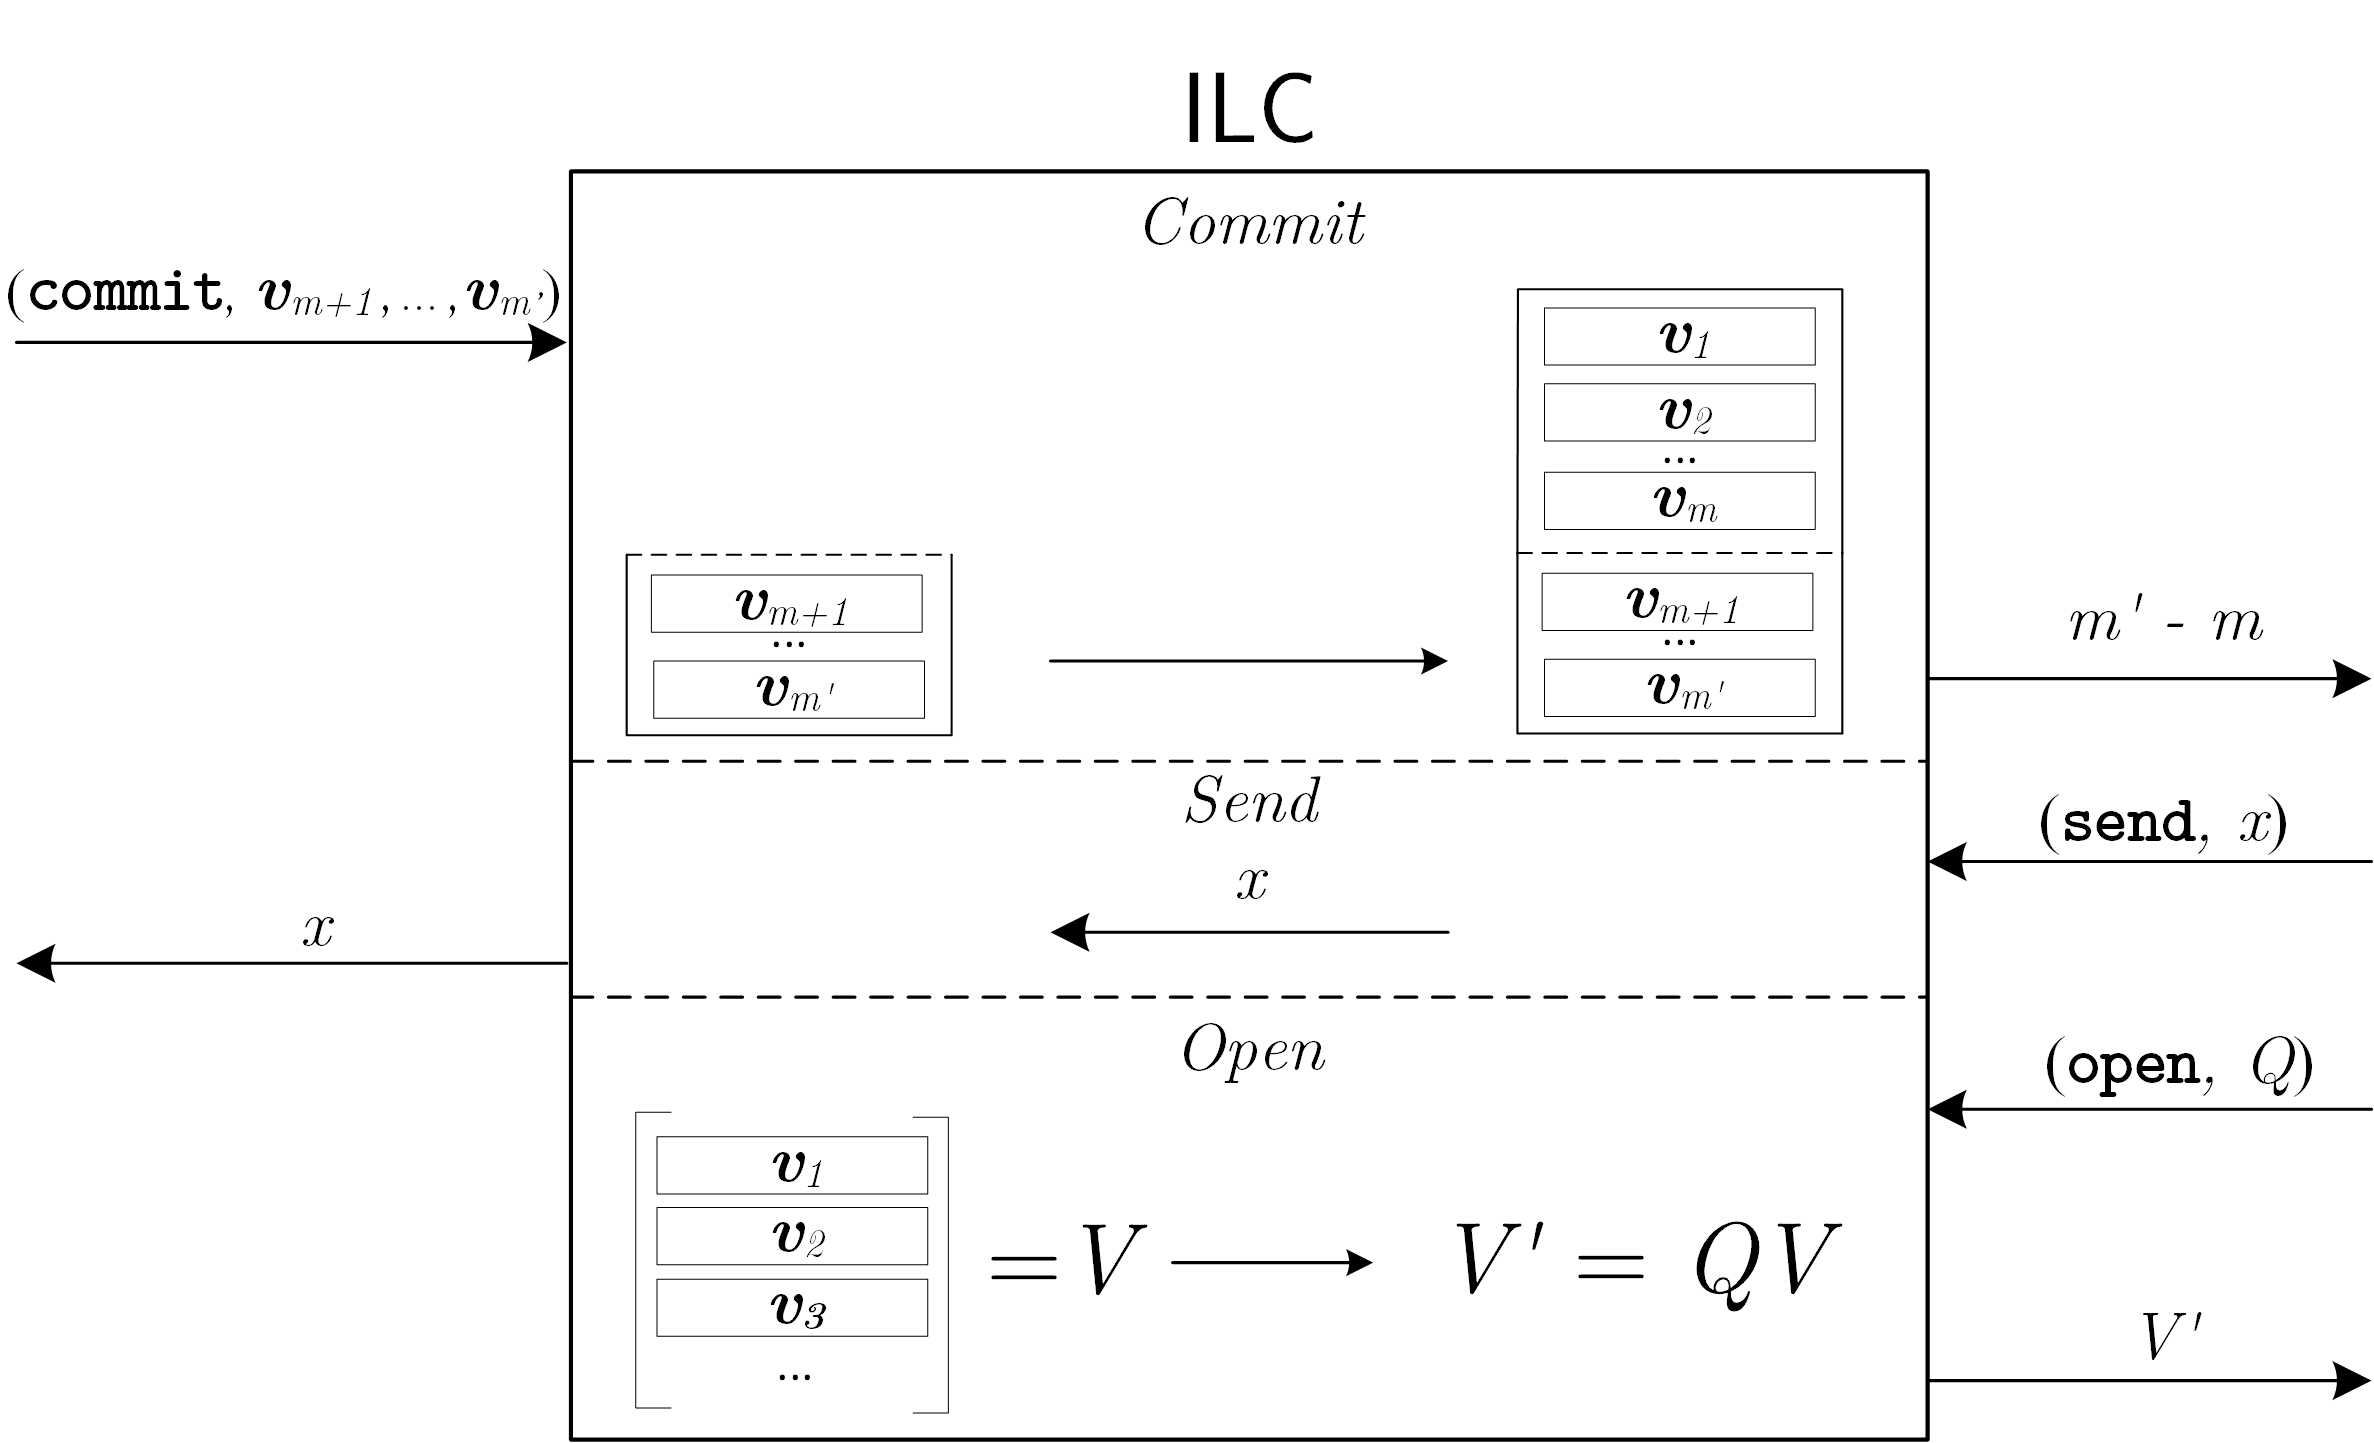
\includegraphics{ILC2-shrink.png}} }&$\V_{\ILC~}$\\
&& \\&&\\&&\\&&\\&&\\&&\\&&\\&&\\&&\\&&\\&&\\
&&\\&&\\
\end{tabular}}\caption{Description of the $\ILC~$ channel.}\label{ILCSyntaxFigure11}
\end{figure}

In a proof system over the \ILC\ channel, sequences of \ILCcommit, \ILCsend\ and \ILCopen\ and \ILCcheck\ queries could alternate in an arbitrary order. We call a proof system over the \ILC\ channel \emph{non-adaptive} if the verifier only makes one \emph{open} query and then immediately one \emph{check} query to the \ILC\ channel, before terminating his interaction with the channel, %only sends one \emph{open} message and it is the last one,
 otherwise we call it \emph{adaptive}. Although adaptive proof systems are allowed by the model, in this paper we will only consider non-adaptive \ILC\ proof systems to simplify the exposition. In non-adaptive \ILC\ proof systems with vectors of length $\sizevect$, the verifier will produce two query matrices, $Q$ for the \ILCopen\ query and $Q$ for the \ILCcheck\ query. 

In fact, in our protocols, we will allow the prover to commit to vectors of \emph{several different fixed lengths} $\sizevect_1,\ldots,\sizevect_r$, which will be specified at the beginning of the protocol. This is easily formalised by defining a new communication channel, giving the prover and verifier access to $r$ copies of different \ILC\ channels of lengths $\sizevect_1,\ldots,\sizevect_r$. For the new channel, the \ILCcommit\ command on vectors $\vec{v}_1,\ldots,\vec{v}_m$ separates the vectors into sets of vectors of lengths $\sizevect_1,\ldots,\sizevect_r$, and commits to the set of vectors of length $\sizevect_i$ using the $i$th \ILC\ channel on vectors of length $\sizevect_i$. The \ILCsend\ command for the new channel simply takes the verifier's message and sends it to each of the $r$ \ILC\ channels using their own \ILCsend\ command. For the \ILCopen\ and \ILCcheck\ commands for the new channel, the verifier's queries take the form $Q = (Q_1,\ldots,Q_r)$, where each $Q_i$ is a query matrix for the $i$th \ILC\ channel. The new channel returns the responses of all of the \ILC\ queries to the verifier. Such a channel will be referred to as an \ILC\ channel for vectors of several fixed lengths, and will be specified simply by including multiple vector lengths in $\crs_{\ILC~}$ rather than just one.

Alternatively, we can easily incorporate vectors of different lengths into the model by padding all vectors with zeroes until they are the same length as the longest vector. This will have no impact on the asymptotic efficiency of our protocols. Some of our \ILC\ protocols require single values to be committed as well as vectors. 

We remind the reader that \ILC\ proof systems are different from linear interactive proofs considered in \cite{BitanskyCIPO13}. In linear interactive proofs both the prover and verifier send vectors of field elements, but the prover can only send linear (or affine) transformations of the verifier's previously sent vectors. However, for our constructions it is important that the prover can compute on field elements received by the verifier and for instance evaluate polynomials.

We say a proof system is \emph{public coin} if the verifier's messages to the communication channel are chosen uniformly at random and independently of the actions of the prover, i.e., the verifier's messages to the prover correspond to the verifier's randomness $\rho$.

We will model our zero-knowledge proofs using ternary relations $\R$ consisting of tuples $(\crs, \stm,\wit)$. Then, we can define a language $\LL_\R \subset \{0,1\}^*$ as follows.
\[ \LL_\R=\{(\crs,\stm)|\exists \wit: (\crs,\stm,\wit)\in \R\} \]
Intuitively speaking, this is the collection of statements which are `true', and for which the verifier should output one after running the protocol with an honest prover. The languages $\LL_\R$ are decidable in polynomial time. The first item in the tuple, $\stm$ is the \emph{instance} and represents what the prover wants to prove. The second, $\wit$, is the prover's secret \emph{witness} that $(\crs,\stm)\in\LL_\R$. The last is the \emph{common reference string} $\crs$ containing the setup information required for the protocol. Typically, $\crs$ will specify the security parameter $\sep$, perhaps implicitly through its length, and may also contain other parameters used for specifying the specific relation, e.g. a description of a field. Typically, $\crs$ will also contain parameters that do not influence membership of $\R$ but may aid the prover and verifier, for instance, a description of an encoding function that they will use.

The protocol $(\KK,\mathcal{P},\mathcal{V})$ is called a \emph{proof of knowledge} over communication channel $\overset{\textnormal{chan}}{\longleftrightarrow}$ for relation $\R$ if it has perfect completeness and computational knowledge soundness as defined below.

\begin{definition}[Perfect Completeness]
The proof is \emph{perfectly complete} if for all PPT adversaries $\mathcal{A}$
$$\Pr \left[ \begin{array}{c} \crs\gets \KK(1^\sep); (u,w) \leftarrow \mathcal{A}(\crs): \\
(\crs,u,w)\notin \R ~\vee~ \langle \mathcal{P}(\crs,u,w)\overset{\textnormal{chan}}{\longleftrightarrow}\mathcal{V}(\crs,u)\rangle=1 \end{array}\right] =1.$$
\end{definition}

\begin{definition}[Knowledge soundness]
A public-coin proof system has \emph{computational (strong black-box) knowledge soundness} if for all DPT $\Po^*$ there exists an expected PPT extractor $\E$ such that for all PPT adversaries $\A$
$$\Pr\left[\begin{array}{c} \crs\gets \KK(1^\sep);(\stm,s) \gets \mathcal{A}(\crs); \wit\gets \E^{\langle \Po^*(s)\overset{\textnormal{chan}}{\longleftrightarrow}\V(\crs,\stm)\rangle}(\crs,\stm):\\ b=1 ~\wedge~ (\crs,\stm,\wit)\notin \R \end{array}\right]\approx 0.$$ 
Here the oracle $\langle \Po^*(s)\overset{\textnormal{chan}}{\longleftrightarrow}\V(\crs,\stm)\rangle$ runs a full protocol execution and if the proof is successful it returns a transcript of the prover's communication with the channel. The extractor $\E$ can ask the oracle to rewind the proof to any point in a previous transcript and execute the proof again from this point on with fresh public-coin challenges from the verifier. We define $b\in \{0,1\}$ to be the verifier's output in the first oracle execution, i.e., whether it accepts or not, and we think of $s$ as the state of the prover. The definition can then be paraphrased as saying that if the prover in state $s$ makes a convincing proof, then we can extract a witness.

If the definition holds also for unbounded $\mathcal{P}^*$ and $\A$ we say the proof has {\em statistical knowledge soundness}. 

If the definition of knowledge soundness holds for a non-rewinding extractor, i.e., a single transcript of the prover's communication with the communication channel suffices, we say the proof system has knowledge soundness with {\em straight-line extraction}. 
\end{definition}
\noindent
Another way to define a proof of knowledge follows Groth and Ishai~\cite{GrI08} who borrowed the term witness-extended emulation from Lindell~\cite{Lin03}. Informally, their definition says that given an adversary that produces an acceptable argument with some probability, there exists an emulator that produces a similar argument with the same probability together with a witness $w$. Note that the emulator is allowed to rewind the prover and verifier's interaction to any previous move.

\begin{definition}[Witness-extended emulation]
$(\mathcal{P},\mathcal{V})$ has {\em statistical witness-extended emulation} if for all deterministic polynomial time $\mathcal{P}^*$ there exists an expected polynomial time emulator $\mathcal{E}$ such that for all interactive adversaries $\mathcal{A}$
\begin{align*}
& \Pr \Big{[}(u,s) \leftarrow\mathcal{A}(1^\sep); tr \leftarrow \langle \mathcal{P}^*(u,s), \mathcal{V}(u)\rangle: \mathcal{A}(tr)=1 \Big{]}\\
\approx \ & \Pr \left[ \begin{array}{l} (u,s) \leftarrow \mathcal{A}(1^\sep); (tr,w) \leftarrow \mathcal{E}^{ \langle \mathcal{P}^*(u,s), \mathcal{V}(u) \rangle } (u): \\ \mathcal{A}(tr)=1 \text{\emph{ and if }} tr \text{\emph{ is accepting then }} (u,w) \in R \end{array} \right]
\end{align*}
where the oracle called by $\mathcal{E}^{\langle \mathcal{P}^*(u,s), \mathcal{V}(u)\rangle}$ permits rewinding to a specific point and resuming with fresh randomness for the verifier from this point onwards.
\end{definition}
\noindent
In the definition, $s$ can be interpreted as the state of $\mathcal{P}^*$, including the randomness. So, whenever $\mathcal{P}^*$ is able to make a convincing argument when in state $s$,  $\mathcal{E}$ can extract a witness. Witness Extended Emulation implies Knowledge Soundness \cite{dissertation}.

We will construct public-coin proofs that have special honest-verifier zero-knowledge. This means that if the verifier's challenges are known, or even adversarially chosen, then it is possible to simulate the verifier's view without the witness.  In other words, the simulator works for verifiers who may use adversarial coins in choosing their challenges but they follow the specification of the protocol as an honest verifier would. 
\begin{definition}[Special Honest-Verifier Zero-Knowledge]
The proof of knowledge is \emph{computationally special honest-verifier zero-knowledge (SHVZK)} if there exists a PPT simulator $\mathcal{S}$ such that for all stateful interactive PPT adversaries $\mathcal{A}$ that output $(u,w)$ such that $(\crs,u,w)\in R$ and randomness $\rho$ for the verifier
\begin{eqnarray*}
&&\Pr \left[ \begin{array}{c}\crs\gets \KK(1^\sep);(u, w, \rho) \leftarrow\mathcal{A}(\crs); \\
\viewV\leftarrow \langle \mathcal{P}(\crs,u,w)\overset{\textnormal{chan}}{\longleftrightarrow} \V(\crs,u;\rho)\rangle: \A(\viewV)=1\end{array} \right]\\
&\approx &\Pr \left[ \crs\gets \KK(1^\sep);(u, w, \rho) \leftarrow\mathcal{A}(\crs); \viewV\leftarrow \mathcal{S}(\crs,u,\rho): \mathcal{A}(\viewV)=1\right].
\end{eqnarray*}

We say the proof is \emph{statistically SHVZK} if the definition holds also against unbounded adversaries, and we say the proof is \emph{perfect SHVZK} if the probabilities are exactly equal.
\end{definition}


\heading{\bf From Honest-Verifier to General Zero-Knowledge}
Honest-verifier zero-knowledge only guarantees the simulator works for verifiers following the proof system specifications. It might be desirable to consider general zero-knowledge where the simulator works for arbitrary malicious verifiers that may deviate from the specification of the proof. However, honest-verifier zero-knowledge is a first natural stepping stone towards efficient zero-knowledge proofs. %and it depends on the situation how you would want to proceed to get full zero-knowledge. 
 We recall that our proofs are public coin, which means that the verifier's messages are chosen uniformly at random and independently from the messages received from the verifier. Below we recall few options to obtain general zero-knowledge proofs from a public-coin SHVZK proof. All these transformations are very efficient in terms of computation and communication such that the efficiency properties of our special honest-verifier zero-knowledge protocols are preserved. 

In the Fiat-Shamir transform \cite{FiatShamir} the verifier's challenges are computed using a cryptographic hash function applied to the transcript up to the challenge. The Fiat-Shamir transform is more generally used to turn a public-coin proof into a non-interactive one. Since interaction with the verifier is no longer needed, general zero-knowledge is immediately achieved. The drawback of the Fiat-Shamir transform is that security is usually proved in the random oracle model \cite{bellarerogaway} where the hash function is modelled as an ideal random function.% truly random message digests.

Other transformations such as \cite{Damgard2000,MP03,GoldreichSV98} have already been discussed.
%
%Assuming a common reference string and relying on trapdoor commitments, Damg{\aa}rd \cite{Damgard2000} gave a transformation yielding concurrently secure protocols for $\Sigma$-Protocols. The transformation can be optimized~\cite{dissertation} using the idea that for each public-coin challenge $x$, the prover first commits to a value $x'$, then the verifier sends a value $x''$, after which the prover opens the commitment and uses the challenge $x=x'+x''$. The coin-flipping can be interleaved with the rest of the proof, which means the transformation preserves the number of rounds and only incurs a very small efficiency cost to do the coin-flipping for the challenges. 
%
%If one does not wish to rely on a common reference string for security, one can use a private-coin transformation where the verifier
%does not reveal the random coins used to generate the challenges sent to the prover (hence the final protocol is no longer public coin).
%One example is the Micciancio and Petrank \cite{MP03} transformation (yielding concurrently secure protocols) while incurring a small overhead of $\omega(\log{\lambda})$ with respect to the number of rounds as well as the computational and communication cost in each round. % where $\lambda$ is the security parameter and $\omega(\log{\lambda})$ is independent of the complexity of the original protocol. 
%The transformation preserves the soundness and completeness errors of the original protocol; however, it does not preserve statistical zero-knowledge as the obtained protocol only has computational zero-knowledge. 
%
%There are other public-coin transformations to general zero-knowledge e.g.~Goldreich et al.~\cite{GoldreichSV98}. The transformation relies on a random-selection protocol between the prover and verifier to specify a set of messages and restricting the verifier to choose challenges from this set. This means to get negligible soundness error these transformations require $\omega(1)$ sequential repetitions so the round complexity goes up. 
%
\section{Arithmetic Circuits}\label{sec:AC}

Arithmetic circuits are a model for algebraic computation over fields. An arithmetic circuit consists of addition and multiplication gates. Our satisfiability arguments consider arithmetic circuits described as a list of multiplication gates together with a set of linear consistency equations relating the inputs and outputs of the gates. 
%
In this section, we show how to reduce an arbitrary arithmetic circuit to this format.

\begin{definition} An arithmetic circuit over a field $\F_p$ and variables $(A_1,\ldots,A_m)$ is a directed acyclic graph whose vertices are called gates. Gates of in-degree 0 are inputs to the circuit and labelled with some $A_i$ or a constant field element. All other gates are labelled $+$ or $\times$.
\end{definition}

Given field elements $a_i \in \F$, we compute the arithmetic circuit by labelling the inputs with these field elements, then by taking gates whose inputs are all labelled with field elements, applying the operation on the gate to the inputs, writing the answer on the output, and repeating this process until all gates have been labelled with output field elements.

We may consider fan-in 2 circuits, in which case all of the $+$ and $\times$ gates have in-degree 2, or arbitrary fan-in circuits. We consider circuits with arbitrary fan-out, in which case all of the $+$ and $\times$ gates have unbounded out-degree.

Arithmetic circuits can be measured in various ways. The size of an arithmetic circuit is the number of gates in the circuit. This can be further split into the number of addition gates and the number of multiplication gates. The depth of a circuit is the length of the longest path beginning from any circuit input. It is easy to see that arithmetic circuits compute polynomial functions of their inputs, and the degree of the arithmetic circuit is the total degree of the polynomial that it computes.

Arithmetic circuits can be described alternatively as a list of multiplication gates with a collection of linear consistency equations relating the inputs and outputs of the gates. Our zero-knowledge protocols for circuit satisfiability use circuits in this form. Any circuit described as an acyclic graph can be efficiently converted into the alternative description.

At a high level, we transform an arithmetic circuit into two kinds of equations. 
Multiplication gates are directly represented as equations of the form $a\cdot b=c$, where $a,b,c$ represent the left, right and output wires. We will arrange these values in matrix form producing a Hadamard matrix product. This process will lead to duplicate values, when a wire is the output of one multiplication gate and the input of another, or when it is used as input multiple times. We keep track of this by using a series of linear constraints. For example, if the output of the first multiplication gate is the right input of the second, we would write $c_1 - b_2 = 0$.

We also add linear constraints representing the addition and multiplication by constant gates of the circuit. We then rewrite those equations so that the only wires that are referenced in the equations are those linked to (non-constant) multiplication gates. %This is always possible if we allow for some preprocessing of the initial circuit. 
We now describe this process.

\subsection{Reduction of Circuit Satisfiability to a Hadamard Matrix Product and Linear Constraints.}
We consider an arithmetic circuit containing $N=mn$ multiplication gates over a field $\F$. Without loss of generality, we assume that the circuit has been pre-processed as in the next section, so that the input and the output wires feed into and go out from multiplication gates only.
We number the multiplication gates from 1 to $N$ and we arrange the inputs and outputs of these gates into three $m\times n$ matrices $A,B$ and $C$ such that the $(i,j)$ entries of the matrices correspond to the left input, right input and output of the same multiplication gate.

As shown in \cite{BootleCCGP16}, an arithmetic circuit can be described as a system of equations in the entries of the above matrices. The multiplication gates define a set of $N$ equations 
\begin{equation}\label{eq1:product}
A \circ B = C
\end{equation}
where $\circ$ is the Hadamard (entry-wise) product. 
%
The circuit description also contains constraints on the wires between multiplication gates. %The output of one multiplication gate might feed into a combination of addition gates and multiplication by constant gates yielding one or more inputs to other multiplication gates. 
Denoting the rows of the matrices $A,B,C$ as
\begin{align*}\vec{a}_ {i}=(a_{i,1},\ldots,a_{i,n})&& \vec{b}_ {i}=(b_{i,1},\ldots,b_{i,n})&&\vec{c}_ {i}=(c_{i,1},\ldots,c_{i,n})&& \text{for }  i \in \{1,\ldots,m\}\end{align*}
these constraints can be expressed as $Q<2N$ linear equations of inputs and outputs of multiplication gates of the form
\begin{equation}\label{eq1:consistency}
\sum_{i=1}^m \vec{a}_{i} \cdot \vec{w}_{q,{a,i}}+\sum_{i=1}^m \vec{b}_{i} \cdot \vec{w}_{q,{b,i}}+\sum_{i=1}^m \vec{c}_{i} \cdot  \vec{w}_{q,{c,i}}=K_{q} \quad \text{ for } q \in\{1,\ldots,Q\}
\end{equation}
for constant vectors $\vec{w}_{q,{a,i}},\vec{w}_{q,{b,i}},\vec{w}_{q,{c,i}}$ and scalars $K_{q}$.

For example, suppose that the circuit contains a single addition gate, with $a_{1,1}$ and $a_{1,2}$ as inputs, and $b_{1,1}$ as output. In this case, $Q=1$ and we would set $\vec{w}_{1,a,1} = (1,1,0,\ldots,0)$, $\vec{w}_{1,b,1} = (-1,0,\ldots,0)$, and all other $\vec{w}$ vectors would be set to $\vec{0}$. Then~\eqref{eq1:consistency} would simply read
$$ a_{1,1} + a_{1,2} - b_{1,1} = 0$$
to capture the constraint imposed by the addition gate.

In total, to capture all multiplications and linear constraints, we have $N+Q$ equations that the wires must satisfy in order for the circuit to be satisfiable. %We can combine the equations into a polynomial of degree $N+Q$ in an indeterminate $Y$ such that the circuit is satisfiable if and only if the polynomial is identically 0.

\subsection{Preprocessing Arithmetic Circuits for Arguments}\label{sec:preprocAC}

We show how to remove addition and multiplication-by-constant gates  from an arithmetic circuit $A$, and replace them with bilinear consistency equations on the inputs and outputs of the remaining gates, such that satisfiability of the equations is equivalent to satisfiability in the original circuit.

 Let $B$ be the sub-circuit of $A$ containing all wires and gates before a multiplication gate, with $m$ input wires and $n$ output wires. Label the $m$ inputs of $B$ with the unit vectors $\vec{e}_i=(0,\ldots,1,\ldots,0)$ of length $m$. For every addition gate with inputs labelled as $\vec{x},\vec{y}$, label the output wire as $\vec{x}+\vec{y}$. For every multiplication-by-constant gate with inputs $\vec{x}$ and constant $c$ label the output with $c\vec{x}$. By proceeding inductively, the $n$ outputs of $B$ are now labelled with vectors of length $m$ representing them as linear combinations of the inputs.

This requires at most $m\left| B \right|$ arithmetic operations. Note however that all outputs of $B$ are linear combinations of the inputs, and that $B$ can be written with $n(2m-1)$ fan-in 2 gates in such a way that the consistency equations can be trivially read off from the circuit description. More specifically, a linear combination $\sum_{i=1}^m a_i x_i$ can be produced using $m$ multiplication-by-constant gates and $m-1$ addition gates to add the answers together.

We can now remove the gates of $B$ from $A$. We also remove any multiplication gates whose inputs are the inputs of the new circuit. Now we simply repeat the process of finding consistency equations until we have considered the whole of~$A$. In Figure~\ref{fig:digraph} there is an example of a circuit together and the corresponding consistency equations.



The first (input) and final (output) sub-circuits require additional processing. We show how to do this for the output sub-circuit. The input sub-circuit is very similarly handled.

Let $B$ be the output sub-circuit. Write $(a_1,\ldots,a_m)=\vec{a}$ for the input wires of $B$ and $(b_1,\ldots,b_n)=\vec{b}$ for the output wires. Without loss of generality, we may ignore variable output wires. By construction of $B$, each output $b_i$ is of the form $\sum_{i=1}^n q_{ij}a_j+p_i$, with consistency equations obtained as above. We write this in terms of an $m\times n$ matrix $\mathsf{Q}$ and a column vector $\vec{p}$ of size $m$, namely
$$\vec{b} = \mathsf{Q} \vec{a}+ \vec{p}.$$
%
Let $r$ be the rank of $\mathsf{Q}$. We convert $\mathsf{Q}$ into reduced row echelon form $\mathsf{R}$, writing
$$\vec{b''}=\mathsf{R}\vec{a}.$$

By the properties of reduced row echelon form, after relabelling the $a_i$ and permuting the columns of $\mathsf{R}$ to match, we have that $b''_i=a_i + \sum_{j=l+1}^m r_{ij} a_j$ for $1\leq i\leq l$. Therefore, we may consider $a_{l+1},\ldots,a_m$ as free wires and express other $a_i$ as linear functions of these wires plus constants.

Note that if $b''_i\neq 0$ for some $i>l$, the circuit can never be satisfied anyway. However, assuming that our statement is a satisfiable circuit, with a witness consisting of satisfying wire values, this never occurs. Then the original circuit is satisfied if and only if the $a_i$ values satisfy the consistency equations.

If $\mathsf{Q}$ is an $m\times n$ matrix then it can be converted into reduced row echelon form using $O(\mathrm{max}(m,n) mn)$ operations. It is trivial that $m\leq 2\left| B \right|$ and $n\leq \left| B \right|$. This gives an upper bound of $O(\left| B \right|^3)$ computation for the output sub-circuit. 
%
Note that this is often a large over-estimate; this upper bound occurs for circuits of depth 1 where inputs feed into distinct gates. For circuits of large depth, where the same input is fed into several gates, the upper bound will definitely not be reached. %Recall that the circuit $B$ computes a linear map and can be written so that $\left| B \right| = O(mn)$. Then the computational cost is $O(\mathrm{max}(m,n) \left| B \right|)$.

The case of the input sub-circuit is very similar, except that we take the transpose of the matrix.

\begin{figure}
\centering
\scalebox{0.7}{
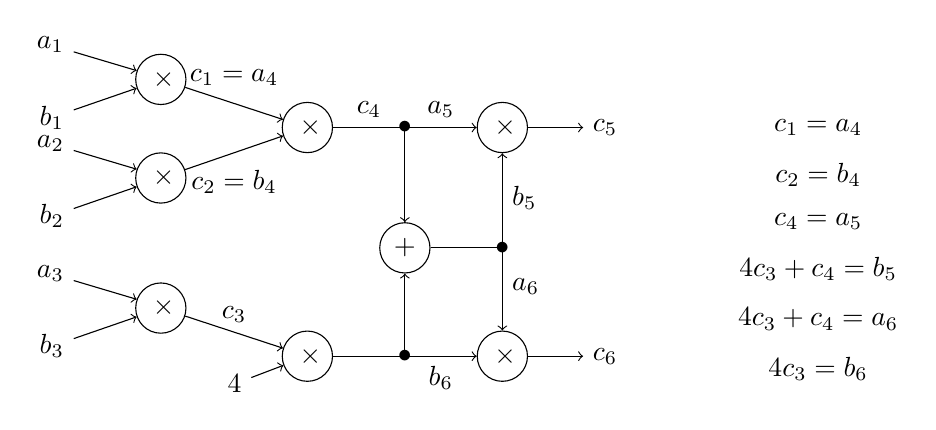
\begin{tikzpicture}[gate/.style={circle,draw,text width=0.2 cm, align=center}]
%level 1

\node[gate] (m1) {$\times$};
\node[above left= 0.1 cm and 0.8 cm of m1.160] (a1) {$a_1$};
\node[below left= 0.1 cm and 0.8 cm of m1.200] (b1) {$b_1$};
\draw[->] (a1) -- (m1.160);
\draw[->] (b1) -- (m1.200);


\node[gate, below = 0.6 cm of m1] (m2) {$\times$};

\node[ above left=0.1 cm and 0.8 cm of m2.160] (a2) {$a_2$};
\node[below left=0.1 cm and 0.8 cm of m2.200] (b2) {$b_2$};
\draw[->] (a2) -- (m2.160);
\draw[->] (b2) -- (m2.200);

\node[gate, below = of m2] (m3) {$\times$};

\node[above left=0.1 cm and 0.8 cm of m3.160,font=\bfseries] (a3) {$a_3$};
\node[below left=0.1 cm and 0.8 cm of m3.200,font=\bfseries] (b3) {$b_3$};
\draw[->] (a3) -- (m3.160);
\draw[->] (b3) -- (m3.200);




%level 2
\node[gate,below right= 0.15 cm and 1.4 cm of m1] (m4) {$\times$};

\node[gate,below right= 0.15 cm and 1.4 cm of m3] (cm1) {$\times$};
\node[ below right = 0.7 of m3] (cc) {$4$};


\draw[->] (m1) -- (m4) node [midway, above =0.1 cm  ] {$c_1=a_4$};
\draw[->] (m2) -- (m4) node [midway, below=0.1 cm] {$c_2=b_4$};

\draw[->] (m3) -- (cm1) node [midway, above] {$c_3$};
\draw[->] (cc) -- (cm1);


%level 3

\node[right = 0.7 of m4 ] (dot1) {$\bullet$ } ;
\node[gate, below = of dot1 ] (a1) {+};
\node[right = 0.7 of cm1] (dot2) {$\bullet$};

\draw[->] (dot1.center) -- (a1);
\draw[->] (dot2.center) -- (a1);


%level 4
\node[gate, right = 0.7 cm of dot1 ] (m5) {$\times$};
\node[ right =  0.7 cm of a1 ] (dot3) {$\bullet$};
\node[gate, right =0.7 cm  of dot2 ] (m6) {$\times$};
%\node[right = of m4 ] (dot1) {$\bullet$ } ;

%\node[right = of cm1 ] (dot2) {$\bullet$};


\draw[->] (m4) -- (m5) node [near start, above] {$c_4$} node [near end, above] {$a_5$};
\draw[->] (cm1) -- (m6) node [near end, below] {$b_6$};
\draw (a1) -- (dot3.center) ;


\draw[<->] (m5) -- (m6) node [near start, right ] {$b_5$} node [near end, right] {$a_6$};


%level 5

\node[ right = 0.7 cm of m5 ] (out1) {$c_5$};
\node[ right = 0.7 cm  of m6 ] (out2) {$c_6$};
\draw[->] (m5) -- (out1) ;
\draw[->] (m6) -- (out2) ;

%level 6
\node[ right =3 cm of m5] (eq) {$c_1=a_4$};
\node[below =0.1 cm of eq] (eq1) {$c_2=b_4$};
\node[below =0.1 cm of eq1] (eq2) {$c_4=a_5$};
\node[below =0.1 cm of eq2] (eq3) {$4c_3+c_4=b_5$};
\node[below =0.1 cm of eq3] (eq4) {$4c_3+c_4=a_6$};
\node[below =0.1 cm of eq4] (eq5) {$4c_3=b_6$};


\end{tikzpicture}
}
\vspace{-.2cm}
\caption{A simple arithmetic circuit, and the corresponding consistency equations. The first sub-circuit contains the wires $a_1,b_1,c_1,a_2,b_2,c_2,a_3,a_3,c_3$. The second sub-circuit contains the wires $c_1,a_4, c_2,b_4,c_4, c_5,c_6$. The third sub-circuit $B$ contains the wires $c_3,c_4,a_5,b_5,a_6$.}
\label{fig:digraph} 
\end{figure}

\section{Commitment Schemes}
\label{sec:BComDef}
A non-interactive commitment scheme allows a sender to commit to a secret message and later reveal the message in a verifiable way. Here we are interested in commitment schemes that take as input an arbitrary length message so the message space is $\{0,1\}^*$. A commitment scheme is defined by a pair of PPT algorithms $(\ComSetup,\ComCommit)$.
\begin{description}
\item [$\ComSetup(1^\sep)\to ck$:]
Given a security parameter, this returns a commitment key $ck$.
\item [$\ComCommit_{ck}(m)\to \Co$:] Given a message $m$ from a message space $\mathcal{M}_{ck}$, this picks randomness $r\gets \mathcal{R}_{ck}$, from a randomness space, and computes a commitment $\Co=\ComCommit_{ck}(m;r) \in \mathcal{C}_{ck}$. 
\end{description}
A commitment scheme must be \emph{binding} and \emph{hiding}. The binding property means that it is infeasible to open a commitment to two different messages, whereas the hiding property means that the commitment does not reveal anything about the committed message. 
\begin{definition} [Binding]
A commitment scheme is \emph{computationally binding} if for all PPT adversaries $\A$
$$ \Pr\left[
\begin{array}{c}
ck \asn \ComSetup(1^\sep);~ (m_0,r_0,m_1,r_1)\asn \A(ck): \\
m_0\neq m_1 ~\wedge~ \ComCommit_{ck}(m_0;r_0)=\ComCommit_{ck}(m_1;r_1)
\end{array}
\right] \approx 0.
$$
If this holds also for unbounded adversaries, we say the commitment scheme is \emph{statistically binding}.
\end{definition}
\begin{definition} [Hiding]
A commitment scheme is \emph{computationally hiding} if for all PPT stateful adversaries $\A$
$$ \Pr\left[\begin{array}{c}ck \asn \ComSetup(1^\sep);~(m_0,m_1)\asn \A(ck);~b \gets \{0,1\};~ \\
\Co\gets \ComCommit_{ck}(m_b):~\A(\Co)=b
\end{array}\right] \approx \frac{1}{2},$$
where $\A$ outputs messages of equal length $|m_0|=|m_1|$.
If the definition holds also for unbounded adversaries, we say the commitment scheme is \emph{statistically hiding}.
\end{definition}

Suppose further that $(\mathcal{M}_{ck},\cdot)$, $(\mathcal{R}_{ck},\circ)$ and $(\mathcal{C}_{ck},\oplus)$ are groups.
\begin{definition}[Homomorphic Commitment Scheme]
We call the commitment scheme homomorphic if $\ComCommit:\mathcal{M}_{ck}\times\mathcal{R}_{ck}\to \mathcal{C}_{ck}$ is a group-homomorphism, i.e. 
$$\ComCommit(m \cdot m';r\circ r')=\ComCommit(m;r)\oplus \ComCommit(m';r')$$
\end{definition}

\section{Error-Correcting Codes}\label{sec:LC}
A \emph{code} over an alphabet $\Sigma$ is a subset $\codeset\subseteq \Sigma^n$. A code $\codeset$ is associated with an encoding function $E_\codeset:\Sigma^k\to \Sigma^n$ mapping messages of length $k$ into \emph{codewords} of length $n$.
We assume there is a setup algorithm ${\text{Gen}}_{\preECC}$ which takes as input a finite field $\F$ and the parameter $k \in \N$, and outputs an encoding function $E_\codeset$.

We use error-correcting codes as part of our compilation from \ILC\ protocols to argument systems based on collision-resistant hash-functions. We restrict our attention to $\F$-\emph{linear codes} for which the alphabet is a finite field $\F$, the code $\codeset$ is a $k$-dimensional linear subspace of $\F^n$, and $E_\codeset$ is an $\F$-linear map. The \emph{rate} of the code is defined to be $\frac{k}{n}$. The \emph{Hamming distance} between two vectors $\vec{x},\vec{y} \in \F^n$ is denoted by $\hamdist(\vec{x},\vec{y})$ and corresponds to the number of coordinates in which $\vec{x},\vec{y}$ differ. The \emph{(minimum) distance} of a code is defined to be the minimum Hamming distance $\minhamdist$ between distinct codewords in $\codeset$. %, and the \emph{relative distance} $\relmindist=\frac{\minhamdist}{n}$. 
We denote by $[n,k,\minhamdist]_\F$ a linear code over $\F$ with length $n$, dimension $k$ and minimum distance $\minhamdist$. The \emph{Hamming weight} of a vector $\vec{x}$ is $\hamweight(\vec{x})=|\{i \in [n]: \vec{x}_i \neq 0\}|$.

%The Hamming distance satisfies the triangle inequality, $\hamdist(\vec{a},\vec{c})\leq \hamdist(\vec{a},\vec{b})+\hamdist(\vec{b},\vec{c})$ as well as $\hamdist(\vec{a}+\vec{c},\vec{b}+\vec{d})\leq \hamdist(\vec{a},\vec{b})+\hamdist(\vec{c},\vec{d})$. 

To get good results when compiling , we will use families of linear codes achieving asymptotically good parameters. More precisely, we require codes with linear length, $n=\Theta(k)$, and linear distance, $\minhamdist=\Theta(k)$, in the \emph{dimension} $k$ of the code.
We recall that random linear codes achieve with high probability the best trade-off between distance and rate. However, in this work we are concerned with the computational efficiency of the encoding procedure and random codes are not known to be very efficient. The reader can keep Reed-Solomon codes in mind for concrete instantiations, as these as simple, satisfy all of the necessary requirements, and are practically efficient as well as asymptotically.
% !TEX root = ..\Main.tex
\chapter{Cryptographic Assumptions and Concrete Commitment Schemes}
\label{chapterlabel:Cryptographic-Assumptions}

Zero-knowledge protocols are often built based on cryptographic assumptions stating that various mathematical problems cannot be solved efficiently. In this thesis, we show that efficient zero-knowledge proofs and arguments can be built easily based on two different cryptographic assumptions: the discrete logarithm assumption, and the existence of collision resistant hash functions. Here, we formally define both of these assumptions.

We define cryptographic assumptions relative to instance generators $\instancegen$.

\section{The Discrete Logarithm Assumption}

The discrete logarithm assumption is a computational hardness assumption relative to a given group $\G$. Given two group elements $g$ and $h$ in $\G$, the discrete logarithm problem is to compute an integer $k$ such that $g^k = h$ in $\G$.

The discrete logarithm problem has been extensively studied. It forms the basis for cryptosystems and commitments, such as the ElGamal encryption scheme and the Pedersen commitment scheme. Researchers have also devised algorithms to solve the discrete logarithm problem, some of which work for any group, and some of which work for particular choices of group.

\paragraph{Formal Definition}

Let $\instancegen$ be a probabilistic, polynomial time algorithm that on input $1^\sep$ returns a description $\instance = (\G,\DLOGprime,g)$ of a group $\G$ of prime order $\DLOGprime$, with a generator $g$. Assume that the group has associated polynomial time algorithms for computing group operations and deciding membership.

We say that the discrete logarithm assumption holds relative to $\instancegen$ if for all probabilistic polynomial time adversaries $\adversary$ and all $\sep \in \N$,
$$ \Pr \left[ \instance = (\G,\DLOGprime,g) \gets \instancegen(1^\sep); x \gets \Z_\DLOGprime; h := g^x : \adversary(\instance,h)=x \right] \approx 0 $$

\paragraph{Commitment Scheme} The Pedersen commitment scheme \cite{Pedersen91} is a well-known commitment scheme based on the discrete logarithm assumption. The original commitment scheme allows a committer to commit to a single element, but is easily generalised to a commitment scheme for multiple elements, shown in Figure \ref{alg:com:pedersen}. Here, the message space is $\Z_p^n$ and the randomness space is $\Z_p$. Commitments lie in $\Gr$. The binding property comes from the discrete logarithm assumption, and the hiding property from the fact that $r$ is chosen uniformly at random, so that commitments are distributed as random group elements.

Perhaps suprisingly, a Pedersen commitment on a message of length $n$ can be computed using $O(n / \log n)$ group operations rather than the $O(n)$ operations that one might expect, using Pippenger's algorithm. A special case of the algorithm- which is sufficient to obtain our results- is explained in Appendix \ref{appendix:multiexp}.

Pedersen commitments are an attractive choice because they are both succinct, and simple and easy to compute using exponentiation operations on group elements. Our \ILC\ protocols use only arithmetic operations over fields. When instantiated using Pedersen commitments, although the protocols are more complicated, the types of operations required to compute the resulting zero-knowledge proofs are fundamentally the same as those required to compute DSA or ECDSA signatures, with the addition of well-known Fast Fourier transform algorithms to perform some polynomial operations. This should make it extremely easy to produce efficient implementations of our \ILC\ protocols when they are compiled into the discrete logarithm setting.

\begin{figure}[t]
  \caption{Pedersen Commitments}
\label{alg:com:pedersen}
\fbox{\centerline{\small\begin{minipage}[b]{\textwidth}
    \begin{algorithmic}[1]
	\State $\ckgen{1^\sep}{\mlen}$:
	\State $\instance = (\G,\DLOGprime,g) \gets \instancegen(1^\sep)$
	\State Select $\vec{g} \gets \G^{\mlen+1}$
	\State \Return $(\instance,\vec{g})$
    \end{algorithmic}\end{minipage}}}
\fbox{\centerline{\small\begin{minipage}[b]{\textwidth}
    \begin{algorithmic}[1]
	\State $\commit{\vec{m}}{r}$:
	\State Parse $(m_1,\ldots,m_n) = \vec{m}$
	\State Parse $((\G,\DLOGprime,g),(g_1,\ldots,g_n,h)) = \ck$
	\State \Return $h^r \prod_{i=1}^n g_i^{m_i}$
    \end{algorithmic}\end{minipage}}}
\end{figure}

\paragraph{Parameter Choices} The discrete logarithm problem is believed to be difficult when $\G$ is chosen to be a subgroup of the multiplicative group of a prime field, or the group of points of an elliptic curve over a finite field, with large prime order. In order to achieve \sep\ bits of security, different sizes of group are required in each case. Over prime fields, the best known algorithms are based on the general number field sieve \cite{schiro}, and in light of these algorithms, a prime of roughly $\bigo(\sep^3)$ bits is required for $\sep$ bits of security. For most elliptic curves, except those from a few special families, the best algorithms are generic algorithms such as Pollard's rho algorithm, and the order of $\G$ should be approximately $2\sep$ bits.

The binding property of the Pedersen commitment scheme is equivalent to the discrete logarithm assumption, and there is no change in the security of the scheme as $\mlen$ is increased.

The discrete logarithm assumption is well-known, well-examined, and widely used in cryptography. Our protocols rely on the discrete logarithm assumption in groups with prime order $p$. The assumption is believed to hold in suitable subgroups of elliptic-curve groups. The best algorithms for finding discrete logarithms in such elliptic curve groups are still generic algorithms with complexity $\Omega (\sqrt{p})$. For these groups we therefore enjoy lower parameter sizes than protocols based on RSA groups that are subject to sub-exponential attacks.

The discrete logarithm assumption is also believed to hold in well-chosen multiplicative sub-groups of finite fields. Finite fields of prime order should have moduli of $\frac{\lambda^3}{\mathrm{polylog}\lambda}$ bits in order to achieve $\lambda$ bits of security against the best known attacks. This makes protocols communicating large numbers of group elements highly impractical in this setting. Some of our protocols can be tuned so that they only require a constant number of group elements, resulting in much better efficiency when instantiated in finite fields of prime order, since the $\frac{\lambda^3}{\mathrm{polylog}\lambda}$ communication cost can then appear as a constant additive factor rather than a multiplicative one.

\section{The Collision Problem for Hash Functions}

Hash functions are functions which produce a short digest, or hash, of fixed length when applied to an input of arbitrary size. When using hash functions for cryptographic security guarantees, a common requirement is collision resistance. The computational problem here is to generate two different inputs which give the same hash value.

Like Pedersen commitments, hash-based commitments can be extremely simple and efficient to compute. But Pedersen commitments are based on the hardness of the discrete logarithm assumption, and so we expect that a quantum computer running Shor's algorithm would be able to break the binding property of Pedersen commitments, and thus the soundness property of our \ILC\ protocols when compiled in the discrete logarithm setting. However, there is currently no efficient quantum algorithm for breaking the collision-resistance of hash-functions much faster than classical algorithms.

Recent works, most notably \cite{Unruh17}, argue that when made into non-interactive zero-knowledge proofs, certain zero-knowledge proofs are secure in strong threat models against quantum adversaries who are able to perform quantum interactions with the prover or the verifier. Making such arguments about our own protocols is beyond the scope of this thesis, but as they are based on a cryptographic assumption which still resists cryptanalytic attempts by quantum algorithms, it is possible that they could be proved secure against quantum adversaries in the future, or inspire other protocols with quantum security proofs.

\paragraph{Formal Definition.} Collision resistance is properly defined for a family of functions. Let $\HashInLen, \HashOutLen : \N \to \N$ be increasing functions such that $\HashInLen (\sep) > \HashOutLen(\sep)$ for all $\sep \in \N$. Let $\instancegen$ be a probabilistic, polynomial time algorithm that on input $1^{\sep}$ returns a key $s$. Then suppose that there exists a DPT algorithm $\HashFunction$ such that for every $n$ and every $s$, $\HashFunction$ defines a function $\HashFunction : \{0,1\}^{\HashInLen(\sep)} \to \{0,1\}^{\HashOutLen(\sep)}$. Then $(\instancegen,\HashFunction)$ is a fixed-length hash function.

We say that $(\instancegen,\HashFunction)$ is a collision resistant hash function if for all probabilistic polynomial time adversaries $\adversary$ and all $\sep \in \N$,
$$ \Pr \left[ s \gets \instancegen(1^\sep) : \adversary(s) = (x,x'), \ x,x'\in \{0,1\}^{\HashInLen(\sep)}, \HashFunction^s(x) = \HashFunction^s(x') \right] \approx 0 $$

\paragraph{Commitment Scheme.} Halevi and Micali~\cite{HalMic96} show that a collision-resistant hash function gives rise to an efficient and compact statistically hiding commitment scheme. In the following, we tacitly assume that $\HashInLen(\sep)$ is large enough to create a functional commitment scheme. If this is not the case, one can use the Merkle-Damgaard construction or alternatives \cite{Lucks04,NandiP10} used to extend the hash function to a larger input length.

Let $T_{m,n}$ be the space of $m \times n$ Toeplitz matrices over $\Z_2$. This is the collection of matrices such that for each top-left to bottom-right diagonal, every element in the diagonal is equal. Note that $A$ can be described using $m+n-1$ bits.

Figure \ref{alg:com:hash} gives a commitment scheme with message space $\{0,1\}^\HashInLen$, randomness space $\{0,1\}^{O(\HashOutLen)}$ and commitment space $\{0,1\}^{O(\HashOutLen)}$.

\begin{figure}[t]
  \caption{Hash-Based Commitment}
\label{alg:com:hash}
\fbox{\centerline{\small\begin{minipage}[b]{\textwidth}
    \begin{algorithmic}[1]
	\State $\ckgen{1^\sep}{\mlen}$:
	\State Set $L = 6\sep+4$.
	\State $s \gets \crsgen(1^\lambda)$.
	\State \Return $(\HashFunction,s,L)$
    \end{algorithmic}\end{minipage}}}
\fbox{\centerline{\small\begin{minipage}[b]{\textwidth}
    \begin{algorithmic}[1]
	\State $\commit{\vec{m}}{r}$:
	\State Parse $\vec{m}$ as a bitstring.
	\State Parse $\vec{r} \in \{0,1\}^L$.
	\State Compute $\vec{m}' = \HashFunction^s(\vec{m})$.
	\State Select $A \gets T_n$.
	\State Compute $\vec{b} = \vec{m}'-A\vec{r}$.
	\State Compute $y = \HashFunction^s(\vec{r})$.
	\State \Return $(A,\vec{b},y)$
    \end{algorithmic}\end{minipage}}}
\end{figure}

\paragraph{Parameter Choices}

The best known generic attack on collision resistant hash functions is the birthday attack, which shows that a collision can be found in $O(2^{\HashOutLen / 2})$ operations. This is a square-root of the cost of the simplest possible attack, which simply hashes every possible message until a collision is found, and uses $O(2^\HashOutLen)$ operations in the worst case.
% !TEX root = ..\Main.tex
\chapter{Lemmata for Security Proofs}
\label{chapterlabel:AlgIntProofs}

\section{Variant of the Schwarz-Zippel Lemma}

A Laurent polynomial is a polynomial which also has terms with negative powers in some variable. For example, a Laurent polynomial in one formal variable $X$ with coefficients in the field $\F$ is an expression of the form $\sum_{i \in I} a_i X^i$ where $I$ is a finite set of integers (some of which may be negative) and $a_i$ is an element of $\F$ for each $i \in I$.

\begin{lemma}
\label{lem:szvariant}
Let $\F$ be a field. Let $P$ be a function of the following form, where $Q(X)$ is a Laurent polynomial of total degree at most $d$ and $R_j(X)$ are \emph{arbitrary functions} and not necessarily polynomials.
\[
P(X,Y) = Q(X) + \sum_{j=-d', j \neq 0}^{d'} R_{j}(X) \ Y^{j}
\]
Let $S$ be a finite subset of $\F^\times$. Let $x,$ and $y$ be selected at random independently and uniformly from $S$. Let $\eventsz$ be the event that either $Q(X)$ is not the zero polynomial or one of the values of $R_j(x)$ is not zero. Then
\[
\Pr \left[ \lbrace P(x,y) = 0 \rbrace \wedge \eventsz \right] \leq \frac{(d+2d'+1)}{|S|}
\]
\end{lemma}
\paragraph{Remark} This lemma can be extensively generalised to functions with more variables, and used to prove the security of \ILC~ protocols with a larger number of random challenges. See in particular \cite{BootleCGGHJ17}.

\begin{proof}
Assume that the result holds for $u-1$. We prove the lemma for $u$. Write
\[
P(X,Y) = Q(X) + \sum_{j=-d', j \neq 0}^{d'} R_{j}(X) \ Y^{j}
\]
For a fixed value $x$ of $X$, this is a Laurent polynomial of total degree $2d'+1$ in $Y$. Let $\eventszz$ be the event that $P$ is the zero polynomial in $Y$. Let $\eventsz'$ be the event that $Q$ is not the zero polynomial.
\begin{align*}
\Pr \left[ \lbrace P(x,y) = 0 \rbrace \wedge \eventsz \right] &= \Pr \left[ \lbrace P(x,y) = 0 \rbrace \wedge \eventsz \wedge \eventszz\right] \\
& ~ + \Pr \left[ \lbrace P(x,y) = 0 \rbrace \wedge \eventsz \wedge \neg \eventszz\right] \\
\end{align*}
If $\eventszz$ holds, then $P$ is the zero polynomial in $Z_u$, so since $Q(x)$ is the constant term, then $Q(x)$ is necessarily zero. On the other hand, if $\eventszz$ and $\eventsz$ hold simultaneously, then each value $R_j(x)$ must be zero, so $Q$ must be a non-zero polynomial. Therefore, $\eventsz'$ holds. We use these facts to bound the first probability. We bound the second probability by simply removing the event $\eventsz$.
\begin{align*}
\Pr \left[ \lbrace P(x,y) = 0 \rbrace \wedge \eventsz \right] &\leq \Pr \left[ \lbrace Q(x) = 0 \rbrace \wedge \eventsz' \right] \\
& ~ + \Pr \left[ \lbrace P(x,y) = 0 \rbrace \wedge \neg \eventszz \right] \\
\end{align*}
The first probability is bounded by the fact that $Q(X)$ is a polynomial of degree $d$ and has at most $d$ roots. To bound the second probability, observe that for any value of $x$ such that $\neg \eventszz$ holds, $P$ is a non-zero Laurent polynomial of degree at most $2d'+1$ in $Y$, and has at most $2d'+1$ roots $y$. The result follows.
\qed
\end{proof}

\section{A general forking lemma.}
Suppose that we have a $(2\mu+1)$-move public-coin argument with $\mu$ challenges, $x_1,\ldots,x_\mu$ in sequence. Let $n_i\geq 1$ for $1\leq i \leq \mu$.  Consider $\prod_{i=1}^\mu n_i$ accepting transcripts with challenges in the following tree format. The tree has depth $\mu$ and $\prod_{i=1}^\mu n_i$ leaves. The root of the tree is labelled with the statement. Each node of depth $i<\mu$ has exactly $n_i$ children, each labelled with a distinct value for the $i$th challenge $x_i$. This can be referred to as an $(n_1,\ldots,n_\mu)$-tree of accepting transcripts. 

\begin{definition}[$(n_1,\ldots,n_\mu)$-tree special soundness]\label{def:treespecsound}
Let $(\crsgen,\prover,\verifier)$ be an interactive argument. Let $n_1(\sep),\ldots,n_\mu(\sep) \in \N$ such that $\prod_{i=1}^\mu n_i$ is bounded above by a polynomial in the security parameter $\sep$. Suppose that there exists a DPT algorithm $\chi$ such that given $\viewV$ for each transcript of an $(n_1,\ldots,n_\mu)$-tree of accepting transcripts as input, $\chi$ outputs a valid witness $w$ for the statement at the root of the tree. Then we say that $(\crsgen,\prover,\verifier)$ has $(n_1,\ldots,n_\mu)$-tree special soundness.
\end{definition}

All of our arguments allow a witness to be extracted efficiently from an appropriate tree of accepting transcripts. This is a natural generalisation of special-soundness for Sigma-protocols, where $\mu=1$ and $n=2$.  For simplicity in the following lemma, we assume that the challenges are chosen uniformly from a field $\F$ where $\left| \F \right| = 2^\sep$, but any sufficiently large challenge space would suffice.

\begin{lemma}[Forking Lemma]\label{lem:fork}
Let $(\mathcal{P},\mathcal{V})$ be a $(2\mu+1)$-move, public coin interactive protocol with $(n_1,\ldots,n_\mu)$-tree soundness. Then $(\mathcal{P},\mathcal{V})$ has witness-extended emulation. 
\end{lemma}
For simplicity in the following proof, we assume challenges are chosen uniformly from $\mathbb{Z}_p$ where $\left| p \right| = \lambda$, but any sufficiently large challenge space would suffice.

We now provide a proof of the Forking Lemma we need for Theorems~\ref{th:log} and~\ref{th:mainAC}. 
For simplicity in the following lemma, we assume that the challenges are chosen uniformly from $\mathbb{Z}_p$ where $\left| p \right| = \lambda$, but any sufficiently large challenge space would suffice.

\begin{proof}\label{forkproof}
Suppose that for deterministic polynomial time $\mathcal{P}^*$ there is a polynomial time interactive adversary $\mathcal{A}$ in the sense of witness-extended emulation, such that
$$ \Pr \Big{[}(u,s) \leftarrow\mathcal{A}(1^\sep); tr \leftarrow \langle \mathcal{P}^*(u,s), \mathcal{V}(u)\rangle: \mathcal{A}(tr)=1\Big{]} = \epsilon.$$
Note that if $\epsilon$ is negligible, then we do not need to extract a witness, since the emulator can simply fail every time and trivially achieve witness-extended emulation. Therefore, from now on, we assume that $\epsilon$ is not negligible.

We construct an expected polynomial time emulator $\mathcal{E}$, which has access to a rewindable transcript oracle $\langle \mathcal{P}^*, \mathcal{V}\rangle$ and produces a witness. This is done via recursive calls to tree-finders $\mathcal{T}$ that deal with the protocol after the first few challenges are already fixed. The $i$th tree-finder takes the previous challenges and partial transcript given to it as input, picks random values for $x_{i+1}$, runs the prover on these values and hands the result to the next tree-finder. Each tree-finder may fail on the first value of $x_{i+1}$, ensuring that the whole process runs in expected polynomial time. With overwhelming probability, the emulator obtains an $(n_1,\ldots,n_\mu)$-tree of transcripts and is then able to extract a witness, using the efficient algorithm $\chi$ that exists by assumption.

\begin{description}
\item $\mathcal{E}^{\langle \mathcal{P}^*, \mathcal{V}\rangle}(u)\to (tr,w)$:
\begin{itemize}
\item Run $\mathcal{T}^{\langle \mathcal{P}^*, \mathcal{V}\rangle}(1) \to (tr,\mathsf{tree})$
\item If $\mathsf{tree}=\bot$ then return $(tr,\bot)$.
\item If $\mathsf{tree}$ is not a valid $(n_1,\ldots,n_\mu)$-tree of transcripts (i.e. there are collisions in certain challenges) then return $(tr,\bot)$.
\item Else run $w \gets \chi(u,\mathsf{tree})$.
\item Return $(tr,w)$
\end{itemize}
\end{description}
For $1 \leq i \leq \mu+1$:

\begin{description}
\item $\mathcal{T}^{\langle \mathcal{P}^*, \mathcal{V}\rangle}(i) \to (tr,\mathsf{tree})$:
\begin{itemize}
%case of the final tree-finder
\item If $i = \mu+1$
\item \qquad Obtain a complete protocol transcript from $tr \gets \langle \mathcal{P}^*, \mathcal{V}\rangle$
\item \qquad Run $\mathcal{V}(tr) \to b$
\item \qquad If $b=0$ then return $(tr,\bot)$.
\item \qquad If $b=1$ then set $\mathsf{tree} = \{tr\}$ and return $(tr,\mathsf{tree})$.
%tree-finder's first run of the next tree-finder. can fail on this run
\item Run $\langle \mathcal{P}^*, \mathcal{V}\rangle$ up to and including move $2i+1$.
\item Run $\mathcal{T}^{\langle \mathcal{P}^*, \mathcal{V}\rangle}(i+1) \to (tr,\mathsf{tree})$
\item If $\mathsf{tree}=\bot$ then return $(tr,\bot)$.

\item Set $\mathsf{counter}=1$
%tree-finder's subsequent runs of the next tree-finder. cannot fail; just keeps running until success
\item While $\mathsf{counter}< n_{i}$:
\item \qquad Rewind $\langle \mathcal{P}^*, \mathcal{V}\rangle$ back until just before move $2i$.
\item \qquad Run $\mathcal{T}^{\langle \mathcal{P}^*, \mathcal{V}\rangle}(i+1) \to (tr',\mathsf{tree}')$
\item \qquad If $\mathsf{tree} \neq \bot$, then append the transcripts in $\mathsf{tree}'$ to $\mathsf{tree}$, and increment $\mathsf{counter}$.

\item Return $(tr,\mathsf{tree})$

\end{itemize}
\end{description}

Fix $1 \leq i \leq \mu$, and fix $x_1,\ldots,x_{i-1}$. We say that $\mathcal{T}(i)$ has failed if it returns $(tr,\bot)$.

Let $\epsilon'$ be the probability that $\mathcal{T}(i)$ fails for this choice of challenges, and let $\epsilon'(x_i)$ be the probability that $\mathcal{T}(i+1)$ fails for this choice of challenges continued with $x_i$. The $i$th tree-finder can fail only if the $(i+1)$th tree-finder fails the first time it is called. This implies that for uniformly random $x_i$, the probability that $\mathcal{T}(i+1)$ fails is $\epsilon' = \sum_{x_i \in \F} \Pr[X=x_i] \epsilon'(x_i)$.

Therefore, the expected number of times that $\mathcal{T}(i)$ runs $\mathcal{T}(i+1)$ is $1+\epsilon' \frac{(n_i-1)}{\epsilon'} = n_i$. The final tree-finder $\mathcal{T}(k+1)$ merely checks whether the transcript is accepting or not. Hence, the total expected running time for $\mathcal{T}(1)$ to be $\prod_{i=1}^{\mu} n_i$ multiplied by the time taken to check whether a transcript is accepting. We conclude that the emulator $\mathcal{E}$ runs in expected polynomial time.

The first tree-finder $\mathcal{T}(1)$ only outputs $(tr,\bot)$  if the very first set of challenges generated by all of the emulators fails to produce an accepting transcript. This is exactly the probability that $\mathcal{P}^*$ successfully produces an accepting transcript in one run.

Given that we receive $\prod_{i=1}^\mu n_i$ accepting transcripts in $\mathsf{tree}$, we now consider the probability that they do not form an $(n_1,\ldots,n_\mu)$-tree. This occurs only when the $n_{i}$ values of challenge $x_{i}$ used by $\langle \mathcal{P}^*, \mathcal{V}\rangle$ while in the loop controlled by $\mathsf{counter}$ are not distinct, or in other words, there is a collision between these values, for some $i$.

By Markov's inequality, an algorithm whose expected running time is $t$ will only run for longer than time $T>t$ with probability $\frac{t}{T}$. Let $t$ be the expected running time of $\mathcal{E}$, which is bounded above by a polynomial in the security parameter. For easier analysis, we limit the actual running time of $\mathcal{E}$ to $T$, whose value will be chosen later.

When $\mathcal{E}$ runs in time at most $T$, then at most $T$ uniformly random public coin challenges were selected by $\mathcal{V}$ in $\langle \mathcal{P}^*, \mathcal{V}\rangle$. If there are no collisions between \emph{any} of the public coins chosen, then there are certainly no collisions of the type which would prevent $\mathsf{tree}$ from being a $(n_1,\ldots,n_\mu)$-tree of transcripts. The probability that there is a collision between $T$ values sampled uniformly from $\F$ is at most $\frac{T^2}{p}$.

Now, we choose $T = \sqrt[3]{p}$. The probability that $\mathsf{tree}$ fails to be an $(n_1,\ldots,n_\mu)$-tree is at most $\frac{t}{T} + \frac{T^2}{p}$ which is now equal to $\frac{t}{\sqrt[3]{p}} + \frac{1}{\sqrt[3]{p}}$. This is negligible. Therefore, there is negligible probability of the tree-finding algorithms succeeding, yet $\mathcal{E}$ failing to extract a witness. This proves the argument has statistical witness-extended emulation. \qed
\end{proof}

\section{Extractable Algebraic Queries}

\begin{lemma}\label{lem:matinv}
Let $\vec{p} = (p_1(X),\ldots,p_k(X))$ be linearly independent (Laurent) polynomials over $\F[X]$ of degree at most $k-1$. Let $\vec{x} = (x_1,\ldots,x_k)$ be distinct points in $\F^*$. Then the following matrix is invertible.
\begin{align*}
M(\vec{p},\vec{x}) =
\left(
\begin{array}{lllll}
p_1(x_1) & p_1(x_2) & \cdots & & p_1(x_k) \\
p_2(x_1) & p_2(x_2) & \cdots & & p_2(x_k) \\
\vdots & \vdots &  \ddots & & \vdots \\
p_k(x_1) & p_k(x_2) & \cdots & & p_k(x_k)
\end{array}
\right)
\end{align*}
\end{lemma}

\begin{proof}
The matrix $M(\vec{p},\vec{x})$ is square. In order to prove that the matrix is invertible, it suffices to prove that the rows are linearly independent. Suppose for contradiction that there was a linear relation between the rows of $M(\vec{p},\vec{x})$. Since all of the polynomials have degree at most $k-1$, the coefficients of each polynomial are completely determined by their evaluations at the points of $\vec{x}$, by applying a linear map. Therefore, any linear relation over the rows implies a linear relation over the polynomials, contradicting linear independence. \qed
\end{proof}

\begin{lemma}\label{lem:linextract}
Consider an \ILC\ protocol with random verifier challenges $x$ and $y$. Consider \ILC\ queries of the following polynomial forms, where $\vec{p}_i$ are constant vectors, and $\vec{q}_j(y)$ are vectors which were committed after the prover saw $y$. We prove the result for each type of polynomial. Suppose that we have an $(n_1,n_2)$-tree of query results, written as a vector $\vec{q}$. There exist $n_1$ and $n_2$ such that given the result of the query for $n_1$ different values of $x$, and for each value of $x$, for $n_2$ different values of $y$, there exists a linear map $L$ such that $L \vec{q}$ is the concatenation of all of the $\vec{p}_i$ values, and the values of $\vec{q}_j(y)$ for each query $y$. In other words, \ILC\ protocols that use queries of this form have $(n_1,n_2)$-tree special soundness for some $n_1$ and $n_2$.
\begin{enumerate}
\item $\vec{v} = \sum_{i=-m}^m \vec{h}_i x^i$.
\item $\vec{v} = \sum_{i=0}^m \vec{h}_i l_i(x)$, where $l_1(X),\ldots,l_m(X)$ is the set of Lagrange interpolation polynomials with distinct interpolation points $z_1,\ldots,z_m$ and $l_0(X) = \prod_{i=1}(X-z_i)$.
\item $\vec{v} = \sum_{i=1}^m \vec{h}_i l_i(x) + l_0(x) \ \sum_{i=0}^{m-2} \vec{d}_i x^i$.
\item $\vec{v} = \vec{v}_0 y + \sum_{i=0}^m \vec{h}_i l_i(x)$.
\item $\vec{v} = \vec{f}_2 y^2 + \vec{f}_1 y + \sum_{i=1}^m \vec{h}_i l_i(x) + l_0(x) \ \sum_{i=0}^{m-2} \vec{d}_i x^i$.
\item $\vec{v} = \vec{e} y + \sum_{i=-m}^m \vec{h}_i x^i$.
\item $\vec{v} = \sum_{i=1}^m \vec{a}_{i}x^{i} y^i+\sum_{i=1}^m\vec{b}_{i} x^{-i}+x^m \sum_{i=1}^m\vec{c}_{i} x^{i}+\vec{d}x^{2m+1}$.
\item $\vec{v} = \sum_{i=1}^m \vec{a}_i y^i + \sum_{k=-m,k\neq0}^m \vec{b}_k x^k$.
\end{enumerate}
\end{lemma}

\begin{proof}
\begin{enumerate}
\item Given queries for $2m+1$ different values of the challenge $x$, this follows from Lemma \ref{lem:matinv} with $\vec{p}$ a vector of powers of $X$, which are clearly linearly independent, and $\vec{x}$ a vectors of the different values of the challenge.
\item Given queries for $m$ different values of the challenge $x$, this follows from Lemma \ref{lem:matinv} with $\vec{p}$ a vector containing all of the polynomials $l_i(X)$. The Lagrange interpolation polynomials on points $z_1,\ldots,z_m$ are clearly linearly independent, and $l_0(X)$ is independent from all of these Lagrange polynomials as it has degree $m$ while they have degree $m-1$.
\item Given queries for $2m-1$ different values of the challenge $x$, this follows from Lemma \ref{lem:matinv} in a similar way to the previous two items.
\item Fix $x$. Given query answers for two different values of $y$, we have a linear system in $\vec{v}_0$ and $\sum_{i=0}^m \vec{h}_i l_i(x)$. Applying Lemma \ref{lem:matinv} with $\vec{p} = (Y,1)$ and $\vec{Y}$ a vector containing the two different values of the challenge $y$, we can invert the linear system to recover $\vec{v}_0$ and $\sum_{i=0}^m \vec{h}_i l_i(x)$. Now, recovering the $\vec{h}_i$ values from $m$ values of $\sum_{i=0}^m \vec{h}_i l_i(x)$ for $m$ different values of $x$ reduces to an earlier case.
\item Fixing a single value of $x$, given three query answers for three different values of $y$, we can eliminate $y$ in a similar way to the previous case. Then, recovering the $\vec{h}_i$ and $\vec{d}_i$ from many different values of $x$ is exactly the third case already covered.
\item Fixing a single value of $x$, given two query answers for two different values of $y$, we can eliminate $y$ in a similar way to the previous case. Then, recovering the $\vec{h}_i$ from many different values of $x$ is exactly the first case already covered.
\item For $4m+3$ different values of $x$, fix the value of $y$. Now ignore the powers of $y$ multiplying the $\vec{a}_i$ and apply the first case to recover $\vec{a}_i y^i$, $\vec{b}_i$, $\vec{c}_i$ and $\vec{d}$. If we assume that we have the query results for at least two distinct values of $y$ for each $x$, then at least one of the $y$ values from the pair must be non-zero. Then we can simply divide by $y$ to recover the $\vec{a}_i$.
\item Fix $y$. Suppose that we have query answers for $2m+1$ distinct of $x$. Then apply the result of the first case in order to recover all $\vec{b}_k$ and the value of $\sum_{i=1}^m \vec{a}_i y^i$. Now, apply the first case again for many different values $\sum_{i=1}^m \vec{a}_i y^i$ for distinct values of $y$ to recover $\vec{a}_i$ for each $i$.
\end{enumerate}
\qed
\end{proof}
%
%\section{Properties of \ILC\ Protocols}
%\red{Have assumed that commitments are distributed uniformly at random in the commitment space, that commitment randomness is uniformly distributed over a field, and similar properties specific to Pedersen. Also that $Q$ has a) fewer rows (linear equations requested) than columns (commitments), but b) has full rank. a) is also necessary for ZK, otherwise verifier could solve linear equations to find values. b) is sort of clear; if it wasn't true the proof could be optimised by having the verifier request fewer linear combinations. Full rank, fewer rows than columns, random input implies random output by pulling back basis from range and applying steinitz exchange lemma}
%
%\begin{lemma}
%Let $(\crsgen,\prover,\verifier)$ be an interactive algorithm over the \ILC\ channel. Suppose that the protocol is non-adaptive, so that the verifier makes all of their queries at the end of the protocol. Let $\Chal$ be the query matrix for the protocol. Assume that $\Chal$ does not have the maximum possible row-rank. Then, 
%\end{lemma}
%
%\begin{lemma}
%Let $(\crsgen,\prover,\verifier)$ be an interactive algorithm over the \ILC\ channel. Suppose that the protocol is non-adaptive, so that the verifier makes all of their queries at the end of the protocol. Let $\Chal$ be the query matrix for the protocol. Assume that $\Chal$ has the maximum possible row-rank. If $\Chal$ has at least as many rows as columns, then it is possible to compute some information about the prover's committed vectors. 
%\end{lemma}
% !TEX root = ..\Main.tex
\chapter{Generic ILC Protocols}
\label{chapterlabel:Generic-Protocol}

%\section{An Illustrative Example}
%
%In this section, we explain the rationale and design process for protocols in the Ideal Linear Commitment model with reference to a simple, concrete example of a %zero-knowledge protocol based on the discrete logarithm assumption.
%
%\subsection{Idea}
%
%Suppose that we have a homomorphic commitment scheme $\ComCommit$, and the prover has a commitment $B$ to a value $b$, using randomness $\beta$. %The prover wants to convince the verifier that $b$ is a bit.
%
%\red{Recompute efficiency for all protocols and add tables if possible}
%
\section{Remarks} Before stating our \ILC \ protocols, we briefly discuss how \ILC\ proofs will be compiled into real proofs. This will motivate the efficiency discussions after each protocol. In the \ILC \ protocols, the prover will commit to vectors by sending them to \ILC. After interacting with the prover, the verifier will make several \ILC\ queries in order to obtain certain linear combinations of the committed vectors. In real, compiled protocols, the prover will commit to vectors using the commitment scheme, and will personally compute and send the linear combinations requested by the verifier. Therefore, when discussing the communication costs of \ILC \ protocols, we will refer to the number and length of committed vectors, and the number and length of vectors which form the verifier's queries to the \ILC. When discussing the computational costs of the protocols, we will refer to the number and length of committed vectors, and the cost in field multiplications for the prover, verifier, and \ILC.

As discussed earlier, when the verifier makes a \ILCcheck\ query, the result will not be counted as part of the communication complexity of the protocol. This is because in the original compilation from \ILC\ protocols to standard zero-knowledge protocols given in \cite{BootleCGGHJ17}, all \ILCopen\ queries made by the verifier end up being computed and sent by the prover in the compiled protocol. Then, the verifier checks all query answers against commitments, and checks that the query answers satisfy certain equations. For example, the verifier might query \ILC\ and obtain vectors $\bar{\vec{a}}$, $\bar{\vec{b}}$ and $\bar{\vec{c}}$. Then, in the real proof, the verifier would check $\bar{\vec{a}}$, $\bar{\vec{b}}$ and $\bar{\vec{c}}$ against committed values, and check some equations, such as $\bar{\vec{a}} \circ \bar{\vec{b}} = \bar{\vec{c}}$, for example. However, rather than actually make a query for $\bar{\vec{c}}$, the verifier could simply check $\bar{\vec{a}} \circ \bar{\vec{b}}$ against the commitments for $\bar{\vec{c}}$. Since the verifier can compute for themselves what $\bar{\vec{c}}$ ought to be from the verification equations, there is no need for the verifier to receive this values. The \ILCcheck\ command is used to distinguish this case, which should not be counted as part of the communication costs of a proof. Furthermore, linear combinations queried using \ILCcheck\ queries do not need to be generated by the simulator, as they can already be computed using the answers to other \ILCopen\ queries.

Throughout this chapter, we will present \ILC \ protocols over a field $|\F|$ and prove that they have soundness error $poly(\sep) / |\F|$. We will assume that $|\F|$ is sufficiently large so that the protocols have negligible soundness error. However, if this is not the case, then in Section \ref{sec:fieldext}, we provide a technique to boost soundness with minimal overhead, which applies to the three-move arithmetic circuit protocol in Section \ref{subsec:3rndsqrt}.

\section{Polynomial Commitment Sub-Protocol} \label{subsec:polycommit}

The basis for the polynomial commitment protocol in this section was originally published in joint work \cite{BootleG18} with Jens Groth, as a discrete-logarithm based protocol.

We present an $\ILC~$ protocol that allows the prover to commit to a polynomial, so that the prover can later reveal the evaluation of the polynomial at a specific point $x$ chosen by the verifier and prove that the evaluation is correct. This protocol is the same as the polynomial commitment protocol in \cite{BootleG18}, and similar to the polynomial commitment protocol of \cite{BootleCCGP16}, but is rewritten slightly as an $\ILC~$ protocol.

\paragraph{Motivation.} It may seem unnecessary to produce a special protocol for committing to a polynomial and revealing the evaluation in the ILC model. After all, the prover could simply commit to each coefficient of the polynomial separately, and using a single query, the verifier could obtain an evaluation of the polynomial by requesting a single linear combination of the coefficients. However, the protocol in this subsection allows a trade-off between the number of commitments made by the prover, and the length of the vector which is given to the verifier as a response to the verifier's query. In most cases, this will lead to an improvement in communication complexity over the naive method of producing a separate commitment to each coefficient.

Looking ahead to the compilation of our \ILC\ protocols into real zero-knowledge protocols, the flexibility that the polynomial commitment protocol affords will be extremely useful. Our compilation based on hash-functions results in one commitment for each element of the longest committed vector. Our compilation based on the discrete-logarithm assumption results in one commitment for each committed vector. The polynomial commitment protocol allows a trade-off between these two dimensions, so that the same protocol can be tuned for each compilation method.

\subsection{Definitions}
A polynomial commitment scheme enables a prover to commit to a secret vector of polynomials $\vec{h}(X)$. Later on the verifier can learn the evaluation of the committed polynomial at a given point.

We add an integer argument $id$ to both the prover and verifier algorithms. Some protocols will use the polynomial commitment scheme more than once to commit to different polynomials, and the $id$ argument will allow the verifier to request the correct polynomial evaluation as part of $\mathrm{PolyVerify}$.

Let us discuss the algorithms in more detail. The public information available to both the prover and the verifier is $\crs = (\F,N)$ and $u = (m,l)$. Only the prover has access to a secret vector of polynomials $\vec{h}(X) \in \F^l[X]$ of degree $mn$. The verifier receives an evaluation point $x \in \F$ as input, and queries the \ILC\ to obtain some useful values. The verifier then outputs the evaluation $\vec{h}(x)$. The polynomial commitment scheme should be complete, knowledge-sound and special honest verifier zero-knowledge as defined below.

We will refer to the following relation, where ``PC" is short for polynomial commitment.

$$\R_{\textnormal{PC}}=\left\{\begin{array}{c}
(\crs,\stm,\wit)=\left( (\F,N)\ , \  (m,l) , \ \vec{h}(X) \right):\\
\vec{h}(X) \in \F^l[X] \text{ such that } \mathrm{deg}(\vec{h}(X)) = mn, \text{ where } N = nl
\end{array}\right\}.$$

The definition of completeness simply guarantees that if the protocol is carried out honestly, then the verifier will return the correct polynomial evaluation $\vec{h}(x)$.

\begin{definition}[Perfect Completeness]
The polynomial commitment scheme is \emph{perfectly complete} if for all PPT adversaries $\mathcal{A}$
$$\Pr \left[ \begin{array}{c} \crs\gets \KK(1^\sep); ((m,l),\vec{h}(X),x) \leftarrow \mathcal{A}(\crs): \\
(\crs,(m,l),\vec{h}(X))\notin \R_\mathrm{PC} ~\vee~ \langle \mathcal{P}(\crs,(m,l),\vec{h}(X))\overset{\ILC~}{\longleftrightarrow}\mathcal{V}(\crs,(m,l),x)\rangle= \vec{h}(x) \end{array}\right] =1.$$
\end{definition}

Knowledge soundness guarantees that the outputs of the protocol are in fact evaluations of the same polynomial.

\begin{definition}[Knowledge soundness]
A polynomial commitment scheme has \emph{knowledge soundness} if for all DPT $\Po^*$ there exists an expected PPT extractor $\E$ such that for all PPT adversaries $\A$
$$\Pr\left[\begin{array}{c} \crs\gets \KK(1^\sep);((m,l),s,x) \gets \mathcal{A}(\crs); \vec{h}(X) \gets \E^{\langle \Po^*(s)\overset{\ILC~}{\longleftrightarrow}\V(\crs,(m,l))\rangle}(\crs,(m,l),x):\\ \bar{\vec{h}} = \vec{h}(x) ~\wedge~ (\crs,(m,l),\vec{h}(X))\notin \R_\mathrm{PC} \end{array}\right]\approx 0.$$ 
Here the oracle $\langle \Po^*(s)\overset{\ILC~}{\longleftrightarrow}\V(\crs,(m,l))\rangle$ runs a full protocol execution and if the proof is successful it returns a transcript of the prover's communication with the channel. The extractor $\E$ can ask the oracle to rewind the proof to any point in a previous transcript and execute the proof again from this point on with fresh public-coin challenges from the verifier. We define $\bar{\vec{h}} \in \F^l$ to be the verifier's output in the first oracle execution. We think of $s$ as the state of the prover.
\end{definition}

Perfect special honest verifier zero-knowledge means that given any evaluation point $x$ and an evaluation $\vec{h}(x)$, it is possible to simulate the verifier's view so that the simulation is distributed exactly as in a real execution of the protocol, in a way that is consistent with the evaluation $\vec{h}(x)$.
\begin{definition}[Special Honest-Verifier Zero-Knowledge]
The polynomial commitment scheme is \emph{special honest-verifier zero-knowledge (SHVZK)} if there exists a PPT simulator $\mathcal{S}$ such that for all stateful interactive PPT adversaries $\mathcal{A}$ that output $((m,l),\vec{h}(X))$ such that $(\crs,u,w)\in \R_\mathrm{PC}$ and randomness $\rho$ for the verifier
\begin{eqnarray*}
&&\Pr \left[ \begin{array}{c}\crs\gets \KK(1^\sep);((m,l), \vec{h}(X),x, \rho) \leftarrow\mathcal{A}(\crs); \\
\viewV\leftarrow \langle \mathcal{P}(\crs,(m,l),\vec{h}(X))\overset{\ILC~}{\longleftrightarrow} \V(\crs,(m,l),x;\rho)\rangle: \A(\viewV)=1\end{array} \right]\\
&\approx
&\Pr \left[ \crs\gets \KK(1^\sep);((m,l), \vec{h}(X),x, \rho) \leftarrow\mathcal{A}(\crs); \viewV\leftarrow \mathcal{S}(\crs,(m,l),\vec{h}(x),x,\rho): \mathcal{A}(\viewV)=1\right].
\end{eqnarray*}
Note that $\vec{h}(x)$ appears as an input to the simulator.
\end{definition}

\subsection{Idea}

In the following, we will build a polynomial commitment scheme as in \ILC~ sub-protocol using vectors in $\F^{nl}$. Let us first give some intuition about how the construction will work. 

Let $\vec{h}(X)=\sum_{i=0}^N\vec{h}_iX^i$ be a polynomial of degree $N=(n+1)m-1$ with coefficients that are row-vectors in $\F^l$. Define an $m\times (n+1)l$ matrix $$
\left(\begin{array}{llll}
\vec{h}_{0,0} & \vec{h}_{0,1} &\cdots & \vec{h}_{0,n} \\
\vec{h}_{1,0} & \vec{h}_{1,1} & \cdots & \vec{h}_{1,n} \\
\vdots & \vdots &  \ddots & \\
\vec{h}_{m-1,0} & \vec{h}_{m-1,1} & \cdots &\vec{h}_{m-1,n}\\
\end{array} \right) = \left(\begin{array}{llll}
\vec{h}_0 & \vec{h}_{m} & \cdots & \vec{h}_{nm} \\
\vec{h}_1 & \vec{h}_{m+1} & \cdots & \vec{h}_{nm+1}\\
\vdots & \vdots & \ddots  & \\
\vec{h}_{m-1} & \vec{h}_{2m-1}  & \cdots  & \vec{h}_{N} \\
\end{array} \right)$$

With this matrix we have $\vec{h}(X)=\sum_{j=0}^n(\sum_{i=0}^{m-1}\vec{h}_{i,j}X^i)X^{mj}$. In the polynomial commitment scheme, the prover commits to each row of the matrix. Then, the verifier can make a single \ILC~ query to obtain $(\bar{\vec{h}}_0,\ldots,\bar{\vec{h}}_n) = \sum_{i=0}^{m} (\vec{h}_{i,0},\ldots,\vec{h}_{i,n}) x^i$. The verifier can use this value to compute $\vec{h}(x) = \bar{\vec{h}}_0+\sum_{j=1}^{n} \bar{\vec{h}}_{j} x^{(j-1)m+d}$.

While the main idea we have sketched above gives the verifier assurance that the committed polynomial has been correctly evaluated, the prover may not be happy. The problem is that the solution gives away information about the coefficients of $\vec{h}(X)$. We will therefore introduce some random blinding vectors to ensure no information is leaked about the committed coefficients except the evaluation of the polynomial. We will also adjust the protocol to handle an arbitrary polynomial degree $N=mn+d$ for $0\leq d<m$ by shifting the first column of the matrix.

We pick random blinders $\vec{b}_1,\ldots,\vec{b}_n\gets \F^l$ and define an $(m+1)\times (n+1)l$ matrix $\left\{ \vec{h}_{i,j} \right\}_{i=0,j=0}^{m,n}$ as follows:
$$\left(\begin{array}{lllll}
\vec{h}_0 & \vec{b}_{1} & \cdots & \vec{b}_{n-1} & \vec{b}_n \\
\vec{h}_1 & \vec{h}_{d+1} & \cdots & \vec{h}_{(n-2)m+d+1} & \vec{h}_{(n-1)m+d+1}\\
&&&& \vdots \\
\vec{h}_d-\vec{b}_1 & \quad \vdots & \ddots \quad & & \vec{h}_{nm}\\
0 &&&& \vec{h}_{nm+1}\\
\vdots &&&& \vdots  \\
0 & \vec{h}_{m+d-1}  & \cdots  & \vec{h}_{(n-2)m+d-1} & \vec{h}_{N-1} \\
0 & \vec{h}_{m+d}-\vec{b}_2 & \cdots & \vec{h}_{(n-2)m+d}-\vec{b}_n & \vec{h}_{N}
\end{array} \right)$$
We can therefore rewrite the polynomial as $$\vec{h}(X)=\sum_{i=0}^m\vec{h}_{i,0}X^i +\sum_{j=1}^{n} \left(\sum_{i=0}^m\vec{h}_{i,j}X^i \right)X^{(j-1)m+d}.$$

Then, in the polynomial commitment scheme, the prover can commit to each row as before, and the verifier's computation is also similar to that of the previous example. We describe the scheme below.

\subsection{Protocol}

\begin{description} \label{protpolycommit}
\item[$\textbf{P}_\mathrm{PC}(id)$:]
The prover randomly selects $\vec{b}_{1},\ldots,\vec{b}_{n} \gets \F^l$ and arranges them into a matrix with entries $\left\{\vec{h}_{i,j}\right\}_{i=0,j=0}^{m,n}$ as follows:
$$\left(\begin{array}{lllll}
\vec{h}_0 & \vec{b}_{1} & \cdots & \vec{b}_{n-1} & \vec{b}_n \\
\vec{h}_1 & \vec{h}_{d+1} & \cdots & \vec{h}_{(n-2)m+d+1} & \vec{h}_{(n-1)m+d+1}\\
&&&& \vdots \\
\vec{h}_d-\vec{b}_1 & \quad \vdots & \ddots \quad & & \vec{b}_n\\
0 &&&& \vec{h}_{nm+1}\\
\vdots &&&& \vdots  \\
0 & \vec{h}_{m+d-1}  & \cdots  & \vec{h}_{(n-2)m+d-1} & \vec{h}_{N-1} \\
0 & \vec{h}_{m+d}-\vec{b}_2 & \cdots & \vec{h}_{(n-2)m+d}-\vec{b}_n & \vec{h}_{N}
\end{array} \right)$$

The prover sends each row of the matrix above to \ILC\ (i.e. for $1 \leq i \leq m$, the prover sends the row vector $(\vec{h}_{i,0}||\ldots||\vec{h}_{i,n})$ to \ILC).

\item[$\textbf{V}_\mathrm{PC}(x,id)$:]

The verifier makes an \ILCopen\ query to the \ILC\ to obtain $(\bar{\vec{h}}_0,\ldots,\bar{\vec{h}}_n) = \sum_{i=0}^{m} (\vec{h}_{i,0},\ldots,\vec{h}_{i,n}) x^i$.

The verifier computes and returns $\vec{h}(x) = \bar{\vec{h}}_0+\sum_{j=1}^{n} \bar{\vec{h}}_{j} x^{(j-1)m+d}$.

\end{description}

\subsection{Security Proof}

\begin{lemma} \label{proofpolycommit}
The polynomial commitment protocol given above has perfect completeness, knowledge-soundness, and perfect special honest verifier zero-knowledge.
\end{lemma}
\begin{proof}
By inspection, it follows that when the prover is honest, the verifier always recovers $\bar{\vec{h}}=\vec{h}(x)$. 

We describe an efficient simulator to prove special honest verifier zero knowledge. The simulator is given $\vec{h}(x)$, and also given $\rho$, which determines the value of $x$. The simulator first picks random $\bar{\vec{h}}_1,\ldots,\bar{\vec{h}}_n\gets \F^l$ and then computes $\bar{\vec{h}}_0=\vec{h}(x)-\sum_{j=1}^n\bar{\vec{h}}_jx^{(j-1)m+d}$. In other words, the $\vec{h}_j$ are chosen uniformly at random, conditional on giving the correct evaluation $\vec{h}(x)$.

This is a perfect SHVZK simulation. The values $\bar{\vec{h}}_1,\ldots,\bar{\vec{h}}_n$ are chosen independently and uniformly at random in real proofs due to the choices of $\vec{b}_1,\ldots,\vec{b}_n$ just as in the simulated proofs. Finally, given these random values both real and simulated proofs, the matching $\bar{\vec{h}}_0$ are uniquely determined. This means we have identical distributions of real and simulated proofs which are consistent with the evaluation $\vec{h}(x)$.

Finally, we prove knowledge-soundness. The knowledge extractor already has access to the vectors committed as $(\vec{h}_{i,0}||\ldots||\vec{h}_{i,n})$ for $0 \leq i \leq m$, having seen all messages sent between the prover and the \ILC. Therefore, we define the polynomial to be $$\vec{h}(X)=\sum_{i=0}^m\vec{h}_{i,0}X^i +\sum_{j=1}^{n} \left(\sum_{i=0}^m\vec{h}_{i,j}X^i \right)X^{(j-1)m+d}$$
In the protocol, the verifier queries \ILC\ to obtain $(\bar{\vec{h}}_0,\ldots,\bar{\vec{h}}_n) = \sum_{i=0}^{m} (\vec{h}_{i,0},\ldots,\vec{h}_{i,n}) x^i$ and then computes and returns $\bar{\vec{h}} = \bar{\vec{h}}_0+\sum_{j=1}^{n} \bar{\vec{h}}_{j} x^{(j-1)m+d}$. Substituting the query values into the expression for $\bar{\vec{h}}$ shows that $\vec{h}(x) = \bar{\vec{h}}$ and completes the proof of soundness. \qed
\end{proof}

\begin{lemma}
The protocol has tree-special soundness, and the extraction algorithm $\chi$ is a linear map.
\end{lemma}

\begin{proof}
The verifier's view takes the form $(\bar{\vec{h}}_0,\ldots,\bar{\vec{h}}_n) = \sum_{i=0}^{m} (\vec{h}_{i,0},\ldots,\vec{h}_{i,n}) x^i$. This corresponds to case 1 of Lemma \ref{lem:linextract}. Therefore, given the verifier's view for sufficiently many distinct values of $x$, one can recover the committed polynomial using a linear map.
\end{proof}

\begin{lemma}
With high probability, the \ILC\ query matrix for the protocol has full rank, and fewer rows than columns.
\end{lemma}

\begin{proof}
The rows of the query matrix correspond to the number of \ILC\ queries made by the verifier. The columns correspond to vectors which the prover has committed to. In this protocol, there is only one query, so there are clearly fewer queries than commitments whenever $m$ is greater than $1$. The query matrix consists of only a single vector, and is therefore full rank whenever the query matrix is non-zero. With high probability over the choice of $x$, the query is non-trivial.
\end{proof}

\subsection{Efficiency}

\paragraph{Communication.} The prover must send $m+1$ vectors in $\F^{nl}$ to \ILC. The verifier receives a single vector of length $N = nl$ from \ILC.

\paragraph{Computation.} The prover does not need to do any algebraic computation. The verifier's computation is dominated by the $ml$ multiplications over $\F$ required to compute $\vec{h}(x)$. It costs the \ILC~ $mnl$ multiplications to compute the verifier's query.

\section{3-Move Low Depth Circuit Protocol} \label{subsec:3rndlowdeg}

The basis for the protocol in this section was originally published in joint work \cite{BootleG18} with Jens Groth, as a discrete-logarithm based protocol.

We present an \ILC\ protocol that allows the prover to prove knowledge of values which satisfy a polynomial relation of low-degree. This type of relation is useful when giving zero-knowledge membership and non-membership proofs, such as the membership proof in \cite{GrothK15}, its subsequent optimisation in \cite{BootleCCGGP15}, and the polynomial evaluation proof of \cite{BayerG13}. This protocol is the same as the main protocol given in \cite{BootleG18}, but is rewritten slightly as an $\ILC~$ protocol.

Let $\lbrace \vec{b}_{i,j} \rbrace_{i\in[m],j\in[n]}$ be some public vectors. We assume that the prover has already committed to $C$ which we will write with square brackets in the instance $[C]$. We give a proof of knowledge of values $\lbrace \vec{a}_{i,j} \rbrace_{i\in[m],j\in[n]}$, such that $\vec{P}(\vec{a}_{i,j},\vec{b}_{i,j})=\vec{0}$ for $i \in [m], j \in [n]$, and such that
$$C = \left(\begin{array}{lll}
\vec{Q}(\vec{a}_{1,1},\vec{b}_{1,1}),&\vec{Q}(\vec{a}_{1,2},\vec{b}_{1,2}),& \ldots,\vec{Q}(\vec{a}_{1,n},\vec{b}_{1,n}) \\
\vec{Q}(\vec{a}_{2,1},\vec{b}_{2,1}),&\vec{Q}(\vec{a}_{2,2},\vec{b}_{2,2}),& \ldots,\vec{Q}(\vec{a}_{2,n},\vec{b}_{2,n}) \\
\vdots \\
\vec{Q}(\vec{a}_{m,1},\vec{b}_{m,1}),&\vec{Q}(\vec{a}_{m,2},\vec{b}_{m,2}),& \ldots,\vec{Q}(\vec{a}_{m,n},\vec{b}_{m,n}) \\
\end{array}\right)$$
The protocol we design will be more efficient than repeating $t=mn$ instances of the basic protocol in parallel, as the communication complexity will depend on $\sqrt{t}$ rather than $t$.

In the following we will refer to the parameters $\ell_a,\ell_b,\ell_P,d_P,\ell_Q,d_Q$ such that $\vec{a}_{i,j}\in \F^{\ell_a}$, $\vec{b}_{i,j}\in \F^{\ell_b}$, $\vec{P}$ is a vector of length $\ell_P$ with entries $(\ell_a+\ell_b)$-variate polynomials of total degree $d_P$, and $\vec{Q}$ is a vector of length $\ell_Q$ containing $(\ell_a+\ell_b)$-variate polynomials of total degree $d_Q$.

The relation corresponding to the proof is as follows, where ``LD" is short for ``low-depth". $$\R_\mathrm{LD}= \left\{\begin{array}{c}
(\crs,\stm,\wit)=\left( (\F,n,z_1,\ldots,z_m)\ , \  ([C],\vec{P},\vec{Q},\lbrace \vec{b}_{i,j} \rbrace_{i \in [n], j \in [m]}), \lbrace \vec{a}_{i,j} \rbrace_{i \in [n], j \in [m]} \right):\\
\forall i \in [m], \forall j \in [n], \vec{P}(\vec{a}_{i,j},\vec{b}_{i,j})=\vec{0} \\
C = \left(\begin{array}{lll}
\vec{Q}(\vec{a}_{1,1},\vec{b}_{1,1}),&\vec{Q}(\vec{a}_{1,2},\vec{b}_{1,2}),& \ldots,\vec{Q}(\vec{a}_{1,n},\vec{b}_{1,n}) \\
\vec{Q}(\vec{a}_{2,1},\vec{b}_{2,1}),&\vec{Q}(\vec{a}_{2,2},\vec{b}_{2,2}),& \ldots,\vec{Q}(\vec{a}_{2,n},\vec{b}_{2,n}) \\
\vdots \\
\vec{Q}(\vec{a}_{m,1},\vec{b}_{m,1}),&\vec{Q}(\vec{a}_{m,2},\vec{b}_{m,2}),& \ldots,\vec{Q}(\vec{a}_{m,n},\vec{b}_{m,n}) \\
\end{array}\right)
\end{array}\right\}.$$

\subsection{Intuition behind Protocol}
The protocol embeds multiple instances of the same polynomial equality into a single polynomial by using Lagrange interpolation polynomials, inspired by \cite{Gennaro2013,Bayer2014}. To recover a single instance, simply evaluate the polynomial in one of the interpolation points.

More concretely, let $z_1,\ldots,z_m$ be distinct points in $\F$, and let $l_1(X),\ldots,l_m(X)$ be their associated Lagrange polynomials such that $l_i(z_j)=\delta_{i,j}$. Let $l_0(X) = \prod_{i=1}^m (X-z_i)$. The prover commits to the following vectors.
$$\begin{array}{llllll}
(\vec{a}_{0,1}||&\vec{a}_{0,2}||&\ldots||&\vec{a}_{0,n}&) \\
(\vec{a}_{1,1}||&\vec{a}_{1,2}||&\ldots||&\vec{a}_{1,n}&) \\
(\vec{a}_{2,1}||&\vec{a}_{2,2}||&\ldots||&\vec{a}_{2,n}&) \\
\;\vdots \\
(\vec{a}_{m,1}||&\vec{a}_{m,2}||&\ldots||&\vec{a}_{m,n}&) \\
\end{array}$$
Here, the values $\vec{a}_{0,1},\ldots,\vec{a}_{0,n} \in \mathbb{Z}_p^{l_a}$, where the value of the first index is $0$, are blinding values chosen uniformly at random. These are completely unrelated to the values of the witness, which are $\vec{a}_{1,1},\ldots,\vec{a}_{m,n}$, where the first index has a value strictly greater than $0$. The verifier chooses a random challenge $x$ and queries the \ILC~ to obtain $(\bar{\vec{a}}_1,\ldots,\bar{\vec{a}}_n) = \sum_{i=0}^m (\vec{a}_{i,1},\ldots,\vec{a}_{i,n}) l_i(x)$.

We must demonstrate that $\vec{a}_{i,j}, \vec{b}_{i,j}$ satisfy the polynomial relations in the statement. Let $\bar{\vec{b}}_j = \sum_{i=1}^m \vec{b}_{ij} l_i(x)$. The verifier evaluates $\vec{P}$, $\vec{Q}$ using $\bar{\vec{a}}_j$ and $\bar{\vec{b}}_j$ for each $j$. By definition of $\bar{\vec{a}}_j$ and $\bar{\vec{b}}_j$, when evaluating at an interpolation point $z_i$, we obtain the single evaluation of the original polynomial, $\vec{P}(\vec{a}_{i,j},\vec{b}_{i,j})$. This implies, for example, that $\vec{P}(\bar{\vec{a}}_j,\bar{\vec{b}}_j) \equiv \vec{0} \mod l_0(x)$, or in other words, that $\vec{P}(\bar{\vec{a}}_j,\bar{\vec{b}}_j)$ is a multiple of $l_0(X)$ for each $j$. The prover must commit to the coefficients of $\vec{P}(\bar{\vec{a}}_j,\bar{\vec{b}}_j) / l_0(x)$ in advance (as a polynomial in $x$), and uses the polynomial commitment scheme to achieve this for every $j$ simultaneously.

Finally, the prover needs to convince the verifier that the committed matrix $C$ contains the values of $\vec{Q}(\vec{a}_{i,j},\vec{b}_{i,j})$. This is done in a similar way to the $\vec{P}$ polynomial, except here we build up polynomial equalities over committed values. The full protocol can be found below.

\begin{description} \label{protmultiversion}
\item[Common Reference String:] $\crs=(\F,n,k_1,t_1,z_1,\ldots,z_m)$ where $z_1,\ldots,z_m$ are distinct points in $\F$ defining Lagrange polynomials $l_1(X),\ldots,l_m(X)$ such that $l_i(z_j)=\delta_{i,j}$ and defining $l_0(X)=\prod_{j=1}^m(X-z_j)$.
%
\item[Instance:] $\lbrace \vec{b}_{i,j} \rbrace_{i \in [m], j \in [n]}, \vec{P},\vec{Q}$ polynomials, and the $[C]$ that the prover has already sent to the \ILC.
%
\item[P:]
Pick $\vec{a}_{0,1},\ldots,\vec{a}_{0,n}\gets \F^{\ell_a}$ and $\vec{c}_{0,1},\ldots,\vec{c}_{0,n}\gets \F^{\ell_Q}$. Send $(\vec{c}_{0,1}||\ldots||\vec{c}_{0,n})$ to \ILC. Also send $\left( \vec{a}_{i,1}||\ldots||\vec{a}_{i,n}\right)$ for $i\in \{0\}\cup [m]$ to \ILC.

Define
$$\begin{array}{lll}
\bar{\vec{a}}_{j}(X) = \sum_{i=0}^m \vec{a}_{i,j} l_i(X) & \qquad &
\bar{\vec{b}}_{j}(X) = \sum_{i=1}^m \vec{b}_{i,j} l_i(X) \\ \\
\vec{P}_j^*(X)=\frac{\vec{P}\left(\bar{\vec{a}}_j(X),\bar{\vec{b}}_j(X)\right)}{l_0(X)} & & \vec{Q}_j^*(X)=\vec{c}_{0,j}+\frac{\sum_{i=1}^m\vec{Q}(\vec{a}_{i,j},\vec{b}_{i,j})l_i(X)-\vec{Q}\left(\bar{\vec{a}}_j(X),\bar{\vec{b}}_j(X)\right)}{l_0(X)}
\end{array}$$

Run $\textbf{P}_\mathrm{PC}(\crs=(\F,k_1),id=1)$ and commit to $\left( \vec{P}_1^*(X)||\ldots||\vec{P}_n^*(X)\right)$.

Run $\textbf{P}_\mathrm{PC}(\crs=(\F,t_1),id=2)$ and commit to $\left( \vec{Q}_1^*(X)||\ldots||\vec{Q}_n^*(X)\right)$.

\item[V:] The verifier samples the challenge $x \gets \F\setminus\{z_1,\ldots,z_m\}$ randomly.
The verifier runs
\begin{align*}
\textbf{V}_\mathrm{PC}(x,id=1) \to \bar{\vec{p}}=(\bar{\vec{p}}_1,\ldots,\bar{\vec{p}}_n) &&
\textbf{V}_\mathrm{PC}(x,id=2) \to \bar{\vec{q}}=(\bar{\vec{q}}_1,\ldots,\bar{\vec{q}}_n)
\end{align*}
Let $\vec{c}_i = (\vec{c}_{i,1}|| \ldots || \vec{c}_{i,n} )$ denote the rows of $C$, where $\vec{c}_{i,j} \in \F^{\ell_Q}$. The verifier makes a \ILCopen\ query for the following value.
\begin{align*}
(\bar{\vec{a}}_1||\ldots||\bar{\vec{a}}_n) &= \sum_{i=0}^m ( \vec{a}_{i,1}||\ldots||\vec{a}_{i,n}) {l_i(x)}
\end{align*}
The verifier computes $\bar{\vec{b}}_j=\bar{\vec{b}}_j(x)$. The verifier performs the following checks.
\begin{align*}
(\vec{P}(\bar{\vec{a}}_j,\bar{\vec{b}}_j))_{j \in [n]} &\vereq \bar{\vec{p}} l_0(x) \\
(\bar{\vec{q}}_jl_0(x)+\vec{Q}(\bar{\vec{a}}_j,\bar{\vec{b}}_j))_{j \in [n]} &\vereq \sum_{i=0}^m ( \vec{c}_{i,1}||\ldots||\vec{c}_{i,n}) {l_i(x)}
\end{align*}
The first check is made directly. The second check uses one \ILCcheck\ query.
If all checks are satisfied, then the verifier outputs $1$, and otherwise $0$.
\end{description}

\begin{lemma} \label{proofmultiversion}
The protocol has perfect completeness, knowledge-soundness, and perfect special honest verifier zero-knowledge.
\end{lemma}

\begin{proof}
Perfect completeness of the protocol follows by perfect completeness of the PolyCommit sub-protocol, and by careful inspection.

For perfect special honest verifier zero knowledge, we provide an efficient simulator for the protocol. The simulator selects $\bar{\vec{a}}_j \gets \F^{\ell_a}$ and $\bar{\vec{q}}_j\gets \F^{\ell_Q}$ for each j. All these values are distributed exactly as in a real protocol, where they are also uniformly random. She then simulates the view of the verifier when running $\verifier_\mathrm{PC}(x,id=1)$ and $\verifier_\mathrm{PC}(x,id=2)$ using the evaluation point $x$ and evaluations $\bar{\vec{p}}$ and $\bar{\vec{q}}$, which are determined by the values already simulated. By the perfect SHVZK of the polynomial commitment scheme, the simulated values have identical distribution to the real proofs.

Finally, we prove knowledge-soundness. The \ILC~ knowledge extractor already has access to all messages sent between the prover and \ILC. It remains to show that if the committed values are not a valid witness, then there is a negligible probability that the verifier will accept.
Recall the verification checks. The verifier runs
\begin{align*}
\verifier_\mathrm{PC}(x,id=1) \to \bar{\vec{p}}=(\bar{\vec{p}}_1,\ldots,\bar{\vec{p}}_n) &&
\verifier_\mathrm{PC}(x,id=2) \to \bar{\vec{q}}=(\bar{\vec{q}}_1,\ldots,\bar{\vec{q}}_n)
\end{align*}
The verifier queries \ILC~ to obtain the following values.
\begin{align*}
(\bar{\vec{a}}_1||\ldots||\bar{\vec{a}}_n) &= \sum_{i=0}^m ( \vec{a}_{i,1}||\ldots||\vec{a}_{i,n}) {l_i(x)} \\
(\bar{\vec{c}}_1||\ldots||\bar{\vec{c}}_n) &= \sum_{i=0}^m ( \vec{c}_{i,1}||\ldots||\vec{c}_{i,n}) {l_i(x)}
\end{align*}
The verifier computes $\bar{\vec{b}}_j=\bar{\vec{b}}_j(x)$. The verifier performs the following checks, for all $j \in [n]$.
\begin{align*}
\vec{P}(\bar{\vec{a}}_j,\bar{\vec{b}}_j) \vereq \bar{\vec{p}}_jl_0(x) &&
\bar{\vec{q}}_jl_0(x)+\vec{Q}(\bar{\vec{a}}_j,\bar{\vec{b}}_j) \vereq \bar{\vec{c}}_j
\end{align*}
Now, substitute the expressions for $\bar{\vec{a}}_j$, $\bar{\vec{b}}_j$ and $\bar{\vec{c}}_j$ into the left-hand side of the verification equations. By the soundness of the polynomial commitment protocol, we know that $\vec{p}_j$ is a polynomial of degree $m (d_P-1)$ in $x$, and that $\vec{q}_j$ is a polynomial of degree $m(d_Q-1)$ in $x$. The verifier only accepts if the equations hold. By assumption $\PoProdMal$ is deterministic, and we know when it made its commitments. Hence, $\vec{a}_{i,j}$, $\vec{b}_{i,j}$ and $\vec{c}_{i,j}$ are constants. By the soundness of the polynomial commitment protocol, and the fact that the polynomials were committed by the prover before seeing $x$, we know that $\vec{p}_j$ is a polynomial of degree $m (d_P-1)$ in $x$, and that $\vec{q}_j$ is a polynomial of degree $m(d_Q-1)$ in $x$.

We can now apply Lemma~\ref{lem:szvariant}, which implies the Schwarz-Zippel Lemma. Suppose that there exist $i$ and $j$ such that
\begin{align*}
\vec{P}(\vec{a}_{i,j},\vec{b}_{i,j}) \neq 0 & \quad \text{ or } \quad \vec{Q}(\vec{a}_{i,j},\vec{b}_{i,j}) \neq \vec{c}_{i,j}
\end{align*}
This implies that
\begin{align*}
\vec{P}(\bar{\vec{a}}_j(X),\bar{\vec{b}}_j(X)) \neq \bar{\vec{p}}_j(X)l_0(X) & \quad \text{ or } \quad \bar{\vec{q}}_j(X)l_0(X)+\vec{Q}(\bar{\vec{a}}_j(X),\bar{\vec{b}}_j(X)) \neq \bar{\vec{c}}_j(X)
\end{align*}
By the Schwarz-Zippel Lemma, if there is not an equality of polynomials, then the probability that that verification checks are satisfied is $\max (d_P,d_Q) m / |\F|$. The verifier can only accept if we have equality, so this shows that the probability that the committed values does not satisfy the product relation but that the verifier accepts is negligible, which proves knowledge soundness.\qed
\end{proof}

\begin{lemma}
The protocol has tree-special soundness, and the extraction algorithm $\chi$ is a linear map.
\end{lemma}

\begin{proof}
The verifier sees the following queries as part of the protocol.
\begin{align*}
(\bar{\vec{a}}_1||\ldots||\bar{\vec{a}}_n) &= \sum_{i=0}^m ( \vec{a}_{i,1}||\ldots||\vec{a}_{i,n}) {l_i(x)} \\
(\bar{\vec{c}}_1||\ldots||\bar{\vec{c}}_n) &= \sum_{i=0}^m ( \vec{c}_{i,1}||\ldots||\vec{c}_{i,n}) {l_i(x)}
\end{align*}
These all correspond to cases of Lemma \ref{lem:linextract}. Therefore, given the verifier's view for sufficiently many distinct values of $x$, one can recover the committed polynomial using a linear map. \qed
\end{proof}

\begin{lemma}
With high probability, the \ILC\ query matrix for the protocol has full rank, and fewer rows than columns.
\end{lemma}

\begin{proof}
The rows of the query matrix correspond to the number of \ILC\ queries made by the verifier. The columns correspond to vectors which the prover has committed to. In this protocol, there are a constant number of queries, including the queries from the polynomial commitment sub-protocol, so there are clearly fewer queries than commitments whenever $m$ is large enough. The query matrix has full rank. This is because the two submatrices corresponding to the polynomial commitment sub-protocols have full rank. The submatrix corresponding to the main protocol also has full rank, since the two queries are non-trivial and operate on different commitments. Since each sub-matrix operates on different commitments to each other, the entire query matrix has full rank. With high probability over the choice of $x$, all queries are non-trivial. \qed
\end{proof}

\subsection{Communication} Let $k_1,k_2$ be the dimensions of the matrix used in the PolyCommit subprotocol when committing to $\vec{P}^*$, and similarly, let $t_1,t_2$ be the dimensions of the matrix in the subprotocol for committing to $\vec{Q}^*$. In total, the prover commits to $m+k_1+t_1+4$ vectors using \ILC~ ($k_1$ vectors of length $k_2$, $t_1$ vectors of length $t_2$, and $m$ vectors of length $n$). The verifier's queries amount to a total of $\ell_a n + \ell_P n (k_2+1) + \ell_Q n (t_2+1) + 4$ field elements. The verifier makes $3$ queries to \ILC, with queries on vectors of lengths $k_2$, $t_2$ and $n$ respectively.

\paragraph{Single Proof Case} When $t=mn=1$ and the prover is proving a single relation, we may choose parameters so that the protocol only sends a constant number of vectors to \ILC. This will be useful for the compiled proofs, where commitments often use extremely large group elements. Set $k_1 = t_1 = 1$, $k_2 = d_P-1$, $t_2 = d_Q-1$. Then the prover need only send $7$ vectors to \ILC. The verifier's queries amount to a total of $\ell_a + \ell_P d_P + \ell_Q d_Q + 4$ field elements. This will minimise communication in the case where the protocol is compiled and instantiated over a multiplicative subgroup of a finite field, where group elements are much bigger than field elements.

In the case where the protocol is later instantiated using an elliptic curve group, commitments and field elements have roughly the same size. Then, we can minimise the total communication costs by choosing $k_2 =\left\lceil \sqrt{\frac{d_P }{\ell_P }} ~\right\rceil$, $k_1 \approx \frac{d_P }{k_2}$. Set $t_2= \left\lceil \sqrt{\frac{d_Q}{\ell_Q}} ~\right\rceil$, $t_1 \approx \frac{d_Q }{t_2}$. Then the prover must send $\sqrt{\ell_P d_P}+\sqrt{\ell_Q d_Q} + 5$ vectors to \ILC. The verifier's queries amount to a total of $\ell_a + \sqrt{\ell_P d_P}+\sqrt{\ell_Q d_Q} + 4$ field elements. 

\paragraph{Batch Proof Case} When $t$ is large, we choose parameters so that the communication costs in compiled proofs are proportional to $\sqrt{t}$ rather than $t$. Set $k_2 =\left\lceil \sqrt{\frac{d_P m}{\ell_P n}} ~\right\rceil$, $k_1 \approx \frac{d_P m}{k_2}$. Set $t_2 =\left\lceil \sqrt{\frac{d_Q m}{\ell_Q n}} ~\right\rceil$, $t_1 \approx \frac{d_Q m}{t_2}$. Finally, set $m \approx \sqrt{\ell_a t}, n \approx \frac{t}{m}$. Then the protocol requires the prover to send roughly $\sqrt{\ell_a t} + \sqrt{d_P \ell_P t} + \sqrt{d_Q \ell_Q t}$ vectors to \ILC. The verifier's queries amount to a total of $\sqrt{\ell_a t} + \sqrt{d_P \ell_P t} + \sqrt{d_Q \ell_Q t}$ field elements.

\subsection{Computation} 
Over $\F$, the prover must perform$$O( (\ell_a+\ell_b+\ell_P) td_P \log md_P +(\ell_a+\ell_b+\ell_Q) td_Q \log md_Q ) + td_P \mathsf{Eval}_P+td_Q \mathsf{Eval}_Q$$ multiplications. Here, $\mathsf{Eval}_P$ is the cost of evaluating $P$ once, and similarly for $Q$. The vectors of polynomials $\vec{P}^*(X),\vec{Q}^*(X)$ are computed using FFT techniques.
Over $\F$, the verifier must perform $O( (\ell_P+\ell_Q)n ) +  n\mathsf{Eval}_P+n \mathsf{Eval}_Q$ multiplications. To compute the verifier's queries, the \ILC~ uses $\ell_P d_P mn + \ell_Q d_Q mn$ multiplications to compute the verifier's polynomial commitment queries, and $mn(\ell_a+\ell_b)$ multiplications to compute the verifier's other \ILC\ queries.

\subsection{Applications}

In this section, we specify concrete choices of relations for $\vec{P},\vec{Q}$, which give rise to zero-knowledge arguments for several useful applications.

\subsubsection{Membership Argument with Public List}\label{app:member}
In membership arguments~\cite{BS01,BDD07}, the prover wishes to convince the verifier that a commitment contains one of the values in a given list $\mathcal{L}=(\lambda_0,\ldots,\lambda_{N-1})$. Groth and Kohlweiss~\cite{GrothK15} give an efficient membership argument, which with minor tweaks fits into our framework. For simplicity, we will in the following assume $N$ is a power of 2.
\begin{description}
\item[ Statement: ] $([c],\lambda_0,\ldots,\lambda_{N-1})$
\item[ Witness: ] $\ell$ such that $c =\lambda_\ell$
\item[ Polynomial Encoding: ] Let $m = \log_2 N$ and let $(l_0,\ldots,l_{m-1})$ be the binary expansion of $l$, satisfying $l_j ( 1 - l_j) = 0$ for $0 \leq j \leq m-1$. Define $l_{j,1} :=l_j$ and $l_{j,0} = 1-l_j$. We have that $$\sum_{i=0}^{N-1} \lambda_i \prod_{j=0}^{m-1} l_{j,i_j} = \lambda_l $$ where we write the binary expansion of $i$ as $(i_0,\ldots,i_{m-1})$.
\item[ Parameter Choice: ] Writing $\circ$ for the entry-wise product of two vectors
\begin{itemize}
\item $\ell_a=\log_2 N, \ell_b=N, \ell_P=\log_2 N, d_P=2, \ell_Q=1, d_Q=\log_2 N$ 
\item $\vec{a} = (l_0,\ldots,l_{m-1})$
\item $\vec{b} = (\lambda_0,\ldots,\lambda_{N-1})$
\item $\vec{P}(\vec{a},\vec{b}) = \vec{a} \circ ( \vec{1} - \vec{a} )$
\item $Q(\vec{a},\vec{b}) = \sum_{i=0}^{N-1} \lambda_i \prod_{j=0}^{m-1} l_{j,i_j}$
\end{itemize}
\end{description}

An alternative construction was given in \cite{BootleCCGGP15} that optimises the membership argument by using an $n$-ary representation of $l$. This alternative construction is captured by our framework as follows, this time assuming for simplicity that $N$ is a power of $n$, using different polynomials $\vec{P}$ and $\vec{Q}$.
\begin{description}
\item[ Polynomial Encoding: ] Let $m = \log_n N$ and let $(l_0,\ldots,l_{m-1})$ be the $n$-ary expansion of $l$. Let $\delta_{rs}$ be the Kronecker delta symbol, which is equal to $1$ if $r=s$ and $0$ otherwise. Consider the bit-string $(\delta_{l_0,0},\delta_{l_0,1},\ldots,\delta_{l_{m-1},n-1})$, each element satisfying $\delta_{i,j} ( 1 - \delta_{i,j}) = 0$, and with $\sum_{i=0}^{n-1} \delta_{l_j,i} = 1$ for each $j$. As described in \cite{BootleCCGGP15}, we have that $$\sum_{i=0}^{N-1} \lambda_i \prod_{j=0}^{m-1} \delta_{j,i_j} = \lambda_l $$ where $i_j$ the $j$th $n$-ary digit of $i$.
\item[ Parameter Choice: ] \ 
\begin{itemize}
\item $\ell_a=n\log_nN$, $\ell_b=N$, $\ell_P=n\log_nN$, $d_P=2$, $\ell_Q=1$, $d_Q=\log_nN$
\item $\vec{a} = (\delta_{l_0,1},\ldots,\delta_{l_{m-1},n-1})$, not including $\delta_{j,0}$ for any $j$.
\item $\vec{b} = (\lambda_0,\ldots,\lambda_{N-1})$.
\item $\delta_{l_j,0} = 1 - \sum_{i=1}^{n-1} \delta_{l_j,i}$ for each $j$.
\item $\vec{v} = \left( \delta_{l_0,0},\ldots,\delta_{l_{m-1},n-1} \right)$, with the $\delta_{j,0}$ included.
\item $P(\vec{a},\vec{b}) = \vec{v} \circ ( \vec{1} - \vec{v} )$
\item $Q(\vec{a},\vec{b}) = \sum_{i=0}^{N-1} \lambda_i \prod_{j=0}^{m-1} \delta_{j,i_j} = \lambda_l$
\end{itemize}
\end{description}

When $t=1$ and we are aiming for a constant number of commitments, the simple binary version of the argument gives the lowest communication costs. Otherwise, in the cases where $t$ is large, or where $t=1$ and we aim to minimise the total number of elements communicated in the compiled proof, setting $n=3$ gives the lowest communication costs. The protocol efficiency is reported in Table~\ref{taEfficiency}.

\subsubsection{Polynomial Evaluation Argument}\label{app:poly}
In a polynomial evaluation argument~\cite{FO97,BDD07}, we have a polynomial of degree $N$ and commitments to a point and its purported evaluation in that point. The prover wants to convince the verifier that the committed evaluation of the polynomial is correct. 

The most efficient discrete logarithm based polynomial evaluation argument was given by Bayer and Groth~\cite{BayerG13}. We will now use our framework of polynomial relations to capture their protocol.
\begin{description}
\item[ Statement: ] $([c_u],[c_v],h(X))$, where $h(X)$ is a polynomial of degree $N$.
\item[ Witness: ] $u,v$ such that $c_u = u, c_v = v$, and $h(u) = v$.
\item[ Polynomial Encoding: ] Set $u_i = u^{2^i}$ for $0 \leq i \leq \log_2 N - 1$, so that $u_i = u_{i-1}^2$ for each $i$. If $h(X) = \sum_{i=0}^{N-1} h_i X^i$, then we can write $h(u) = \sum_{i=0}^{N-1} h_i \prod_{j=0}^{\log_2 N - 1} u_j^{i_j}$.
\item[ Parameter Choice: ] \ 
\begin{itemize}
\item $\ell_a=\log_2 N$, $\ell_b=N$, $\ell_P=\log_2 N-1$, $d_P=2$, $\ell_Q=1$, $d_Q=\log_2 N$
\item $\vec{a} = (u_0,\ldots,u_{\log N-1})$
\item $\vec{b} = (h_0,\ldots,h_{N-1})$
\item $\vec{P}(\vec{a},\vec{b}) = (u_1 - u_0^2, \ldots, u_{\log N-1} - u_{\log N-2}^2)$
\item $\vec{Q}(\vec{a},\vec{b}) = \sum_{i=0}^{N-1} h_{i} \prod_{j=0}^{\log N-1} u_j^{i_j}$
\end{itemize}
\end{description}

With alternative choices of the matrices $\vec{P},\vec{Q}$, we can improve the communication costs of their argument by switching to an $n$-ary encoding of the powers in the polynomial.
\begin{description}
\item[ Polynomial Encoding: ] Set $u_i = u^{n^i}$ for $0 \leq i \leq \log_n N - 1$, so that $u_i = u_{i-1}^n$ for each $i$. If $h(X) = \sum_{i=0}^{N-1} h_i X^i$, then we can write $h(u) = \sum_{i=0}^{N-1} h_i \prod_{j=0}^{\log_n N - 1} u_j^{i_j}$, where this time, $i_j$ is the $j$th digit of the $n$ary representation of $i$. This gives rise to the efficiencies listed in Table~\ref{taEfficiency}.
\item[ Parameter Choice: ] \ 
\begin{itemize}
\item $\ell_a=\log_nN$, $\ell_b=N$, $\ell_P=\log_n N$, $d_P=n$, $\ell_Q=1$, $d_Q=\log_n N$
\item $\vec{a} = (u_0,\ldots,u_{\log_n N-1})$
\item $\vec{b} = (h_0,\ldots,h_{N-1})$
\item $\vec{P}(\vec{a},\vec{b}) = (u_1 - u_0^n, \ldots, u_{\log_n N-1} - u_{\log_n N-2}^n)$
\item $\vec{Q}(\vec{a},\vec{b}) = \sum_{i=0}^{N-1} h_{i} \prod_{j=0}^{\log_n N-1} u_j^{i_j}$
\end{itemize}
\end{description}

When $t=1$ and we are aiming for a constant number of commitments, setting $n=4$ gives the lowest communication costs. When $t=1$ and we aim to minimise the total number of elements communicated in the compiled proof, we set $n = \frac{\log_2N}{\log_2 \log_2 N}$. Otherwise, in the cases where $t$ is large, setting $n=6$ gives the lowest communication costs. The protocol efficiency is reported in Table~\ref{taEfficiency}. 

We would like to highlight the results when $t=1$ and $n = \frac{\log_2N}{\log_2 \log_2 N}$. In this case, the total communication complexity of the polynomial evaluation protocol is $O\left(\frac{\log N}{\log \log N}\right)$ commitments and field elements in the discrete logarithm settting. In particular, this protocol has the best asymptotic efficiency for polynomial evaluation in zero-knowledge based on the discrete-logarithm assumption. If we use the polynomial to specify a set through its roots, then argument gives a membership argument where the communication costs are asymptotically less than $\log N$, the number of bits required to specify an element of the set. The best known arguments for general arithmetic circuits \cite{BootleCCGP16,BunzBBPWM18} achieve a logarithmic communication complexity, as the number of multiplication gates required to compute a polynomial of degree $N$ is $N$. This protocol also uses commitments to vectors of length $O(\log N)$ rather than $O(N)$ which translates to dramatically fewer cryptographic operations.

We note that \cite{Bayer2014} gives a batch argument for polynomial evaluation based on similar ideas. However, ours is more communication efficient.

\paragraph{Remark.} The relations above arise from choices of a small set of powers of $u$ which generate all powers from $u$ to $u^{N-1}$. This is the same as choosing an additive basis for $[N-1]$. For certain parameter choices, we have found modest benefits to using more complex bases, such as generalised Zeckendorf bases, but these give only slight improvements, so are omitted for simplicity.

\subsubsection{Range Proof}\label{app:range}
In range proofs~\cite{Bou02,Lip03}, we have a commitment and a range $[A;B]$. The prover wants to convince the verifier that the committed value inside the commitment falls in the given range. A common strategy for constructing a range proof is to write the committed value in binary, prove all the bits are indeed 0 or 1, and that their weighted sum yields a number within the range. We now describe this type of range proof in our framework of polynomial relations, where we for simplicity focus on intervals $[0,N]$ with $N = 2^{m}-1$.

\begin{description}
\item[ Statement: ] $(N,[c])$
\item[ Witness: ] $a,r$ such that $c = a, a \in [0,N]$.
\item[ Polynomial Encoding: ] Let $a_0,\ldots,a_{m-1}$ be the binary representation of $a$, so that $a_i ( 1 - a_i ) = 0$ for $0 \leq i \leq m-1$. Then $a = \sum_{i=0}^{m-1} a_i 2^i$.
\item[ Parameter Choice: ] \ 
\begin{itemize}
\item $\ell_a=m, \ell_b=m, \ell_P=m, d_P=2, \ell_Q=1, d_Q=m+1$
\item $\vec{a} = (a_0,\ldots,a_{m-1})$
\item $\vec{b} = (2^0,2^1,\ldots,2^{m-1})$
\item $\vec{P}(\vec{a},\vec{b}) = \vec{a} \circ ( \vec{1} - \vec{a} ) $
\item $\vec{Q}(\vec{a},\vec{b}) = \sum_{i=0}^{m-1} a_i 2^i$
\end{itemize}
\end{description}

With an alternative choice of $\vec{P},\vec{Q}$, following \cite{Chaabouni2010}, it is possible to improve the communication costs of the argument by using an $n$-ary base. This gives rise to the efficiencies listed in Table~\ref{taEfficiency}.
\begin{description}
\item[ Polynomial Encoding: ] Let $N=n^m-1$. Let $a_0,\ldots,a_{m-1}$ be the $n$-ary representation of $a$, so that $\prod_{k=0}^{n-1} (a_i - k) = 0$ for $0 \leq i \leq m-1$. Then $a = \sum_{i=0}^{m-1} a_i n^i$.
\item[ Parameter Choice: ] \ 
\begin{itemize}
\item $\ell_a=m$, $\ell_b=m$, $\ell_P=m$, $d_P=n$, $\ell_Q=1$, $d_Q=1$ 
\item $\vec{a} = (a_0,\ldots,a_{m-1})$
\item $\vec{b} = (1,n,\ldots,n^{m-1})$
\item $P(\vec{a},\vec{b}) = \vec{a} \circ ( \vec{a}-\vec{1} ) \circ \ldots ( \vec{a} - n+1 ) $
\item $Q(\vec{a},\vec{b}) = \sum_{i=0}^{m-1} a_i n^i$
\end{itemize}
\end{description}

When $t=1$ and we are aiming for a constant number of commitments, setting $n=4$ gives the lowest communication costs. When $t=1$ and we aim to minimise the total number of elements communicated in the compiled proof, we set $n = \frac{\log_2N}{\log_2 \log_2 N}$. Otherwise, in the cases where $t$ is large, setting $n=6$ gives the lowest communication costs. The protocol efficiency is reported in Table~\ref{taEfficiency}.

\section{3-Move Square-Root Protocol} \label{subsec:3rndsqrt}

In this section, we present an \ILC\ protocol for arithmetic circuit satisfiability which consists of only 3 moves. This yields, for example, using the later compilation with discrete logarithm comitments, the first known zero-knowledge argument of knowledge for arithmetic circuit satisfiability that has square-root communication complexity, and only 3 moves, based on the discrete logarithm assumption. The previous best arguments \cite{Seo2011a,Groth2009b} consisted of 5 moves.

We will construct SHVZK proofs of knowledge for the relation $\Rac$, where the instances are arithmetic circuits over a field $\F$ specified by $\crs$. An instance consists of many fan-in 2 addition and multiplication gates over $\F$, a description of how wires in the circuit connect to the gates, and values assigned to some of the input wires. Witnesses $\wit$ are the remaining inputs such that the output of the circuit is $0$. For an exact definition of how we represent an arithmetic circuit, see Section \ref{sec:AC}.

In our later 5 round argument we check that committed vectors had the correct Hadamard product, and we checked consistency equations between them. The idea behind this protocol is to do exactly the same thing, but in 3 rounds. An approach similar to that of \cite{PHGR13} works well for doing many operations in parallel, so this will be used for the Hadamard product. Embedding field elements as the coefficients of polynomials as in \cite{Groth2009b} works well for scalar products, so will be used for the consistency equations.

The Hadamard product component of this argument is not new. It is the Hadamard Product argument of section 5.4, \cite{Bayer2014}.

One disadvantage of this approach is that the prover sends the blinded wire values to the verifier more than once. Nevertheless, the compiled protocol achieves a square-root complexity in 3 rounds.

The relation corresponding to the proof is
\[
\R_{\textnormal{AC1}}=\left\{\begin{array}{c}
(\crs_{\ILC~},\stm,\wit); \ \crs_\ILC = (\F,n,Q,(z_1,\ldots,z_m)), \\
u = \left( \{\vec{w}_{q,{a,i}},\vec{w}_{q,{b,i}},\vec{w}_{q,{c,i}}\}_{q \in [Q], i \in [m]}, \{K_{q}\}_{q \in [Q]}\right), \\
\wit = \{\vec{a}_i,\vec{b}_i,\vec{c}_i\}_{i \in m}:\\
\forall q \in [Q], \forall i \in [m], \quad \vec{w}_{q,a,i}, \vec{w}_{q,b,i}, \vec{w}_{q,c,i} \in \F^n \\
\forall i \in [m], \quad \vec{a}_i,\vec{b}_i,\vec{c}_i \in \F^n, \quad \vec{a}_i \circ \vec{b}_i=\vec{c}_i \\
\wedge \quad \forall q \in [Q], \quad \sum_{q=1}^Q \vec{w}_{q,a,i} \cdot \vec{a}_i + \sum_{q=1}^Q \vec{w}_{q,b,i} \cdot \vec{b}_i + \sum_{q=1}^Q \vec{w}_{q,c,i} \cdot \vec{c}_i = K_q
\end{array}\right\}
\]

\subsection{Idea}

The prover will begin by commiting to each $\vec{a}_{i}$, $\vec{b}_i$ and $\vec{c}_i$ for each $i$.

Given distinct points $z_1,\ldots,z_m$, let $l_i(X)$ be the Lagrange polynomials, and $l_0(X)$ be defined as before. The Hadamard product holds if and only if there exists a polynomial $\vec{d}(X)$ of degree $m-2$ such that the following polynomial equation holds:
\begin{align*}
\left( \sum_{i=1}^m \vec{a}_i l_i(X) \right) \circ \left( \sum_{i=1}^m \vec{b}_i l_i(X) \right) - \left( \sum_{i=1}^m \vec{c}_{i} l_i(X) \right) = \vec{\DDelta}(X) l_0(X)
\end{align*}
 The prover can commit to the coefficients $\vec{\DDelta}_i$ of $\vec{\DDelta}(X)$ beforehand. Then, for a randomly chosen challenge $x$, the verifier can make the following \ILC\ queries.
\begin{align*}
\vec{\bar{a}} &= \sum_{i=1}^m \vec{a}_{i} l_i(x) && \vec{\bar{c}} = \sum_{i=1}^m \vec{c}_{i} l_i(x) + l_0(x) \sum_{i=0}^{m-2} \vec{\DDelta}_i x^i \\ \\
\vec{\bar{b}} &= \sum_{i=1}^m \vec{b}_{i} l_i(x) &
\end{align*}
with suitable random blinding values used in the real protocol to hide the wire values. The verifier can then verify that the Hadamard product holds by checking whether $\bar{\vec{a}} \circ \bar{\vec{b}} \vereq \bar{\vec{c}}$.

Define the following polynomials.
\begin{align*}
\vec{\bar{e}}(X) &= \sum_{i=1}^m \vec{a}_i X^i + X^m \sum_{i=1}^m \vec{b}_{i} X^i + X^{2m} \sum_{i=1}^m \vec{c}_{i} X^i \\ \\
\vec{w}_q(X) &= \sum_{i=1}^m \vec{w}_{q,a,i} X^{-i} + X^{-m} \sum_{i=1}^m \vec{w}_{q,b,i} X^{-i} + X^{-2m} \sum_{i=1}^m \vec{w}_{q,c,i} X^{-i}
\end{align*}
The linear consistency equations hold if and only if there exist vectors $\vec{h}_j \in \F^Q$ such that the following polynomial equation holds:
\[
( \vec{\bar{e}}(X) \cdot \vec{w}_1(X),\ldots, \vec{\bar{e}}(X)\cdot \vec{w}_Q(X) )  = (K_1,\ldots,K_Q) + \sum_{j\neq 0, j=-3m}^{3m} \vec{h}_j {X^j}
\]
The prover can commit to the vectors $\vec{h}_j$ in before receiving $x$. Then verifier can make \ILC \ queries to obtain $\vec{e}(X)$ and also
\[
\vec{h} = \sum_{j\neq 0, j=-3m}^{3m} \vec{h}_j {x^j}
\]
Since all of the coefficients are public, the verifier can compute $\vec{w}_q(x)$ by themselves for each $q \in [Q]$. Finally, the verifier can verify that the linear consistency equations hold by checking whether
\[
( \vec{\bar{e}}\cdot \vec{w}_1(x),\ldots, \vec{\bar{e}}\cdot \vec{w}_Q(x) ) \vereq (K_1,\ldots,K_Q) + \sum_{j\neq 0, j=-3m}^{3m} \vec{h}_j {x^j}
\]

This protocol was the main motivation for introducing the \ILCcheck\ command to the \ILC\ model. If this command had not been introduced, then the verifier might have made a \ILCopen\ query for $(K_1,\ldots,K_Q) + \sum_{j\neq 0, j=-3m}^{3m} \vec{h}_j {x^j}$. Following the compilation in \cite{BootleCGGHJ17}, this would have resulted in the prover sending a vector of length $Q$ to the verifier. In general, $Q$ could be as large as $N$, the number of multiplication gates in the arithmetic circuit. However, it is unnecessary for the prover to send this value to the verifier, as in a real proof, the verifier can compute $( \vec{\bar{e}}\cdot \vec{w}_1(x),\ldots, \vec{\bar{e}}\cdot \vec{w}_Q(x) )$ and check this value against succinct commitments to the $\vec{h}_j$.

\begin{description}
\item[Common input:] Setup information $\crs_\ILC = (\F,n,Q,(z_1,\ldots,z_m))$. The description of an arithmetic circuit $u = \left( \{\vec{w}_{q,{a,i}},\vec{w}_{q,{b,i}},\vec{w}_{q,{c,i}}\}_{q \in [Q], i \in [m]}, \{K_{q}\}_{q \in [Q]}\right)$.
\item[Prover's witness:] Satisfying assignments $\wit = \{\vec{a}_i,\vec{b}_i,\vec{c}_i\}_{i \in m}$ to the wires of the circuit.
\item[Protocol:]
\item[\ P:]

The prover randomly selects $\vec{a}_{0},\vec{b}_{0},\vec{c}_{0}\gets \F^n$, and sends them to the \ILC. For $i \in [m]$, the prover sends $\vec{a}_{i}$, $\vec{b}_{i}$ and $\vec{c}_{i} \in \F^n$ to the \ILC. The prover computes $\vec{\DDelta}_0,\ldots,\vec{\DDelta}_m \in \F^n$ such that
\[
\left( \sum_{i=0}^m \vec{a}_{i} l_i(X) \right) \circ \left( \sum_{i=0}^m \vec{b}_{i} l_i(X) \right) - \left( \sum_{i=0}^m \vec{c}_{i} l_i(X) \right) = l_0(X) \sum_{i=0}^m \vec{\DDelta}_i X^i
\]
Note that the sums on the left begin from $i=0$ to incorporate the blinders. For $0 \leq i \leq m$, the prover sends $\vec{\DDelta}_i$ to the \ILC.

The prover randomly selects $\vec{e} \gets \F^n$ and sends it to \ILC. The prover computes $\vec{h}_j \in \F^Q$ such that
\[
(\vec{\bar{e}}(X)\cdot \vec{w}_1(X),\ldots,\vec{\bar{e}}(X)\cdot \vec{w}_Q(X)) = (c_1,\ldots,c_Q) + \sum_{j\neq 0,j=-3m}^{3m} \vec{h}_{j} X^j
\]
where
\begin{align*}
\vec{\bar{e}}(X) &= \vec{e} + \sum_{i=1}^m \vec{a}_{i} X^i + X^m \sum_{i=1}^m \vec{b}_{i} X^i + X^{2m} \sum_{i=1}^m \vec{c}_{i} X^i \\
\vec{w}_q(X) &= \sum_{i=1}^m \vec{w}_{q,a,i} X^{-i} + X^{-m} \sum_{i=1}^m \vec{w}_{q,b,i} X^{-i} + X^{-2m} \sum_{i=1}^m \vec{w}_{q,c,i} X^{-i}
\end{align*}
For $j\neq 0,-3m \leq j \leq 3m$, the prover sends $\vec{h}_j$ to the \ILC.

\item[\ V:] The verifier randomly selects $x\gets \F^*$, and makes the following queries to \ILC.
\[
\bar{\vec{e}} = \vec{e} + \sum_{i=1}^m \vec{a}_{i} x^i + x^m \sum_{i=1}^m \vec{b}_{i} x^i + x^{2m} \sum_{i=1}^m \vec{c}_{i} x^i
\]
\begin{align*}
\bar{\vec{a}} = \sum_{i=0}^m \vec{a}_{i} l_i(x) && \bar{\vec{b}} = \sum_{i=0}^m \vec{b}_{i} l_i(x)
\end{align*}
For each $q \in [Q]$, the verifier computes
\[
\vec{w}_q = \sum_{i=1}^m \vec{w}_{q,a,i} x^{-i} + x^{-m} \sum_{i=1}^m \vec{w}_{q,b,i} x^{-i} + x^{-2m} \sum_{i=1}^m \vec{w}_{q,c,i} x^{-i}
\]
The verifier performs the following checks, using one \ILCcheck\ query for each.
\begin{align*}
\vec{\bar{a}} \circ \vec{\bar{b}} ~&\vereq~ \sum_{i=0}^m \vec{c}_{i} l_i(x) + l_0(x) \sum_{i=0}^m \vec{\DDelta} x^i \\ \\
\left(\vec{\bar{a}}\cdot \vec{w}_1,\ldots,\vec{\bar{a}}\cdot \vec{w}_Q \right) ~&\vereq~ (c_1,\ldots,c_Q) \quad + \sum_{j\neq 0,j=-3m}^{3m} \vec{h}_j {x^j}
\end{align*}
\end{description}

\begin{thm}
The argument for satisfiability of an arithmetic circuit has perfect completeness, knowledge-soundness and special honest verifier zero-knowledge.
\end{thm}

\begin{proof} Perfect completeness follows by careful inspection.

For SHVZK, we describe a simulator. Given a challenge $x$ such that $l_0(x) \neq 0$, the simulator randomly selects $\vec{\bar{a}}$ and $\vec{\bar{b}}$ uniformly at random from $\F^n$ and $\bar{\vec{e}}$ uniformly at random from $\F^Q$. These are distributed exactly as in a real argument. Therefore the simulated argument is indistinguishable from a real argument and we have SHVZK.

Finally, we prove knowledge-soundness. The \ILC~ knowledge extractor already has access to all messages sent between the prover and \ILC. It remains to show that if the committed values are not a valid witness, then there is a negligible probability that the verifier will accept.
Recall that the verifier makes \ILCopen \ queries in order to obtain the following values.
\begin{align*}
\bar{\vec{a}} = \sum_{i=0}^m \vec{a}_{i} l_i(x) &&
\bar{\vec{b}} = \sum_{i=0}^m \vec{b}_{i} l_i(x)
\end{align*}
Now, substitute these expressions into the expression containing $\bar{\vec{a}}$ and $\dot{\vec{b}}$ that arises from the \ILCcheck\ query. This yields the following polynomial equation evaluated at $x$.
\begin{align}\label{eq:lagrangeprod}
\left( \sum_{i=0}^m \vec{a}_i l_i(x) \right) \circ \left( \sum_{i=0}^m \vec{b}_i l_i(x) \right) - \sum_{i=0}^m \vec{c}_{i} l_i(x) - \sum_{i=0}^m \vec{\DDelta}_i l_0(x) = 0
\end{align}
By assumption $\PoProdMal$ is deterministic, and we know when it made its commitments. Hence, all of the vector coefficients in Equation \ref{eq:lagrangeprod} are constant with respect to $x$. If there exist $i$ and $j$ such that $\vec{a}_{i,j}\circ \vec{b}_{i,j}\neq \vec{c}_{i,j}$, then Equation \ref{eq:lagrangeprod} is a non-zero polynomial of degree $2m$ which is zero at $x$. Since a polynomial of degree $2m$ can have at most $2m$ roots, the probability that this equality holds is at most $\frac{2m}{|\F| - m}$. The verifier can only accept if we have equality, so this shows that the probability that the committed values does not satisfy the product relation but verifier accepts is negligible, which proves knowledge soundness.\qed
\end{proof}

\begin{lemma}
The protocol has tree-special soundness, and the extraction algorithm $\chi$ is a linear map.
\end{lemma}

\begin{proof}
The verifier sees the following queries as part of the protocol.
\[
\bar{\vec{e}} = \vec{e} + \sum_{i=1}^m \vec{a}_{i} x^i + x^m \sum_{i=1}^m \vec{b}_{i} x^i + x^{2m} \sum_{i=1}^m \vec{c}_{i} x^i
\]
\begin{align*}
\bar{\vec{a}} = \sum_{i=0}^m \vec{a}_{i} l_i(x) && \bar{\vec{b}} = \sum_{i=0}^m \vec{b}_{i} l_i(x)
\end{align*}
\begin{align*}
\vec{\bar{a}} \circ \vec{\bar{b}} ~&\vereq~ \sum_{i=0}^m \vec{c}_{i} l_i(x) + l_0(x) \sum_{i=0}^m \vec{\DDelta} x^i \\ \\
\left(\vec{\bar{a}}\cdot \vec{w}_1,\ldots,\vec{\bar{a}}\cdot \vec{w}_Q \right) ~&\vereq~ (c_1,\ldots,c_Q) \quad + \sum_{j\neq 0,j=-3m}^{3m} \vec{h}_j {x^j}
\end{align*}
These all correspond to cases of Lemma \ref{lem:linextract}. Therefore, given the verifier's view for sufficiently many distinct values of $x$, one can recover the committed polynomial using a linear map. \qed
\end{proof}

\begin{lemma}
With high probability, the \ILC\ query matrix for the protocol has full rank, and fewer rows than columns.
\end{lemma}

\begin{proof}
The rows of the query matrix correspond to the number of \ILC\ queries made by the verifier. The columns correspond to vectors which the prover has committed to. In this protocol, there are a constant number of queries, including the queries from the polynomial commitment sub-protocol, so there are clearly fewer queries than commitments whenever $m$ is large enough. The query matrix has full rank. This is because the rows corresponding to each query operate on different commitments. Since each row operates on different commitments to the others, the entire query matrix has full rank. With high probability over the choice of $x$, all queries are non-trivial. \qed
\end{proof}

\subsection{Efficiency}

\paragraph{Communication}

The prover sends $4m+4$ vectors of length $n$ and $6m$ vectors of length $Q$ to \ILC. %and $4n+6$ field elements to the verifier.
Choosing $n \approx m \approx \sqrt{N}$ minimises the total cost in the compiled proof. %gives a total cost of $\approx 14 \sqrt{N} + 11$ group and field elements.

\paragraph{Computation}
%The prover can make all necessary commitments using roughly $\frac{4 \lambda mn}{\log n} + \frac{6\lambda Qm}{\log Q}$ group operations by making use of multi-exponentiation algorithms.
The dominant cost for the prover in field multiplications is $O(Qmn \log m)$ from multiplying vectors of polynomials using FFT techniques.
%The number of group operations required for the verifier is $O(\frac{m+n}{\log (m+n)} + \frac{Q+m}{\log (Q+m)})$.
For the verifier, the number of field multiplications is dominated by $3Qmn$.

%\section{Extension to 5-Move Amortised Prover Protocol} \label{subsec:5rndamort}
%
%We show how to extend the 3-move $\ILC~$ protocol for arithmetic circuit satisfiability to a 5-move protocol which has the additional property that it is easy to produce a large number of rerandomised proofs at the same time, for example, in the non-interactive setting, where the verifier's challenges are eventually computed using a hash function, and the prover is able to learn many of them at the same time. This could be advantageous in the situation where the prover wishes to produce many unlinkable proofs of the same statement, and give them to different parties.
%
%As with the previous proof, the relation corresponding to the proof is
%\[
%\R_{\textnormal{AC1}}=\left\{\begin{array}{c}
%(\crs_{\ILC~},\stm,\wit); \ \crs_\ILC = (\F,n,Q,(z_1,\ldots,z_m)), \\
%u = \left( \{\vec{w}_{q,{a,i}},\vec{w}_{q,{b,i}},\vec{w}_{q,{c,i}}\}_{q \in [Q], i \in [m]}, \{K_{q}\}_{q \in [Q]}\right), \\
%\wit = \{\vec{a}_i,\vec{b}_i,\vec{c}_i\}_{i \in m}:\\
%\forall q \in [Q], \forall i \in [m], \quad \vec{w}_{q,a,i}, \vec{w}_{q,b,i}, \vec{w}_{q,c,i} \in \F^n \\
%\forall i \in [m], \quad \vec{a}_i,\vec{b}_i,\vec{c}_i \in \F^n, \quad \vec{a}_i \circ \vec{b}_i=\vec{c}_i \\
%\wedge \quad \forall q \in [Q], \quad \sum_{q=1}^Q \vec{w}_{q,a,i} \cdot \vec{a}_i + \sum_{q=1}^Q \vec{w}_{q,b,i} \cdot \vec{b}_i + \sum_{q=1}^Q \vec{w}_{q,c,i} \cdot \vec{c}_i = K_q
%\end{array}\right\}
%\]
%
%\subsection{Idea}
%
%The previous protocol compresses many vectors into single vectors using Lagrange polynomials and monomials in a variable $X$. Imagine repeating the protocol several times. Let us consider which values change, and which values stay the same. All of the wire values in the protocol stay the same. The random values of the challenge $x$ also change from protocol run to protocol run. Finally, the random blinding values $\vec{a}_{0}$, $\vec{b}_{0}$ and $\vec{c}_{0}$ change from protocol run to protocol run. The verifier receives polynomial evaluations for different polynomials in every run.
%
%Now imagine running the protocol without any random blinding values. The coefficients $\vec{\DDelta}$ and $\vec{h}$ of the polynomials in $X$ computed by the prover would be the same in every run. Then, although $x$ would change with every run, given many values of $x$ at the same time, multi-point polynomial evaluation techniques would make it very easy to produce all of the polynomial evaluations at the same time with minimal overhead.
%
%However, without random blinding values, the proof would not be zero-knowledge. To solve this problem, note that the random challenge $x$ basically serves to compress all of the vectors of wire values into single vectors, one for checking multiplicative relations, and one for checking scalar products, and the verifier performs simple operations on these single vectors. We can then run a simple zero-knowledge sub-protocol on the compressed values, using uniformly random blinders with each new run. This leads to new computations in each run of the entire protocol, but the cost is low since the sub-protocols are only run on single compressed vectors, rather than a large number of vectors as in the old protocol.
%
%\begin{description}
%\item[Common input:] Setup information $\crs_\ILC = (\F,n,Q,(z_1,\ldots,z_m))$. The description of an arithmetic circuit $u = \left( \{\vec{w}_{q,{a,i}},\vec{w}_{q,{b,i}},\vec{w}_{q,{c,i}}\}_{q \in [Q], i \in [m]}, \{K_{q}\}_{q \in [Q]}\right)$.
%\item[Prover's witness:] Satisfying assignments $\wit = \{\vec{a}_i,\vec{b}_i,\vec{c}_i\}_{i \in m}$ to the wires of the circuit.
%\item[Protocol:]
%\item[\ P:]
%
%The prover randomly selects $\vec{a}_{0}$ and $\vec{b}_{0}\gets \F^n$, and sends them to the \ILC. For $i \in [m]$, the prover sends $\vec{a}_{i}$, $%\vec{b}_{i}$ and $\vec{c}_{i} \in \F^n$ to the \ILC. The prover computes $\vec{\DDelta}_0,\ldots,\vec{\DDelta}_m \in \F^n$ such that
%\[
%\left( \sum_{i=1}^m \vec{a}_{i} l_i(X) \right) \circ \left( \sum_{i=1}^m \vec{b}_{i} l_i(X) \right) - \left( \sum_{i=1}^m \vec{c}_{i} l_i(X) \right) = l_0(X) %\sum_{i=0}^{m-2} \vec{\DDelta}_i X^i
%\]
%For $0 \leq i \leq m$, the prover sends $\vec{\DDelta}_i$ to the \ILC.
%
%The prover randomly selects $\vec{e} \gets \F^n$ and sends it to \ILC. The prover computes $\vec{h}_j \in \F^Q$ such that
%\[
%(\vec{\bar{e}}(X)\cdot \vec{w}_1(X),\ldots,\vec{\bar{e}}(X)\cdot \vec{w}_Q(X)) = (K_1,\ldots,K_Q) + \sum_{j\neq 0,j=-3m}^{3m} \vec{h}_{j} X^j
%\]
%where%
%\begin{align*}
%\vec{\bar{e}}(X) &= \sum_{i=1}^m \vec{a}_{i} X^i + X^m \sum_{i=1}^m \vec{b}_{i} X^i + X^{2m} \sum_{i=1}^m \vec{c}_{i} X^i \\
%\vec{w}_q(X) &= \sum_{i=1}^m \vec{w}_{q,a,i} X^{-i} + X^{-m} \sum_{i=1}^m \vec{w}_{q,b,i} X^{-i} + X^{-2m} \sum_{i=1}^m \vec{w}_{q,c,i} X^{-i}
%\end{align*}
%For $j\neq 0,-3m \leq j \leq 3m$, the prover sends $\vec{h}_j$ to the \ILC.
%\item[\ V:] The verifier randomly selects $x\gets \F^*$ and sends it to \ILC~.
%\item[\ P:] After querying $x$ from \ILC~, the prover computes the following.
%\begin{align*}
%\bar{\vec{a}}(Z) = \vec{a}_{0} Z + \left(\sum_{i=1}^m \vec{a}_{i} l_i(x)\right) &&
%\bar{\vec{b}}(Z) = \vec{b}_{0} Z + \left(\sum_{i=1}^m \vec{b}_{i} l_i(x)\right)\\
%\bar{\vec{c}} = \quad + \left(\sum_{i=1}^m \vec{c}_{i} l_i(x)\right)
%\end{align*}
%\begin{align*}
%\bar{\vec{a}}(Z) \circ \bar{\vec{b}}(Z) - \bar{\vec{c}} &= (\vec{a}_{0} \circ \vec{b}_{0}) Z^2 + \vec{a}_{0} \circ \left(\sum_{i=1}^m \vec{b}_{i} l_i(x)%\right) Z + \vec{b}_{0} \circ \left(\sum_{i=1}^m \vec{a}_{i} l_i(x)\right) Z \\ \\
%&\quad + \left(\sum_{i=1}^m \vec{a}_{i} l_i(x)\right) \circ \left(\sum_{i=1}^m \vec{b}_{i} l_i(x)\right) - \left(\sum_{i=1}^m \vec{c}_{i} l_i(x)\right) \\ \\
%&= \vec{f}_2 Z^2 + \vec{f}_1 Z + l_0(x) \sum_{i=0}^{m-2} \vec{\DDelta}_i x^i
%\end{align*}
%The prover sends $\vec{f}_2$ and $\vec{f}_1$ to \ILC. The prover computes the following.
%\begin{align*}
%\bar{\vec{e}}(Z) &= \vec{e}Z + \left(\sum_{i=1}^m \vec{a}_{i} x^i + x^m \sum_{i=1}^m \vec{b}_{i} x^i + x^{2m} \sum_{i=1}^m \vec{c}_{i} x^i\right) \\ \\
%\vec{w}_q &= \sum_{i=1}^m \vec{w}_{q,a,i} x^{-i} + x^{-m} \sum_{i=1}^m \vec{w}_{q,b,i} x^{-i} + x^{-2m} \sum_{i=1}^m \vec{w}_{q,c,i} x^{-i}, q \in [Q] \\ \\
%(\bar{\vec{e}}(Z) \cdot \vec{w}_1,\ldots,&\bar{\vec{e}}(Z) \cdot \vec{w}_Q)
%= \vec{f}_3 Z + (K_1,\ldots,K_Q) + \sum_{j\neq 0,j=-3m}^{3m} \vec{h}_{j} x^j
%\end{align*}
%The prover sends $\vec{f}_3$ to \ILC~.
%\item[\ V:] The verifier randomly selects $z\gets \F$, and makes the following \ILCopen\ queries.
%\begin{align*}
%\vec{\bar{a}} = \vec{a}_{0}z + \sum_{i=1}^m \vec{a}_{i} {l_i(x)} &&
%\vec{\bar{b}} = \vec{b}_{0}z + \sum_{i=1}^m \vec{b}_{i} {l_i(x)}
%\end{align*}
%\[
%\vec{\bar{e}} = \vec{e}z + \sum_{i=1}^m \vec{a}_{i}^{x^i} + {x^m} \sum_{i=1}^m \vec{b}_{i}^{x^i} + {x^{2m}} \sum_{i=1}^m \vec{c}_{i}^{x^i}
%\]
%The verifier makes the following \ILCcheck\ queries.
%\begin{align*}
%\vec{\bar{a}} \circ \vec{\bar{b}} &\vereq \vec{f}_2 z^2 + \vec{f}_1 z + \sum_{i=1}^m \vec{c}_{i} {l_i(x)} + {l_0(x)} \sum_{i=0}^{m-2} \vec{\DDelta}_i^{x^i} \\
%\left(\vec{\bar{e}}\cdot \vec{w}_1,\ldots,\vec{\bar{e}}\cdot \vec{w}_Q \right) &= \vec{f}_3 z + (c_1,\ldots,c_Q) + \sum_{j\neq 0,j=-3m}^{3m} \vec{h}_j {x^j}
%\end{align*}
%\end{description}
%
%\begin{thm}
%The argument for satisfiability of an arithmetic circuit has perfect completeness, knowledge-soundness and special honest verifier zero-knowledge.
%\end{thm}
%
%\begin{proof} Perfect completeness follows by careful inspection.
%
%For SHVZK, we describe a simulator. Given a challenge $x$ such that $l_0(x) \neq 0$, the simulator randomly selects $\vec{\bar{a}}$ ,$\vec{\bar{b}}$ and $\vec{\bar{e}} \gets \F^n$. These are distributed exactly as in a real argument. Therefore the simulated argument is indistinguishable from a real argument and we have SHVZK.
%
%Finally, we prove knowledge-soundness. The \ILC~ knowledge extractor already has access to all messages sent between the prover and \ILC~. It remains to show that if the committed values are not a valid witness, then there is a negligible probability that the verifier will accept.
%Recall that verifier makes the following \ILCopen\ queries.
%\begin{align*}
%\vec{\bar{a}} = \vec{a}_{0}z + \sum_{i=1}^m \vec{a}_{i} {l_i(x)} &&
%\vec{\bar{b}} = \vec{b}_{0}z + \sum_{i=1}^m \vec{b}_{i} {l_i(x)}
%\end{align*}
%\[
%\vec{\bar{e}} = \vec{e}z + \sum_{i=1}^m \vec{a}_{i}^{x^i} + {x^m} \sum_{i=1}^m \vec{b}_{i}^{x^i} + {x^{2m}} \sum_{i=1}^m \vec{c}_{i}^{x^i}
%\]
%Now, substitute the expressions for $\bar{\vec{a}}$, $\bar{\vec{b}}$ and $\bar{\vec{e}}$ into the verifier's \ILCcheck\ queries.
%\begin{align*}
%\vec{\bar{a}} \circ \vec{\bar{b}} &\vereq \vec{f}_2 z^2 + \vec{f}_1 z + \sum_{i=1}^m \vec{c}_{i} {l_i(x)} + {l_0(x)} \sum_{i=0}^{m-2} \vec{\DDelta}_i^{x^i} \\ \\
%\left(\vec{\bar{e}}\cdot \vec{w}_1,\ldots,\vec{\bar{e}}\cdot \vec{w}_Q \right) &= \vec{f}_3 z + (c_1,\ldots,c_Q) + \sum_{j\neq 0,j=-3m}^{3m} \vec{h}_j {x^j}\\ \\
%\text{where } \vec{w}_q = \sum_{i=1}^m \vec{w}_{q,a,i} x^{-i} &+ x^{-m} \sum_{i=1}^m \vec{w}_{q,b,i} x^{-i} + x^{-2m} \sum_{i=1}^m \vec{w}_{q,c,i} x^{-i}, q \in [Q]
%\end{align*}
%The verifier only accepts if the equations hold. By assumption $\PoProdMal$ is deterministic, and we know when it made its commitments. When we substitute the \ILCopen\ queries into the \ILCcheck\ queries and multiply out all terms, we get two expressions to which we can apply Lemma~\ref{szvariant}. If there exist $i$ and $j$ such that $\vec{a}_{i,j}\circ \vec{b}_{i,j}\neq \vec{c}_{i,j}$, or one of the linear consistency equations does not hold, then that means we have event $\eventsz$. The verifier can only accept if we have equality, so this shows that the probability that the committed values does not satisfy the product relation or linear consistency equations but the verifier still accepts is negligible, which proves knowledge soundness.\qed
%\end{proof}
%
%\begin{lemma}
%The protocol has tree-special soundness, and the extraction algorithm $\chi$ is a linear map.
%\end{lemma}
%
%\begin{proof}
%The verifier sees the following queries as part of the protocol.
%\begin{align*}
%\vec{\bar{a}} = \vec{a}_{0}z + \sum_{i=1}^m \vec{a}_{i} {l_i(x)} &&
%\vec{\bar{b}} = \vec{b}_{0}z + \sum_{i=1}^m \vec{b}_{i} {l_i(x)}
%\end{align*}
%\[
%\vec{\bar{e}} = \vec{e}z + \sum_{i=1}^m \vec{a}_{i}^{x^i} + {x^m} \sum_{i=1}^m \vec{b}_{i}^{x^i} + {x^{2m}} \sum_{i=1}^m \vec{c}_{i}^{x^i}
%\]
%\begin{align*}
%\vec{\bar{a}} \circ \vec{\bar{b}} &\vereq \vec{f}_2 z^2 + \vec{f}_1 z + \sum_{i=1}^m \vec{c}_{i} {l_i(x)} + {l_0(x)} \sum_{i=0}^{m-2} \vec{\DDelta}_i^{x^i} \\
%\left(\vec{\bar{e}}\cdot \vec{w}_1,\ldots,\vec{\bar{e}}\cdot \vec{w}_Q \right) &= \vec{f}_3 z + (c_1,\ldots,c_Q) + \sum_{j\neq 0,j=-3m}^{3m} \vec{h}_j {x^j}
%\end{align*}
%After relabelling the variables, these all correspond to cases of Lemma \ref{lem:linextract}. Therefore, given the verifier's view for sufficiently many distinct values of $x$, one can recover the committed polynomial using a linear map. \qed
%\end{proof}
%
%\begin{lemma}
%With high probability, the \ILC\ query matrix for the protocol has full rank, and fewer rows than columns.
%\end{lemma}
%
%\begin{proof}
%The rows of the query matrix correspond to the number of \ILC queries made by the verifier. The columns correspond to vectors which the prover has committed to. In this protocol, there are a constant number of queries, including the queries from the polynomial commitment sub-protocol, so there are clearly fewer queries than commitments whenever $m$ is large enough. The query matrix has full rank. This is because the rows corresponding to each query operate on different commitments. Since each row operates on different commitments to the others, the entire query matrix has full rank. With high probability over the choices of $x$ and $z$, all queries are non-trivial. \qed
%\end{proof}
%
%\subsection{Efficiency}
%
%\paragraph{Communication}
%
%The prover sends $10m+5$ vectors to \ILC~. Choosing $n \approx m \approx \sqrt{N}$ will give an optimal communication cost in the compiled protocol. %a total cost of $\approx 14 \sqrt{N} + 11$ group and field elements.
%
%\paragraph{Computation}
%The prover can make all necessary commitments using roughly $\frac{4 \lambda mn}{\log n} + \frac{6\lambda Qm}{\log Q}$ group operations by making use of multi-exponentiation algorithms.
%For the prover, the dominant cost in field multiplications is $O(Qmn \log m)$ from multiplying vectors of polynomials using FFT techniques.
%
%The number of group operations required for the verifier is $O(\frac{m+n}{\log (m+n)} + \frac{Q+m}{\log (Q+m)})$.
%For the verifier, the number of field multiplications is dominated by $3Qmn$.

\section{5-Move Square-Root Protocol} \label{subsec:5rndsqrt}

The basis for the protocol in this section was originally published in joint work \cite{BootleCCGP16} with Andrea Cerulli, Pyrros Chaidos, Jens Groth and Christophe Petit, as a discrete-logarithm based protocol.

We present and \ILC\ protocol for arithmetic circuit satisfiability which consists of 5 moves. This protocol is the similar to the protocol in \cite{BootleG18}, but is rewritten slightly as an \ILC\ protocol.

The relation corresponding to the proof is
\[
\R_{\textnormal{AC2}}=\left\{\begin{array}{c}
(\crs_{\ILC~},\stm,\wit); \ \crs_\ILC = (\F,n), \\
u = \left( \{\vec{w}_{q,{a,i}},\vec{w}_{q,{b,i}},\vec{w}_{q,{c,i}}\}_{q \in [Q], i \in [m]}, \{K_{q}\}_{q \in [Q]}\right), \\
\wit = \{\vec{a}_i,\vec{b}_i,\vec{c}_i\}_{i \in m}:\\
\forall q \in [Q], \forall i \in [m], \quad \vec{w}_{q,a,i}, \vec{w}_{q,b,i}, \vec{w}_{q,c,i} \in \F^n \\
\forall i \in [m], \quad \vec{a}_i,\vec{b}_i,\vec{c}_i \in \F^n, \quad \vec{a}_i \circ \vec{b}_i=\vec{c}_i \\
\wedge \quad \forall q \in [Q], \quad \sum_{q=1}^Q \vec{w}_{q,a,i} \cdot \vec{a}_i + \sum_{q=1}^Q \vec{w}_{q,b,i} \cdot \vec{b}_i + \sum_{q=1}^Q \vec{w}_{q,c,i} \cdot \vec{c}_i = K_q
\end{array}\right\}
\]
This relation has been modified slightly in comparison with the previous relation $\R_\text{AC1}$ used for the previous two arithmetic circuit protocols. The only changes are in the setup information. The previous protocols used Lagrange polynomials, so interpolation points $(z_1,\ldots,z_m)$ were included in the setup material. The previous protocols also required the prover to commit to vectors of lengths $n$ and $Q$, whereas this protocol only requires commitments to vectors of length $n$.

\paragraph{Motivation} Although \ref{subsec:3rndsqrt} already presents a protocol for arithmetic circuit satisfiability, it does not seem to admit further optimisation techniques or improvements. However, the protocol in this section reduces checking arithmetic circuit satisfiability to a scalar product check on committed values. If one considers the scalar-product argument of Chapter \ref{chapterlabel:Special-Optimisations} as a special opening protocol for scalar products on Pedersen commitments, one can combine the two protocols to produce a protocol for arithmetic circuit satisfiability with logarithmic communication complexity, as in \cite{BootleCCGP16}, and later in \cite{BunzBBPWM18}.

\paragraph{Overview} The argument works by folding both the Hadamard matrix product and the linear constraints of Section \ref{sec:AC} into a single polynomial equation, where a Laurent polynomial has 0 as its constant term, and use an \ILC~ protocol to prove that this is the case. We can optionally integrate the inner product argument of Section~\ref{se:innerproduct} into the compiled proof to reduce communication. 
%Next, we reduce this to a specific polynomial evaluating to 0. Next, we reduce the Hadamard product equation and the linear constraints to the Laurent polynomial evaluation problem considered in Section~\ref{sec:polcom}. Finally, we reduce the polynomial evaluation to an inner product relation. We then provide a formal description of our argument and analyse its security and efficiency.


Our technique improves on the efficiency of arguments such as \cite{Groth2009b} by making two main changes, each resulting in efficiency improvements.
\begin{itemize}
\item We do not need commitments to the input and output wires of addition gates. We handle addition gates with linear consistency equations thus yielding a significant performance improvement proportional to the number of addition gates. This parallels \cite{Gennaro2013} who also manage to eliminate addition gates when constructing Quadratic Arithmetic Programs from circuits.
\item We avoid black-box reductions to zero-knowledge arguments for generic linear algebra statements and instead design an argument directly for arithmetic circuit satisfiability. As a result, our square-root argument has only 5 moves, while the argument from~\cite{Groth2009b} requires 7 moves. We note that~\cite{Seo2011a} reduced the complexity of~\cite{Groth2009b} to 5 moves as well, but at a significant computational overhead whereas we also reduce the computational cost.
\end{itemize}

These improvements give us a square root communication complexity with respect to the number of multiplication gates in the circuit. This is because for a circuit with $N=mn$ multiplication gates, the prover makes $3m$ commitments to wire values in his first move, and later provides an opening consisting of $n$ field elements to a homomorphic combination of these commitments. Optimising the parameters by choosing $m\approx n \approx \sqrt{N}$
leads to square root complexity.
%In our square root complexity argument, the verifier uses $n$ field elements to check an inner product relation. Our key idea to reduce communication further is to use our inner product evaluation argument instead of sending these field elements. This  allows for verification of the inner product, and also provides an argument of knowledge of the opening of the commitment. We no longer need to open a large commitment, leading to a drastic reduction in communication complexity depending on the settings for the inner product argument.

Below we give a first informal exposition of our arguments, and follow with a formal description. 

\subsection{Idea}

Let us consider the relation which encodes arithmetic circuit satisfiability.
\[
\R_{\textnormal{AC2}}=\left\{\begin{array}{c}
(\crs_{\ILC~},\stm,\wit); \ \crs_\ILC = (\F,n), \\
u = \left( \{\vec{w}_{q,{a,i}},\vec{w}_{q,{b,i}},\vec{w}_{q,{c,i}}\}_{q \in [Q], i \in [m]}, \{K_{q}\}_{q \in [Q]}\right), \\
\wit = \{\vec{a}_i,\vec{b}_i,\vec{c}_i\}_{i \in m}:\\
\forall q \in [Q], \forall i \in [m], \quad \vec{w}_{q,a,i}, \vec{w}_{q,b,i}, \vec{w}_{q,c,i} \in \F^n \\
\forall i \in [m], \quad \vec{a}_i,\vec{b}_i,\vec{c}_i \in \F^n, \quad \vec{a}_i \circ \vec{b}_i=\vec{c}_i \\
\wedge \quad \forall q \in [Q], \quad \sum_{q=1}^Q \vec{w}_{q,a,i} \cdot \vec{a}_i + \sum_{q=1}^Q \vec{w}_{q,b,i} \cdot \vec{b}_i + \sum_{q=1}^Q \vec{w}_{q,c,i} \cdot \vec{c}_i = K_q
\end{array}\right\}
\]
This contains $N = mn$ multiplication constraints, and $Q$ linear consistency constraints.

Let $Y$ be a formal indeterminate. We will reduce the $N+Q$ equations above to a single polynomial equation in $Y$ by embedding each equation into a distinct power of $Y$. In our argument we will then require the prover to prove that this single equation holds when replacing $Y$ by a random challenge received from the verifier.

Let $\vec{Y}'$ denote the vector $(Y^m,\ldots,Y^{mn})$ and $\vec{Y}$ denote $(Y,Y^2,\ldots,Y^{m})$. Then, we can multiply~\eqref{eq1:product} by $\vec{Y}$ from the left and $\vec{Y}'^T$ on the right to obtain
$ \vec{Y} (A \circ B) \vec{Y'}^T = \vec{Y} C \vec{Y'}^T,$ or equivalently 
%$$ 
$$\sum_{i=1}^m   Y^i (\vec{a}_i \circ \vec{b}_i ) \cdot \vec{Y}'= \sum_{i=1}^m  Y^i (\vec{c}_i \cdot  \vec{Y}')$$
Since $(\vec{a} \circ \vec{b})  \cdot \vec{Y}' = \vec{a} \cdot  (\vec{b} \circ \vec{Y}')$, we obtain the following expression
$$ \sum_{i=1}^m  \vec{a}_i  \cdot ( \vec{b}_i \circ \vec{Y}') Y^i = \left( \sum_{i=1}^m \vec{c}_i Y^i \cdot \vec{Y}' \right)$$

This is easily seen to be equivalent to~\eqref{eq1:product}, because $(\vec{a}_{i})_j (\vec{b}_{i})_j = (\vec{c}_{i})_j$ appears in the coefficients of $Y^{i+jm}$, and $i+jm$ takes every value from $m+1$ to $M = N+m$ exactly once.
%

Moreover, the $Q$ linear constraints on the wires are satisfied if and only if $$\sum_{q=1}^Q \left(\sum_{i=1}^m \vec{a}_{i} \cdot \vec{w}_{q,{a,i}} +\sum_{i=1}^m \vec{b}_{i} \cdot  \vec{w}_{q,{b,i}} +\sum_{i=1}^m \vec{c}_{i}  \cdot \vec{w}_{q,{c,i}} \right)Y^q=\sum_{q=1}^Q K_{q}Y^q$$
since the $q$th constraint arises from comparing the coefficients of $Y^q$.
%
Combining the two polynomial equations by adding them after multiplying the latter by $Y^M$, and swapping summations, we see that the circuit is satisfied if and only if 
\begin{align*}\left( \sum_{i=1}^m  \vec{a}_i  \cdot ( \vec{b}_i \circ \vec{Y}') Y^i \right)+ \sum_{i=1}^m \vec{a}_{i}  \cdot \left( \sum_{q=1}^Q \vec{w}_{q,{a,i}}Y^{M+q}\right) +\sum_{i=1}^m \vec{b}_{i} \cdot  \left( \sum_{q=1}^Q \vec{w}_{q,{b,i}}Y^{M+q}\right)\\ +\sum_{i=1}^m \vec{c}_{i} \cdot  \left(- Y^i \vec{Y}' +  \sum_{q=1}^Q \vec{w}_{q,{c,i}}Y^{M+q}\right)
\qquad= \qquad\left(\sum_{q=1}^Q K_{q}Y^{M+q}\right)
\end{align*}

%
Let us define \begin{align*}
\vec{w}_{a,i}(Y)&=\sum_{q=1}^Q\vec{w}_{q,a,i}Y^{M+q} \qquad& \vec{w}_{b,i}(Y)&=\sum_{q=1}^Q\vec{w}_{q,b,i}Y^{M+q} \\
\vec{w}_{c,i}(Y)&=- Y^i \vec{Y}' +  \sum_{q=1}^Q \vec{w}_{q,c,i}Y^{M+q} \qquad& K(Y)&=\sum_{q=1}^Q K_q Y^{M+q}
\end{align*} 
Then the circuit is satisfied if and only if
%
%fix next equation
%
\begin{equation}~\label{eq4:poly} 
\sum_{i=1}^m  \vec{a}_i  \cdot (\vec{b}_i \circ \vec{Y}') Y^i + \sum_{i=1}^m \vec{a}_i  \cdot \vec{w}_{a,i}(Y)  +\sum_{i=1}^m \vec{b}_i \cdot \vec{w}_{b,i}(Y)   +\sum_{i=1}^m \vec{c}_i \cdot \vec{w}_{c,i}(Y) - K(Y) = 0 
\end{equation}

In the argument, the prover will commit to $\vec{a}_{i},\vec{b}_{i}$ and $\vec{c}_{i}$. The verifier will then issue a random challenge $y\gets \F^*$ and the prover will convince the verifier that the committed values satisfy Eq.~\ref{eq4:poly}, evaluated on $y$. If the committed values do not satisfy the polynomial equation,  the probability the equality holds for a random $y$ is negligible, so the prover is unlikely to be able to convince the verifier.

In order to show that~\eqref{eq4:poly} is satisfied, we craft a special Laurent polynomial $t(X)$ in a second formal indeterminate $X$, whose constant coefficient is exactly twice the left-hand side of~\eqref{eq4:poly}. Therefore, this polynomial will have zero constant term if and only if~\eqref{eq4:poly} is satisfied.
%
We define
\begin{align*}
\vec{r}(X)&:=\sum_{i=1}^m\vec{a}_{i}y^i X^{i}+\sum_{i=1}^m\vec{b}_{i} X^{-i}+X^m \sum_{i=1}^m\vec{c}_{i} X^{i}+\vec{d}X^{2m+1}\\
\vec{s}(X)&:=\sum_{i=1}^m\vec{w}_{a,i}(y)y^{-i} X^{-i}+\sum_{i=1}^m\vec{w}_{b,i}(y)X^{i}+ X^{-m} \sum_{i=1}^m\vec{w}_{c,i} (y) X^{-i}\\
\vec{r}'(X) &:= \vec{r}(X) \circ \vec{y}' + 2\vec{s}(X)\\
t(X)&:=\vec{r}(X)\cdot \vec{r}'(X)-2K(y)
\end{align*}
Here $\vec{y}'$ is the vector $\vec{Y}'$ evaluated at $y$, and $\vec{d}$ is a blinding vector consisting of random scalars that the prover commits to in the first round.
%
In the protocol, the prover will reveal $\vec{r}(x)$ for a randomly chosen challenge $x\in \F^*$, and the blinding vector $\vec{d}$ ensures that we can reveal $\vec{r}(x)$ without leaking information about $\vec{a}_{i},\vec{b}_i$ and $\vec{c}_i$.
%
We also observe that $\vec{s}(x)$ is efficiently computable from public information about the circuit and the challenges.

We have designed these polynomials such that the constant term of $\vec{r} \cdot ( \vec{r} \circ \vec{y}')$ is equal to $2 \sum_{i=1}^m  \vec{a}_i  \cdot (\vec{b}_i \circ \vec{y}') y^i$ and the constant term of $\vec{r} \cdot \vec{s}$ is equal to $ \sum_{i=1}^m \vec{a}_i  \cdot \vec{w}_{a,i}(y)  +\sum_{i=1}^m \vec{b}_i \cdot \vec{w}_{b,i}(y)   +\sum_{i=1}^m \vec{c}_i \cdot \vec{w}_{c,i}(y) $.
%
We conclude that the constant term of $t(X)$ is exactly twice the left-hand side of~\eqref{eq4:poly}, and is therefore zero if and only if the circuit is satisfied.

We are now in a position to describe a protocol with square root communication complexity. %In the argument, the prover commits to $t(X)$ in a similar way to the polynomial commitment algorithm of Section~\ref{sec:polcom}. 
%

The prover first commits to vectors $\vec{a}_{i},\vec{b}_i,\vec{c}_i$ and $\vec{d}$ and the verifier replies with a challenge $y\gets \F^*$. The prover  computes $t(X)$ and commits to it by committing to each coefficient using the \ILC\ functionality.
Then, the verifier selects a random challenge $x\gets \F^*$ and uses \ILC\ queries to get $\vec{r}(x)$ and an evaluation $v = t(x)$. 

The verifier computes $\vec{s}(x), \vec{r}'(x) $ and $K$, then checks if $v = \vec{r}(x) \cdot \vec{r}'(x)-2K$.
%
The verifier accepts the argument if both checks are satisfied.
%As described so far, the argument requires communicating $O(m)$ group elements and $O(n)$ field elements, so setting $m \approx n$ leads to square root communication. The argument improves on~\cite{Groth2009,Seo2011} by requiring only 5 moves without computational overhead and significantly reduces the computational complexity. However, breaking this ostensible square root communication barrier requires new ideas that we describe later.

\subsection{Protocol Description}

\begin{description}
\item[Common input:] Setup information $\crs_\ILC = (\F,n)$. The description of an arithmetic circuit $u = \left( \{\vec{w}_{q,{a,i}},\vec{w}_{q,{b,i}},\vec{w}_{q,{c,i}}\}_{q \in [Q], i \in [m]}, \{K_{q}\}_{q \in [Q]}\right)$.
\item[Prover's witness:] Satisfying assignments $\wit = \{\vec{a}_i,\vec{b}_i,\vec{c}_i\}_{i \in m}$ to the wires of the circuit.
\item[Protocol:]
\item[\ P:]
Choose $\vec{d} \gets \F^n$ uniformly at random, and send to \ILC. For $i \in [m]$, send $\vec{a}_{i},\vec{b}_{i},\vec{c}_{i}$ to \ILC.

\item[\ V:] The verifier randomly selects $y\gets \F^*$ and sends it to \ILC.

As argued before, the circuit determines vectors of polynomials $\vec{w}_{a,i}(Y)$, $\vec{w}_{b,i}(Y)$, $\vec{w}_{c,i}(Y)$ and $K(Y)$ such that $C$ is satisfiable if and only if 
$$
\sum_{i=1}^m  \vec{a}_i  \cdot (\vec{b}_i^T \circ \vec{Y}') Y^i+\sum_{i=1}^m \vec{a}_i  \cdot \vec{w}_{a,i}(Y)
+
\sum_{i=1}^m \vec{b}_i \cdot \vec{w}_{b,i}(Y)   +\sum_{i=1}^m \vec{c}_i \cdot \vec{w}_{c,i}(Y) =  K(Y)
$$
where $\vec{Y}'=(Y^m,\ldots,Y^{mn})$. Given $y$, both the prover and verifier can compute $K=K(y)$, $\vec{w}_{a,i}=\vec{w}_{a,i}(y)$, $\vec{w}_{b,i}=\vec{w}_{b,i}(y)$ and $\vec{w}_{c,i}=\vec{w}_{c,i}(y)$. The prover can obtain $y$ from \ILC.

\item[\ P:] The prover computes Laurent polynomials $\vec{r},\vec{s},\vec{r}'$, which have vector coefficients, and Laurent polynomial $t$, in the indeterminate $X$.
\begin{align*}
\vec{r}(X)&=\sum_{i=1}^m\vec{a}_{i}y^i X^{i}+\sum_{i=1}^m\vec{b}_{i} X^{-i}+X^m \sum_{i=1}^m\vec{c}_{i} X^{i}+\vec{d}X^{2m+1}\\
\vec{s}(X)&=\sum_{i=1}^m\vec{w}_{a,i}y^{-i} X^{-i}+\sum_{i=1}^m\vec{w}_{b,i}X^{i}+ X^{-m} \sum_{i=1}^m\vec{w}_{c,i}X^{-i}\\
\vec{r}'(X)&= \vec{r}(X) \circ \vec{y}' + 2\vec{s}(X)\\
 t(X)&=\vec{r}(X)\cdot \vec{r}'(X)-2K=\sum_{k=-3m,k \neq 0}^{4m+2}t_kX^{k}
\end{align*}
When the wires $\vec{a}_{i},\vec{b}_i,\vec{c}_i$ correspond to a satisfying assignment, the Laurent polynomial $t(X)$ will have constant term $t_0=0$. 

The prover commits to $t(X)$ by sending each coefficient $t_k$ to the \ILC.

\item[\ V:] The verifier randomly selects $x\gets \F^*$ and makes an \ILCopen\ queries to obtain
\begin{align*}
\vec{r} &= \sum_{i=1}^m\vec{a}_{i}x^{i} y^i+\sum_{i=1}^m\vec{b}_{i} x^{-i}+x^m \sum_{i=1}^m\vec{c}_{i} x^{i}+\vec{d}x^{2m+1}\\ \\
v &= \sum_{k=-3m,k \neq 0}^{4m+2}t_k x^{k}
\end{align*}
The verifier computes $\vec{r}'=\vec{r}\circ \vec{y}' +2\vec{s}(x)$. The verifier accepts only if the following check is satisfied.
$$\vec{r}\cdot \vec{r}'-2K \vereq v$$
\end{description}

\subsection{Security Analysis.}
\begin{thm}\label{th:mainAC}
The argument for satisfiability of an arithmetic circuit has perfect completeness, perfect special honest verifier zero-knowledge and statistical witness-extended emulation for extracting either a breach of the binding property of the commitment scheme or a witness for the satisfiability of the circuit.
\end{thm}

\subsection{Proof of Theorem~\ref{th:mainAC}}\label{ap:proofAC}
\begin{proof}
Perfect completeness follows by inspection and using the fact that the polynomial commitment protocol  and inner product argument also have perfect completeness.

For perfect special honest verifier zero-knowledge we are given $y,x\in \F^*$, which allows us to compute $\vec{w}_{a,i},\vec{w}_{b,i},\vec{w}_{c,i}$ and $K$ from the circuit. The simulator picks $\vec{r}\gets \F^n$. To see that the simulated components have the same distribution as a real argument observe $\vec{r}$ is uniformly random.

It remains to show that we have knowledge soundness. The \ILC\ knowledge extractor already has access to all messages sent between the prover and \ILC. It remains to show that if the committed values are not a valid witness, then there is a negligible probability that the verifier will accept.
Recall that the verifier makes an \ILCopen\ query in order to obtain the following value
\[
\vec{r} =\sum_{i=1}^m\vec{a}_{i}x^{i} y^i+\sum_{i=1}^m\vec{b}_{i} x^{-i}+x^m \sum_{i=1}^m\vec{c}_{i} x^{i}+\vec{d}x^{2m+1}\\
\]
then computes $\vec{r}'=\vec{r}\circ \vec{y}' +2\vec{s}(x)$. Substitute these values into the verifier's \ILCcheck\ query $\vec{r}\cdot \vec{r}'-2K \vereq \sum_{k=-3m,k \neq 0}^{4m+2}t_k x^{k}$.
Following the explanation before the description of the protocol, we obtain a polynomial equation in $x$ and $y$ of the following form:
\begin{align*}
\left(2 \sum_{i=1}^m  \vec{a}_i  \cdot (\vec{b}_i \circ \vec{y}') y^i + \sum_{i=1}^m \vec{a}_i  \cdot \vec{w}_{a,i}(y)  +\sum_{i=1}^m \vec{b}_i \cdot \vec{w}_{b,i}(y)   +\sum_{i=1}^m \vec{c}_i \cdot \vec{w}_{c,i}(y)\right) \\
+ \sum_{k=-3m,k \neq 0}^{4m+2}t'_k x^{k} = 0
\end{align*}
The verifier only accepts if the equation holds. By assumption $\PoProdMal$ is deterministic, and we know when it made it's commitments. Hence, all of the terms in $\vec{a}_i$, $\vec{b}_i$ and $\vec{c}_i$ are constants, and the $t'_k$ terms are functions of $y$. We can now apply Lemma~\ref{lem:szvariant}. If the circuit is not satisfied, then the coefficient of some power of $y$ in the equation above will be non-zero, which means that we have $\eventsz$. The verifier can only accept if we have equality, so this shows that the probability that the committed values do not satisfy the circuit but that the verifier still accepts is negligible, which proves knowledge soundness.\qed
\end{proof}

\begin{lemma}
The protocol has tree-special soundness, and the extraction algorithm $\chi$ is a linear map.
\end{lemma}

\begin{proof}
The verifier sees the following queries as part of the protocol.
\[
\vec{r} =\sum_{i=1}^m\vec{a}_{i}x^{i} y^i+\sum_{i=1}^m\vec{b}_{i} x^{-i}+x^m \sum_{i=1}^m\vec{c}_{i} x^{i}+\vec{d}x^{2m+1}\\
\]
$$\vec{r}\cdot \vec{r}'-2K \vereq \sum_{k=-3m,k \neq 0}^{4m+2}t_k x^{k}$$
After relabelling the variables, these all correspond to cases of Lemma \ref{lem:linextract}. Therefore, given the verifier's view for sufficiently many distinct values of $x$ and $y$, one can recover the committed polynomial using a linear map. \qed
\end{proof}

\begin{lemma}
With high probability, the \ILC\ query matrix for the protocol has full rank, and fewer rows than columns.
\end{lemma}

\begin{proof}
The rows of the query matrix correspond to the number of \ILC\ queries made by the verifier. The columns correspond to vectors which the prover has committed to. In this protocol, there are a constant number of queries, including the queries from the polynomial commitment sub-protocol, so there are clearly fewer queries than commitments whenever $m$ is large enough. The query matrix has full rank. This is because the rows corresponding to each query operate on different commitments. Since each row operates on different commitments to the others, the entire query matrix has full rank. With high probability over the choices of $x$ and $z$, all queries are non-trivial. \qed
\end{proof}

\subsection{Efficiency}

\paragraph{Communication} The argument above has the prover send $O(m)$ elements to \ILC. Setting $m \approx \sqrt{N}$, $n\approx \sqrt{N}$ will minimise the communication complexity in the compiled proof.%we get a total communication complexity where the total number of group and field elements sent is as low as possible and approximately $2\sqrt{N}$ each.
%
\paragraph{Computation} The main computational cost for the prover is computing $t(X)$ using FFT-based techniques, which costs $O( mn\log{m})$ multiplications in $\F$.
The main cost in the verification is computing $\vec{s}(X)$ given the description of the circuit which requires in the worst case $Qn$ multiplications in $\F$, considering arbitrary fan-in addition gates. In case of $O(N)$-size circuits with fan-in 2 gates, computing  $\vec{s}(X)$ requires $O(N)$ multiplications. Evaluating $\vec{s}(x)$ requires $3N$ multiplications.
% !TEX root = ..\Main.tex
\chapter{Compiling Ideal Linear Commitment Protocols into Standard Zero-Knowledge Proofs}
\label{chapterlabel:Compilation-Proof}

\paragraph{Remark} When considering \ILC\ protocols with multiple fixed vector lengths, as explained earlier, one can either define a new \ILC\ channel consisting of many copies of \ILC\ channels of single lengths to handle the issue, or simply pad all vectors to the length of the maximum vector. In the first case, we obtain compilation proofs for the new channel simply by running the compilation on the \ILC\ protocol for each single-length \ILC\ channel that makes up the multiple length channel.
%
%\red{Discuss ligero approach and connections to MPC-in-the-head}

\section{Compiling into Hash-Based Proofs}
\label{sec:IPCPgencon}\label{sec:ILCtoIOP}
In this section, we show how to compile a proof of knowledge with straight-line extraction for relation $\R$ over the communication channel $\ILC$ into a proof of knowledge without straight-line extraction for the same relation over the standard channel, based on the existence of collision-resistant hash functions.

The idea behind the compilation of an \ILC\ proof is that instead of committing to vectors $\vect_\rownr$ using the channel \ILC, the prover encodes each vector $\vect_\rownr$ as $\preECC(\vect_\rownr)$ using a linear error-correcting code $\preECC$. In any given round, we can think of the codewords as rows $\preECC(\vect_\rownr)$ in a matrix $\preECC(V)$. However, instead of committing to the rows of the matrix, the prover commits to the columns of the matrix. When the verifier wants to make an \ILCopen\ query for a linear combination of the original vectors, he sends the coefficients $\vec{q}=(q_1,\ldots,q_t)$ of the linear combination to the prover, and the prover responds with the linear combination $\vect_{(\vec{q})}\gets \vec{q} V$. 
Notice that we will use the notation $\vect_{(\vec{q})}$, and later on $\vect_{(\vec{\gamma})}$, to denote vectors that depend on $\vec{q}$ and $\vec{\gamma}$: the $\vec{q}$ and $\vec{\gamma}$ are not indices. 
Now, to spot check that the prover is not giving a wrong $\vect_{(\vec{q})}$, the verifier may request the $j$th element of each committed codeword $\ecc_\rownr$. This corresponds to revealing the $j$th column of error-corrected matrix $\preECC(V)$. Since the code $\preECC$ is linear, the revealed elements should satisfy $\preECC(\vect_{(\vec{q})})_j=\sum_{\rownr=1}^tq_\rownr \preECC(\vec{v}_\rownr)_{j}=\vec{q} (\preECC(V)|_{j})$. The verifier will spot check on multiple columns, so that if the code has sufficiently large minimum distance and the prover gives a wrong $\vect_{(\vec{q})}$, then with overwhelming probability, the verifier will  open at least one column $j$ where the above equality does not hold.

Revealing entries in a codeword may leak information about the encoded vector. To get SHVZK, instead of using $\preECC$, we use a randomized encoding $\ECC$ defined by $\ECC(\vect;\vec{r})=(\preECC(\vect)+\vec{r},\vec{r})$. This doubles the code-length to $2n$ but ensures that when you reveal entry $j$, but not entry $j+n$, then the verifier only learns a random field element. The spot checking technique using $\ECC$ is illustrated in Fig.~\ref{fig:spotcheck}. In the following, we use the notation $\ecc_\rownr=(\preECC(\vect_\rownr)+\vec{r}_\rownr,\vec{r}_\rownr)$ and $E=(\preECC(V)+R,R)$.

The original compilation given in \cite{BootleCGGHJ17} handled an earlier version of the \ILC\ model without \ILCcheck\ queries. We must discuss how to treat these queries. The verifier makes \ILCcheck\ queries $\vec{q}'=(q'_1,\ldots,q'_t)$ of linear combinations of committed vectors. Now, \ILCcheck\ queries handle the case where the verifier can compute what $\vect'_{(\vec{q})}\gets \vec{q}' V$ should be by themselves, using the results of other \ILCopen\ queries. Therefore, the prover need not send $\vect'_{(\vec{q})}$ to the verifier. The prover, given $\vec{q}'$, must still reveal $\vec{r}'_{(\vec{q})}=\vec{q}'R$. The verifier now asks for openings of $2\lambda$ columns $J=\{j_1,\dots,j_{2\lambda}\}$ in $E$ and verifies for these columns that $\vec{q}'E|_J=\ECC(\vect'_{(\vec{q})};\vec{r}'_{(\vec{q})})|_J$, using the value of $\vect'_{(\vec{q})}$ that they have computed using other openings. To avoid revealing any information about $\preECC(V)$, we must ensure that $\forall j\in [n]: j\in J\Rightarrow j+n\notin J$. If the spot checks pass, the verifier believes that $\vect'_{(\vec{q})}=\vec{q}'V$.
%\red{When using RS codes, much less randomness is required, actually just $2\sep$ entries, and the proof will go through. Also, for long vectors, Merkle trees should be used, otherwise the prover will send a lot of hash values.}

\begin{figure}[!h]
\centering
\begin{minipage}[t]{15cm}
$$\begin{array}{ccc} 
\left(\begin{array}{ccc}\qquad &\quad\vect_0\quad \ &\ \qquad \\ &\quad \vdots\quad\ & \\ \qquad & \quad \vect_t \quad\ & \quad \end{array} \right) & \quad \overset{\ECC}{\longrightarrow} \quad & \left(\begin{array}{ccc|ccc} \qquad  & \quad \preECC(\vect_0)+\vec{r}_0 \quad \ & \qquad  &\qquad \qquad & \quad \vec{r}_0 \quad\ & \quad \\ 
&\vdots &&& \vdots & \\
\qquad  & \quad \preECC(\vect_t)+\vec{r}_t \quad \ & \qquad &\qquad \qquad & \quad \vec{r}_t \quad\ & \quad \ \\
\end{array}\right)\\
&\quad &\\
\vec{q}\downarrow && \quad\vec{q}\downarrow_{j_1} \,\,\dots\,\, \vec{q}\downarrow_{j_\lambda} \quad \vec{q}\downarrow_{j_{\lambda+1}} \dots \vec{q}\downarrow_{j_{2\lambda}}\\
&\quad & \\ 
\left(\begin{array}{ccc}\qquad &\quad \vect_{(\vec{q})} \quad \ & \ \qquad \end{array}\right) & \quad \overset{\ECC}{\longrightarrow} \quad & \left(\begin{array}{ccc|ccc} \qquad  & \quad \preECC(\vect_{(\vec{q})})+\vec{r}_{(\vec{q})} \quad\ & \qquad &\quad\, & \quad \vec{r}_{(\vec{q})} \quad\ & \qquad \ \end{array}\right)
\end{array}$$
\end{minipage}
\caption{Vectors $\vect_\rownr$ organized in matrix $V$ are encoded row-wise as matrix $E=\ECC(V;R)$. The vertical line in the right matrix and vector denotes concatenation of matrices respectively vectors. The prover commits to each column of $E$. When the prover given $\vec{q}$ wants to reveal the linear combination $\vect_{(\vec{q})}=\vec{q}V$ she also reveals $\vec{r}_{(\vec{q})}=\vec{q}R$. Given $\vec{q}'$, the prover also reveals $\vec{r}'_{(\vec{q})}=\vec{q}'R$. The verifier now asks for openings of $2\lambda$ columns $J=\{j_1,\dots,j_{2\lambda}\}$ in $E$ and verifies for these columns that $\vec{q}E|_J=\ECC(\vect_{(\vec{q})};\vec{r}_{(\vec{q})})|_J$ and $\vec{q}'E|_J=\ECC(\vect'_{(\vec{q})};\vec{r}'_{(\vec{q})})|_J$, where the verifier computed $\vect'_{(\vec{q})}$ by themselves. To avoid revealing any information about $\preECC(V)$, we must ensure that $\forall j\in [n]: j\in J\Rightarrow j+n\notin J$. If the spot checks pass, the verifier believes that $\vect_{(\vec{q})}=\vec{q}V$ and $\vect'_{(\vec{q})}=\vec{q}'V$.}\label{fig:spotcheck}
\end{figure}

We also add a check, where the verifier sends an extra random linear combination $\chalx\in \F^\totalnumvec$ to ensure that if a malicious prover commits to values of $\ecc_\rownr$ that are far from being codewords, the verifier will most likely reject. The reason the challenges $\vec{q}$ and $\vec{q}'$ from the $\ILC$ proof are not enough to ensure this is that they are not chosen uniformly at random. One could, for instance, imagine that there was a vector $\vect_\rownr$ that was never queried in a non-trivial way, and hence the prover could choose it to be far from a codeword. To make sure this extra challenge $\chalx$ does not reveal information to the verifier, the prover picks a random blinding vector $\vect_0$, which is added as the first row of $V$ and will be added to the linear combination of the challenge $\chalx$.

\subsection{Reed-Solomon Codes}

In order to show that we can instantiate our construction efficiently, we give a short description of Reed-Solomon codes. Reed Solomon codes are a simple example of linear codes with a constant relative minimum distance and an efficient (quasilinear) encoding algorithm. As such, they are a good choice for instantiating the error-correcting codes in our proofs.

A Reed-Solomon code over a field $\F$ is defined as follows. Fix distinct points $a_1,\ldots,a_n \in \F$.
\[
\lbrace (p(a_1),\ldots,p(a_n) : p(X) \text{ is a polynomial of degree at most } k \text{ over } \F \rbrace
\]

We can encode a vector of length $k$ by embedding the coefficients into the coefficients of a polynomial $p$, and then using the codeword corresponding to $p$. Reed-Solomon codes have minimum distance $n-k+1$. Choosing $a_1,\ldots,a_n$ to be suitable roots of unity in $\F$, the codeword can be computed in $O(n \log n)$ field operations. To achieve constant relative minimum distance, we can choose $n=2k-1$, for example.

Note that we will not use the multiplicative properties of Reed-Solomon codes. In our compilation, the verifier only does linear calculations on elements of codewords. The one place where the verifier may do non-linear calculations on values sent by the prover is as part of \ILCcheck\ queries, but here, the operations are done prior to encoding. This is important to note. Otherwise, the algebraic degree of the \ILC\ verifier might lead to restrictions on our choices of parameters, since for the product of Reed-Solomon codewords to be a valid codeword, the degrees of the polynomials associated with the codewords must not be too high.

\subsection{Construction}\label{ssec:constrILCtoIOP}
Let $(\KKILC,\PoILC,\VILC)$ be a {\em non-adaptive} $\numround$-round SHVZK proof of knowledge with straight-line extraction over $\ILC$ for a relation $\R$. Here, non-adaptive means that the verifier waits until the last round before querying linear combinations of vectors and they are queried all at once instead of the queries depending on each other.\footnote{The construction can be easily modified to an adaptive $\ILC$ proof. For each round of queries in the $\ILC$ proof, there will one extra round in the compiled proof.}
 Let $\text{Gen}_{\preECC}$ be a generator that given field $\F$ and length parameter $\sizevect$ outputs a constant rate linear code $\preECC$ that is efficiently computable given its description, and has linear minumum distance. Define the $\ECC$ with code length $\sizeecc$ as above:  $\ECC(\vect;\vec{r})=(\preECC(\vect)+\vec{r},\vec{r})$. Finally, let $(\ComSetup,\ComCommit)$ be a non-interactive commitment scheme.

We now define a proof of knowledge $(\KK,\Po,\V)$ in Fig. \ref{fig:defILCtoIOP}, where we use the following notation:
given matrices $V_1,\dots, V_\mu$, $R_1,\ldots,R_\mu$ and $E_1,\ldots,E_\mu$ we define $$V=\left(\begin{matrix}V_1\\ \vdots \\ V_\mu\end{matrix}\right) \qquad R=\left(\begin{matrix}R_1\\ \vdots \\ R_\mu\end{matrix}\right) \qquad E=\left(\begin{matrix}E_1\\ \vdots \\ E_\mu\end{matrix}\right).$$ 
The matrices $V_1,\ldots,V_\mu$ are formed by the row vectors $\PoILC$ commits to, and we let $t_1,\ldots,t_\mu$ be the numbers of vectors in each round, i.e., for all $\roundnum$ we have $V_\roundnum\in \F^{t_\roundnum \times \sizevect}$.  

We say that a set $J\subset [2n]$ is \emph{allowed} if $|J\cap [n]|=\chals$ and $|J\setminus [n]|=\chals$ and there is no $j\in J$ such that $j+n\in J$. In the following we will always assume codewords have length $n\geq 2\sep$.
We use $\ECC(V;R)$ to denote the function that applies $\ECC$ \emph{row-wise}.
In the protocol for $\V$, we are using that $\ECC(\vec{v};\vec{r})|_J$ can be computed from just $\vec{v}$ and $\vec{r}|_{\{j\in [n]:j\in J \vee j+n\in J\}}$. We use $\ComCommit(E;\vec{s})$ to denote the function that applies $\ComCommit$ \emph{column-wise} on $E$ and returns a vector $\vec{c}$ of $2n$ commitments. 
We group all $\VILC$'s queries in two matrices $\Chal \in \F^{\qc\times \totalnumvec}$ and $\Chal' \in \F^{\qc' \times \totalnumvec}$, where $\totalnumvec$ is the total number of vectors committed to by $\Po$, $\qc$ is the \ILCopen\ query complexity of $\VILC$, i.e., the total number of linear combinations $\vec{q}$ that $\VILC$ requests to be opened, and $\qc'$ is the \ILCcheck query complexity of $\VILC$, i.e., the total number of linear combinations $\vec{q}'$ that $\VILC$ requests to be checked.

\paragraph{Remark}\label{welldef} For the protocol to be well-defined, we need $n\geq 2\sep$ so we have sufficiently many columns. Otherwise no allowed $J$ exists. If the output of $\preECC$ is shorter than $2\sep$, $\KKIOP$ will extend $\preECC$ by a factor $\left\lceil \frac{2\sep}{n}\right\rceil$ to ensure that output length $n$ satisfies $n\geq 2\sep$. Here the extension of $\preECC$ is given by $\{(e,\dots,e): e\in\preECC\}$, where the number of $e$'s is the factor of the extension. In particular, extending by a factor $1$ leaves everything unchanged. Extending by a larger factor keeps the input length constant while extending the output length. Notice that we are interested in efficiency when $\ell$ is large compared to $\sep$, in which case no extension is needed.

\begin{figure}[!h]
\resizebox{\textwidth}{!}{\begin{minipage}[t]{13cm}

\begin{algorithm}[H]
\caption*{$\Po(\crs, \stm, \wit)$}
\begin{itemize} \item\textbf{Parse input}: 
\begin{itemize}
\item Parse $\crs=(\crs_{\ILC},\preECC,ck)$
\item Parse $\crs_{\ILC}=(\F,\sizevect)$
\item Get $n$ from $\preECC$
\end{itemize} 
\item \textbf{Round $1$}: 
\begin{itemize}
\item $\vect_0\gets \F^{\sizevect}$
\item $\ecc_0\gets \ECC(\vect_0;\vec{r}_0)$
\item $(\ILCcommit,V_1)\gets \PoILC(\crs_{\ILC},\stm,\wit)$
\item $E_{1}\gets \ECC(V_{1};R_{1})$
\item Let $E_{01}=\left(\begin{array}{c} \ecc_0\\ E_1\end{array} \right)$
\item $\vec{c}_1=\ComCommit(E_{01};\vec{s}_1)$
\item Send $(\vec{c}_1,t_1)$ to $\V$
\end{itemize} 
\item \textbf{Rounds $2 \leq \roundnum \leq \mu$}:
\begin{itemize}
\item Get challenge $x_{\roundnum-1}$ from $\V$
\item $(\ILCcommit,V_\roundnum)\gets \PoILC(x_{\roundnum-1})$
\item $E_\roundnum \gets \ECC(V_\roundnum;R_\roundnum)$
\item $\vec{c}_\roundnum=\ComCommit(E_\roundnum;\vec{s}_\roundnum)$
\item Send $(\vec{c}_\roundnum,t_\roundnum)$ to $\V$
\end{itemize} 
%\;
\item \textbf{Round $\mu+1$}: 

\begin{itemize}
\item Get $(\chalx,\Chal,\Chal')$ from $\V$
\item $\vec{v}_{(\chalx)}\gets \vect_0+\chalx V$
\item $\vec{r}_{(\chalx)}\gets \vec{r}_0+\chalx R$
\item $V_{(Q)}\gets \Chal V$
\item $R_{(Q)}\gets \Chal R$
\item $R_{(Q')}\gets \Chal' R$
\item Send $(\vec{v}_{(\chalx)},\vec{r}_{(\chalx)},V_{(Q)},R_{(Q)},R_{(Q)}')$ to $\V$
\end{itemize}

\item \textbf{Round $\mu+2$}: 

\begin{itemize}
\item Get $J\subset [2n]$ from $\V$
\item Send $(E_{01}|_J,\vec{s}_1|_J,\ldots,E_\mu,\vec{s}_\mu|_J)$
to $\V$
\end{itemize}

\end{itemize} 
\vspace{2.47cm}
\end{algorithm}
\end{minipage}%
\begin{minipage}[t]{6.5cm}
\vspace{0cm}
\begin{algorithm}[H]
\caption*{$\KK(1^\sep)$\vspace{-1pt}}
\begin{itemize}
\item $\crs_{\ILC}\gets \KKILC(1^\sep)$
\item Parse $\crs_{\ILC}=(\F,\sizevect)$
\item $\preECC\gets {\text{Gen}}_{\preECC}(\F,\sizevect)$
\item $ck\gets \ComSetup(1^\sep)$
\item Return $\crs=(\crs_{\ILC},\preECC,ck)$
\end{itemize}
\end{algorithm}
%\vspace{0.1cm}
\vspace{-30pt}
\begin{algorithm}[H]
\caption*{$\V(\crs, \stm)$}
\begin{itemize} \item \textbf{Parse input} 
\begin{itemize}
\item Parse $\crs=(\crs_{\ILC},\preECC,ck)$
\item Parse $\crs_{\ILC}=(\F,\sizevect)$
\item Get $n$ from $\preECC$
\item Give input $(\crs_{\ILC},u)$ to $\VILC$
\end{itemize}
\item \textbf{Rounds $1 \leq \roundnum < \mu$}:
\begin{itemize}
\item Receive $(\vec{c}_\roundnum,t_\roundnum)$
\item $(\ILCsend,x_\roundnum)\gets \VILC(t_\roundnum)$
\item Send $x_\roundnum$ to $\Po$ 
\end{itemize}
\item \textbf{Round $\mu$}: 
\begin{itemize}
\item Receive $(\vec{c}_\mu,t_{\mu})$
\item $\chalx\gets \F^{\sum_{\roundnum=1}^\mu t_\roundnum}$
\item $(\ILCopen,\Chal)\gets \VILC(t_\mu)$
\item $(\ILCcheck,\Chal')\gets \VILC(t_\mu)$
\item Send $(\chalx,\Chal,\Chal')$ to $\Po$ 
\end{itemize} 
\item\textbf{Round $\mu+1$}: 
\begin{itemize}
\item Receive $(\vec{v}_{(\chalx)},\vec{r}_{(\chalx)},V_{(Q)},R_{(Q)})$
\item $\VILC$ computes the answers $V'_{(Q)}$ to its \ILCcheck\ queries
\item Choose random allowed $J\subset [2n]$
\item Send $J$ to $\Po$ % \item If $\ECC(v'_\chalx,r'_\chalx)|_J\neq e_0|_J+\chalx (E|_J)$ reject
\end{itemize}
\item \textbf{Round $\mu+2$}:
\begin{itemize}
\item Receive $(E_{01}|_J,\vec{s}_1|_J,\ldots,E_\mu,\vec{s}_\mu|_J)$
\item Check $\vec{c}_1|_J=\ComCommit(E_{01}|_J;\vec{s}_1|_J),$\\ $\ldots,\vec{c}_\mu|_J=\ComCommit(E_\mu|_J;\vec{s}_\mu|_J)$
\item Check $\ECC(\vec{v}_{(\chalx)},\vec{r}_{(\chalx)})|_J= \vec{e}_0|_J+\chalx E|_J$
\item Check $\ECC(V_{(Q)},R_{(Q)})|_J= \Chal E|_J$
\item Check $\ECC(V'_{(Q)},R'_{(Q)})|_J= \Chal' E|_J$
\item If all checks pass, return decision of $\VILC(V_{(Q)})$, else return 0
% reject
%\item Otherwise, ACCEPT
\end{itemize}
\end{itemize}
\end{algorithm}
\end{minipage}}
\caption{Construction of $(\KK,\Po,\V)$ from $(\KKILC,\PoILC,\VILC)$, commitment scheme $(\ComSetup,\ComCommit)$ and error-correcting code $\codeset$.}
%For explanation, see Subsection~\ref{ssec:constrILCtoIOP}}
\label{fig:defILCtoIOP}
\end{figure}

\subsection{Security Analysis}
\label{sec:IPCPsec}
%Security Proof of the IPCP Protocol
    \begin{theorem}[Completeness]
    If $(\KKILC,\PoILC,\VILC)$ is complete for relation $\R$ over $\ILC$, then $(\KK,\Po,\V)$ in Fig.~\ref{fig:defILCtoIOP} is complete for relation $\R$.
    \end{theorem}  
   \begin{proof}
All the commitment openings are correct, so they will be accepted by the verifier. In the execution of $\langle \Po(\crs,\stm,\wit)\std\V(\crs,\stm)\rangle$, the fact that $\preECC$ is linear implies $\ECC$ is linear and hence all the linear checks will be true. If $(\crs,\stm,\wit)\in \R$ then $(\crs_{\ILC},\stm,\wit)\in \R$ and being complete $\langle \PoILC(\crs_{\ILC},\stm,\wit)\ilc\VILC(\crs_{\ILC},stm)\rangle =1$ so $\V$'s internal copy of $\VILC$ will accept. Thus, in this case, $\langle \Po(\crs,\stm,\wit)\std\V(\crs,\stm)\rangle=1$, which proves completeness.\qed
    \end{proof}
  
  
      \begin{theorem}[Knowledge Soundness]\label{thm:sound}
    If $(\KKILC,\PoILC,\VILC)$ is statistically knowledge sound with a straight-line extractor for relation $\R$ over $\ILC$ and $(\ComSetup,\ComCommit)$ is computationally (statistically) binding, then $(\KK,\Po,\V)$ as constructed above is computationally (statistically) knowledge sound for relation $\R$.
    \end{theorem}   
    \begin{proof}

We prove the computational case. The statistical case is similar.%, but slightly simpler. %(Check that that is true!)


In order to argue that $(\KK,\Po,\V)$ is computationally knowledge sound, we will first show that for every DPT $\PoMal$ there exists a deterministic (but not necessarily efficient) $\PoILCMal$ such that for all PPT $\A$ we have 
\begin{align}\Pr&\left[\begin{array}{c} \crs\gets \KK(1^\sep);(\crs_\ILC,\cdot)=\crs;(\stm,s) \gets \A(\crs):\\
\langle \PoMal(s)\std\V(\crs,\stm;(\rho_{\ILC},\rho))\rangle = 1 \, \\
\wedge~~\langle \PoILCMal(s,\crs,\stm)\ilc\VILC(\crs_{\ILC},\stm;\rho_{\ILC})\rangle = 0
\end{array}
\right]\approx 0.\label{zkip:ineq:pilcstar}
\end{align}
Note that the randomness $\rho_{\ILC}$ in $\V$ which comes from the internal $\VILC$ in line two is the same as the randomness used by $\VILC$ in line three. 

Our constructed $\PoILCMal$ will run an internal copy of $\PoMal$.
When the internal $\PoMal$ in round $i$ sends a message $(\vec{c}_i,t_i)$, $\PoILCMal$ will simulate $\PoMal$ on every possible continuation of the transcript, and for each $j=1,\ldots,2n$ find the most frequently occurring correct opening $((E_i)_j,(\vec{s}_i)_j)$ of $(\vec{c}_i)_j$. $\PoILCMal$ will then use this to get matrices $\Emal_i$. For each row $\eccmal_\rownr$ of these matrices, $\PoILCMal$ finds a vector $\vect_{\rownr}$ and randomness $\eccrand_\rownr$ such that $\hamdist(\ECC(\vect_\rownr,\eccrand_\rownr),\eccmal_\rownr)<\maxdist$ if such a vector exists.
%Here $\maxdist=\floor{\frac{\minhamdist}{3}}$. 
If for some $\rownr$ no such vector $\vect_\rownr$ exists, then $\PoILCMal$ aborts. Otherwise we let $V_i$ and $R_i$ denote the matrices formed by the row vectors $\vec{v}_\rownr$ and $\vec{r}_\rownr$ in round $i$ and $\PoILCMal$ sends $V_i$ to the $\ILC$.
Notice that since the minimum distance of $\ECC$ is at least $\minhamdist$, there is at most one such vector $\vect_\rownr$ for each $\eccmal_\rownr$. 

The internal copy of $\PoMal$ will expect to get two extra rounds, where in the first it should receive $\chalx$, $\Chal$ and $\Chal'$, and should respond with $\vectmal{\chalxt},\eccrandmal{\chalxt},V_{(Q)}$, $R_{(Q)}$ and $R'_{(Q)}$, and in the second it should receive $J$ and send $E_{01}|_J,\vec{s}_1|_J,\ldots,E_\mu,\vec{s}_\mu|_J$.
Since $\PoILCMal$ does not send and receive corresponding messages, $\PoILCMal$ does not have to run this part of $\PoMal$. Of course, for each commitment sent by $\PoMal$, these rounds are internally simulated many times to get the most frequent opening. Notice that a $\VILC$ communicating over $\ILC$ with our constructed $\PoILCMal$ will, on query $\Chal$ receive $V_{(Q)}=\Chal V$ from the $\ILC$.



The verifier $\V$ accepts only if its internal copy of $\VILC$ accepts. Hence, the only three ways $ \langle \PoMal(s)\std\V(\crs,u;(\rho_{\ILC},\rho))\rangle$ can accept without %the internal  %%The VILC that communicates with P*ILC is not internal
$\langle \PoILCMal(s,\crs,\stm)\ilc\VILC(\crs_{\ILC},\stm;\rho_{\ILC})\rangle$ being accepting are 
\begin{enumerate}
\item if $\PoMal$ makes an opening of a commitment that is not its most frequent opening of that commitment, or
\item if $\PoILCMal$ has an error because for some $\rownr$ no $\vect_\rownr,\eccrand_\rownr$ with $\hamdist(\ECC(\vect_\rownr,\eccrand_\rownr),\eccmal_\rownr)< \maxdist$ exists, or
\item if $\PoMal$ sends some $V_{(Q)}^*\neq V_{(Q)}$ .
\end{enumerate}
We will now argue that for each of these three cases, the probability that they happen and $\V$ accepts is negligible.

\paragraph{First Case} Since $\PoMal$ runs in polynomial time and the commitment scheme is computationally binding, there is only negligible probability that $\PoMal$ sends a valid opening that is not the most frequent. Since $\V$ will reject any opening that is not valid, the probability of $\V$ accepting in case 1 is negligible. 

\paragraph{Second Case} To do so, define the event $\event$ that $E^*$ is such that for some $\chaloptx\in \F^{\totalnumvec}$ we have $\hamdist(\tilde{\codeset}, {\chaloptx} E^*)\geq \maxdist$. Here $\tilde{\codeset}$ denotes the image of $\ECC$, i.e. $\tilde{\codeset}=\{(c+r,r):c\in \codeset, r\in \F^n\}$. Clearly, if $\PoILCMal$ returns an error because no $\vect_i,\eccrand_i$ with $\hamdist(\ECC(\vect_i,\eccrand_i),\eccmal_i)< \maxdist$ exist then we have $\event$. 

\begin{lemma}%Remember a copy of the claim is in appendix. If you change this, change appendix
Let $\eccmal_0,\ldots, \eccmal_{\totalnumvec}\in \F^{2n}$. If $\event$ occurs, then for uniformly chosen $\chalx\in \F^\totalnumvec$, there is probability at most $\frac{1}{|\F |}$ that $\hamdist(\tilde\codeset,\xce)<\frac{\minhamdist}{6}$.
\end{lemma}

\begin{proof}
Assume $\event$, that is, there exist $\chaloptx\in \F^{\totalnumvec}$ with $\hamdist\left(\tilde\codeset, \chalx^* E^*\right)\geq \maxdist$. We will show that for any $\claimr\in \F^{\times}$ we have 
\begin{align}\hamdist\left(\tilde\codeset,\xce\right)+\hamdist\left(\tilde\codeset,e^*_0+(\chalx+r\chalx^*)E^*\right)\geq \hamdist\left(\tilde\codeset,\chalx^* E^*\right)\geq \maxdist.\label{zkip:ineq:triangle}
\end{align}
This implies that at most one of $\xce$ and $\xcer$ can have distance less than $\frac{\minhamdist}{6}$ to $\tilde\codeset$. That is, for at most one $\chalx\in \F^{\totalnumvec}$ in each equivalence class in $\F^\totalnumvec/ \chaloptx \F$ can $\xce$ have distance less than $\frac{\minhamdist}{6}$ to $\tilde\codeset$. Since each such equivalence class contains $|\F|$ elements, there is probability at most $\frac{1}{|\F|}$ that a random $\chalx\in\F^{\totalnumvec}$ satisfies $\hamdist\left(\tilde\codeset,\xce\right)<\frac{\minhamdist}{6}$. 

To finish the proof, we need to prove (\ref{zkip:ineq:triangle}). Write $\xce=\codeword_1+\restword_1$ and $\xcer=\codeword_2+\restword_2$ with $\codeword_1,\codeword_2\in \tilde\codeset$ and $\hamweight(\restword_1)=\hamdist\left(\tilde\codeset,\xce\right), \hamweight(\restword_2)=\hamdist\left(\tilde\codeset,\xcer\right)$. Now 
\begin{align*}\chaloptx E^*=&(\xcer - (\xce))\claimr^{-1}\\
%=& ((\chalx+\claimr\cdot \chaloptx)E^*-\chalx E^*)\claimr^{-1}\\
=&(\codeword_2+\restword_2-\codeword_1-\restword_1)\claimr^{-1}\\
=& (\codeword_2-\codeword_1)\claimr^{-1} + (\restword_2-\restword_1)\claimr^{-1}
\end{align*}
Here $ (\codeword_2-\codeword_1)\claimr^{-1}\in \tilde\codeset$ and $(\restword_2-\restword_1)\claimr^{-1}$ has at most 
\[\hamweight(\restword_1)+\hamweight(\restword_2)=\hamdist\left(\tilde\codeset,\xce\right)+\hamdist\left(\tilde\codeset,\xcer \right)\]
non-zero elements. This proves inequality (\ref{zkip:ineq:triangle}), and hence the lemma.\qed
\end{proof}

Thus, if $ \event$ then with probability at least $1-\frac{1}{|\F|}$ the vector $\chalx$ is going to be such that $\hamdist(\tilde\codeset,\eccmal_0+\vec{\gamma} E^*)\geq \frac{\minhamdist}{6}$. If this happens, then for the vectors $(\vectmal{\chalxt},\eccrandmal{\chalxt})$ sent by $\PoMal$, we must have $\hamdist(\ECC(\vectmal{\chalxt},\eccrandmal{\chalxt}),\eccmal_0+\chalxt E^*)\geq \frac{\minhamdist}{6}$. This means that either in the first half of the codeword $\ECC(\vectmal{\chalxt},\eccrandmal{\chalxt})$ or in the second half, there will be at least $\frac{\minhamdist}{12}$ values of $\chalj$ where it differs from $\eccmal_0+\chalxt E^*$. It is easy to see that the $\chals$ values of $\chalj$ in one half of $[2\sizeeccrand]$ are chosen uniformly and independently at random conditioned on being different.


For each of these $\chalj$, there is a probability at most $1-\frac{\minhamdist}{12\sizeeccrand}$ that $\ECC(\vect_{(\chalxt)},\eccrand_{(\chalxt)})_\chalj= \eccmal_{0,\chalj}+\chalxt E^*|_j$, and since the $\chalj$'s are chosen uniformly under the condition that they are distinct, given that this holds for the first $i$ values, the probability is even smaller for the $i+1$'th. Hence, the probability that it holds for all $\chalj$ in this half is negligible. This shows that the probability that $\event$ happens and $\V$ accepts is negligible. %???This covers all of case 2 and some of case 3.

\paragraph{Third Case} Now we turn to the third case, where $\event$ does not happen but $\PoMal$ sends a $V_{(Q)}^*\neq V_{(Q)}$.
In this case, for all $\chaloptx\in \F^{\totalnumvec}$, we have $\hamdist(\tilde\codeset, \sum^t_{\rownr=1}\chaloptx_\rownr\eccmal_\rownr)< \maxdist$. In particular, this holds for the vector $\chalx$ given by $\chalx_\rownr=1$ and $\chalx_{\rownr'}=0$ for $\rownr'\neq \rownr$, so the $\vect_\rownr$'s are well-defined. 

For two matrices $A$ and $B$ of the same dimensions, we define their Hamming distance $\hamdist_2(A,B)$ to be the number of $j$'s such that the $j$th column of $A$ and $j$th column of $B$ are different. This agrees with the standard definition of Hamming distance, if we consider each matrix to be a string of column vectors.

\begin{lemma}
Assume $\neg \event$ and let $V$ and $R$ be defined as above. 
Then for any $\vec{q}\in \F^{\totalnumvec}$ there exists an $\vec{r}_{(\vec{q})}$ with $\hamdist(\ECC(\vec{q} V, \vec{r}_{(\vec{q})}), \vec{q} E^*)< \maxdist$. 

In particular, for any $V_{(Q)}^*\neq QV$, and any $R_{(Q)}^*$ we have 
\[ \hamdist_2\left(\ECC\left(V_{(Q)}^*,R_{(Q)}^*\right),QE^*\right)\geq 2\maxdist.\]
\end{lemma}

Of course, the same statement holds for $\vec{q}'$, $\vec{r}'_{(\vec{q})}$, $V_{(Q)}^{'*}\neq Q'V$ and $R_{(Q)}^{'*}$.

\begin{proof}
Assume that $\neg \event$, that is for all $\vec{q}\in \F^{\totalnumvec}$ we have $\hamdist(\tilde\codeset, \vec{q} E^*)< \maxdist$. Informally, we need to strengthen this by showing that the elements in $\tilde\codeset$ that are close to each $\vec{q} E^*$, are themselves linear in $\vec{q}$. 


We have chosen $\vect_\rownr$'s and $\eccrand_\rownr$'s such that $\hamdist(\ECC(\vect_\rownr,\eccrand_\rownr),\eccmal_\rownr)<\maxdist$, and $V$ is the matrix where the $\rownr$th row is $v_\rownr$. We will show by induction on number of non-zero elements $\hamweight(\vec{q})$ in $\vec{q}$ that there exists $\vec{r}_{(\vec{q})}$ with $\hamdist(\ECC(\vec{q} V, \vec{r}_{(\vec{q})}), \vec{q} E^*)< \maxdist$. 


This is trivially true for $\hamweight(\vec{q})=0$. For $\hamweight(\vec{q})=1$ it follows from our choice of $\vect_\rownr$. Assume for induction that it is true for all $\vec{q}$ with $\hamweight(\vec{q})\leq \indupara$ and consider a $\vec{q}$ with $\hamweight(\vec{q})\leq 2\indupara$.
We can now write $\vec{q}=\vec{q}_1+\vec{q}_2$ where $\hamweight(\vec{q}_1),\hamweight(\vec{q}_2)\leq \indupara$. By the induction hypothesis, there exists $\vec{r}_{(\vec{q}_1)}$ such that
$\hamdist(\ECC(\vec{q}_1 V,\vec{r}_{(\vec{q}_1)}), \vec{q}_1 E^*)< \maxdist$ and similar for $\vec{q}_2$. Since $\vec{q}=\vec{q}_1+\vec{q}_2$ this implies 
\begin{align*}
\hamdist&\left(\ECC \left(\vec{q} V, \vec{r}_{(\vec{q}_1)}+\vec{r}_{(\vec{q}_2)}\right), \vec{q} E^*\right)\\
&= \hamdist\left(\ECC\left((\vec{q}_1+\vec{q}_2) V, \vec{r}_{(\vec{q}_1)}+\vec{r}_{(\vec{q}_2)}\right),(\vec{q}_1+\vec{q}_2) E^*\right)\\
&\leq \hamdist\left(\ECC \left(\vec{q}_1 V,\vec{r}_{(\vec{q}_1)}\right),\vec{q}_1 E^*\right)+\hamdist\left(\ECC \left(\vec{q}_2 V, \vec{r}_{(\vec{q}_2)}\right),\vec{q}_2 E^*\right)\\
&< 2\maxdist.
\end{align*}
Since we assume $\neg \event$, we know that there exist \emph{some} $\vect_{(\vec{q})}$ and $\eccrand_{(\vec{q})}$ such that $\hamdist(\ECC(\vect_{(\vec{q})},\eccrand_{(\vec{q})}),\vec{q} E^*)<\maxdist$. Now, by the triangle inequality for Hamming distance, this implies
\begin{align*}
\hamdist&\left(\ECC\left(\vect_{(\vec{q})},\eccrand_{(\vec{q})}\right), \ECC\left(\vec{q} V, \vec{r}_{(\vec{q}_1)}+\vec{r}_{(\vec{q}_2)}\right)\right)\\
&\leq \hamdist\left(\ECC\left(\vect_{(\vec{q}) },\eccrand_{(\vec{q})}\right),\vec{q} E^*\right) + \hamdist\left(\vec{q} E^*,\ECC\left(\vec{q} V,\vec{r}_{(\vec{q}_1)}+\vec{r}_{(\vec{q}_2)}\right)\right)\\
&< \maxdist+2\maxdist = \minhamdist
\end{align*}
Since $\minhamdist$ is the minimum distance of $\ECC$, we must have $\vect_{(\vec{q})}=\vec{q} V$, and hence $\hamdist(\ECC(\vec{q} V, \vec{r}_{(\vec{q})}), \vec{q} E^*)< \maxdist$. This finishes the induction argument. 

The triangle inequality for Hamming distance shows that for any $(\vectmal{\vec{q}},\eccrandmal{\vec{q}})$ with $\vectmal{\vec{q}}\neq \vec{q} V$ we have $\hamdist(\ECC(\vectmal{\vec{q}},\eccrandmal{\vec{q}}),\vec{q} E^*)\geq 2\maxdist$. Now for any $V_{(Q)}^*\neq QV$ there is a row $\rownr$ where the two matrices differ. Let $\vec{q}$ be the $\rownr$th row of $Q$. Then $\hamdist(\ECC(\vectmal{\vec{q}},\eccrandmal{\vec{q}}),\vec{q} E^*)\geq 2\maxdist$ tells us that the $\rownr$th row of $\ECC(V_{(Q)}^*,R_{(Q)}^*)$ and $\rownr$th row of $QE^*$ differs in at least $2\maxdist$ positions. In particular, $ \hamdist_2\left(\ECC\left(V_{(Q)}^*,R_{(Q)}^*\right),QE^*\right)\geq 2\maxdist.$ \qed
\end{proof}

This means that if $\neg \event$ occurs and $\PoMal$ attempts to open a $V_{(Q)}^*\neq V_{(Q)}=QV$ then 
\[ \hamdist_2\left(\ECC\left(V_{(Q)}^*,R_{(Q)}^*\right), QE^*\right)\geq 2\maxdist.\]
As argued above, if the distance between two strings of length $\sizeecc$ is at least $\maxdist$, the probability that $\chalJ$ will not contain a $\chalj$ such that the two strings differ in position $\chalj$ is negligible. Hence, the probability that $\ECC\left(V_{(Q)}^*,R_{(Q)}^*\right)|_J= QE^*|_J$ is negligible. Thus, the probability that $\neg \event$ and $\V$ accepts while $\VILC$ does not is negligible. This proves (\ref{zkip:ineq:pilcstar}).

Next, we want to define a \emph{transcript extractor} $\Extrans$ that given rewindable access to ${\langle \Po^*(s)\std\V(\crs,\stm)\rangle}$ outputs $\viewpilcsim$, which we would like to correspond to all messages sent between $\PoILCMal$ and the channel in $ \langle \PoILCMal(s,\crs,\stm)\ilc\VILC(\crs_\ILC,\stm;\rho_{\ILC})\rangle $. Here $\rho_{\ILC}$ is the randomness used by the $\VILC$ inside $\V$ in the first execution of $\Extrans$'s oracle ${\langle \Po^*(s)\std\V(\crs,\stm)\rangle}$. However, we allow $\Extrans$ to fail if $\V$ does not accept in this first transcript and further to fail with negligible probability. Formally, we want $\Extrans$ to run in expected PPT such that for all PPT $\A$: 

\begin{align}\Pr&\left[\begin{array}{c} \crs\gets \KK(1^\sep);(\crs_\ILC,\cdot)=\crs;(\stm,s) \gets \A(\crs);\\
%\langle \PoMal(s)\std\V(\crs,u;(\rho_{\ILC},\rho))\rangle = b ; \\
\viewpilcsim \gets \Extrans^{\langle \Po^*(s)\std\V(\crs,\stm)\rangle}(\crs,\stm);\\
\viewpilc \gets \langle \PoILCMal(s,\crs,\stm)\ilc\VILC(\crs_\ILC,u;\rho_{\ILC})\rangle:\\
b=1~~\wedge~~\viewpilc \neq \viewpilcsim
\end{array}
\right]\approx 0.\label{zkip:ineq:mal}
\end{align}
Here $b$ is the value output by $\V$ the first time $\Extrans$'s oracle runs $\langle \Po^*(s)\std\V(\crs,\stm)\rangle$, and the randomness $\rho_{\ILC}$ used by $\VILC$ in the third line is identical to the random value used by the $\VILC$ inside $\V$ in the first transcript. 
On input $(\crs,u)$, the transcript extractor $\Extrans$ will first use its oracle to get a transcript of $ \langle \PoMal(s)\std\V(\crs,u;(\rho_{\ILC},\rho))\rangle$.  
If $\V$ rejects, $\Extrans$ will just abort. If $\V$ accepts, $\Extrans$ will rewind the last message of $\PoMal$ to get a transcript for a new random challenge $J$. $\Extrans$ continues this way, until it has an accepting transcript for $2n$ independently chosen sets $J$. Notice that if there is only one choice of $J$ that results in $\V$ accepting, $\PoMal$ will likely have received  each allowed challenge around $2n$ times and $\Extrans$ will get the exact same transcript $2n$ times before it is done rewinding. Still, 
$\Extrans$ runs in expected polynomial time: if a fraction $p$ of all allowed sets $J$ results in accept, the expected number of rewindings \emph{given} that the first transcript accepts is $\frac{2n-1}{p}$. However, the probability that the first run accepts is $p$, and if it does not accept, $\Extrans$ does not do any rewindings. In total, that gives $\frac{(2n-1)p}{p}=2n-1$ rewindings in expectation. 

We let $J_1,\dots, J_{2n}$ denote the set of challenges $J$ in the accepting transcripts obtained by $\Extrans$. If  $\bigcup_{i=1}^{2n} J_i$ has less than $2n-\maxdist$ elements, $\Extrans$ terminates. Otherwise, $\Extrans$ is defined similarly to $\PoILCMal$: it uses the values of the openings to get at least $2n-\maxdist$ columns of each $E_i$. For each of the row vectors, $\vec{e}_\rownr$, it computes $\vec{v}_\rownr$ and $\vec{r}_\rownr$ such that $\ECC(\vec{v}_\rownr,\vec{r}_\rownr)$ agrees with $\vec{e}_\rownr$ in all entries $(\vec{e}_\rownr)_j$ for which the $j$'th column have been revealed, if such $\vec{v}$ exists. Since $\Extrans$ will not correct any errors, finding such $\vec{v}_\rownr$ and $\vec{r}_\rownr$ corresponds to solving a linear set of equations. Notice that since the minimum distance is more than $2\maxdist$ there is at most one such $\vec{v}_\rownr$ for each $\rownr\in [t]$.  If for some $\rownr$ there is no such $\vec{v}_{\rownr}$, then $\Extrans$ aborts, otherwise $\Extrans$ use the resulting vectors $\vec{v}_\rownr$ as the prover messages to define $\viewpilcsim$.

If $|\bigcup_{i=1}^\kappa J_i|<2n-\maxdist$, there are at least $\frac{\minhamdist}{6}$ numbers in $[n]\setminus \bigcup_{i=1}^\kappa J_i$ or in $\{n+1,\dots,2n\}\setminus \bigcup_{i=1}^\kappa J_i$. In either case, a random allowed $J$ has negligible probability of being contained in $\bigcup_{i=1}^\kappa J_i$. Since $\Extrans$ runs in expected polynomial time, this implies by induction that there is only negligible probability that $|\bigcup_{i=1}^{\kappa}J_i|<\min(\kappa,2n-\maxdist)$ and therefore $|\bigcup_{i=1}^{2n}J_i|<2n-\maxdist$. 

Finally, we need to show 
\begin{lemma}\label{lem:malform}
The probability that for some $\rownr$ there are no $\vec{v}_\rownr$ and $\vec{r}_\rownr$ such that $\ECC(\vec{v}_\rownr,\vec{r}_\rownr)$ agrees with $\vec{e}_\rownr$ on the opened $j\in \bigcup_{i=1}^{2n}J_i$ and $b=1$ is negligible. 

In particular, the probability that $b=1$ but $\Extrans$ does not extract the transcript of $\PoILCMal$ is negligible. 
\end{lemma}
\begin{proof}
Since we can ignore events that happen with negligible probability, and the expected number of rewindings is polynomial, we can assume that in all the rewindings, $\PoMal$ only makes openings to the most common openings. 
We showed that the probability that $b=1$ but $\PoMal$ sends a $V_{(Q)}^*\neq QV$, or $\V$ computes a $V_{(Q)}^{'*}\neq Q'V$ is negligible and by the same argument the probability that $b=1$ but $\PoMal$ sends
$\vec{v}^*_{(\vec{\gamma})}\neq \vec{v}_{(\vec{\gamma})}$ is negligible. Therefore, in the following, we will assume $\vec{v}^*_{(\vec{\gamma})}=\vec{v}_{(\vec{\gamma})}$.

%\red{The next paragraph is specific to this method of adding randomness into codewords. But essentially says that the codeword is badly formed}
Now suppose that there is some $\vec{e}_{\rownr}$ such that the opened values are inconsistent with being $\ECC(\vec{v}_\rownr,\vec{r}_\rownr)$ for any $\vec{r}_{\rownr}$. That is, there is some $j$ such that $j,n+j\in \bigcup_{i=1}^{2n}J_i$ and $(\vec{e}_{\rownr})_j-(\vec{e}_{\rownr})_{n+j}\neq \preECC(\vec{v})_j$. For uniformly chosen $\vec{\gamma}_\rownr\in \F$, we get that $\vec{\gamma}_\rownr((\vec{e}_{\rownr})_j-(\vec{e}_{\rownr})_{n+j}- \preECC(\vec{v})_j)$ is uniformly distributed in $\F$. Hence for a random $\vec{\gamma}\in\F^t$, we have that $\vec{\gamma}\cdot ((\vec{e})_j-(\vec{e})_{n+j}- \preECC(\vec{v})_j)$ is uniformly distributed. When $\V$ sends $\vec{\gamma}$, $\PoMal$ will respond with $\vec{v}^*_{(\vec{\gamma})}=\vec{v}_{(\vec{\gamma})}$ and some $\vec{r}^*_{(\vec{\gamma})}$. 
$\V$ will only accept on a challenge $J$ if for all $j\in J$ we have $(\vec{e}_0+\vec{\gamma}\vec{e})_j=\ECC(\vec{v}_{(\vec{\gamma})},\vec{r}^*_{(\vec{\gamma})})_j$. 
Since $j,n+j\in \bigcup_{i=1}^{2n} J_i$ we have $(\vec{e}_0+\vec{\gamma}\vec{e})_j=\ECC(\vec{v}_{(\vec{\gamma})},\vec{r}^*_{(\vec{\gamma})})_j$ and $(\vec{e}_0+\vec{\gamma}\vec{e})_{n+j}=\ECC(\vec{v}_{(\vec{\gamma})},\vec{r}^*_{(\vec{\gamma})})_{n+j}$ so 
\begin{align*}
(\vec{e}_0)_j-(\vec{e}_0)_{n+j}+\vec{\gamma}\vec{e}_j-\vec{\gamma}\vec{e}_{n+j}=&\ECC(\vec{v}_{(\vec{\gamma})},\vec{r}^*_{(\vec{\gamma})})_j-\ECC(\vec{v}_{(\vec{\gamma})},\vec{r}^*_{(\vec{\gamma})})_{n+j}\\
=&\preECC(\vec{v}_{(\vec{\gamma})})_j\\ 
=& (\preECC(\vec{v}_0)+\vec{\gamma} \preECC(\vec{v}))_j
\end{align*}
that is, 
\[\vec{\gamma}\vec{e}_j-\vec{\gamma}\vec{e}_{n+j}-\vec{\gamma} \preECC(\vec{v})_j=\preECC(\vec{v}_0)_j-(\vec{e}_0)_j+(\vec{e}_0)_{n+j}\]
For random $\vec{\gamma}$ the left-hand side is uniform and the right-hand side is fixed, hence equality only happens with negligible probability. That proves the lemma. \qed
\end{proof}


Since $\ExILC^{\langle \PoILC^*(s,\crs,\stm)\ilc\VILC(\crs_\ILC,\stm)\rangle}(\crs,\stm)$ is a straight-line extractor, we can simply assume that it gets the transcript as an input, and can be written as $\ExILC(\crs_\ILC,\stm,\viewpilc)$. 
For any PPT $\A$ consider the following experiment.
\begin{align}
\left[\begin{array}{c} \crs\gets \KK(1^\sep);(\crs_\ILC,\cdot)=\crs;(\stm,s) \gets \A(\crs); \\
\viewpilcsim \gets \Extrans^{\langle \Po^*(s)\std\V(\crs,\stm\rangle}(\crs,u);\\ 
%\langle \PoMal(s)\std\V(\crs,u;(\rho_{\ILC},\rho))\rangle = b ; \\
\viewpilc \gets \langle \PoILCMal(s,\crs,\stm)\ilc\VILC(\crs_\ILC,\stm;\rho_{\ILC})\rangle = b_{\ILC};\\ 
\wit\gets \ExILC(\crs_\ILC,\stm,\viewpilc);\\
\witsim\gets \ExILC(\crs_\ILC,\stm,\viewpilcsim);
\end{array}\right]
\end{align}
We have shown that when doing this experiment, the probability that $b=1\wedge b_\ILC=0$ and the probability that $b=1\wedge \viewpilc\neq \viewpilcsim$ are both negligible. By knowledge soundness of $(\KKILC,\PoILC,\VILC)$, the probability that $b_{\ILC}=1\wedge (\crs,\stm,\wit)\notin \R$ is also negligible. Finally, if $\viewpilc =\viewpilcsim$ then clearly $\wit=\witsim$. Taken together this implies that the probability of $b=1\wedge (\crs,\stm,\witsim)\notin R$ is negligible. We now define $\E^{\langle \Po^*(s)\longleftrightarrow \V(\crs,\stm)\rangle}(\crs,\stm)$ to compute $\ExILC(\crs_\ILC,\stm,\Extrans^{\langle \Po^*(s) \longleftrightarrow \V(\crs,\stm)\rangle}(\crs,\stm))$. The above experiment shows that $(\KK,\Po,\V)$ is knowledge sound with $\Ex$ as extractor. \qed
\end{proof}


\begin{theorem}[SHVZK]
If $(\KKILC,\PoILC,\VILC)$ is perfect SHVZK 
and $(\ComSetup,\ComCommit)$ is computationally (statistically) hiding then $(\KK,\Po,\V)$ is computationally (statistically) SHVZK.
\end{theorem}
\begin{proof}
To prove we have SHVZK we describe how the simulator $\Sim(\crs,\stm,\rho)$ should simulate the view of $\V$. Along the way, we will argue why, the variables output by $\Sim$ have the correct joint distribution. To keep the proof readable, instead of saying that ``the joint distribution of [random variable] and all previously defined random variables is identical to the distribution in the real view of $\V$ in $\langle \Po(\crs,\stm,\wit)\std \V(\crs,\stm)\rangle$'' we will simply say that ``[random variable] has the correct distribution''.

Using the randomness $\rho$ the simulator learns the queries $\rho_{\ILC}=(x_1,\ldots,x_{\mu-1},Q)$ the internal $\VILC$ run by the honest $\V$ will send. $\Sim$ can therefore run $\Sim_{\ILC}(\crs_{\ILC},\stm,\rho_{\ILC})$ to simulate the view of the internal $\VILC$. This gives it $(t_1,\ldots,t_\mu,V_{(Q)})$. By the SHVZK property of $(\KKILC,\PoILC,\VILC)$ these random variables will all have the correct joint distribution. 

Then $\Sim$ reads the rest of $\rho$ to learn also the challenges $\chalx$ and $J$ that $\V$ will send. The simulator picks uniformly at random $\vect_{(\vec{\gamma})}\gets \F^{\sizevect}$. Since in a real proof $\vect_0$ is chosen at random, we see that the simulated $\vect_{(\vec{\gamma})}$ has the correct distribution. Now $\Sim$ picks $E_{01}|_J,\ldots,E_{\mu}|_J$ uniformly at random. Recall that we defined $\ECC(\vect;\vec{r})=(\preECC(\vect)+\vec{r},\vec{r})$ and by definition of $J$ being allowed, we have for all $j\in J$ that $j+n\notin J$. This means for any choice of $\vect_0\in \F^{\sizevect}$ and $V\in \F^{t\times \sizevect}$ that when we choose random $\vec{r}_0\gets \F^n$ and $R\gets \F^{t\times n}$ we get uniformly random $\ECC(\vect_0;\vec{r}_0)|_J$ and $\ECC(V;R)$. Consequently, $E_{01}|_J,\ldots,E_{\mu}|_J$ have the correct distribution.

Next, the simulator picks $\vec{r}_{(\vec{\gamma})}\in \F^n$ and $R_{(Q)}\in \F^{t\times n}$ one entry and column at a time. For all $j$ such that $j\notin J$ and $j+n\notin J$ the simulator picks random $(\vec{r}_{(\vec{\gamma})})_j\gets \F$ and random $R_j\gets \F^t$. For all $j$ such that $j\in J$ or $j+n\in J$, the simulator then computes the unique $(\vec{r}_{(\vec{\gamma})})_j\in \F$ and $R_j\in \F^t$ such that we get $\ECC(\vect_{(\vec{\gamma})};\vec{r}_{(\vec{\gamma})})=\ecc_0|_J+\chalx E|_J$ and $\ECC(V_{(Q)};R_{(Q)})=QE|_J$ and $\ECC(V'_{(Q)};R'_{(Q)})=Q'E|_J$.

Finally, $\Sim$ defines $E_{01}|_{\bar{J}},\ldots,E_{\mu}|_{\bar{J}}$ to be $0$ matrices. It then picks $\vec{s}_1,\ldots,\vec{s}_\mu$ at random and makes the commitments $\vec{c}_1,\ldots,\vec{c}_\mu$ as in the protocol. For $j\in J$ we see that all the $\vec{c}_i|_j$ commitments are computed as in the real execution from values that have the same distribution as in a real proof. Hence, they will have the correct distribution. The $\vec{c}_i|_j$s for $j\notin J$ are commitments to different values than in a real proof. However, by the computational (statistical) hiding property of the commitment scheme, they have a distribution that is computationally (statistically) indistinguishable from the correct distribution. 
\qed
\end{proof}

\subsection{Efficiency}

We will now estimate the efficiency of a compiled proof of knowledge $(\KK,\Po,\V)$ for $(\crs,\stm,\wit)\in \R$. Let $\mu$ be the number of rounds, $t=\sum_{\roundnum=1}^\mu t_\roundnum$, $k,n$ given in $\preECC$, $\qc$ the \ILCopen\ query complexity, i.e., $\Chal \in \F^{\qc\times t}$, and $\qc'$ the \ILCcheck\ query complexity, i.e., $\Chal' \in \F^{\qc'\times t}$. Let $T_{\PoILC}$ be the running time of $\PoILC(\crs_{\ILC},\stm,\wit)$, $T_{\ECC\!}(\sizevect)$ be the encoding time for a vector in $\F^\sizevect$, $T_{\ComCommit}(t_\roundnum)$ be the time to commit to $t_\roundnum$ field elements, $T_{\text{Mmul}}(\qc,\totalnumvec,b)$ be the time it takes to multiply matrices in $\F^{\qc\times \totalnumvec}$ and $\F^{\totalnumvec\times b}$ and similarly for $\qc'$. Let $T_{\VILC}$ be the running time of $\VILC(\crs_{\ILC},\stm)$, and let $C_{\ILC}$ be the communication from the verifier to the prover in $\langle \PoILC \ilc \VILC\rangle$, $C_{\ComCommit}(t_\roundnum)$ be the combined size of commitment and randomness for a message consisting of $t_\roundnum$ field elements.

We give the dominant factors of efficiency of the compiled proof in Fig.~\ref{fig:IOPeff}. The estimates presume $T_{\ComCommit}(t_1+1)$ is not too far from $T_{\ComCommit}(t_1)$. Of course, in many realistic cases, the cost of computing queries will be less than $T_{\text{Mmul}}(\qc,\totalnumvec,b)$ if the query matrix contains large zero-submatrices, or has some other special form.

\begin{figure}[!h]
%\hspace{-9mm}
\begin{tabular}{|l|c|}
\hline
\multicolumn{1}{|c|}{\bf Measure} & {\bf Cost} \\
\hline
Prover Computation & $T_{\PoILC} + \totalnumvec \cdot T_{\ECC\!}(\sizevect) + 2n\cdot \sum_{\roundnum=1}^{\mu} T_{\ComCommit}(t_\roundnum)$ \\
&$ + T_{\text{Mmul}}(\qc+\qc'+1,\totalnumvec,k+n)$ \\
\hline
Verifier Computation & $T_{\VILC} + (\qc+\qc'+1)\cdot T_{\ECC\!}(\sizevect) + 2\sep \cdot \sum_{\roundnum=1}^{\mu} T_{\ComCommit}(t_\roundnum)$ \\
& $+ T_{\text{Mmul}}(\qc+\qc'+1,\totalnumvec,2\sep)$\\
\hline
Communication & $C_{\ILC} + 2n\cdot \sum_{\roundnum=1}^{\mu} C_{\ComCommit}(t_\roundnum) + (\qc+1)\cdot(k+n)+\qc' n$ \\
& $+(\qc+\qc'+1)\cdot t+ 2\sep\cdot t$ \\
\hline
Round Complexity & $\mu + 2$ \\
\hline
\end{tabular}
\caption{Efficiency of a compiled proof of knowledge $(\KK,\Po,\V)$ for $(\crs,\stm,\wit)\in \R$. Communication is measured in field elements and computation in field operations.}\label{fig:IOPeff}
\end{figure}

\subsection{Optimisations}\label{subsec:ipcpopt}

Motivated by the argument in Section \ref{subsec:3rndsqrt}, we discuss two possible optimisations to the compilation procedure. Consider the following \ILC\ check query.
\begin{align*}
\left(\vec{\bar{a}}\cdot \vec{w}_1,\ldots,\vec{\bar{a}}\cdot \vec{w}_Q \right) ~&\vereq~ (c_1,\ldots,c_Q) \quad + \sum_{j\neq 0,j=-3m}^{3m} \vec{h}_j {x^j}
\end{align*}

Since this is a check query, the prover will not need to send the value of $(c_1,\ldots,c_Q) \quad + \sum_{j\neq 0,j=-3m}^{3m} \vec{h}_j {x^j}$ to the verifier, because the verifier can compute what this value out to be for themself. This was the reason for introducing the \ILCcheck\ queries in the first place, because otherwise, if this was handled as a \ILCsend\ query, the prover would have had to send a vector of length $Q$ to the verifier in the compiled proof. Since $Q$ may be as large as $O(N)$, this would have prevented the proof from having sub-linear communication costs.

However, the compiled proof introduces a further causes for concern. An obvious issue is that the prover commits to matrices column-wise, so the prover will  produce $Q$ commitments. This is easily solved however, by hashing all of these commitments into a Merkle tree, and opening the commitments required for the verification checks. This changes the communication costs associated with committing from $O(N)$ hash values to $O(1)$ hash values, and the cost of opening from $O(\lambda)$ openings to $O(\lambda \log N)$ openings, and adds some computational overhead. This option was not considered in \cite{BootleCGGHJ17}, but was unnecessary for the asymptotic results in that protocol.

In the compiled proof, we use the randomised encoding $\ECC(\vect;\vec{r})=(\preECC(\vect)+\vec{r},\vec{r})$, and the prover commits to the randomised encodings. This means that the prover still needs to send some randomness to the verifier, computed from a linear combination of the randomness used to commit to the vectors $\vec{h}_i$, which are vectors of length $Q$. Then the vectors of randomness will be of length $Q$ too, resulting in a vector of length $Q$ being sent to the verifier.

We can remove the dependency of the length of the randomness vector on the length of the vector, $\sizevect$. Fix distinct points $a_1,\ldots,a_{2\sep} \in \F$ at the beginning of the protocol. Instead of sampling a truly random vector $\vec{r} \in \F^\sizevect$, the prover selects a vector $\vec{r}' \gets \F^{2\sep}$. This specifies the coefficients of a polynomial of degree $2\sep-1$. The prover computes the Reed-Solomon encoding of $\vec{r}'$ with respect to points $a_1,\ldots,a_{2\sep}$ and gets a vector $\vec{r} \in \F^\sizevect$.

Now, if the prover uses this $\vec{r}$ as randomness for the randomised encoding instead of choosing one uniformly at random, then they need only send a vector of length $\sep$ to the verifier. Changes to the security proofs are given in Appendix \ref{appendix:optproofs}.

Note that we should consider the \ILC\ protocol compilation both with and without these optimisations, as these optimisations will add unecessary computational overhead into the compilation when applied to short vectors. Therefore, we can use the optimisations when compiling \ILC\ protocols with vectors of multiple lengths, and only apply them to the long vectors.

We give the dominant factors of efficiency of the compiled proof in Fig.~\ref{fig:IOPeff2}. The estimates presume $T_{\ComCommit}(t_1+1)$ is not too far from $T_{\ComCommit}(t_1)$. Notation is as before, with $\HashOutLen$ the output length of the hash function used for committing, and $T_{RS}(2\sep)$ the time taken to compute a Reed-Solomon codeword of length $n$ from an input word of length $2\sep$.

\begin{figure}[!h]
%\hspace{-9mm}
\begin{tabular}{|l|c|}
\hline
\multicolumn{1}{|c|}{\bf Measure} & {\bf Cost} \\
\hline
Prover Computation & $T_{\PoILC} + \totalnumvec \cdot (T_{\preECC\!}(\sizevect) + T_{RS}(2\sep)) + 2n\cdot \sum_{\roundnum=1}^{\mu} T_{\ComCommit}(t_\roundnum)$ \\
& $+ 2\mu n \cdot T_{\text{hash}}(2\HashOutLen) + T_{\text{Mmul}}(\qc+\qc'+1,\totalnumvec,k+2\sep)$ \\
\hline
Verifier Computation & $T_{\VILC} + (\qc+\qc'+1)\cdot (T_{\preECC\!}(\sizevect)+ T_{RS}(2\sep)) + 2\sep \cdot \sum_{\roundnum=1}^{\mu} T_{\ComCommit}(t_\roundnum)$ \\
& $+\sep \log n \cdot T_{\text{hash}}(2\HashOutLen)+ T_{\text{Mmul}}(\qc+\qc'+1,\totalnumvec,2\sep)$\\
\hline
Communication & $C_{\ILC} + (\mu + \sep(2\log n+1))\cdot C_{\ComCommit}(2\HashOutLen) + (\qc+1)\cdot(k+2\sep)$ \\
&$+ 2\sep\qc'+(\qc+\qc'+1)\cdot t+ 2\sep\cdot t$ \\
\hline
Round Complexity & $\mu + 2$ \\
\hline
\end{tabular}
\caption{Efficiency of a compiled proof of knowledge $(\KK,\Po,\V)$ for $(\crs,\stm,\wit)\in \R$ with optimisations made to the compiler. Communication is measured in field elements and computation in field operations.}\label{fig:IOPeff2}
\end{figure}

\section{Compiling into Discrete-Logarithm-Based Proofs}

In this section, we show how to compile a proof of knowledge with straight-line extraction for relation $\R$ over the communication channel \ILC\ into a proof of knowledge for the same relation over the standard channel based on the discrete logarithm assumption, provided that the \ILC\ protocol satisfies some simple additional conditions. In fact, this compilation will work for any homomorphic commitment scheme over the field $\F$ in which the \ILC\ protocol takes place, but for concreteness and efficiency, we use Pedersen commitments. These will give rise to efficient zero-knowledge arguments as Pedersen commitments are extremely succinct; only one group element is required to commit to a large number of field elements.

The idea behind this compilation of an $\ILC$ proof is that instead of committing to vectors $\vect_\rownr$ using the channel $\ILC$, the prover commits to each vector using a real homomorphic commitment scheme. When the verifier wants to open a linear combination of the original vectors using an \ILCopen\ command, he sends the coefficients $\vec{q}=(q_1,\ldots,q_t)$ of the linear combination to the prover, and the prover responds with the linear combination $\vect_{(\vec{q})}\gets \vec{q} V$.
As before, we will use the notation $\vect_{(\vec{q})}$ to denote vectors that depend on $\vec{q}$.

Now, to check that the prover is not giving a wrong $\vect_{(\vec{q})}$, the verifier will compute a commitment to $\vect_{(\vec{q})}$ using the real homomorphic commitment scheme, and check that this commitment is the correct linear combination of the commitments to $\vect_\rownr$. This works because the commitment scheme is homomorphic.

Of course, to prevent real commitments from leaking information about committed vectors, randomnes is necessary. Each vector $\vect_\rownr$ will have the randomness $\vec{s}_\rownr$ used to commit to it concatenated to it, and then the prover will respond with the linear combination $\vect_{(\vec{q})}\gets \vec{q} V$ as before, plus $\vec{s}_{(\vec{q})}=\vec{q}\vec{s}$. Then SHVZK for the compiled proof is inherited from the underlying \ILC\ proof. Unlike the previous compilation technique which reveals some entries of committed codewords, almost all of the verifier's calculations are done on hiding commitments, along with a few openings that do not reveal any information due to the SHVZK property of the underlying \ILC\ proof. Therefore, it is not necessary to use any additional linear combinations in the proof.

As before, we must discuss how to treat \ILCcheck\ queries. The verifier makes \ILCcheck\ queries $\vec{q}'=(q'_1,\ldots,q'_t)$ of linear combinations of committed vectors. Now, \ILCcheck\ queries handle the case where the verifier can compute what $\vect'_{(\vec{q})}\gets \vec{q}' V$ should be by themselves, using the results of other \ILCopen\ queries. Therefore, the prover need not send $\vect'_{(\vec{q})}$ to the verifier. The prover, given $\vec{q}'$, must still reveal $\vec{s}'_{(\vec{q})}=\vec{q}'\vec{s}$. To check that the prover is not giving a wrong $\vect'_{(\vec{q})}$, the verifier will compute a commitment to $\vect'_{(\vec{q})}$ using the real homomorphic commitment scheme with randomness $\vec{s}'_{(\vec{q})}$, and check that this commitment is the correct linear combination of the commitments to $\vect_\rownr$.
%---------
%\begin{figure}[!h]
%\centering
%\begin{minipage}[t]{15cm}
%$$\begin{array}{ccc} 
%\left(\begin{array}{ccc}\qquad &\quad\vect_0\quad \ &\ \qquad \\ &\quad \vdots\quad\ & \\ \qquad & \quad \vect_t \quad\ & \quad \end{array} \right) & \quad \overset{\ECC}{\longrightarrow} \quad & \left(\begin{array}{ccc|ccc} \qquad  & \quad \preECC(\vect_0)+\vec{r}_0 \quad \ & \qquad  &\qquad \qquad & \quad \vec{r}_0 \quad\ & \quad \\ 
%&\vdots &&& \vdots & \\
%\qquad  & \quad \preECC(\vect_t)+\vec{r}_t \quad \ & \qquad &\qquad \qquad & \quad \vec{r}_t \quad\ & \quad \ \\
%\end{array}\right)\\
%&\quad &\\
%\vec{q}\downarrow && \quad\vec{q}\downarrow_{j_1} \,\,\dots\,\, \vec{q}\downarrow_{j_\lambda} \quad \vec{q}\downarrow_{j_{\lambda+1}} \dots \vec{q}\downarrow_{j_{2\lambda}}\\
%&\quad & \\
%\left(\begin{array}{ccc}\qquad &\quad \vect_{(\vec{q})} \quad \ & \ \qquad \end{array}\right) & \quad \overset{\ECC}{\longrightarrow} \quad & \left(\begin{array}{ccc|ccc} \qquad  & \quad \preECC(\vect_{(\vec{q})})+\vec{r}_{(\vec{q})} \quad\ & \qquad &\quad\, & \quad \vec{r}_{(\vec{q})} \quad\ & \qquad \ \end{array}\right)
%\end{array}$$
%\end{minipage}
%\caption{Vectors $\vect_\rownr$ organized in matrix $V$ are encoded row-wise as matrix $E=\ECC(V;R)$. The vertical line in the right matrix and vector denotes concatenation of matrices respectively vectors. The prover commits to each column of $E$. When the prover given $\vec{q}$ wants to reveal the linear combination $\vect_{(\vec{q})}=\vec{q}V$ she also reveals $\vec{r}_{(\vec{q})}=\vec{q}R$. The verifier now asks for openings of $2\lambda$ columns $J=\{j_1,\dots,j_{2\lambda}\}$ in $E$ and verifies for these columns that $\vec{q}E|_J=\ECC(\vect_{(\vec{q})};\vec{r}_{(\vec{q})})|_J$. To avoid revealing any information about $\preECC(V)$, we must ensure that $\forall j\in [n]: j\in J\Rightarrow j+n\notin J$. If the spot checks pass, the verifier believes that $\vect_{(\vec{q})}=\vec{q}V$.}\label{fig:spotcheck2}
%\end{figure}
%-----------------------------------------

\subsection{Construction}\label{ssec:constrILCtoIOP2}
Let $(\KKILC,\PoILC,\VILC)$ be a {\em non-adaptive} $\numround$-round SHVZK proof of knowledge with tree extraction over $\ILC$ for a relation $\R$.    
We now define a proof of knowledge $(\KK,\Po,\V)$ in Fig. \ref{fig:defILCtoIOP2}, where we use the same notation as in the previous section. That is, given matrices $V_1,\dots, V_\mu$ and vectors $\vec{s}_1,\dots, \vec{s}_\mu$, $\vec{c}_1,\dots, \vec{c}_\mu$, we define $$V=\left(\begin{matrix}V_1\\ \vdots \\ V_\mu\end{matrix}\right) \qquad \vec{s}=\left(\begin{matrix}\vec{s}_1\\ \vdots \\ \vec{s}_\mu\end{matrix}\right) \qquad \vec{c}=\left(\begin{matrix}\vec{c}_1\\ \vdots \\ \vec{c}_\mu\end{matrix}\right).$$ 
The matrices $V_1,\ldots,V_\mu$ are formed by the row vectors $\PoILC$ commits to, and we let $t_1,\ldots,t_\mu$ be the numbers of vectors in each round, i.e., for all $\roundnum$ we have $V_\roundnum\in \F^{t_\roundnum \times \sizevect}$.

This time, we use $\ComCommit(E;\vec{s})$ to denote the function that applies $\ComCommit$ \emph{row-wise} on $E$ and returns a vector $\vec{c}$ of $t = \sum_{i=1}^\mu t_i$ commitments.

\begin{figure}[!h]
%\hspace{-0.5cm}
\resizebox{\textwidth}{!}{\begin{minipage}[t]{10cm}% \vspace{0pt} 

\begin{algorithm}[H]
\caption*{$\Po(\crs, \stm, \wit)$}
\begin{itemize} \item\textbf{Parse input}: 
\begin{itemize}
\item Parse $\crs=(\crs_{\ILC},ck)$
\item Parse $\crs_{\ILC}=(\F,\sizevect)$
\item Get $n$ from $\preECC$
\end{itemize} 
\item \textbf{Round $1$}: 
\begin{itemize}
\item $(\ILCcommit,V_1)\gets \PoILC(\crs_{\ILC},\stm,\wit)$
\item $\vec{c}_1=\ComCommit(V_1;\vec{s}_1)$
\item Send $(\vec{c}_1,t_1)$ to $\V$
\end{itemize} 
\item \textbf{Rounds $2 \leq \roundnum \leq \mu$}:
\begin{itemize}
\item Get challenge $x_{\roundnum-1}$ from $\V$
\item $(\ILCcommit,V_\roundnum)\gets \PoILC(x_{\roundnum-1})$
\item $\vec{c}_\roundnum=\ComCommit(V_\roundnum;\vec{s}_\roundnum)$
\item Send $(\vec{c}_\roundnum,t_\roundnum)$ to $\V$
\end{itemize} 
%\;
\item \textbf{Round $\mu+1$}: 

\begin{itemize}
\item Get $(\Chal,\Chal')$ from $\V$
\item $V_{(Q)}\gets \Chal V$
\item $\vec{s}_{(Q)}\gets \Chal \vec{s}$
\item $\vec{s}'_{(Q)}\gets \Chal' \vec{s}$
\item Send $(V_{(Q)},\vec{s}_{(Q)},\vec{s}'_{(Q)})$ to $\V$
\end{itemize}

\end{itemize} 
\vspace{2.47cm}
\end{algorithm}
\end{minipage}%
\begin{minipage}[t]{6.5cm}
\vspace{0cm}
\begin{algorithm}[H]
\caption*{$\KK(1^\sep)$\vspace{-1pt}}
\begin{itemize}
\item $\crs_{\ILC}\gets \KKILC(1^\sep)$
\item Parse $\crs_{\ILC}=(\F,\sizevect)$
\item $ck\gets \ComSetup(1^\sep)$
%\item Extend $\preECC$ by factor $\left\lceil \frac{2\sep}{n}\right\rceil$
\item Return $\crs=(\crs_{\ILC},ck)$
\end{itemize}
\end{algorithm}
% \vspace{0.1cm}
\vspace{-30pt}
\begin{algorithm}[H]
\caption*{$\V(\crs, \stm)$}
\begin{itemize} \item \textbf{Parse input} 
\begin{itemize}
\item Parse $\crs=(\crs_{\ILC},ck)$
\item Parse $\crs_{\ILC}=(\F,\sizevect)$
\item Give input $(\crs_{\ILC},u)$ to $\VILC$
\end{itemize}
\item \textbf{Rounds $1 \leq \roundnum < \mu$}:
\begin{itemize}
\item Receive $(\vec{c}_\roundnum,t_\roundnum)$
\item $(\ILCsend,x_\roundnum)\gets \VILC(t_\roundnum)$
\item Send $x_\roundnum$ to $\Po$ 
\end{itemize}
\item \textbf{Round $\mu$}: 
\begin{itemize}
\item Receive $(\vec{c}_\mu,t_{\mu})$
\item $(\ILCopen,\Chal)\gets \VILC(t_\mu)$
\item $(\ILCcheck,\Chal')\gets \VILC(t_\mu)$
\item Send $(\Chal,\Chal')$ to $\Po$ 
\end{itemize} 
\item\textbf{Round $\mu+1$}: 
\begin{itemize}
\item Receive $(V_{(Q)},\vec{s}_{(Q)},\vec{s}'_{(Q)})$
\item $\VILC$ computes the answers $V'_{(Q)}$ to its \ILCcheck\ queries
\item Check $\ComCommit(V_{(Q)};\vec{s}_{(Q)})= \Chal \vec{c}$
\item Check $\ComCommit(V'_{(Q)};\vec{s}'_{(Q)})= \Chal' \vec{c}$
\item If all checks pass, return decision of $\VILC(V_{(Q)})$, else return 0
% reject
%\item Otherwise, ACCEPT
\end{itemize}
\end{itemize}
\end{algorithm}
\end{minipage}}
\caption{Construction of $(\KK,\Po,\V)$ from $(\KKILC,\PoILC,\VILC)$, and homomorphic commitment scheme $(\ComSetup,\ComCommit)$.}
%For explanation, see Subsection~\ref{ssec:constrILCtoIOP}}
\label{fig:defILCtoIOP2}
\end{figure}

\subsection{Security Analysis}
\label{sec:IPCPsec2}
%Security Proof of the IPCP Protocol
    \begin{theorem}[Completeness]
    If $(\KKILC,\PoILC,\VILC)$ is complete for relation $\R$ over $\ILC$, then $(\KK,\Po,\V)$ in Fig.~\ref{fig:defILCtoIOP} is complete for relation $\R$.
    \end{theorem}  
   \begin{proof}
All the commitment openings are correct, so they will be accepted by the verifier. In the execution of $\langle \Po(\crs,\stm,\wit)\std\V(\crs,\stm)\rangle$, the fact that the commitment scheme is homomorphic implies that all the linear checks will be true. If $(\crs,\stm,\wit)\in \R$ then $(\crs_{\ILC},\stm,\wit)\in \R$ and being complete $\langle \PoILC(\crs_{\ILC},\stm,\wit)\ilc\VILC(\crs_{\ILC},stm)\rangle =1$ so $\V$'s internal copy of $\VILC$ will accept. Thus, in this case, $\langle \Po(\crs,\stm,\wit)\std\V(\crs,\stm)\rangle=1$, which proves completeness.\qed
    \end{proof}

      \begin{theorem}[Knowledge Soundness]
    If $(\KKILC,\PoILC,\VILC)$ is statistically knowledge sound for relation $\R$ over $\ILC$, has tree-special soundness with a linear extraction algorithm, and $(\ComSetup,\ComCommit)$ is computationally (statistically) binding, then $(\KK,\Po,\V)$ as constructed above is computationally (statistically) knowledge sound for relation $\R$.
    \end{theorem}   
    \begin{proof}
Given that $(\KKILC,\PoILC,\VILC)$ has tree-special-soundness, we know that it is possible to extract a witness to the protocol from sufficiently many structured views of $\VILC$. In $(\KK,\Po,\V)$, the view of $\VILC$ is given by the final message that $\Po$ sends to $\V$. We first show that $(\KK,\Po,\V)$ satisfies the same tree-special-soundness as $(\KKILC,\PoILC,\VILC)$, with the same values of $n_i$.

Suppose that we have a tree of accepting transcripts for $(\KK,\Po,\V)$ with the same values of $n_i$ as in the tree-special-soundness of $(\KKILC,\PoILC,\VILC)$. Now, $\V$ checks the verification equations $\ComCommit(V_{(Q)};\vec{s}_{(Q)})= \Chal \vec{c}$ and $\ComCommit(V'_{(Q)};\vec{s}'_{(Q)})= \Chal' \vec{c}$. In $(\KKILC,\PoILC,\VILC)$, we would know, by the properties of the \ILC\ model, that $V_{(Q)} = \Chal V$ and $V'_{(Q)} = \Chal' V$, where $V$ is the matrix consisting of vectors committed by $\PoILC$. Consider the linear system created by vertically stacking every copy of $V_{(Q)} = \Chal V$ and $V'_{(Q)} = \Chal' V$ for every transcript in the tree. By the fact that the \ILC\ protocol has a linear extraction algorithm, there is a linear map $M$ which, when applied to the left and right hand side of this linear system, recovers each row of $V$. To extract a witness for $(\KK,\Po,\V)$, consider a similar linear system created by vertically stacking every copy of the verification equations $\ComCommit(V_{(Q)};\vec{s}_{(Q)})= \Chal \vec{c}$ and $\ComCommit(V'_{(Q)};\vec{s}'_{(Q)})= \Chal' \vec{c}$. If we apply the linear map $M$ to this system, which solves for the rows of the linear system, we obtain openings to each commitment in $\vec{c}$, given by the rows of a matrix $V^*$. We know when each commitment was made, so for each opening, we know that it cannot be a function of the challenges which the prover saw before the commitment was made. Furthermore, we know that by the binding property of the commitment scheme, $V_{(Q)} = Q V^*$, and similarly, $V'_{(Q)} = Q' V^*$, because the compiled protocol $(\KK,\Po,\V)$ checks the same equations as the \ILC\ protocol, but in committed format. By the soundness of $(\KKILC,\PoILC,\VILC)$, the verifier $\V$ would not accept unless $V^*$ provided a valid witness for the \ILC\ protocol.

Finally, by Lemma \ref{lem:fork}, given rewindable black-box access to $(\KK,\Po,\V)$, one can sample a tree of accepting transcripts with the correct values of $n_i$ in expected polynomial time.
 \qed
\end{proof}

\begin{theorem}[SHVZK]
If $(\KKILC,\PoILC,\VILC)$ is perfect SHVZK, with an \ILC\ query matrix $Q^* = \left(\begin{tabular}{l} Q \\ Q' \end{tabular}\right)$ which has full rank, and fewer rows than columns, and $(\ComSetup,\ComCommit)$ is computationally (statistically) hiding then $(\KK,\Po,\V)$ is computationally (statistically) SHVZK.
\end{theorem}
\begin{proof}
To prove we have SHVZK we describe how the simulator $\Sim(\crs,\stm,\rho)$ should simulate the view of $\V$. Along the way, we will argue why, the variables output by $\Sim$ have the correct joint distribution.

Using the randomness $\rho$ the simulator learns the queries $\rho_{\ILC}=(x_1,\ldots,x_{\mu-1},Q)$ the internal $\VILC$ run by the honest $\V$ will send. $\Sim$ can therefore run $\Sim_{\ILC}(\crs_{\ILC},\stm,\rho_{\ILC})$ to simulate the view of the internal $\VILC$. This gives it $(t_1,\ldots,t_\mu,V_{(Q)},V'){(Q)})$. By the SHVZK property of $(\KKILC,\PoILC,\VILC)$ these random variables will all have the correct joint distribution. 

Since the query matrix has full rank, in an honest proof, where $\vec{s}_i$ are chosen uniformly at random, $\vec{s}_{(Q)}$ and $\vec{s}'_{(Q)}$ will also be uniformly random vectors. Therefore, the simulator selects each element of $\vec{s}_{(Q)}$ and $\vec{s}'_{(Q)}$ uniformly at random from $\F$. Finally, $\Sim$ picks $\vec{c}_1,\ldots,\vec{c}_\mu$ uniformly at random, conditioned on $\ComCommit(V_{(Q)},\vec{s}_{(Q)}) = Q \vec{c}$ and $\ComCommit(V'_{(Q)},\vec{s}'_{(Q)}) = Q' \vec{c}$. Since $Q^*$ has fewer rows than columns, this can be done by writing $Q^*$ in reduced row echelon form. Each column of $Q^*$ corresponds to a commitment or committed value, and some entry of a $\vec{c}_i$. Then, all entries of $\vec{c}_1,\ldots,\vec{c}_\mu$ which do not correspond to a column of $Q$ with a leading order $1$ can be chosen uniformly at random. The other entries which do correspond to columns with a leading order $1$ are now fully determined by the values of the entries which have already been chosen, and the fact that $\ComCommit(V_{(Q)},\vec{s}_{(Q)}) = Q \vec{c}$ and $\ComCommit(V'_{(Q)},\vec{s}'_{(Q)}) = Q' \vec{c}$.

Now, just as in the real protocol, $\vec{s}_{(Q)}$ and $\vec{s}'_{(Q)}$ are distributed uniformly at random, and the commitments are all uniformly random conditioned on satisfying $\ComCommit(V_{(Q)},\vec{s}_{(Q)}) = \Chal \vec{c}$ and $\ComCommit(V'_{(Q)},\vec{s}'_{(Q)}) = Q' \vec{c}$.
\qed
\end{proof}

    \subsection{Efficiency}
We will now estimate the efficiency of a compiled proof of knowledge $(\KK,\Po,\V)$ for $(\crs,\stm,\wit)\in \R$. Let $\mu$ be the number of rounds, $t=\sum_{\roundnum=1}^\mu t_\roundnum$, $k,n$ given in $\preECC$, $\qc$ the \ILCopen\ query complexity, i.e., $\Chal \in \F^{\qc\times t}$, and $\qc'$ the \ILCcheck\ query complexity, i.e., $\Chal' \in \F^{\qc\times t}$. Let $T_{\PoILC}$ be the running time of $\PoILC(\crs_{\ILC},\stm,\wit)$, $T_{\ComCommit}(t_\roundnum)$ be the time to commit to $t_\roundnum$ field elements, $T_{\text{Mmul}}(\qc,\totalnumvec,b)$ be the time it takes to multiply matrices in $\F^{\qc\times \totalnumvec}$ and $\F^{\totalnumvec\times b}$, and $T_{\VILC}$ is the running time of $\VILC(\crs_{\ILC},\stm)$. Let furthermore $C_{\ILC}$ be the communication from the verifier to the prover in $\langle \PoILC \ilc \VILC\rangle$, $C_{\ComCommit}(t_\roundnum)$ be the combined size of commitment and randomness for a message consisting of $t_\roundnum$ field elements. %, and $\mu$ be the number of rounds of the $\ILC$ proof.% already mentioned earlier in the paragraph

We give the dominant factors of efficiency of the compiled proof in Fig.~\ref{fig:IOPeff2}. As before, estimates presume $T_{\ComCommit}(t_1+1)$ is not too far from $T_{\ComCommit}(t_1)$.% and that the cost of computing $\chalx V$ and $\chalx R$ is small compared to the rest of the computation. %% Instead of this assumption, we will just add 1 to qc


\begin{comment}
We will now determine the complexities of $(\KKIOP,\PoIOP,\VIOP)$ as constructed above, when compiled from an efficient SHVZK proof of knowledge for arithmetic circuit satisfiability relations $\R$ in the \ILC model. The full proof of knowledge is given in section~\ref{sec:ACtoILC} of the supplementary material, and draws inspiration from techniques of~\cite{MatrixZK,Bootle}, who created efficient arguments of knowledge with sublinear communication, in the discrete logarithm setting.
We assume that $\ECC$ is a family of linear-time computable codes with constant rate, so $\sizeeccrand=\bigO(\sizevect)$ linear minimum distance and $\chals=\sep$. See Fig.~\ref{fig:IOPeff} for a table of efficiencies of an arbitrary proof of knowledge $(\KKILC,\PoILC,\VILC)$ using the $\IOP$ channel, and the efficiency of the proof of knowledge for arithmetic circuits from section~\ref{sec:ACtoILC} of the Supplementary Material when compiled to $\IOP$. 
\end{comment}

\begin{figure}[!h]
%\centering
%\hspace{-9mm}
\begin{tabular}{|l|c|}
\hline
\multicolumn{1}{|c|}{\bf Measure} & {\bf Cost} \\
\hline
Prover Computation & $T_{\PoILC} + \totalnumvec \cdot \sum_{\roundnum=1}^{\mu} T_{\ComCommit}(\sizevect) + T_{\text{Mmul}}(\qc+\qc'+1,\totalnumvec,k+1)$ \\
Verifier Computation & $T_{\VILC} + (\qc + \qc') \cdot T_{\ComCommit}(\sizevect+ \totalnumvec + 1)$\\
Communication & $C_{\ILC} + \totalnumvec \cdot C_{\ComCommit} + (\sizevect+1) \qc + \qc' + (\qc+\qc')\totalnumvec$ \\
Round Complexity & $\mu + 1$ \\
\hline
\end{tabular}
\caption{Efficiency of a compiled proof of knowledge $(\KK,\Po,\V)$ for $(\crs,\stm,\wit)\in \R$ based on homomorphic commitments. Communication is measured in field elements and computation in field operations. Here $\kappa$ is the cost of computing a group exponentiation in the commitment space. }\label{fig:IOPeff2}
\end{figure}
% !TEX root = ..\Main.tex
\chapter{Optimisations outside the ILC Model}
\label{chapterlabel:Special-Optimisations}

\section{Recursive Argument for Inner Product Evaluation}\label{se:innerproduct}

Using Pedersen commitments as our commitment scheme, we will now give an inner product argument of knowledge of two vectors $\vec{a},\vec{b}\in \Z_p^n$ such that $A=\ComCommit_{ck}(\vec{a})$, $B=\ComCommit_{ck'}(\vec{b})$ and $\vec{a}\cdot \vec{b}=z$. Here, we assume that $z \in \Z_p$, commitments $A$, $B$ and commitment keys $ck,ck'$ are known to both the prover and the verifier. The argument will be used as a subroutine where zero-knowledge is not required, so the prover could in principle just reveal the witness $\vec{a},\vec{b}$ to the verifier. In the following we show how to use interaction to reduce the communication from linear to logarithmic in $n$, the length of the vectors.

The basic step in our inner product argument is a 2-move reduction to a smaller statement using techniques similar to \cite{BG12}. It will suffice for the prover to reveal the witness for the smaller statement in order to convince the verifier about the validity of the original statement.
In the full argument, the prover and the verifier recursively run the reduction to obtain increasingly smaller statements. The argument is then concluded with the prover revealing a %and at the end the prover simply reveals a 
witness for a very small statement.
The outcome of this is a $O(\log{n})$-move argument with an overall communication of $O(\log{n})$ group and field elements. The inner product argument will be used in the next section to build a logarithmic size argument for circuit satisfiability. 

Due to the obvious relationship with Pedersen commitments, we will think of multi-exponentiations $\vec{g}^{\vec{a}}$ and $\vec{h}^{\vec{b}}$ as commitments with randomness set to zero, and to $\vec{a},\vec{b}$ as openings with respect to commitment keys $\vec{g},\vec{h}$.

%\red{This argument could be easily turned into a zero-knowledge argument of knowledge for inner product of vectors with logarithmic communication. Since it goes beyond the main purpose of the paper, we address the reader to the appendix for a separate discussion.}

\subsection{Main Idea}
We now describe the basic step in our argument.
Consider the common input for both prover and verifier to be of the form $(\Gr,\Z_p,ck,A,ck',B,z,m)$ where $m$ divides $n$, the length of the vectors. For arbitrary $n$ one can always reduce to the case where $m|n$ by appending at most $m-1$ extra commitment keys for single elements to $ck$ and $ck'$.

We split the bases for the multi-exponentiations into $m$ sets $\vec{g}=(\vec{g}_1,\ldots,\vec{g}_m)$ and $\vec{h}=(\vec{h}_1,\ldots,\vec{h}_m)$, where each set has size $\frac{n}{m}$.
%
We want to prove knowledge of vectors $\vec{a}=(\vec{a}_1,\ldots,\vec{a}_m)$ and $\vec{b}=(\vec{b}_1,\ldots,\vec{b}_m)$ such that $$A=\vec{g}^{\vec{a}}=\prod_{i=1}^m\vec{g}_i^{\vec{a}_i}\qquad B=\vec{h}^{\vec{b}}=\prod_{i=1}^m\vec{h}_i^{\vec{b}_i} \qquad \vec{a}\cdot \vec{b}=\sum_{i=1}^m \vec{a}_i \cdot \vec{b}_i=z$$ 
%All the vectors have size $m_{\mu}m_{\mu-1}\cdots m_1$ and we will give a recursive argument that reduces the problem size by a factor $m$ from $m_{\mu}m_{\mu-1}\cdots m_1$ to $m_{\mu-1}\cdots m_1$.
%
%
The key idea is for the prover to replace  $A$ with  $A'$, a commitment to a shorter vector $\vec{a}'=\sum_{i=1}^m\vec{a}_ix^i$, given a random challenge $x\gets \Z_p^*$ provided by the verifier.
%Say the prover has a commitment $A=\prod_{i=1}^m\vec{g}^{\vec{a}_i}$. 
In the argument, the prover first computes and sends 
$$A_k=\mkern-24mu\prod_{i=\max(1,1-k)}^{\min(m,m-k)}\mkern-24mu\vec{g}_i^{\vec{a}_{i+k}} \quad \text{  for   } k=1-m,\ldots, m-1$$ corresponding to the products over the diagonals of the following matrix

\definecolor{lgray}{gray}{0.5}


\newcommand\LGRAY{\color{lgray}}





\newcommand*{\LongestText}{$A_{2-m}$}%
\newlength{\LargestSize}%
\settowidth{\LargestSize}{\LongestText}%
\newcommand*{\MakeBox}[1]{\makebox[\LargestSize][c]{$#1$}}%
\newcommand*{\MakeBoxText}[1]{\text{\MakeBox{#1}}}%
%
%$$\begin{array}{ccrl}
%& \begin{array}{cccccc}  \MakeBox{\vec{a}_1} & \MakeBox{\vec{a}_2} && {\cdots} && \MakeBox{\vec{a}_m} \: \end{array} & \\
%&&\\
%\begin{array}{c} \vec{g}_{1} \\ \\ \vdots \\ \vec{g}_{m-1} \\  \vec{g}_{m} \end{array}& \left(\begin{array}{cccccc}
%\MakeBox{ \vec{g}_{1}^{\vec{a}_1}} & \MakeBox{\vec{g}_{1}^{\vec{a}_2}} && \cdots & & \MakeBox{\vec{g}_{1}^{\vec{a}_m}} \\
%\\
% \vdots& \MakeBox{ \vec{g}_{2}^{\vec{a}_2}} &&  & & \MakeBox{\vec{g}_{2}^{\vec{a}_m}} \\
%\MakeBox{\LGRAY\vec{g}_{m-1}^{\vec{a}_1}} &  &&  \ddots & & \vdots \\
% \vec{g}_{m}^{\vec{a}_1} &\LGRAY \vec{g}_{m}^{\vec{a}_2} && \cdots & &  \vec{g}_{m}^{\vec{a}_m} \\
%\end{array} \right) & \begin{array}{c} \\ \\ A_{m-1}\\ A_{m-2}  \\ \vdots  \end{array} \\
%&&\\
%& \begin{array}{cccccc} \MakeBox{ } &  A_{1-m} & &\LGRAY A_{2-m}&& \cdots   \end{array} &  A_0=&  A\\
%
%\end{array}$$

$$
\begin{array}{ccc}%{c@{}c@{}c}
        
          &
  
         \begin{array}{cccc} 
          \MakeBox{\vec{a}_1} & \MakeBox{\vec{a}_2} & \MakeBox{\cdots} & \MakeBox{\vec{a}_m} 
           \end{array} 
     
      & \\

  &&\\
                 \begin{array}{c} \vec{g}_{1} \\ \vdots \\ \vec{g}_{m-1} \\  \vec{g}_{m} \end{array}   & 
                 
                     \left(\begin{array}{cccc}
                       \MakeBox{ \vec{g}_{1}^{\vec{a}_1}} &\LGRAY \MakeBox{\vec{g}_{1}^{\vec{a}_2}} & \cdots  & \MakeBox{\vec{g}_{1}^{\vec{a}_m}} \\ 
                      \ddots& \MakeBox{ \vec{g}_{2}^{\vec{a}_2}} & \LGRAY\MakeBox{\ddots} & \vdots \\
                       \MakeBox{\LGRAY\vec{g}_{m-1}^{\vec{a}_1}} & \ddots  & \ddots  & \MakeBox{\LGRAY\vec{g}_{m-1}^{\vec{a}_m}} \\
                         \vec{g}_{m}^{\vec{a}_1} &\LGRAY \vec{g}_{m}^{\vec{a}_2} & \cdots &   \vec{g}_{m}^{\vec{a}_m} \\
                      \end{array}\right) & \begin{array}{c} \\ \\  A_{m-1}\\  \vdots  \end{array}\\
&&\LGRAY A_{m-2}\\
 & \begin{array}{cccccc} \MakeBox{ } &  A_{1-m} & &\LGRAY A_{2-m}&&  \MakeBox{\cdots}   \end{array}  &   A_0=A 
\end{array}
$$

Notice that $A_0=A$ is already known to the verifier since it is part of the statement. The verifier now sends a random challenge $x\gets \Z_p^*$. 

At this point, both the prover and the verifier can compute $\vec{g}':=\prod_{i=1}^m\vec{g}_i^{x^{-i}}$ and $A':=\prod_{k=1-m}^{m-1}A_k^{x^k}$. 
%
If the prover is honest then we have $A'=(\vec{g}')^{\vec{a}'}$, namely $A'$ is a commitment to $\vec{a}'$ under the key $\vec{g}'$.
Furthermore, even if the prover is dishonest, we can show that if the prover can open $A'$ with respect to the key $\vec{g}'$ for $2m-1$ different challenges $x$, then we can extract openings $(\vec{a}_1,\ldots,\vec{a}_m)$ corresponding to $A=\prod_{i=1}^m\vec{g}_i^{\vec{a}_i}$. %and that the opening of $A'$ must be $\vec{a}'$.


The same type of argument can be applied in parallel to $B$ with the inverse challenge $x^{-1}$ giving us a sum of the form $\vec{b}'=\sum_{i=1}^m\vec{b}_ix^{-i}$ and a new base $\vec{h}'=\prod_{i=1}^m\vec{h}_i^{x^{i}}$. %where $B=\prod_{i=1}^m\vec{h}_i^{\vec{b}_i}$. 

All that remains is to demonstrate that $z$ is the constant term %coefficient of $x^{0}$ 
in the product $\vec{a}'\cdot \vec{b}'=\sum_{i=1}^m\vec{a}_ix^i\cdot \sum_{j=1}^m\vec{b}_jx^{-j}$. Similarly to $A$ and $B$, the prover sends values 
$$z_k=\mkern-24mu\sum_{i=\max(1,1-k)}^{\min(m,m-k)}\mkern-24mu\vec{a}_i\cdot \vec{b}_{i+k}  \quad \text{  for   } k=1-m,\ldots, m-1$$
where $z_0=z=\sum_{i=1}^m \vec{a}_i\cdot\vec{b}_i$, and shows that $z':=\vec{a}' \cdot \vec{b}'=\sum_{k=1-m}^{m-1}z_kx^{-k}$.

To summarise, after the challenge $x$ has been sent, both parties compute $\vec{g}',A',\vec{h}',B',z'$ and then run an argument for the knowledge of $\vec{a}', \vec{b}'$ of length $\frac{n}{m}$. Given $n=m_\mu  m_{\mu-1} \cdots m_1$, we recursively apply this reduction over the factors of $n$ to obtain, after $\mu-1$ iterations, vectors of length $m_1$. The prover concludes the argument by revealing a short witness associated with the last statement.

\subsection{Formal description}

We now give a formal description of the argument of knowledge introduced above.

\begin{description}
\item[Common input:] $(\Gr,p,\vec{g},A,\vec{h},B,z,m_{\mu}=m,m_{\mu-1}=m',\ldots,m_1)$ such that $\vec{g},\vec{h} \in \Gr^n$, $A,B \in \Gr$ and $n=\prod_{i=1}^{\mu} m_i  $. %m_\mu\cdots m_1$. 
\item[Prover's witness:] $(\vec{a}_1,\ldots,\vec{a}_m,\vec{b}_1,\ldots,\vec{b}_m)$ satisfying $$A=\prod_{i=1}^m\vec{g}_i^{\vec{a}_i} \qquad \qquad B=\prod_{i=1}^m\vec{h}_i^{\vec{b}_i} \qquad \qquad \sum_{i=1}^m\vec{a}_i\cdot\vec{b}_i=z$$
\item[Argument if $\mu=1$:]
\item[\ P:] Send $(a_1,\ldots,a_m,b_1,,\ldots,b_m)$.
\item[\ V:] Accept if and only if $$A=\prod_{i=1}^mg_i^{a_i} \qquad \qquad B=\prod_{i=1}^mh_i^{b_i} \qquad \qquad \sum_{i=1}^ma_ib_i=z$$
\item[Reduction if $\mu\neq 1$:]
\item[\ P:] Send $A_{1-m},B_{1-m},z_{1-m},\ldots,A_{m-1},B_{m-1},z_{m-1}$ where $$A_k=\mkern-24mu \prod_{i=\max(1,1-k)}^{\min(m,m-k)}\mkern-24mu\vec{g}_i^{\vec{a}_{i+k}} \qquad B_k=\mkern-24mu \prod_{i=\max(1,1-k)}^{\min(m,m-k)}\mkern-24mu\vec{h}_i^{\vec{b}_{i+k}} \qquad z_k=\mkern-24mu\sum_{i=\max(1,1-k)}^{\min(m,m-k)}\mkern-24mu\vec{a}_i\cdot \vec{b}_{i+k}$$ Observe $A_0=A, B_0=B, z_0=z$ so they can be omitted from the message.
\item[\ V:] $x\gets \Z_p^*$.

Both prover and verifier compute a reduced statement of the form $$(\Gr,p,\vec{g}',A',\vec{h}',B',z',m_{\mu-1},\ldots,m_1)$$ where
\begin{align*}
\vec{g}'=(\vec{g}_1',\ldots,\vec{g}_{m'}')=\prod_{i=1}^m\vec{g}_i^{x^{-i}} & \qquad A'=\mkern-12mu\prod_{k=1-m}^{m-1}\mkern-12muA_k^{x^{k}} & \\
\vec{h}'=(\vec{h}_1',\ldots,\vec{h}_{m'}')=\prod_{i=1}^m\vec{h}_i^{x^{i}} & \qquad B'=\mkern-12mu\prod_{k=1-m}^{m-1}\mkern-12muB_k^{x^{-k}} & \qquad z'=\mkern-12mu\sum_{k=1-m}^{m-1}\mkern-12mu z_kx^{-k}
\end{align*} 
The prover computes a new witness as $(\vec{a}_1',\ldots,\vec{a}_{m'}')=\sum_{i=1}^m\vec{a}_ix^i$ and $(\vec{b}_1',\ldots,\vec{b}_{m'}')=\sum_{i=1}^m\vec{b}_ix^{-i}$.
\end{description}

\subsubsection{Security Analysis.}
\begin{theorem}\label{th:log}
The argument has perfect completeness and computational witness extended emulation for either extracting a non-trivial discrete logarithm relation or a valid witness.
\end{theorem}
\begin{proof}
Perfect completeness can be verified directly. 
To prove witness-extended emulation we start by giving an extractor that either extracts a witness for the original statement or a non-trivial discrete logarithm relation. 

For $\mu=1$ we have (perfect) witness-extended emulation since the prover reveals a witness and the verifier checks it. 

Before discussing extraction in the recursive step, note that if we get a non-trivial discrete logarithm relation for $\vec{g}_1',\ldots,\vec{g}_{m'}'$ then we also get a non-trivial discrete logarithm relation for $\vec{g}_1,\ldots,\vec{g}_m$, since $x\neq 0$. A similar argument applies to 
%Similarly, a non-trivial discrete logarithm relation for
 $\vec{h}_1',\ldots,\vec{h}_{m'}'$ %gives us a non-trivial discrete logarithm relation for
 and  $\vec{h}_1,\ldots,\vec{h}_m$.

Now, assume we get witness $\vec{a}',\vec{b}'$  such that
%\begin{align*}
$$A'=\mkern-12mu\prod_{k=1-m}^{m-1}\mkern-12mu A_k^{x^{k}}=\left(\prod_{i=1}^m\vec{g}_i^{x^{-i}}\right)^{\vec{a}'}\quad  B'=\mkern-12mu\prod_{k=1-m}^{m-1}\mkern-12mu{}B_k^{x^{-k}}\mkern-12mu=\left(\prod_{i=1}^m\vec{h}_i^{x^{i}}\right)^{\vec{b}'}%$$
%$$ 
\quad
\vec{a}'\cdot \vec{b}'=\mkern-12mu\sum_{k=1-m}^{m-1}\mkern-12mu{}z_kx^{-k}$$
%\end{align*}
 for $2m-1$ different challenges $x\in \Z_p^*$. We will show that they yield either a witness for the original statement, or a non-trivial discrete logarithm relation for either $\vec{g}_1,\ldots,\vec{g}_m$ or $\vec{h}_1,\ldots,\vec{h}_m$.

Take $2m-1$ different challenges $x\in \Z_p^*$. They form a shifted Vandermonde matrix with rows $(x^{1-m},x^{2-m},\ldots,x^{m-1})$. By taking appropriate linear combinations of the vectors we can obtain any unit vector $(0,\ldots,0,1,0,\ldots,0)$. Taking the same linear combinations of the $2m-1$ equations $$\prod_{k=1-m}^{m-1}\mkern-12muA_k^{x^{k}}=\left(\prod_{i=1}^m\vec{g}_i^{x^{-i}}\right)^{\vec{a}'} \mbox{\quad we get vectors }\vec{a}_{k,i}\mbox{ such that \quad}A_k=\prod_{i=1}^m\vec{g}_i^{\vec{a}_{k,i}}$$ 

For each of the $2m-1$ challenges, we now have $\prod_{k=1-m}^{m-1}A_k^{x^{k}}=\left(\prod_{i=1}^m\vec{g}_i^{x^{-i}}\right)^{\vec{a}'}$, which means that \emph{for all} $i$ we have 
%
$$x^{-i}\vec{a}'=\mkern-12mu\sum_{k=1-m}^{m-1}\mkern-12mu\vec{a}_{k,i}x^{k}$$
 %
unless we encounter a non-trivial discrete logarithm relation for $\vec{g}_1,\ldots,\vec{g}_m$. This means that $\vec{a}'=\sum_{k=1-m}^{m-1}\vec{a}_{k,i}x^{k+i}$ for all $i$, and in particular $\sum_{k=1-m}^{m-1}\vec{a}_{k,i}x^{k+i}=\sum_{k=1-m}^{m-1}\vec{a}_{k,1}x^{k+1}=\sum_{k=1-m}^{m-1}\vec{a}_{k,m}x^{k+m}$. Matching terms of degree outside $\{1,\ldots,m\}$ reveals $\vec{a}_{k,i}=0$ for $k+i\notin \{1,\ldots,m\}$. Defining $\vec{a}_i=\vec{a}_{0,i}$, and matching terms of similar degree we get $$\vec{a}_{k,i}=\left\{ \begin{array}{ll} \vec{a}_{k+i} & \textnormal{ if } k+i\in \{1,\ldots,m\} \\ 0 & \textnormal{ otherwise }\end{array} \right .$$ 
This means $$\vec{a}'=\mkern-12mu\sum_{k=1-m}^{m-1}\mkern-12mu\vec{a}_{k,1}x^{k+1}=\sum_{k=0}^{m-1}\vec{a}_{k+1}x^{k+1}=\sum_{i=1}^m\vec{a}_ix^i$$

A similar analysis of $B_{1-m},\ldots,B_{m-1}$ and openings $\vec{b}'$ for $2m-1$ different challenges $x^{-1}\in \Z_p^*$ gives us either a non-trivial discrete logarithm relation for $\vec{h}_1,\ldots,\vec{h}_m$ or vectors $\vec{b}_i$ such that $\vec{b}'=\sum_{i=1}^m\vec{b}_ix^{-i}$ and $B=\prod_{i=1}^m\vec{h}_i^{\vec{b}_i}$. 

Finally, with $\sum_{i=1}^m\vec{a}_ix^i\cdot \sum_{j=1}^m\vec{b}_jx^{-j}=\sum_{k=1-m}^{m-1}z_kx^{-k}$ for $2m-1$ different challenges we get $z=z_0=\sum_{i=1}^m\vec{a}_i\cdot \vec{b}_i$.

We can now apply the forking lemma to a tree of size $(2m_\mu-1)(2m_{\mu-1}-1)\cdots(2m_2-1)\leq n^2$, which is polynomial in $\lambda$, to conclude that the argument has witness-extended emulation.
\qed
\end{proof}

\subsection{Efficiency.}
The recursive argument uses $2\mu-1$ moves. 
The communication cost of all steps sums up to $4\sum_{i=2}^{\mu} (m_i-1)$ group elements and $2\sum_{i=2}^{\mu } (m_i-1)+2m_1$ field elements.

At each iteration, the main cost for the prover is computing the $A_k$ and $B_k$ values, using less than $\frac{4(m_\mu^2 m_{\mu-1} \ldots m_1 )}{\log (m_\mu \ldots m_1)}$ group exponentiations via multi-exponentiation techniques, and the $z_k$ values using  $m_\mu^2 m_{\mu-1} \cdots m_1$ field multiplications. The cost of computing the reduced statements is dominated by $\frac{2(m_\mu m_{\mu-1}\ldots m_1 )}{\log m_\mu}$ group exponentiations for both the prover and the verifier. In the case where $m_\mu = \ldots = m_1 = m$, the verifier complexity is bounded above by $\frac{2 m^{\mu}}{\log m}\frac{m}{m-1}$ group exponentiations. The prover complexity is bounded above by $\frac{6 m^{\mu+1}}{\log m}\frac{m}{m-1}$ group exponentiations and $m^{\mu+1}\frac{m}{m-1}$ field multiplications.

\subsection{How to use this Argument}

At the end of the argument of Section \ref{subsec:5rndsqrt}, once compiled using Pedersen commitments, the verification equations verify exactly the statement of the recursive argument above. This means that rather than the prover sending the vector $\vec{r}$ to the verifier in that argument, along with some commitment randomness which appears in the compiled argument, the prover and verifier can conduct an inner product argument like the one above to prove that the prover knows values which satisfy the verification equations. To get a logarithmic communication complexity, one can use the original 5-move arithmetic circuit argument with extremely long vectors, of length $O(N)$, where $N$ is the number of multiplication gates in the arithmetic circuit. Then the prover and verifier run the recursive argument with $m_i = 2$ for all $i$.

The argument is presented in stand-alone form in Appendix \ref{appendix:logprot}.
%Then, in the verification equations of that protocol, the verifier checks that vectors sent by the prover correspond to certain Pedersen commitments, and that the vectors have a given scalar product.
\subsection{Generalisations}

Our original recursive argument applied to Pedersen commitments, which have the following form:

$ck = (g_1,\ldots,g_n,h)$

$ \ComCommit (a_1,\ldots,a_n;r) = h^r \prod_{i=1}^n g_i^{a_i}$

We applied the argument to prove that committed values gave a particular scalar product:

$z = \vec{a} \cdot \vec{b} = \sum_{i=1}^N a_i b_i$

Taking a step back, consider $g^a$ and $ab$. Both of these functions are very simple bilinear maps. Scalar products and Pedersen Commitments (or multi-exponentiations) come from combining multiple instances of these simple bilinear maps.

Thus, under the right conditions, we can replace these with other similar bilinear maps and recover a recursive argument. For example, we have the following commitment scheme for group elements:

$ck = (g_1,\ldots,g_n,h)$

$\ComCommit (a_1,\ldots,a_n;r) = e(h,r) \prod_{i=1}^n e(g_i,a_i)$

We may wish to prove for example that a committed vector of group elements and a committed vector of field elements have a particular multi-exponentiation, or that two committed vectors of group elements have a particular pairing-product.

\paragraph{Bilinear Commitment Scheme}

Suppose that $f : G \times X \to \mathcal{A}$ is a non-degenerate bilinear map between abelian groups. For any $N$, we can create a homomorphic commitment scheme with key space $G^N$, message space $X^N$ and commitments in $\mathcal{A}$ as follows:

$ck = (g_1,\ldots,g_N,g_R) \gets G^{N+1}$

$F(g_1,\ldots,g_N,g_R;x_1,\ldots,x_N,x_R) = \ComCommit  (x_1,\ldots,x_N;x_R) = f(g_R,x_R) \prod_{i=1}^N f(g_i,x_i)$

Since $f$ is bilinear, the commitment scheme is homomorphic in both messages and keys. Since $f$ is non-degenerate, if $x_R$ is chosen uniformly at random, then the commitment will be uniformly random too.

Relevant instantiations do have the perfectly hiding property, but we are more interested in the binding property at present.

\begin{lemma} [Linear Independence]
Assume that given $(g_1,\ldots,g_N,g_R) \gets G^{N+1}$, it is difficult to efficiently find $x_1,\ldots,x_N,x_R$ such that $f(g_R,x_R) \prod_{i=1}^N f(g_i,x_i) = 1$. Then the commitment scheme is computationally binding.
\end{lemma}

This includes the homomorphic commitment scheme for group elements used in \cite{Groth11}, where $G = \Gr_1, X = \Gr_2, \mathcal{A} = \Gr_T$ and our bilinear map is the pairing $e : \Gr_1 \times \Gr_2 \to \Gr_T$, under the Double Pairing Assumption.

It also includes the Pedersen commitment scheme where $G = \Gr, X = \Z_p, \mathcal{A} = \Gr$, and $f(g,x) = g^x$, under the Discrete Logarithm Assumption.

When all of the groups involved are $\F$-modules, one can generalise the recursive scalar product argument for two Pedersen-committed values to a recursive bilinear product argument for two values committed using bilinear commitment schemes, with an extremely similar protocol and security proof. The argument also works with two different bilinear commitment schemes. It would be interesting to see whether an argument of this form using the pairing-based commitment scheme of \cite{Groth11} could be used in conjunction with the logarithmic communication protocol resulting from the scalar product argument above, to get an interactive argument with sub-logarithmic communication complexity.

\section{Field Extension Techniques}\label{sec:fieldext}

The basis for the techniques in this section was originally published in joint work \cite{BootleCCGP16} with Carsten Baum, Andrea Cerulli, Rafael del Pino, Jens Groth and Vadim Lyubashevsky as part of a post-quantum zero-knowledge protocol based on lattice cryptography. We do not explain the details of the protocol, here, as they are unnecessary and lattice cryptography is beyond the scope of this thesis. The inspiration for these techniques came from \cite{CramerDK14} and \cite{CramerDP12}.

Suppose that we have an \ILC\ protocol which works over a small finite field $\F$. Since soundness of these protocols is proved using the Schwarz-Zippel lemma, the soundness error in such protocols is limited to $O(1 / \abs{\F})$. If the proof relates to an algebraic statement which is naturally phrased over a small field, one approach which yields protocols with low soundness error is to simulate the behaviour of the smaller field in the larger one, and produce a proof for an equivalent relation over a larger field. However, this usually leads to significant overhead costs. Following a na\"{i}ve approach, one can imagine, for example, embedding a boolean circuit into a large prime field. Then, running an \ILC\ protocol on large field elements is wasteful, when some large field elements actually only contain boolean values. Instead, we show how to embed many elements from one finite field into an extension field, and also to perform useful operations on base field elements using operations on extension field elements.

This is a viable approach when working with several of the commitment schemes from chapter \ref{chapterlabel:Cryptographic-Assumptions}.

Based on \cite{BaumBCPGL18}, we now show how to embed witness elements into field extensions. This will allow us to use the generic 3-move protocol from Chapter \ref{chapterlabel:Generic-Protocol} for arithmetic circuit satisfiability with $O(1/|\F|^{2\extdeg})$ soundness error, which gives protocols with negligible soundness error in a single run.

For simplicity, we explain how our techniques work over $\Z_p$. However, they will also work over other finite fields.

Let $GF(\ACprime^{2\extdeg}) \simeq \Z_\ACprime[\phi]/\langle f(\phi) \rangle$, where $f$ is a polynomial of degree $2\extdeg$ that is irreducible over $\Z_\ACprime$. Our goal is to embed $\extdeg$ elements of $\Z_\ACprime$ into the extension field in a way so that we can multiply two $GF(\ACprime^{2\extdeg})$ elements in a way that does not interfere with the products of the original $\Z_\ACprime$ elements. Let $e_1,\ldots,e_\extdeg$ be distinct interpolation points in $\Z_\ACprime$ (note that in particular, this forces $\ACprime>\extdeg$). Let $l_1(X),\ldots,l_\extdeg(X)$ be the Lagrange polynomials associated with the points $e_i$, which have degree $\extdeg-1$. Let $l_0(X) = \prod_{j=1}^\extdeg (X-e_i)$, which has degree $\extdeg$.

Now, suppose that we have $a_1,\ldots,a_\extdeg$, $b_1,\ldots,b_\extdeg$ and $c_1,\ldots,c_\extdeg$ in $\Z_\ACprime$ such that $a_j \cdot b_j = c_j \mod \ACprime$ for each $j$. By evaluating the expression at each interpolation point, we see that the following statement about polynomials holds over $\Z_\ACprime$: $ \left( \sum_{j=1}^\extdeg a_j l_j(X) \right) \cdot \left( \sum_{j=1}^\extdeg b_j l_j(X) \right) \equiv \left( \sum_{j=1}^\extdeg c_j l_j(X) \right) \mod l_0(X)$.

Therefore, there are $c'_0,\ldots,c'_{k-2}\in \Z_\ACprime$ such that $\left( \sum_{j=1}^\extdeg a_j l_j(X) \right) \cdot \left( \sum_{j=1}^\extdeg b_j l_j(X) \right) = \left( \sum_{j=1}^\extdeg c_j l_j(X) \right) + l_0(X) \sum_{j=0}^{\extdeg-2} c'_j X^j$.

The degree of $f$ is $2\extdeg$, so if we choose the basis
\[\mathcal{B} = \{ l_1(\phi),\ldots,l_\extdeg(\phi),l_0(\phi),\phi l_0(\phi),\ldots,\phi^{\extdeg-1} l_0(\phi)\]
for $GF(\ACprime^{2\extdeg}) \}$ we can perform multiplications of extension field elements without any overflow modulo $f$ interfering with the individual product relations $a_i b_i = c_i$ in $\Z_\ACprime$. We can therefore port he above equality into $GF(\ACprime^{2\extdeg})$ as the equality $\left( \sum_{j=1}^\extdeg a_j l_j(\phi) \right) \cdot \left( \sum_{j=1}^\extdeg b_j l_j(\phi) \right) = \left( \sum_{j=1}^\extdeg c_j l_j(\phi) \right) + l_0(\phi) \sum_{j=0}^{\extdeg-2} c'_j \phi^j$.

This allows one multiplication of committed values to be performed without any overflow modulo $f$. As we shall see, this is sufficient for verifying multiplication triples for arithmetic circuit satisfiability.

We also need to be able to view single commitments to elements of $\Z_\ACprime$ as elements of the extension field in a way that helps to verify linear consistency relations between the elements.

Now, suppose that we have $a_1,\ldots,a_\extdeg$, $b_1,\ldots,b_\extdeg$ and $c_1,\ldots,c_\extdeg$ in $\Z_\ACprime$, and coefficients $w_{a,1},\ldots,w_{a,\extdeg}$, $w_{b,1},\ldots,w_{b,\extdeg}$ and $w_{c,1},\ldots,w_{c,\extdeg}$ in $\Z_\ACprime$ such that $\sum_{j=1}^\extdeg a_j w_{a,j} + \sum_{j=1}^\extdeg b_j w_{b,j} + \sum_{j=1}^\extdeg c_j w_{c,j} = K\mod \ACprime$. By comparing coefficients, we see that the following statement about polynomials holds over $\Z_\ACprime$:
$\left( \sum_{j=1}^\extdeg a_j X^{j-1} \right) \cdot \left( \sum_{j=1}^\extdeg w_{a,j} X^{\extdeg-j} \right) $ $
+ \left( \sum_{j=1}^\extdeg b_j X^{j-1} \right) \cdot \left( \sum_{j=1}^\extdeg w_{b,j} X^{\extdeg-j} \right) $ $
+ \left( \sum_{j=1}^\extdeg c_j X^{j-1} \right) \cdot \left( \sum_{j=1}^\extdeg w_{c,j} X^{\extdeg-j} \right) $ $
= K X^{\extdeg-1} + \sum_{j=0,j\neq \extdeg-1}^{2\extdeg-2} K_jX^j
$, where the $K_j$ are extra terms determined from the $a,b,c$ and $w$ values.

If we choose the basis $\mathcal{B}' = 1,\phi,\phi^2,\ldots,\phi^{2\extdeg-1}$ for $GF(\ACprime^{2\extdeg})$, we can perform multiplications of extension field elements in a way that always yields a useful linear relation in the $\phi^{\extdeg-1}$ term without any overflow modulo $f$.

By viewing multiplication in $GF(\ACprime^{2\extdeg})$ as a linear map over $\Z_\ACprime^{2\extdeg}$, we can simulate arithmetic in the extension field using arithmetic in $\Z_\ACprime^{2\extdeg}$.

Let $A_1,\ldots,A_{2\extdeg} \in \mathcal{C}^{2\extdeg}$ be homomorphic commitments to single elements, $a_1,\ldots,a_\extdeg \in \Z_\ACprime$. We can consider the tuple $\vec{A} = (A_1,\ldots,A_\extdeg)$ to be a commitment to an element $\vec{a} = (a_1,\ldots,a_{2\extdeg})$ of $GF(\ACprime^{2\extdeg})$. Now, if we consider $\vec{x} \in \Z_\ACprime^{2\extdeg}$ as an element of $GF(\ACprime^{2\extdeg})$, then there is a matrix $M_{\vec{x}}$ which simulates multiplication by $\vec{x}$ in $\Z_\ACprime^{2\extdeg}$ when we multiply on the left by $M_{\vec{x}}$. Since the $A_i$ are homomorphic commitments, we can obtain a commitment to $\vec{x} * \vec{a}$ by computing $M_{\vec{x}} \vec{A}$, where $*$ represents multiplication in $GF(\ACprime^{2\extdeg})$.

\subsection{Reduction of Circuit Satisfiability to a Hadamard Matrix Product and Linear Constraints over $GF(\ACprime^{2\extdeg})$.}
Let $\ACnumgates=\ACnumvec \ACveclen \extdeg$ be the number of multiplication gates in the arithmetic circuit. 
To reduce circuit satisfiability to constraints over $GF(\ACprime^{2\extdeg})$, we can consider the same polynomial equations as before, written over $GF(\ACprime^{2\extdeg})$ rather than $\Z_\ACprime$. We consider the rows of matrices $A$, $B$, and $C$ as before, but this time, we label the row vectors of the matrices $\vec{a}_{i,j},\vec{b}_{i,j}$ and $\vec{c}_{i,j} \in \Z_\ACprime^\ACveclen$, for $1 \leq i \leq \ACnumvec$ and $1 \leq j \leq \extdeg$. Now, we consider the row vectors $\vec{a}_{i,1},\ldots,\vec{a}_{i,\extdeg}$, which are elements of $\Z_\ACprime^\ACveclen$, as an element in $GF(\ACprime^{2\extdeg})^\ACveclen$.

Let $a_i = \left( \vec{a}_{i,1} , \vec{a}_{i,2} , \dots , \vec{a}_{i,\extdeg} , \vec{0} , \dots , \vec{0}\right)^T$ represent this element in $GF(\ACprime^{2\extdeg})^\ACveclen$. Each column of the matrix represents a separate element of $GF(\ACprime^{2\extdeg})$.

Satisfiability conditions over $\Z_\ACprime$ were embedded using scalar products, denoted by $\cdot$, and element-wise products, denoted by $\circ$. If $a$ and $b$ in $\Z_\ACprime^{2\extdeg \times \ACveclen}$ represent elements of $GF(\ACprime^{2\extdeg})^\ACveclen$, then each column represents an element of $GF(\ACprime^{2\extdeg})$, and the scalar products and element-wise products of $a$ and $b$ are computed using the columns. We denote the element-wise product by $a \bigcirc b$ and the scalar product by $a \bigodot b$ to avoid confusion with any other matrix products on $a$ and $b$.

\begin{align*}
a = \left(\begin{array}{cccc} \\ \vec{v}_1 & \vec{v}_2 & \ldots & \vec{v}_\ACveclen \\ \qquad \end{array}\right) &\quad b = \left(\begin{array}{cccc} \\ \vec{w}_1 & \vec{w}_2 & \ldots & \vec{w}_\ACveclen \\ \qquad \end{array}\right)\\ \\
a \bigcirc b = \left(\begin{array}{cccc} \\ M_{\vec{v}_1} \vec{w}_1 & M_{\vec{v}_2}\vec{w}_2 & \ldots & M_{\vec{v}_\ACveclen}\vec{w}_\ACveclen \\ \qquad \end{array}\right) &\quad
a \bigodot b = M_{\vec{v}_1} \vec{w}_1 + M_{\vec{v}_2}\vec{w}_2 + \ldots + M_{\vec{v}_\ACveclen}\vec{w}_\ACveclen
\end{align*}

Note that in the verification equations, although the verifier computes high powers of random challenges $\vec{x}$ and $\vec{y}$, the verifier only computes quadratic polynomials of values such as $a$ and $b$ which have been sent by the prover. This is important, because when we expand $a$ and $b$ in terms of their coefficients $a_i$ and $b_i$, we see that the verifier only computes expressions which have degree 2 in the prover's secret committed wire values, embedded as elements of $GF(\ACprime^{2\extdeg})$. Therefore, considering a field extension of degree $2\extdeg$ with the basis $\mathcal{B}$ is sufficient for our purposes: we only need to ensure that a single multiplication in $GF(\ACprime^{2\extdeg})$ preserves the individual product relations embedded in the $GF(\ACprime)$ elements.

When embedding satisfiability conditions into a polynomial over $\Z_\ACprime$, using random challenges $x,y \in \Z_\ACprime$, the prover could send linear combinations of vectors $\vec{a}_i \in \Z_\ACprime^\ACveclen$ such as $ \vec{a}(x)=\vec{a}_0 + \sum_{i=1}^\ACnumvec \vec{a}_{i}y^i x^{i} $
to the verifier.

However, when embedding satisfiability conditions into a polynomial over $GF(\ACprime^{2\extdeg})$, using random challenges $\vec{x},\vec{y} \in GF(\ACprime^{2\extdeg})$, the prover sends linear combinations of vectors $a_i \in GF(\ACprime^{2\extdeg})^\ACveclen$ such as
$ a(x)=a_0 + \sum_{i=1}^\ACnumvec (M_{\vec{y}})^i (M_{\vec{x}})^i a_{i} $.

\subsection{How to Apply This Idea}

Suppose that we wish to give an argument for arithmetic circuit satisfiability over a small field $\F$. The way to use this technique to apply the 3-move square-root protocol over an algebraic extension of $\F$, and use the above technique to embed the conditions for circuit satisfiability into extension field operations. This yields an arithmetic circuit satisfiability argument over $\F$ with negligible soundness error in a single run, and the argument over the extension field will have the same asymptotic communication costs as one over the base field, but with negligible soundness error.
% !TEX root = ..\Main.tex
\chapter{Conclusion}
\label{chapterlabel:Conclusions}
%
% This just dumps some pseudolatin in so you can see some text in place.
%\blindtext
%
%    A failure to overview the whole project, perhaps just focusing on one aspect (e.g., something the author has just explored in the section above, or their %favourite aspect/part of the project).
%
%    A collection of motherhood statements disconnected from the literature, `soap box' announcements or imperatives for action that don't necessarily flow %from the evidence presented. For example, I recently reviewed a research paper where the author seemed to consider the final section as his/her chance for %chest beating on issues not at all substantiated by the research presented: 'Thus teachers should blah blah blah...'
%
%    A lazy reiteration (even duplication) of statements from the abstract or the introduction or abstract.
%
%    A bland re-summarising of the research and/or listing of findings.
%
%    A failure to highlight the 'take-home message' - be that the key argument, key finding(s) or implications. This 'high pass' claim or observation is what makes %a conclusion great.
%
%    remind the reader of the research problem and purpose and how they were addressed
%    briefly summarise what has been covered in the paper
%    make some kind of holistic assessment/judgement/ claim that pertains to the whole project (i.e., more than a descriptive summary)
%    assess the value/relevance/ implications of the key findings in light of existing studies and literature
%    'speak' to the Introduction
%    outline implications of the study (for theory, practice, further research)
%    comment on the findings that failed to support or only partially support the hypothesis or research questions directing the study
%    refer to the limitations of the studies that may affect the validity or the generalisability of results
%    make recommendations for further research
%    make claims for new knowledge/ contribution to knowledge.
%
    %An introductory restatement of research problem, aims and/or research question
    %A summary of findings and limitations
  %  Practical applications/implications
  %  Recommendations for further research
%
%In this thesis, we introduced the \ILC\ model. We aimed to demonstrate the usefulness and power of the \ILC\ model by constructing zero-knowledge protocols for a wide-variety of applications. We wanted to give zero-knowledge protocols with better efficiency than ever seen before. We wanted to distill the ideas underlying a long seqence of works on interactive zero-knowledge proofs, so that the techniques used to design and analyse them could be viewed through a common lens, and in doing so, make it easier to design these protocols.

In this thesis, we introduced the \ILC\ model, modified it to bring it closer to real protocols, and gave compilations from \ILC\ protocols to real zero-knowledge protocols based on hash functions and error-correcting codes. The compilations separate the cryptographic and non-cryptographic parts of the design process and simplify the protocol design process. In particular, designing our \ILC\ protocols and proving them secure was a matter of applying linear algebra and simple lemmata about polynomial identity testing. Proving that the \ILC\ protocols could be securely compiled into real arguments was more complicated, but was done once and for all, and the compilations can be reused for many \ILC\ protocols in the future. We presented protocols with state-of-the-art communication complexity and round complexity, and showed that the \ILC\ model is powerful enough to reason about both general NP-Complete statements like arithmetic circuit satisfiability. We also gave \ILC\ protocols for simpler statements such as polynomial evaluation or range proofs, in a manner that leads to highly efficient protocols. This included the framing of general relations to capture a class of zero-knowledge protocols characterised by low-degree polynomials, formalising the techniques used in such protocols, and providing a generic protocol for reasoning about such relations, which can be used to give batch-proofs for many statements at the same time.

We found techniques used in interactive zero-knowledge protocols in the discrete logarithm setting, and rewrote many of those protocols in the \ILC\ model. Thus, this work shows that a great many discrete logarithm arguments follow the same basic design paradigms. Surprisingly, the same style of protocol and design techniques extend beyond the discrete logarithm setting to another commitment scheme which is not homomorphic! This shows that the \ILC\ model addresses our goals of providing a good abstraction for discrete-logarithm-based protocols, which is also useful outside its original setting.

Using only this methodology, we were able to present some protocols with state-of-the-art communication complexity. Examples include a discrete-logarithm based polynomial evaluation argument, with a better asymptotic communication complexity than observed prevously, and a discrete-logarithm based membership argument, whose asymptotic communication complexity has improved constants over previous work, and which has highly tuneable parameters. These are of practical significance as they can be used as part of membership and non-membership arguments both in the designs of other primitives, like group and ring signatures, and in applications such as preventing double-spending in cryptocurrencies. Since \ILC\ protocols can also be compiled based on hash functions and error-correcting codes, we also obtain some completely new arguments for polynomial evaluation and membership based on the existence of collision resistant hash functions. This shows that our goals of designing efficient protocols for a wide variety of different applications was also addressed.

%\red{Rewrite to match intro hypotheses}
%\red{Relation part and extra POK part}
We also presented some extra techniques which fall outside the \ILC\ model, namely, a recursive argument to show that committed values have a particular scalar product, and a field extension technique which boosts the soundness of \ILC\ protocols over small fields. This is at once a strength and a weakness of using idealised communication models. Protocols inside such models are highly constrained, which makes them easier to design and reason about, but may also limit their performance and utility. The fact that the most efficient protocol in this thesis, the logarithmic-communication argument for arithmetic circuit satisfiability, does not lie within the main model of communication, is a limitation. However, once a suitable model has been identified, one can also try to design useful protocols by attempting to create protocols outside the model.

There are other zero-knowledge protocols \cite{BaumBCPGL18}, some based on lattices, and some based on the Strong RSA assumption, which seem to work on the same basis as \ILC\ protocols. That is, the prover commits to certain vectors, and the verifier picks a random challenge, and uses structured linear combinations of the committed vectors in a number of verification equations. Unlike in the \ILC\ model, in which all elements belong to a field and the notion of size is not important, these settings require careful consideration of the size of committed elements to ensure zero-knowledge, and often for soundness too. The model falls short of capturing these protocols. Improving the model to take this into account, in particular for lattice-based protocols which may enjoy post-quantum security guarantees, is an attractive target for future research.

Another avenue that was not investigated is restricting the verifier's \ILC\ queries. In all of the \ILC\ protocols presented in this thesis, the coefficients of the verifier's linear queries are given by a linearly-independent set of polynomials evaluated at uniformly random challenges chosen by the verifier. The queries have a carefully chosen algebraic structure. For every protocol that we give, the query matrix appears to be a form of strongly universal hash function. The compilation from \ILC\ protocols to discrete-logarithm based protocols requires restrictions on the rank and dimension of the matrix, and that a related system of linear equations can be solved. These conditions are treated in an ad-hoc manner outside of the proofs that the protocols are secure in the idealised model. There is still a gap between the model and the compiled protocols, and the communication model can be refined further. One could hope that such strong algebraic restrictions lead to interesting results, such as lower bounds on the communication complexity of \ILC\ protocols, as linear algebra is an old discipline with many results that one could hope to apply to the structure of the query matrices.
% !TEX root = ..\Main.tex
\addcontentsline{toc}{chapter}{Appendices}

% The \appendix command resets the chapter counter, and changes the chapter numbering scheme to capital letters.
%\chapter{Appendices}
\appendix

\chapter{Security Proofs for Optimised Hash and Error-Correcting-Code Compilation}
\label{appendix:optproofs}

    \begin{theorem}[Completeness]
    If $(\KKILC,\PoILC,\VILC)$ is complete for relation $\R$ over $\ILC$, then the compiled $(\KK,\Po,\V)$ with optimisations from Subsection \ref{subsec:ipcpopt} is complete for relation $\R$.
    \end{theorem}  
   \begin{proof}
All the commitment openings are correct, so they will be accepted by the verifier. In the execution of $\langle \Po(\crs,\stm,\wit)\std\V(\crs,\stm)\rangle$, the fact that $\preECC$ is linear and Reed-Solomon codes are linear implies that $\ECC$ is linear and hence all the linear checks will be true. If $(\crs,\stm,\wit)\in \R$ then $(\crs_{\ILC},\stm,\wit)\in \R$ and being complete $\langle \PoILC(\crs_{\ILC},\stm,\wit)\ilc\VILC(\crs_{\ILC},stm)\rangle =1$ so $\V$'s internal copy of $\VILC$ will accept. Thus, in this case, $\langle \Po(\crs,\stm,\wit)\std\V(\crs,\stm)\rangle=1$, which proves completeness.\qed
    \end{proof}
  
  
      \begin{theorem}[Knowledge Soundness]
    If $(\KKILC,\PoILC,\VILC)$ is statistically knowledge sound with a straight-line extractor for relation $\R$ over $\ILC$ and $(\ComSetup,\ComCommit)$ is computationally (statistically) binding, then $(\KK,\Po,\V)$ with the optimisations from Subsection \ref{subsec:ipcpopt} is computationally (statistically) knowledge sound for relation $\R$.
    \end{theorem}   
    \begin{proof}

Throughout the proof of Theorem \ref{thm:sound}, we used the fact that $\ECC$ is linear. This is still the case, due to the linearity of Reed-Solomon codes. The only part of the proof of Theorem \ref{thm:sound} that used the form of $\ECC$ as part of the proof was Lemma \ref{lem:malform}. We reprove this lemma.

\begin{lemma}
The probability that for some $\rownr$ there are no $\vec{v}_\rownr$ and $\vec{r}_\rownr$ such that $\ECC(\vec{v}_\rownr,\vec{r}_\rownr)$ agrees with $\vec{e}_\rownr$ on the opened $j\in \bigcup_{i=1}^{2n}J_i$ and $b=1$ is negligible. 

In particular, the probability that $b=1$ but $\Extrans$ does not extract the transcript of $\PoILCMal$ is negligible. 
\end{lemma}
\begin{proof}
Since we can ignore events that happen with negligible probability, and the expected number of rewindings is polynomial, we can assume that in all the rewindings, $\PoMal$ only makes openings to the most common openings. 
We showed that the probability that $b=1$ but $\PoMal$ sends a $V_{(Q)}^*\neq QV$, or $\V$ computes a $V_{(Q)}^{'*}\neq Q'V$ is negligible and by the same argument the probability that $b=1$ but $\PoMal$ sends
$\vec{v}^*_{(\vec{\gamma})}\neq \vec{v}_{(\vec{\gamma})}$ is negligible. Therefore, in the following, we will assume $\vec{v}^*_{(\vec{\gamma})}=\vec{v}_{(\vec{\gamma})}$.

Now suppose that there is some $\vec{e}_{\rownr}$ such that the opened values are inconsistent with being $\ECC(\vec{v}_\rownr,\vec{r}_\rownr)$ for any $\vec{r}_{\rownr}$. That is, either there is some $j$ such that $j,n+j\in \bigcup_{i=1}^{2n}J_i$ and $(\vec{e}_{\rownr})_j-(\vec{e}_{\rownr})_{n+j}\neq \preECC(\vec{v})_j$, or there exists some set $J' \subset [n+1,2n]$ of size at least $2\lambda +1$ such that $(\vec{e}_{\rownr})_j$ are not consistent with a Reed-Solomon codeword. Note that if $n = 2\lambda$, then a suitable Reed-Solomon codeword always exists by interpolation, so we do not need to consider this value of $n$. The first case with $j$ and $n+j$ has already been covered by Lemma \ref{lem:malform}. Therefore, we prove the second case.
%\paragraph{Remark.} This proof technique can be viewed in another way in terms of parity-check matrices.

If we are in the second case, then there exist $\mu_j \in \F$ which give a parity check on $J'$ such that $\sum_{j \in J'} \mu_j (\vec{e}_{\rownr})_j \neq 0$. This can be seen as follows. If the values are not consistent with a Reed-Solomon codeword, then that means that there is no polynomial whose evaluations would be consistent with polynomial evaluations $(\vec{e}_{\rownr})_j$ for $j \in J'$. Therefore, there exist $2\lambda+1$ values $j \in J'$, and $j^* \in J'$ such that if we interpolate to compute the polynomial which evaluates to $(\vec{e}_{\rownr})_j$ at points $a_j$, and then evaluate at $a_{j^*}$, the result is not equal to $(\vec{e}_{\rownr})_{j^*}$. Interpolation from evaluations at the points $a_j$ and then evaluation at $a_{j^*}$ are both linear operations, and composing both linear maps yields the values $\mu_j$.

Then,for uniformly chosen $\vec{\gamma}_\rownr\in \F$, we get that $\vec{\gamma}_\rownr(\sum_{j \in J'} \mu_j (\vec{e}_{\rownr})_j)$ is uniformly distributed in $\F$. Hence for a random $\vec{\gamma}\in\F^t$, we have that $\vec{\gamma} (\sum_{j \in J'} \mu_j (\vec{e})_j)$ is uniformly distributed. When $\V$ sends $\vec{\gamma}$, $\PoMal$ will respond with $\vec{v}^*_{(\vec{\gamma})}=\vec{v}_{(\vec{\gamma})}$ and some $\vec{r}^*_{(\vec{\gamma})}$. 
$\V$ will only accept on a challenge $J$ if for all $j\in J$ we have $(\vec{e}_0+\vec{\gamma}\vec{e})_j=\ECC(\vec{v}_{(\vec{\gamma})},\vec{r}^*_{(\vec{\gamma})})_j$. 
Since $J' \subset \bigcup_{i=1}^{2n} J_i$ we have $(\vec{e}_0+\vec{\gamma}\vec{e})_j=\ECC(\vec{v}_{(\vec{\gamma})},\vec{r}^*_{(\vec{\gamma})})_j$ for each $j \in J'$ so 
\begin{align*}
\left(\sum_{j \in J'} \mu_j (\vec{e}_0)_j\right) + \vec{\gamma} \left(\sum_{j \in J'} \mu_j (\vec{e})_j \right) = 
%
& \sum_{j \in J'} \mu_j \ECC(\vec{v}_{(\vec{\gamma})},\vec{r}^*_{(\vec{\gamma})})_j = 0
\end{align*}
that is, 
\[\left(\sum_{j \in J'} \mu_j (\vec{e}_0)_j\right) = -\vec{\gamma} \left(\sum_{j \in J'} \mu_j (\vec{e})_j \right)\]
For random $\vec{\gamma}$ the right-hand side is uniform and the left-hand side is fixed, hence equality only happens with negligible probability. That proves the lemma. \qed
\end{proof}
\end{proof}


\begin{theorem}[SHVZK]
If $(\KKILC,\PoILC,\VILC)$ is perfect SHVZK 
and $(\ComSetup,\ComCommit)$ is computationally (statistically) hiding then $(\KK,\Po,\V)$ with the optimisations from Subsection \ref{subsec:ipcpopt} is computationally (statistically) SHVZK.
\end{theorem}
\begin{proof}
To prove we have SHVZK we describe how the simulator $\Sim(\crs,\stm,\rho)$ should simulate the view of $\V$. Along the way, we will argue why, the variables output by $\Sim$ have the correct joint distribution. To keep the proof readable, instead of saying that ``the joint distribution of [random variable] and all previously defined random variables is identical to the distribution in the real view of $\V$ in $\langle \Po(\crs,\stm,\wit)\std \V(\crs,\stm)\rangle$'' we will simply say that ``[random variable] has the correct distribution''.

Using the randomness $\rho$ the simulator learns the queries $\rho_{\ILC}=(x_1,\ldots,x_{\mu-1},Q)$ the internal $\VILC$ run by the honest $\V$ will send. $\Sim$ can therefore run $\Sim_{\ILC}(\crs_{\ILC},\stm,\rho_{\ILC})$ to simulate the view of the internal $\VILC$. This gives it $(t_1,\ldots,t_\mu,V_{(Q)})$. By the SHVZK property of $(\KKILC,\PoILC,\VILC)$ these random variables will all have the correct joint distribution. 

Then $\Sim$ reads the rest of $\rho$ to learn also the challenges $\chalx$ and $J$ that $\V$ will send. The simulator picks uniformly at random $\vect_{(\vec{\gamma})}\gets \F^{\sizevect}$. Since in a real proof $\vect_0$ is chosen at random, we see that the simulated $\vect_{(\vec{\gamma})}$ has the correct distribution. Now $\Sim$ picks $E_{01}|_J,\ldots,E_{\mu}|_J$ uniformly at random. Recall that this time $\ECC(\vect;\vec{r})=(\preECC(\vect)+\vec{r},\vec{r})$ where $\vec{r}$ is the Reed-Solomon encoding of $\vec{r}' \in \F^{2\sep}$. By definition of $J$ being allowed, we have for all $j\in J$ that $j+n\notin J$. This means for any choice of $\vect_0\in \F^{\sizevect}$ and $V\in \F^{t\times \sizevect}$ that when we choose random $\vec{r}'_0\gets \F^{2\sep}$ and $R' \gets \F^{t\times 2\sep}$ we get uniformly random $\ECC(\vect_0;\vec{r}'_0)|_J$, and $\ECC(V;R')$ is uniformly random subject to the second half of each vector being a Reed-Solomon codeword. Consequently, $E_{01}|_J,\ldots,E_{\mu}|_J$ have the correct distribution.

Next, the simulator picks $\vec{r}'_{(\vec{\gamma})}\in \F^{2\sep}$ and $R'_{(Q)}\in \F^{t\times 2\sep}$. %one entry and column at a time.
To do this, for all $j$ such that $j\in J$ or $j+n\in J$, the simulator computes the unique $(\vec{r}_{(\vec{\gamma})})_j\in \F$, $R_j\in \F^t$ and $R'_j\in \F^t$ such that we get $\ECC(\vect_{(\vec{\gamma})};\vec{r}_{(\vec{\gamma})})=\ecc_0|_J+\chalx E|_J$ and $\ECC(V_{(Q)};R_{(Q)})=QE|_J$ and $\ECC(V'_{(Q)};R'_{(Q)})=Q'E|_J$. For all $j$ such that $j\notin J$ and $j+n\notin J$, the values of $(\vec{r}'_{(\vec{\gamma})})_j\in \F$, $R'_j\in \F^t$ and $R'_j\in \F^t$ are now completely determined, by interpolation.

Finally, $\Sim$ defines $E_{01}|_{\bar{J}},\ldots,E_{\mu}|_{\bar{J}}$ to be $0$ matrices. It then picks $\vec{s}_1,\ldots,\vec{s}_\mu$ at random and makes the commitments $\vec{c}_1,\ldots,\vec{c}_\mu$ as in the protocol. For $j\in J$ we see that all the $\vec{c}_i|_j$ commitments are computed as in the real execution from values that have the same distribution as in a real proof. Hence, they will have the correct distribution. The $\vec{c}_i|_j$s for $j\notin J$ are commitments to different values than in a real proof. However, by the computational (statistical) hiding property of the commitment scheme, they have a distribution that is computationally (statistically) indistinguishable from the correct distribution. \qed
\end{proof}

\chapter{Stand-alone Argument for Arithmetic Circuit Satisfiability with Logarithm Communication Complexity}
\label{appendix:logprot}

We now give the formal description of a stand-alone argument of knowledge for the satisfiability of an arithmetic circuit, which combines the compiled version of the \ILC\ protocol from Section \ref{subsec:5rndsqrt}, and the recursive protocol for inner products from Section \ref{se:innerproduct}. Both prover and verifier take the move parameter $\mu$ as common input. For square root communication complexity, the inner product argument is not used and we set $\mu=0$. For $\mu > 0$, the common input includes the values $(m_\mu,\ldots,m_1)$ used in the inner product argument.

\begin{description}
\item[Common Input:] $(ck,C,N,m,n,m_1',m_2',n',m_\mu,\ldots, m_1, \mu)$ where $ck$ is a commitment key.The description of an arithmetic circuit $$\left( \{\vec{w}_{q,{a,i}},\vec{w}_{q,{b,i}},\vec{w}_{q,{c,i}}\}_{q \in [Q], i \in [m]},\{K_{q}\}_{q \in [Q]}\right)$$ with $N=mn$ multiplication gates. $\mu$ is the move parameter and $n=m_\mu \cdots m_1$. Parameters $(m_1',m_2',n')$ are set to  satisfy both 
$3m \leq m_1' n'$ and $4m+2 \leq m_2' n'$.

\item[Prover's Witness:] Satisfying assignments $\vec{a}_{i},\vec{b}_i$ and $\vec{c}_i$ to the wires of $C$.
\item[Argument:]
\item[\ P:]
Pick randomness $\alpha_1,\beta_1,\gamma_1,\ldots,\alpha_m,\beta_m,\gamma_m,\delta\gets \Z_p$ and blinding vector $\vec{d} \gets \Z_p^n$. Compute for $i \in \{1,\ldots,m\}$
\begin{align*}
{A}_{i}=\ComCommit(\vec{a}_{i};\alpha_{i}) && {B}_{i}=\ComCommit(\vec{b}_{i};\beta_{i}) \\
{C}_{i}=\ComCommit(\vec{c}_{i};\gamma_{i}) && {D}=\ComCommit(\vec{d};\delta)
\end{align*}

Send $A_{1},B_{1},C_{1},\ldots,A_{m},B_{m},C_{m},D$ to the verifier.

\item[\ V:] $y\gets \Z_p^*$.

As argued before, the circuit determines vectors of polynomials $\vec{w}_{a,i}(Y)$, $\vec{w}_{b,i}(Y)$, $\vec{w}_{c,i}(Y)$ and $K(Y)$ such that $C$ is satisfiable if and only if 
%
$$
%
\sum_{i=1}^m  \vec{a}_i  \cdot (\vec{b}_i^T \circ \vec{Y}') Y^i+\sum_{i=1}^m \vec{a}_i  \cdot \vec{w}_{a,i}(Y)
+
\sum_{i=1}^m \vec{b}_i \cdot \vec{w}_{b,i}(Y)   +\sum_{i=1}^m \vec{c}_i \cdot \vec{w}_{c,i}(Y) =  K(Y)
$$
 where $\vec{Y}'=(Y^m,\ldots,Y^{mn})$. Given $y$, both the prover and verifier can compute $K=K(y)$, $\vec{w}_{a,i}=\vec{w}_{a,i}(y)$, $\vec{w}_{b,i}=\vec{w}_{b,i}(y)$ and $\vec{w}_{c,i}=\vec{w}_{c,i}(y)$. 

\item[\ P:] Compute Laurent polynomials $\vec{r},\vec{s},\vec{r}'$, which have vector coefficients, and Laurent polynomial $t$, in the indeterminate $X$ 
\begin{align*}
\vec{r}(X)&=\sum_{i=1}^m\vec{a}_{i}y^i X^{i}+\sum_{i=1}^m\vec{b}_{i} X^{-i}+X^m \sum_{i=1}^m\vec{c}_{i} X^{i}+\vec{d}X^{2m+1}\\
\vec{s}(X)&=\sum_{i=1}^m\vec{w}_{a,i}y^{-i} X^{-i}+\sum_{i=1}^m\vec{w}_{b,i}X^{i}+ X^{-m} \sum_{i=1}^m\vec{w}_{c,i}X^{-i}\\
\vec{r}'(X)&= \vec{r}(X) \circ \vec{y}' + 2\vec{s}(X)\\
 t(X)&=\vec{r}(X)\cdot \vec{r}'(X)-2K=\sum_{k=-3m}^{4m+2}t_kX^{k}
\end{align*}
When the wires $\vec{a}_{i},\vec{b}_i,\vec{c}_i$ correspond to a satisfying assignment, the Laurent polynomial $t(X)$ will have constant term $t_0=0$. 

Commit to $t(X)$ by computing $T_k = \ComCommit(t_k;\tau_k)$ for each $k\neq 0$, and send all of these commitments to the verifier.

\item[\ V:] $x\gets \Z_p^*$
\item[\ P:] Compute $v = t(x)$, ${\tau} = \sum_{k=-3m, k\neq 0}^{4m+2} \tau_k x^k$, and 
$$\vec{r} =\sum_{i=1}^m\vec{a}_{i}x^{i} y^i+\sum_{i=1}^m\vec{b}_{i} x^{-i}+x^m \sum_{i=1}^m\vec{c}_{i} x^{i}+\vec{d}x^{2m+1}$$
$$\rho =\sum_{i=1}^m\alpha_{i}x^{i} y^i+\sum_{i=1}^m\beta_{i} x^{-i}+x^m \sum_{i=1}^m\gamma_{i} x^{i}+\delta x^{2m+1}$$ 
\begin{itemize}
\item [$\bullet$] \textbf{If} $\boldsymbol\mu\: \mathbf{=0:}$ the inner product argument is not used. 
The prover sends $(v,\tau,\vec{r},\rho)$ to the verifier.

\item  [$\bullet$] \textbf{If} $\boldsymbol\mu\: \mathbf{>0:}$ the inner product argument is used. The prover computes $\vec{r}' = \vec{r}'(x)$ and sends $(v,\tau,\rho)$ to the verifier.
\end{itemize}
\item[Verification:] The verifier checks whether $\ComCommit(v;\tau) \vereq \prod_{k=-3m, k\neq 0}^{4m+2} T_k^{x^k}$.
\begin{itemize}
\item [$\bullet$] \textbf{If} $\boldsymbol\mu\: \mathbf{=0:}$ the inner product argument is not used. The verifier computes $\vec{r}'=\vec{r}\circ \vec{y}' +2\vec{s}(x)$, and accepts only if
$$
\begin{array}{cl}
\vec{r}\cdot \vec{r}'-2K &=v\\
\ComCommit(\vec{r};\rho) & = \left[ \prod_{i=1}^m A_{i}^{x^i y^i} \right] \left[ \prod_{i=1}^m B_{i}^{x^{-i}}\right] \left[ \prod_{i=1}^mC_{i}^{x^{m+i}}\right]D^{x^{2m+1}}\\
\end{array}$$

\item  [$\bullet$] \textbf{If} $\boldsymbol\mu\: \mathbf{>0:}$
prover and verifier run the inner product argument with common input
$$ (\Gr,p,\vec{g},R,\vec{h},R',v+2K,m_\mu,m_{\mu-1},\ldots,m_1)\mbox{\qquad where}$$
$$
\begin{array}{lll}
 ck&= (\Gr,p,g,\vec{g}) & \qquad \qquad n=m_\mu m_{\mu-1}\cdots m_1\\
 \vec{g} &=(g_1,g_2,\ldots,g_n) &  \qquad\qquad   \vec{h} =(g_1^{y^{-m}},g_2^{y^{-2m}},\ldots,g_n^{y^{-mn}})\\
 R &= \ComCommit(0;-\rho)\left[ \prod_{i=1}^m A_{i}^{x^i y^i} \right] &\left[ \prod_{i=1}^m B_{i}^{x^{-i}}\right] \left[ \prod_{i=1}^mC_{i}^{x^{m+i}}\right]D^{x^{2m+1}} = \vec{g}^{\vec{r}}
\\
R'&=R \cdot \vec{h}^{2\vec{s}(x)} = \vec{h}^{\vec{r}'}&\\
\end{array} 
$$
and the prover's witness is $\vec{r}$ and $\vec{r'}$.

The verifier accepts if the inner product argument is accepting.
\end{itemize}
\end{description}

\subsection{Security Analysis.}
\begin{theorem}
\label{th:mainAC}
The argument for satisfiability of an arithmetic circuit has perfect completeness, perfect special honest verifier zero-knowledge and statistical witness-extended emulation for extracting either a breach of the binding property of the commitment scheme or a witness for the satisfiability of the circuit.
\end{theorem}

\begin{proof}
Perfect completeness follows by inspection and using the fact that the inner product argument also have perfect completeness.

For perfect special honest verifier zero-knowledge we are given $y,x\in \Z_p^*$, which allows us to compute $\vec{w}_{a,i},\vec{w}_{b,i},\vec{w}_{c,i}$ and $K$ from the circuit. The simulator picks $\vec{r}\gets \Z_p^n$ and $\rho \gets \Z_p$ and random commitments $A_{i},B_i$ and $C_i$. It computes \begin{align*}D=\left[\prod_{i=1}^m A_{i}^{x^i y^i}B_{i}^{x^{-i}}C_{i}^{x^{m+i}}\ComCommit(-\vec{r};-\rho)\right]^{-x^{-2m-1}}&& v=\vec{r}\cdot \vec{r}'-2K\end{align*}
The simulator picks random commitments $T_{-3m},\ldots,T_{4m+2}$ and computes $T_{4m+2}$ from the verification equation $\ComCommit(v;\tau) \vereq \prod_{k=-3m, k\neq 0}^{4m+2} T_k^{x^k}$.

To see that the simulated components have the same distribution as a real argument observe that since the commitment scheme is perfectly hiding the commitments $A_{i},B_i$ and $C_i$ have the same distribution as in a real argument. Also, in both the simulation and a real argument $\vec{r}$ and $\rho$ are uniformly random. Given these values the commitment $D$ is uniquely defined, and similarly for the $T_k$.

When $\mu>0$ we simply remove $\vec{r}$ from the transcript and execute a fresh run of the inner product argument, given our knowledge of $\vec{r}$.

It remains to show that we have witness-extended emulation. We treat the cases $\mu=0$ and $\mu >0$ separately.

\paragraph{Square Root Argument.} Assume that we have $N+Q$ different challenges $y\in \Z_p^*$ for the same initial message, and for each of these challenges a further $7m+3$ different challenges $x\in \Z_p^*$ for the same third message, all with valid answers. We begin by showing that from this information we either extract a satisfying assignment to the wires $\vec{a}_{i},\vec{b}_i,\vec{c}_i$ in the circuit, or encounter a breach of the binding property of the commitment scheme.

Let us first consider a fixed initial transcript $(A_{1},\ldots,A_m,\ldots,C_{m},D,y,T_{-3m},\ldots,T_{4m+2})$ and suppose we have valid arguments with $3m+2$ different values of $x$. Then the vectors $(x^{-m},\ldots,x^{2m+1})$ form the rows of a shifted Vandermonde matrix and we can obtain any unit vector $(0,\ldots,1,\ldots,0)$ by taking an appropriate linear combination of these vectors. By taking the correct linear combinations of the $3m+2$ verification equations $D^{x^{2m+1}}\prod_{i=1}^m A_{i}^{x^i y^i}B_{i}^{x^{-i}}C_{i}^{x^{m+i}}=\ComCommit(\vec{r};\rho)$, we can then extract openings to each $A_{i},B_i$ and $C_i$, since $y\in \mathbb{Z}_P^*$.

We have valid arguments for $7m+3$ different challenges $x \in \mathbb{Z}_p^*$. Similar arguments to the above show that we can extract a Laurent polynomial $t(X) = \sum_{k=-3m,k\neq 0}^{4m+2} t_k x^k$ that is consistent with respect to all $3m+2$ evaluations of $\vec{r}(X) \cdot \vec{r}'(X) - 2K$. This directly implies that Equation~\ref{eq4:poly} holds for $Y=y$.

Finally, suppose that this holds for $N+Q$ different challenges $y\in \Z_p^*$. Then, we have equality of polynomials in Equation~\ref{eq4:poly}, since a non-zero polynomial of degree $N+Q-1$ cannot have $N+Q$ roots. This means that the circuit is satisfied.

Now we can apply the forking lemma to get witness-extended emulation, as the tree formed by the transcripts has size $(N+Q)\cdot(7m+3)$ which is polynomial in \sep.

\paragraph{Inner Product Variant} Assume that we have $(N+Q)\cdot(7m+3)\cdot(2m_{\mu}-1)\ldots(2m_2-1)$ accepting transcripts for the same statement arranged in a tree as follows:
\begin{itemize}
\item The root is labeled with the statement.
\item Each of the $(N+Q)$ depth 1 nodes is labeled with a different challenge $y$ and has $7m+3$ children labeled $x$.
\item The children are subtrees of size $(2m_{\mu}-1)\ldots(2m_2-1)$
\item Each level has nodes labeled with the challenges $x_i$ used in the $i$-th move of the recursive argument, and of degree $2m_{\mu-i+1}-1$.
\end{itemize}

Given the above tree of transcripts, we are able to do a two-stage extraction: First, we invoke the witness-extended emulation of the recursive inner product argument. %Then after $\mu$ iterations for a given subtree defined by a given pair of circuit protocol challenges $y,x$, we either produce a satisfying $\vec{r}$, or a non-trivial discrete logarithm relation.
At this point, we either have a a non-trivial discrete logarithm relation, in which case we are done, or we have an accepting $\vec{r}$ for each $y,x$ pair. In this case, we proceed with the second stage and repeat the extraction procedure for $\mu =0$ to obtain either a witness for the original statement or a breach of the binding property of the commitment scheme.

We now point out that the size of the tree will be $O(N\cdot(2m)^{\mu})\approx O (N^{2+\log_m 2})$ which is polynomial in the security parameter $\sep$ and invoke the forking lemma to complete the proof. \qed
\end{proof}

\subsection{Efficiency} \paragraph{Square Root Communication.} When we set $\mu=0$, the argument above has a communication cost of $10m+1$ commitments and $n+3$ field elements. Setting $m \approx \sqrt{\frac{N}{10}}$, $n\approx \sqrt{10N}$, we get a total communication complexity where the total number of group and field elements sent is as low as possible and approximately $3.2\sqrt{N}$ each.
%
The main computational cost for the prover is computing the initial commitments, corresponding to $\frac{3mn}{\log{n}}$ group exponentiations. The prover can compute $t(X)$ using FFT-based techniques. Assuming that $p$ is of a suitable form for the Fast Fourier transform, the dominant number of multiplications for this process is $\frac{3}{2} mn\log{m}$.
The main cost in the verification is computing $\vec{s}(X)$ given the description of the circuit which requires in the worst case $Qn$ multiplications in $\Z_p$, considering arbitrary fan-in addition gates. In case of $O(N)$-size circuits with fan-in 2 gates, computing  $\vec{s}(X)$ requires $O(N)$ multiplications. Evaluating $\vec{s}(x)$ requires $3N$ multiplications. The last verification equation costs roughly
 $\frac{(n+3m)}{\log{n+3m}}$ group exponentiations to the verifier.

\paragraph{$(\mu+1)$-Root Communication.} We can reduce communication by using $\mu=O(1)$ iterations of the inner product argument. Choosing $m=N^{\frac{1}{\mu+1}}$, $n=N^{\frac{\mu}{\mu+1}}$ and $m_i=({N \over m})^{\frac{1}{\mu}}$ will give us a communication complexity of $4\mu N^{\frac{1}{\mu+1}}$ group elements and $2\mu N^{\frac{1}{\mu+1}}$ field elements. The prover's complexity is dominated by $6\mu N \over \log{N}$ group exponentiations and fewer than $\frac{3N}{2\mu} \log N$ field multiplications. The verifier's cost is dominated by $2\mu N \over \log{N}$ group exponentiations and $O(N)$ field multiplications.


\paragraph{Logarithmic Communication.} By increasing the number of iteration of the inner product argument we can further reduce the communication complexity.

To minimize the communication, we set $\mu = \log N -1$, $n=\frac{N}{2}$, $m = m_i =2$ in the above argument gives us $2\log{N}+1$ moves.
The total communication amounts to approximately $4\log{N}$ group elements and $2\log{N}$ field elements.
The prover computational cost is dominated by $12N$ group exponentiations, and $O(N)$ multiplications in $\Z_p$.%$32N$ multiplications in $\Z_p$.
The main verification cost is bounded by $4N$ group exponentiations and $O(N)$ multiplications in $\Z_p$.

\chapter{Exposition of an Efficient Multi-Exponentiation Algorithm}
\label{appendix:multiexp}

This chapter explains a special case of Pippenger's algorithm \cite{Pippenger1980a} for efficient multi-exponentiation, which explains why the cost of computing a Pedersen commitment of length $N$ is $O(N / \log N)$ group operations rather than $O(N)$.

\section{Goal}

Let $\Gr$ be a group of prime order $p \approx 2^\sep$. Let $g_0,\ldots,g_{N-1}$ be elements of $\Gr$ and let $e_0,\ldots,e_{N-1}$ be elements of $\Z_p$. Assume that $\lambda \geq N$.

Let $G = \prod_{i=0}^{N-1} g_i^{e_i}$.

\paragraph{Problem}

Given $g_0,\ldots,g_{N-1}$, and $e_0,\ldots,e_{N-1}$, compute $G$.

\section{Reduction to Multi-Products}

We call the case where $e_0,\ldots,e_{N-1} \in \{0,1\}$ a multi-product rather than a multi-exponentiation. The first step will be to reduce the computation of $G$ to the computation of many multi-products.

Set $s \approx \sqrt{\frac{\sep}{N}}$ and $t \approx \sqrt{\sep N}$. Let $e_{i,l}$ be the binary digits of $e_i$.

$$\begin{array}{ll}
G &= \prod_{i=0}^{N-1} g_i^{e_i} \\ \\
& = \prod_{i=0}^{N-1} \prod_{l=0}^{\sep-1} g_i^{e_{i,l}2^l} \\ \\
& = \prod_{i=0}^{N-1} \prod_{j=0}^{s-1} \prod_{k=0}^{t-1} g_i^{e_{i,j+sk} 2^{j+sk}} \\ \\
& = \prod_{k=0}^{t-1} \left( \prod_{i=0}^{N-1} \prod_{j=0}^{s-1} g_i^{e_{i,j+sk} 2^k} \right)^{2^{sk}}
\end{array}$$

Set $g'_{i,j} = g_i^{2^j}$ for $0 \leq j \leq s-1$.

Set $e'_{i,j,k} = e_{i,j+sk}$.

Set $G'_{k} = \prod_{i=0}^{N-1} \prod_{j=0}^{s-1} g_i^{e_{i,sk+j} 2^j}$ for $0 \leq k \leq t-1$.

Then, we have

$$\begin{array}{ll}
G &= \prod_{k=0}^{t-1} {G'}_{k}^{2^{sk}} \\ \\
G'_{k} &= \prod_{i=0}^{N-1} \prod_{j=0}^{s-1} {g'}_{i,j}^{e_{i,j+sk}}
\end{array}$$

We will now consider the new multi-product problem:

\paragraph{New Problem} Given $\{g'_{i,j}\}$, $\{ e'_{i,j,k} \}$, compute $\{ G'_k \}$.

The new problem has $Ns = t$ input group elements $g'_{i,j}$ and $t$ output group elements $G'_{k}$.

\subsection{Visualisation}

This approach to computing $G$ can be visualised by arranging the binary digits in a matrix.

$$\begin{array}{lllll}
\begin{array}{l} e_0 \\ \\ \\ \\ e_1 \\ \\ \\ \\ \\ \vdots \\ \\ e_{N-1} \\ \\ \\ \end{array}

& \qquad &

\left( \begin{array}{lllll}
e_{0,0} & e_{0,s} & e_{0,2s} & \cdots & e_{0,(t-1)s} \\
e_{0,1} & e_{0,s+1} & e_{0,2s+1} & \cdots & e_{0,(t-1)s+1} \\
\vdots & \vdots & \vdots & \ddots & \vdots \\
e_{0,s-1} & e_{0,2s-1} & e_{0,3s-1} & \cdots & e_{0,\sep-1} \\
\hline
e_{1,0} & e_{1,s} & e_{1,2s} & \cdots & e_{1,(t-1)s} \\
e_{1,1} & e_{1,s+1} & e_{1,2s+1} & \cdots & e_{1,(t-1)s+1} \\
\vdots & \vdots & \vdots & \ddots & \vdots \\
e_{1,s-1} & e_{1,2s-1} & e_{1,3s-1} & \cdots & e_{1,\sep-1} \\
\hline
\\
\vdots & \vdots & \vdots & \vdots & \vdots \\
\\
\hline
e_{N-1,0} & e_{N-1,s} & e_{N-1,2s} & \cdots & e_{N-1,(t-1)s} \\
e_{N-1,1} & e_{N-1,s+1} & e_{N-1,2s+1} & \cdots & e_{N-1,(t-1)s+1} \\
\vdots & \vdots & \vdots & \ddots & \vdots \\
e_{N-1,s-1} & e_{N-1,2s-1} & e_{N-1,3s-1} & \cdots & e_{N-1,\sep-1} \\
\end{array} \right)

& \qquad &

\begin{array}{l} g_0 \\ g_0^2 \\ \vdots \\ g_0^{2^{s-1}} \\ g_1 \\ g_1^2 \\ \vdots \\ g_1^{2^{s-1}} \\ \\ \vdots \\ \\ g_{N-1} \\ g_{N-1}^2 \\ \vdots \\ g_{N-1}^{2^{s-1}} \end{array}

\\

\\

&& 

\begin{array}{lllll} \quad G'_{0} \quad \ \ & \quad G'_{1} \quad \ \ & \quad G'_{2} \quad \ \ & \quad \cdots \quad \ \ & \quad G'_{t-1} \quad \ \ \end{array}

&

\end{array}$$

The input values for the new problem are shown to the right of the matrix in the same row as the binary digits that they correspond to. The output values are shown below the matrix in the same column as the binary digits that they correspond to.

Computing the multi-exponentiation of the inputs with a column of the matrix gives the output below that column.

\subsection{Efficiency}

The simplest method of computing the new inputs ${g'}_{i,j}$ is using $s$ squarings of $g_i$, for each $0 \leq i \leq N-1$, which gives a cost of $\sqrt{\sep N}$ group operations.

\section{Computing the Multi-Products}

The new problem has the same number of inputs and outputs, so we relabel to simplify notation. Set $M = \sqrt{\sep N} = sN = t$.

\paragraph{Problem} Given $\{g'_{i}\}_{i=0}^{M-1}$, $\{ e'_{i,j} \}_{i,j=0}^{M-1}$, compute $G'_j = \prod_{i=0}^{M-1} {g'}_i^{e'_{i,j}}$.

Let $b$ be some parameter to be determined later. We partition the input group elements into sets $S_0,\ldots,S_{M/b-1}$, each consisting of at most $b$ elements. Then, for each set $S_i$, we compute the set $T_i$, containing all possible multi-products of elements in $S_i$. For example, if $S_0 = \{ g_0, g_1,g_2 \}$, then $T_0 = \{ g_0,g_1,g_2,g_0 g_1,g_0 g_2, g_1 g_2, g_0 g_1 g_2 \}$.

Now, we use the elements of the $T_i$ to compute the $G'_j$. Note that in order to compute the $G'_i$, we only need to use one element from each $T_i$.

\subsection{Visualisation}

$$ \begin{array}{l}
\begin{array}{llll | lll | lll | llll} 
& S_0 & & & & S_1 & & \quad & \cdots & \quad & & S_{M/b-1} & & \\
g'_0 & g'_1 & \cdots & g'_{b-1} & g'_{b} & \cdots & g'_{2b-1} & & \cdots & & g'_{M-b-1} & \cdots & g'_{M-1}

\\ \\ \\

& T_0 & & & & T_1 & & \quad & \cdots & \quad & & T_{M/b-1} & & \\
g'_0 & g'_1 & \cdots & \prod_{i=0}^{b-1} g'_{i} & g'_{b} & \cdots & \prod_{i=b}^{2b-1} g'_{i} & & \cdots & & g'_{M-b-1} & \cdots & \prod_{i=M-b-1}^{M-1} g'_{i} \end{array}

\\ \\ \\

\quad G'_0 \qquad \qquad \qquad G'_1 \qquad \qquad \qquad \cdots \qquad \qquad \qquad G'_{M-1} \\

\end{array}$$

\subsection{Efficiency}

Given $S_i$, which contains $b$ elements, we can compute all possible multi-products using $2^b$ group operations. There are $M/b$ sets $S_i$, so computing all of the $T_i$ costs at most $2^b M / b$ group operations.

Given all of the $T_i$, each $G'_j$ uses at most one element from each, so it costs at most $M/b$ group operations. There are $M$ of the $G'_j$, so computing all of them costs at most $M^2 / b$ group operations.

\section{Recombining Inputs}

Given the outputs of the multi-product step, we can now compute the final output $G$. Recall that $G = \prod_{k=0}^{t-1} {G'}_{k}^{2^{sk}}$

This can be done using $st = \sep$ squarings.

\section{Efficiency Analysis}

This approach can be used to compute $\prod_{i=0}^{N-1} g_i^{e_i}$ using $\sep + M + 2^b \frac{ M}{b} + \frac{M^2}{b}$, where $M = \sqrt{\sep N}$.

Set $b = \log M - \log \log M$. This becomes $$\sep + M + \frac{M^2}{(\log M - \log \log M)(\log M)} + \frac{M^2}{\log M - \log \log M}$$ which is $$\sep + \frac{M^2}{\log M} + o\left(\frac{M^2}{\log M}\right)$$

Since $M = \sqrt{\sep N}$, we arrive at a cost of

$$\sep + \frac{ 2 \sep N}{ \log \sep N} +  o\left( \frac{ \sep N}{ \log \sep N} \right)$$

\subsection{Generalisation}

In general, one can obtain a multiexponentiation algorithm which uses 
$$\sep + \frac{ 2 \sep MN}{ \log \sep MN} +  o\left( \frac{ \sep MN}{ \log \sep MN} \right)$$
group operations to compute $M$ multiexponentiations from $N$ group elements.

\chapter{Computing Sums from \cite{GrothK15} and \cite{BayerG13} for Low-Depth Circuit Protocols}
\label{appendixlabel2}

We give an explicit method for computing the sum in \ref{app:member}, used by the verifier, for a zero-knowledge proof that a committed value lies in a public list. The task is to compute $ \sum_{i=0}^{N-1} \lambda_i \prod_{j=0}^{m-1} f_{j,i_j} $, with $N = n^m$.

First, rewrite the index $i$ in terms of its $n$-ary digits $i_0,\ldots,i_{m-1}$, where $i = \sum_{j=0}^{m-1} i_j n^j$.

$$\sum_{i_0,\ldots,i_{m-1} = 0}^{n-1} \lambda_{i_0,\ldots,i_{m-1}} \prod_{j=0}^{m-1} f_{j,i_j} = \sum_{i_{m-1}=0}^{n-1} f_{m-1, i_{m-1}} \left[ \sum_{i_0,\ldots,i_{m-2}} \lambda_{i_0,\ldots,i_{m-1}} \prod_{j=0}^{m-2} f_{j i_j} \right]$$

Observe, that in brackets on the right hand side, we have $n$ copies of the original sum, but with $m-1$ digits $i_j$ instead of $m$. This suggests a recursive method for computing the sum. The base case is

$$ \sum_{i_0 = 0}^{n-1} \lambda_{i_0} f_{0 i_0} $$

which costs $n$ multiplications to compute. Denoting by $M(m)$ the number of multiplications required with $m$ digits, we have $M(1) = n$ and $M(m) \leq n + n \ M(m-1)$. From this, it is easy to see that $M(m) \leq \frac{n}{n-1} N \leq 2N$.

Now, to compute $ \sum_{i=0}^{N-1} \lambda_i \prod_{j=0}^{m-1} f_{j,i_j}(X) $, with $N = n^m$ used by the prover in the same protocol, note that since each $f_{j i_j}(X)$ is a linear polynomial, the result has degree $m$. This means that if we evaluate each $f_{j i_j}(X)$ at $m+1$ points, and compute the sum for each evaluation point, we can interpolate to get the resulting polynomial. When we choose the points to be roots of unity, the dominant cost for computing this polynomial is $O(mN)$ multiplications using fast Fourier transform techniques.

The techniques used to compute expressions like the sums appearing in \ref{app:poly}, in arguments for polynomial evaluation using our low-depth circuit argument, are very similar.
%
%\chapter{Colophon}
%\label{appendixlabel3}
%\textit{This is a description of the tools you used to make your thesis. It helps people make future documents, reminds you, and looks good.}
%
%\textit{(example)} This document was set in the Times Roman typeface using \LaTeX\ and Bib\TeX , composed with a text editor. 
 % description of document, e.g. type faces, TeX used, TeXmaker, packages and things used for figures. Like a computational details section.
% e.g. http://tex.stackexchange.com/questions/63468/what-is-best-way-to-mention-that-a-document-has-been-typeset-with-tex#63503

% Side note:
%http://tex.stackexchange.com/questions/1319/showcase-of-beautiful-typography-done-in-tex-friends
% You could separate these out into different files if you have
%  particularly large appendices.

% This line manually adds the Bibliography to the table of contents.
% The fact that \include is the last thing before this ensures that it
% is on a clear page, and adding it like this means that it doesn't
% get a chapter or appendix number.
\addcontentsline{toc}{chapter}{chapters/Bibliography}

% Actually generates your bibliography.
%\bibliography{example}
\bibliography{cleaned}

% All done. \o/
\end{document}
